\subsection{Общая физика: механика}
	
	\subsubsection{Аннотация}

        Курс <<Общая физика: механика>> получил в основном положительные отзывы. 
        
        Лекции, которые проводил Холин Д.И., получили смешанные отзывы. Студенты отметили, что лекции часто бывают не структурированы, и лектор объясняет материал непонятно и тихо. Студсовет ФРКТ просит донести эти отзывы до лектора.

        Преподаватели семинаров и лабораторных работ Лилиенберг И.В., Стожков В.Ю., Титов А.С., Чернышов А.И. получили крайне положительные оценки от респондентов. Совет студентов и аспирантов ФРКТ предлагает поощрить перечисленных преподавателей.

        Семинарист Вановский В.В. получил крайне негативные отзывы. Респонденты отметили, что семинарист непонятно объясняет материал и несвоевременно принимает и проверяет задания, а также плохую обратную связь с ним. Совет студентов и аспирантов ФРКТ рекомендует заменить этого семинариста.

        Стоит отметить, что некоторые респонденты были недовольны тем, что семинар был перед лекцией.
        
	\subsubsection{Общий отзыв студентов о курсе}

		\begin{figure}[H]
			\centering
			\begin{subfigure}[b]{0.45\textwidth}
				\centering
				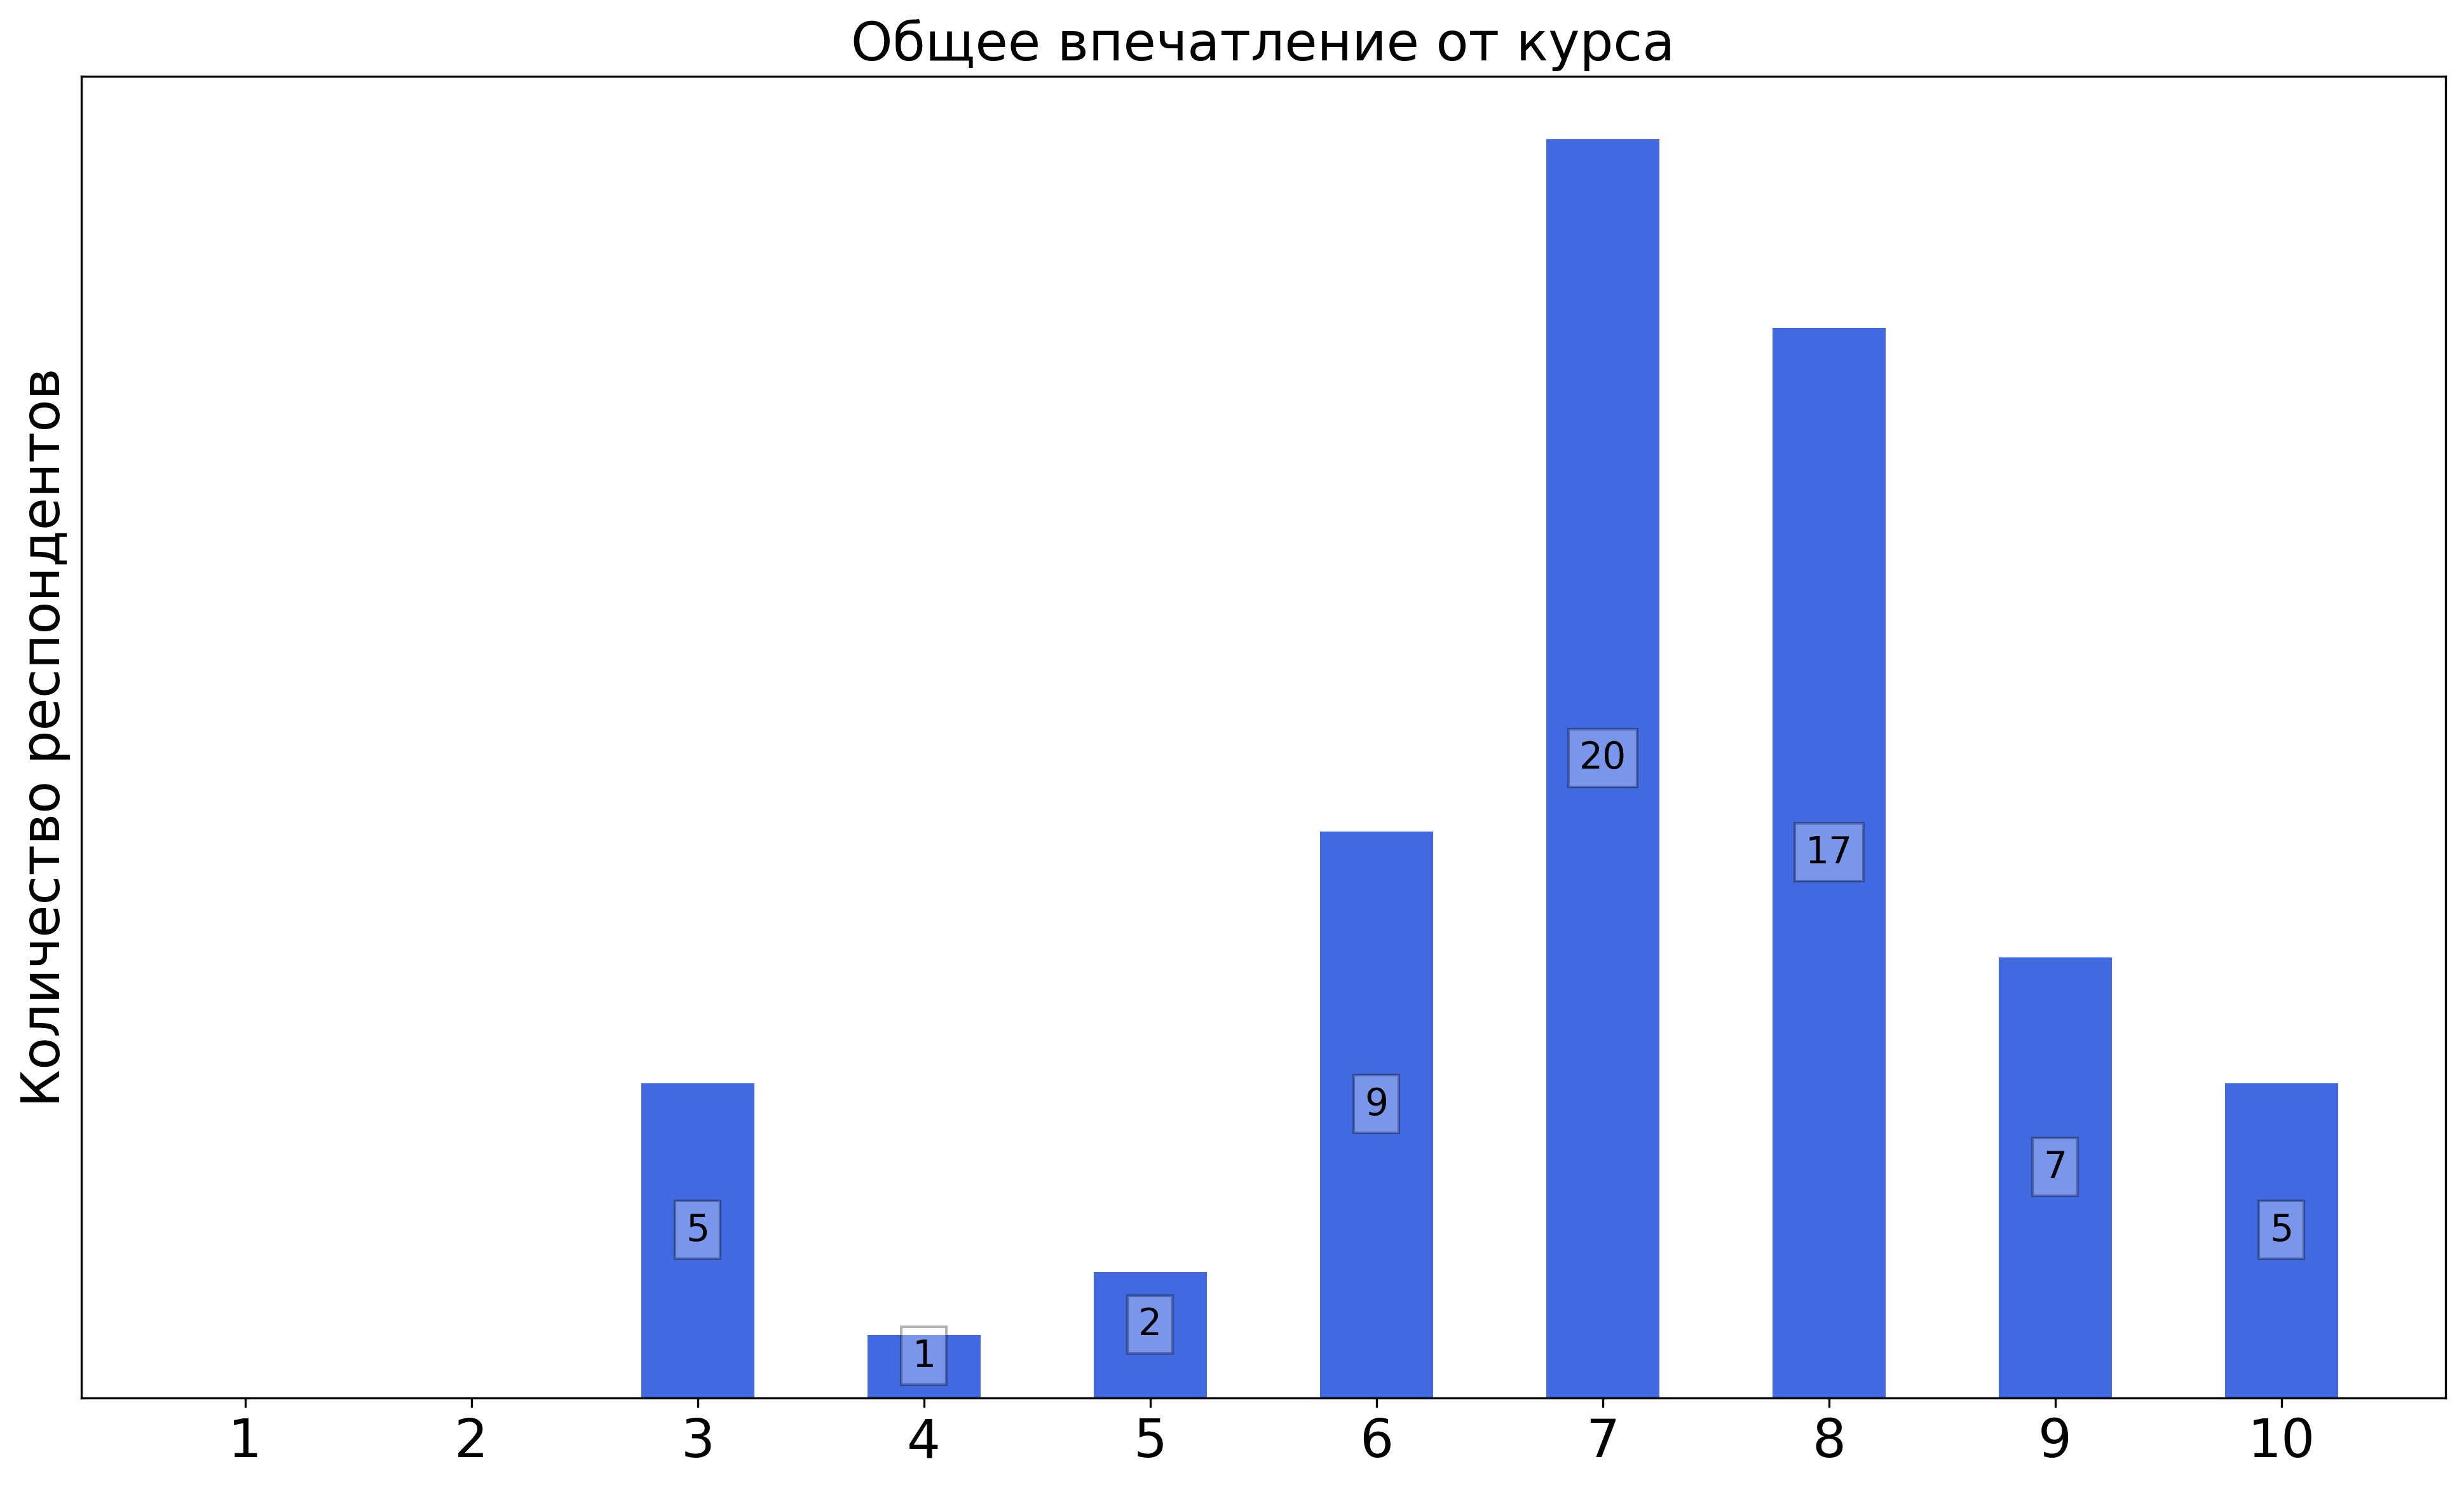
\includegraphics[width=\textwidth]{images/1 course/Общая физика - механика/general-0.png}
			\end{subfigure}
			\begin{subfigure}[b]{0.45\textwidth}
				\centering
				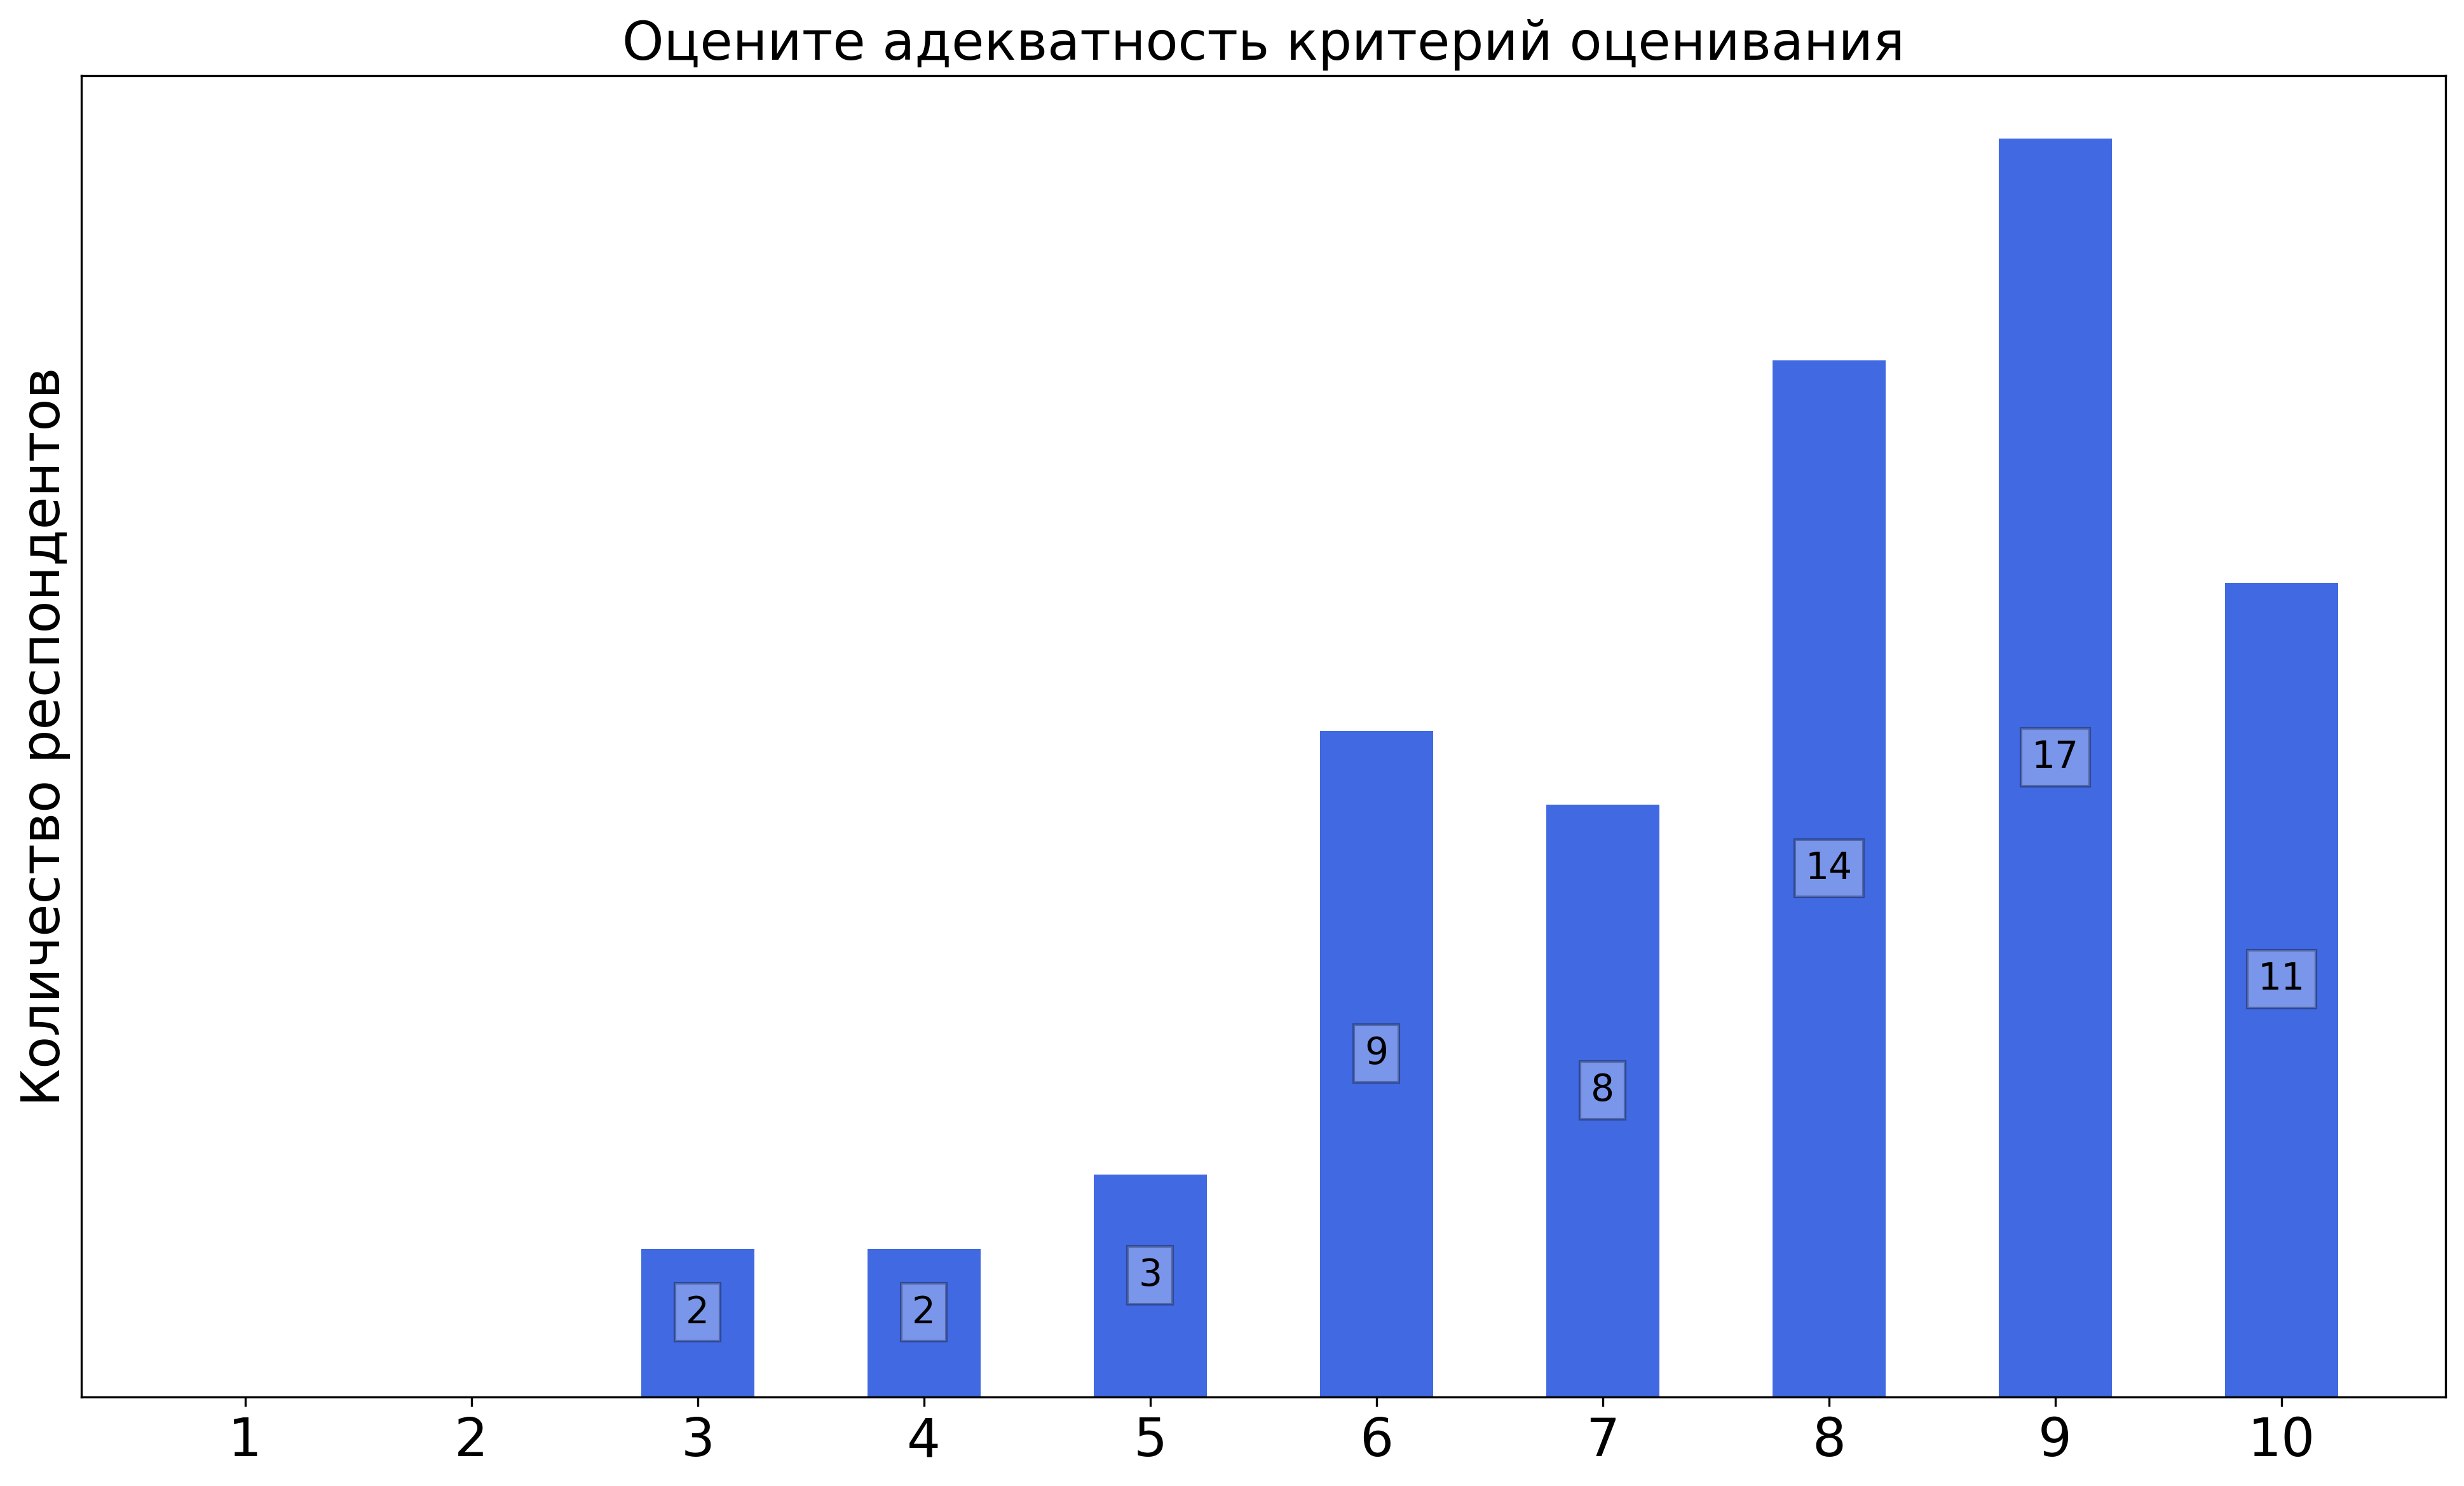
\includegraphics[width=\textwidth]{images/1 course/Общая физика - механика/general-1.png}
			\end{subfigure}	
		\end{figure}

	\subsubsection{Материалы, использумые респондентами при изучении курса}

		\begin{figure}[H]
			\centering
			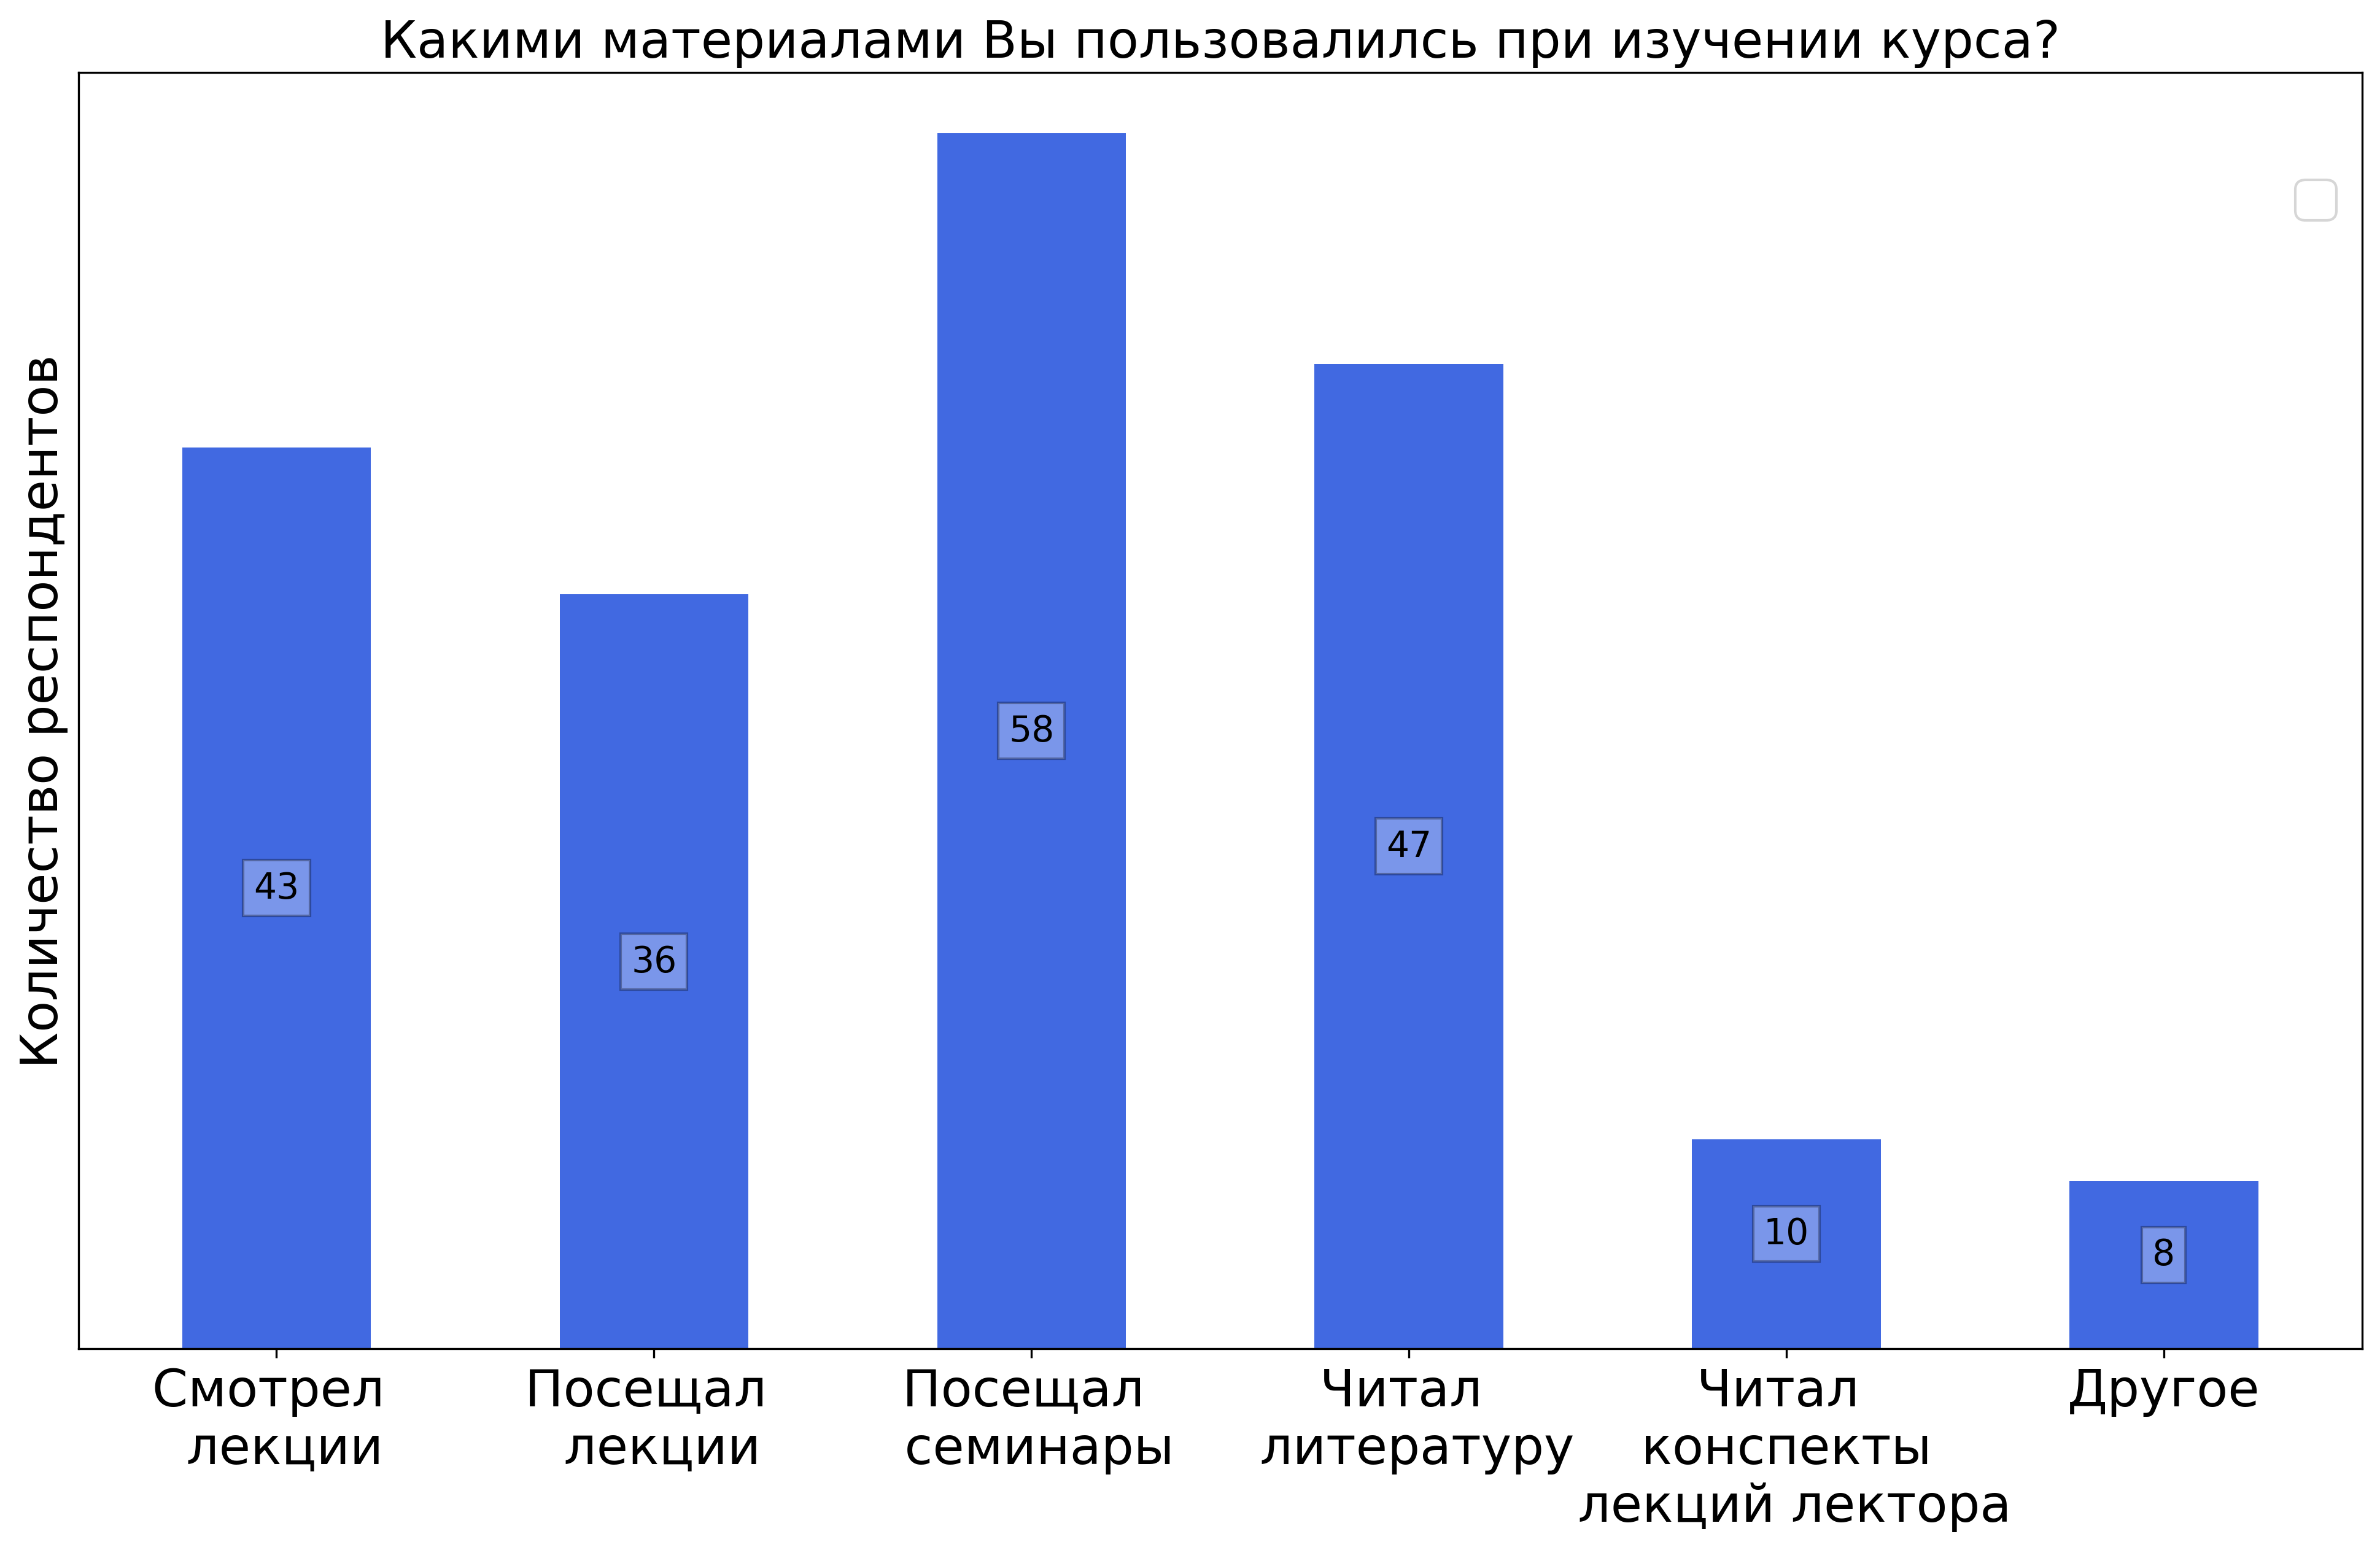
\includegraphics[width = 0.45\textwidth]{images/1 course/Общая физика - механика/materials.png}
		\end{figure}

		\textit{В качестве других источников информации студенты указали:} 
		\begin{itemize}
			\item онлайн-консультации по билетам к экзамену;
			\item семинары других преподавателей;
			\item материалы из интернета;
			\item доп. семинары Овчинкина В.А.
		\end{itemize}

	\subsubsection{Отзыв студентов о лекциях. Лектор: Холин Д.И.}

		\begin{figure}[H]
			\centering
            \begin{subfigure}[b]{0.45\textwidth}
				\centering
				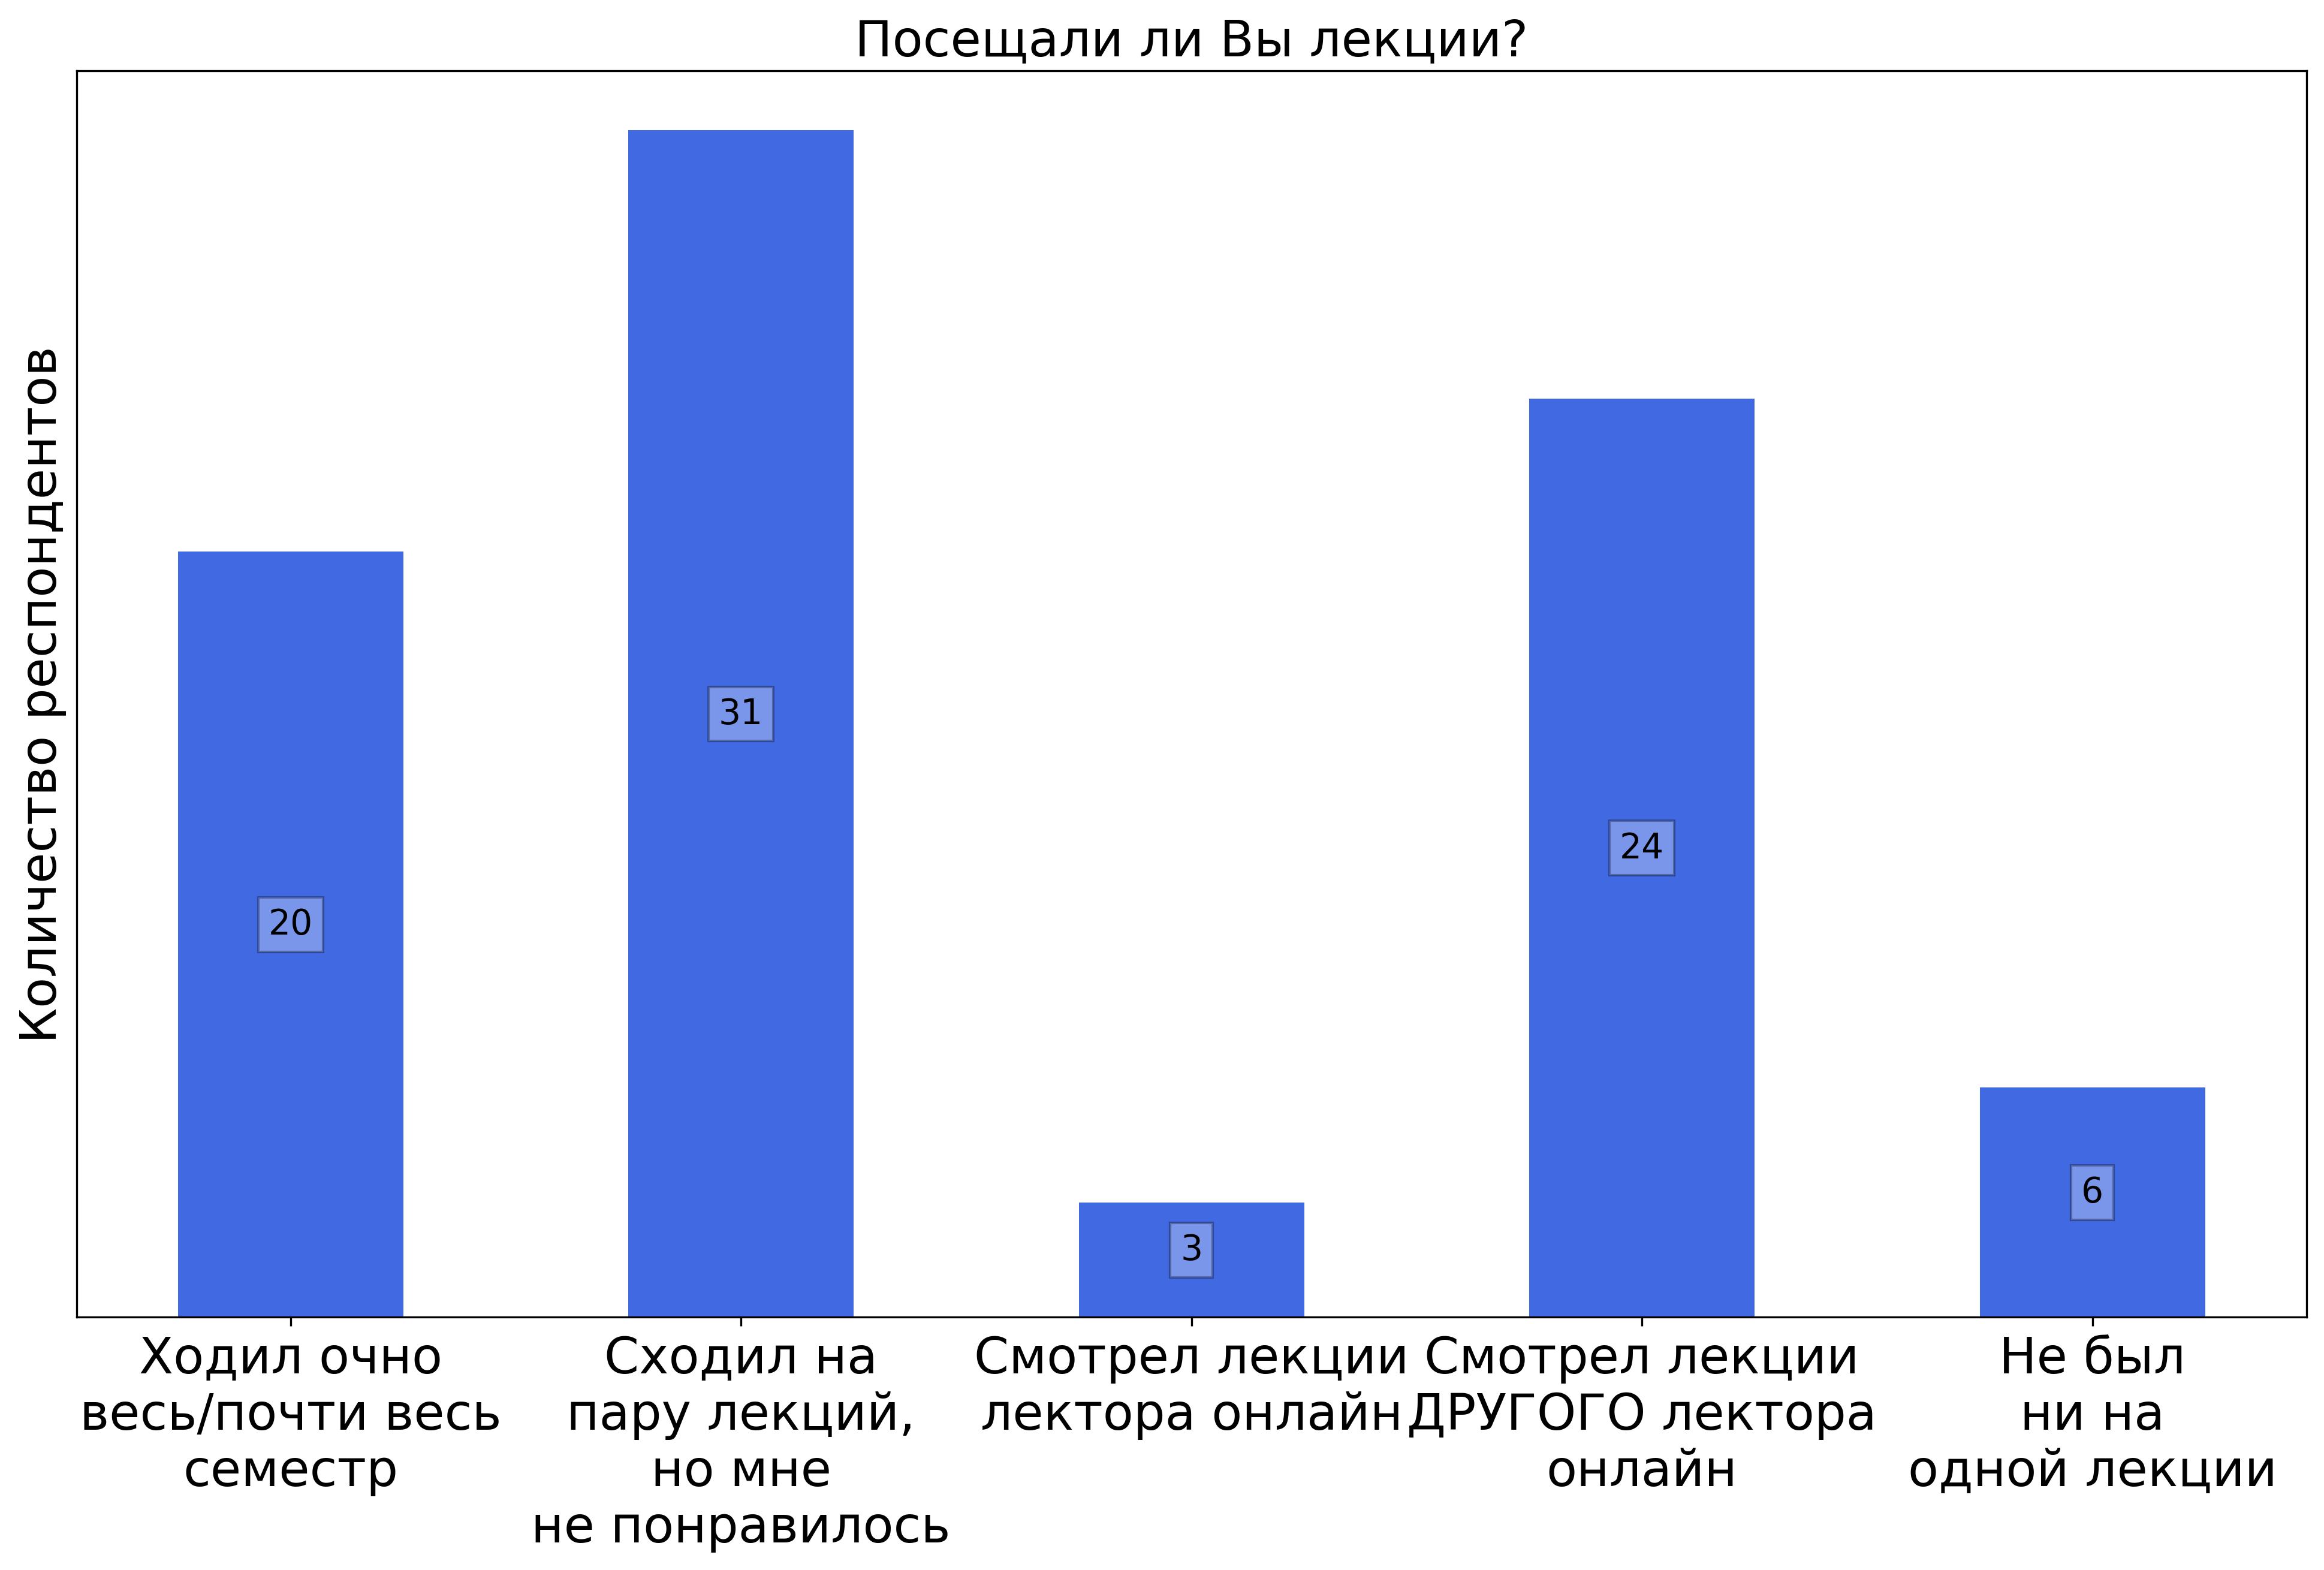
\includegraphics[width=\textwidth]{images/1 course/Общая физика - механика/lecturer-questions-Холин Д.И.-0.png}
			\end{subfigure}
			\begin{subfigure}[b]{0.45\textwidth}
				\centering
				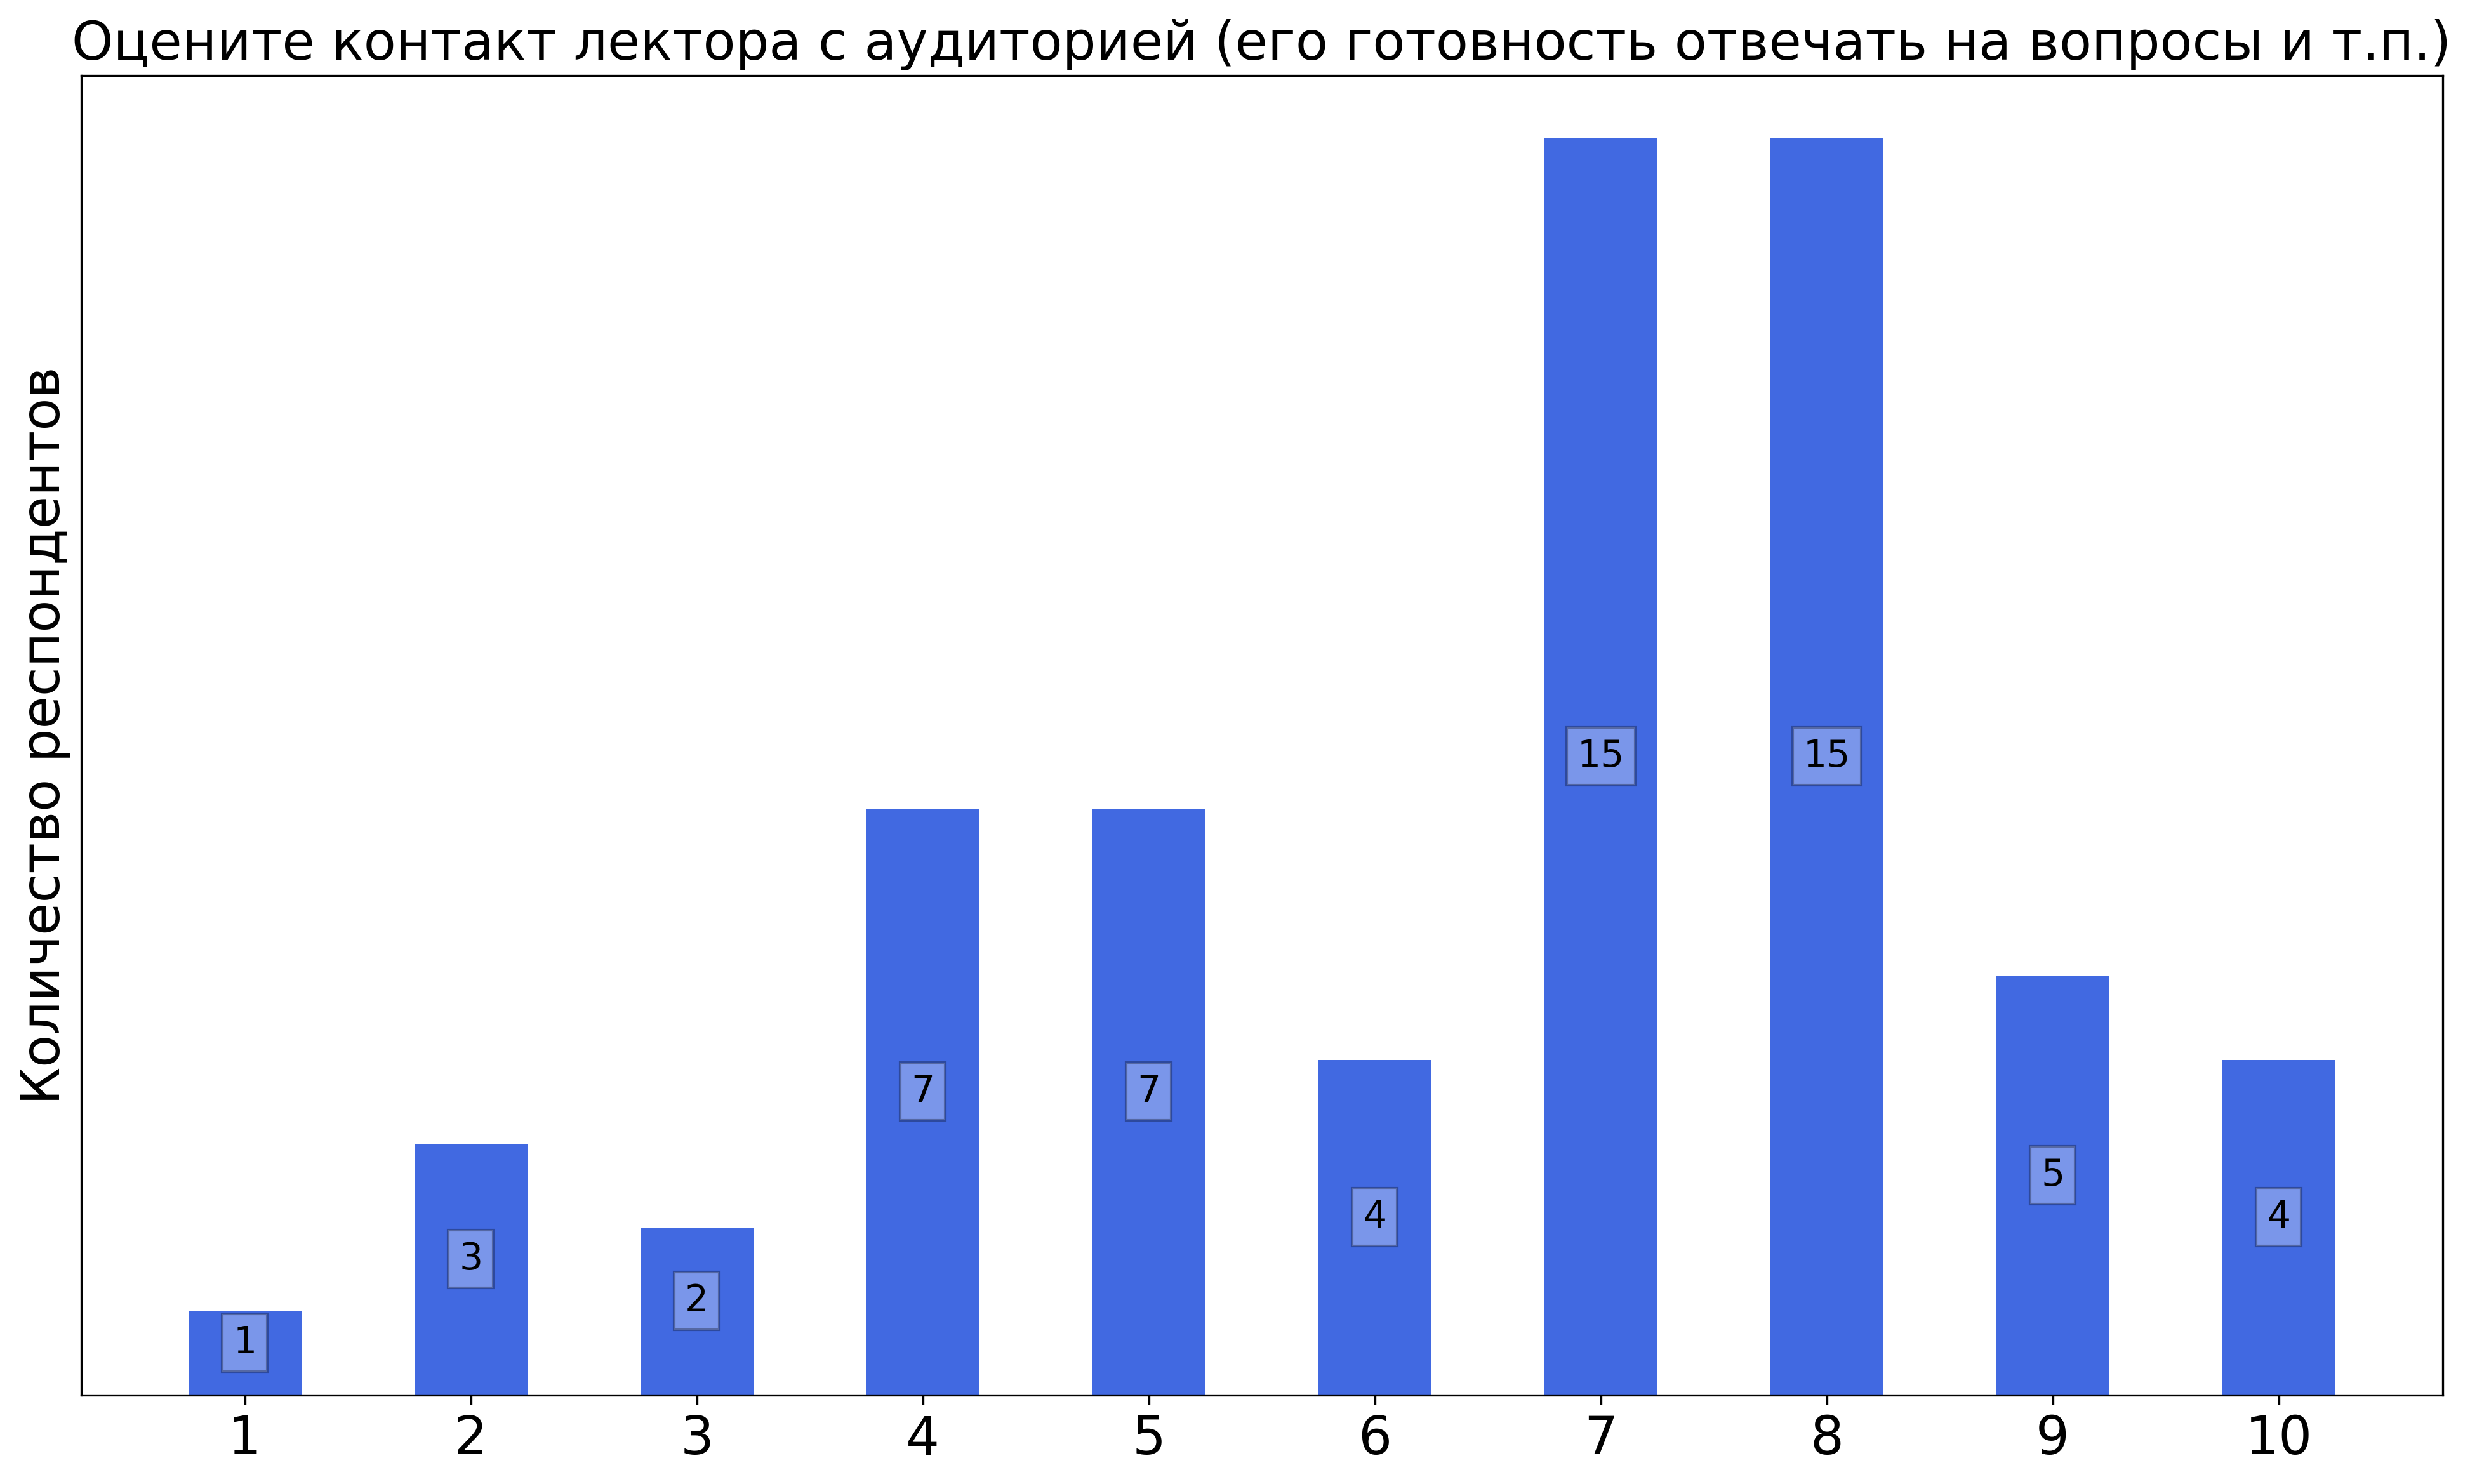
\includegraphics[width=\textwidth]{images/1 course/Общая физика - механика/lecturer-marks-Холин Д.И.-0.png}
			\end{subfigure}
			\begin{subfigure}[b]{0.45\textwidth}
				\centering
				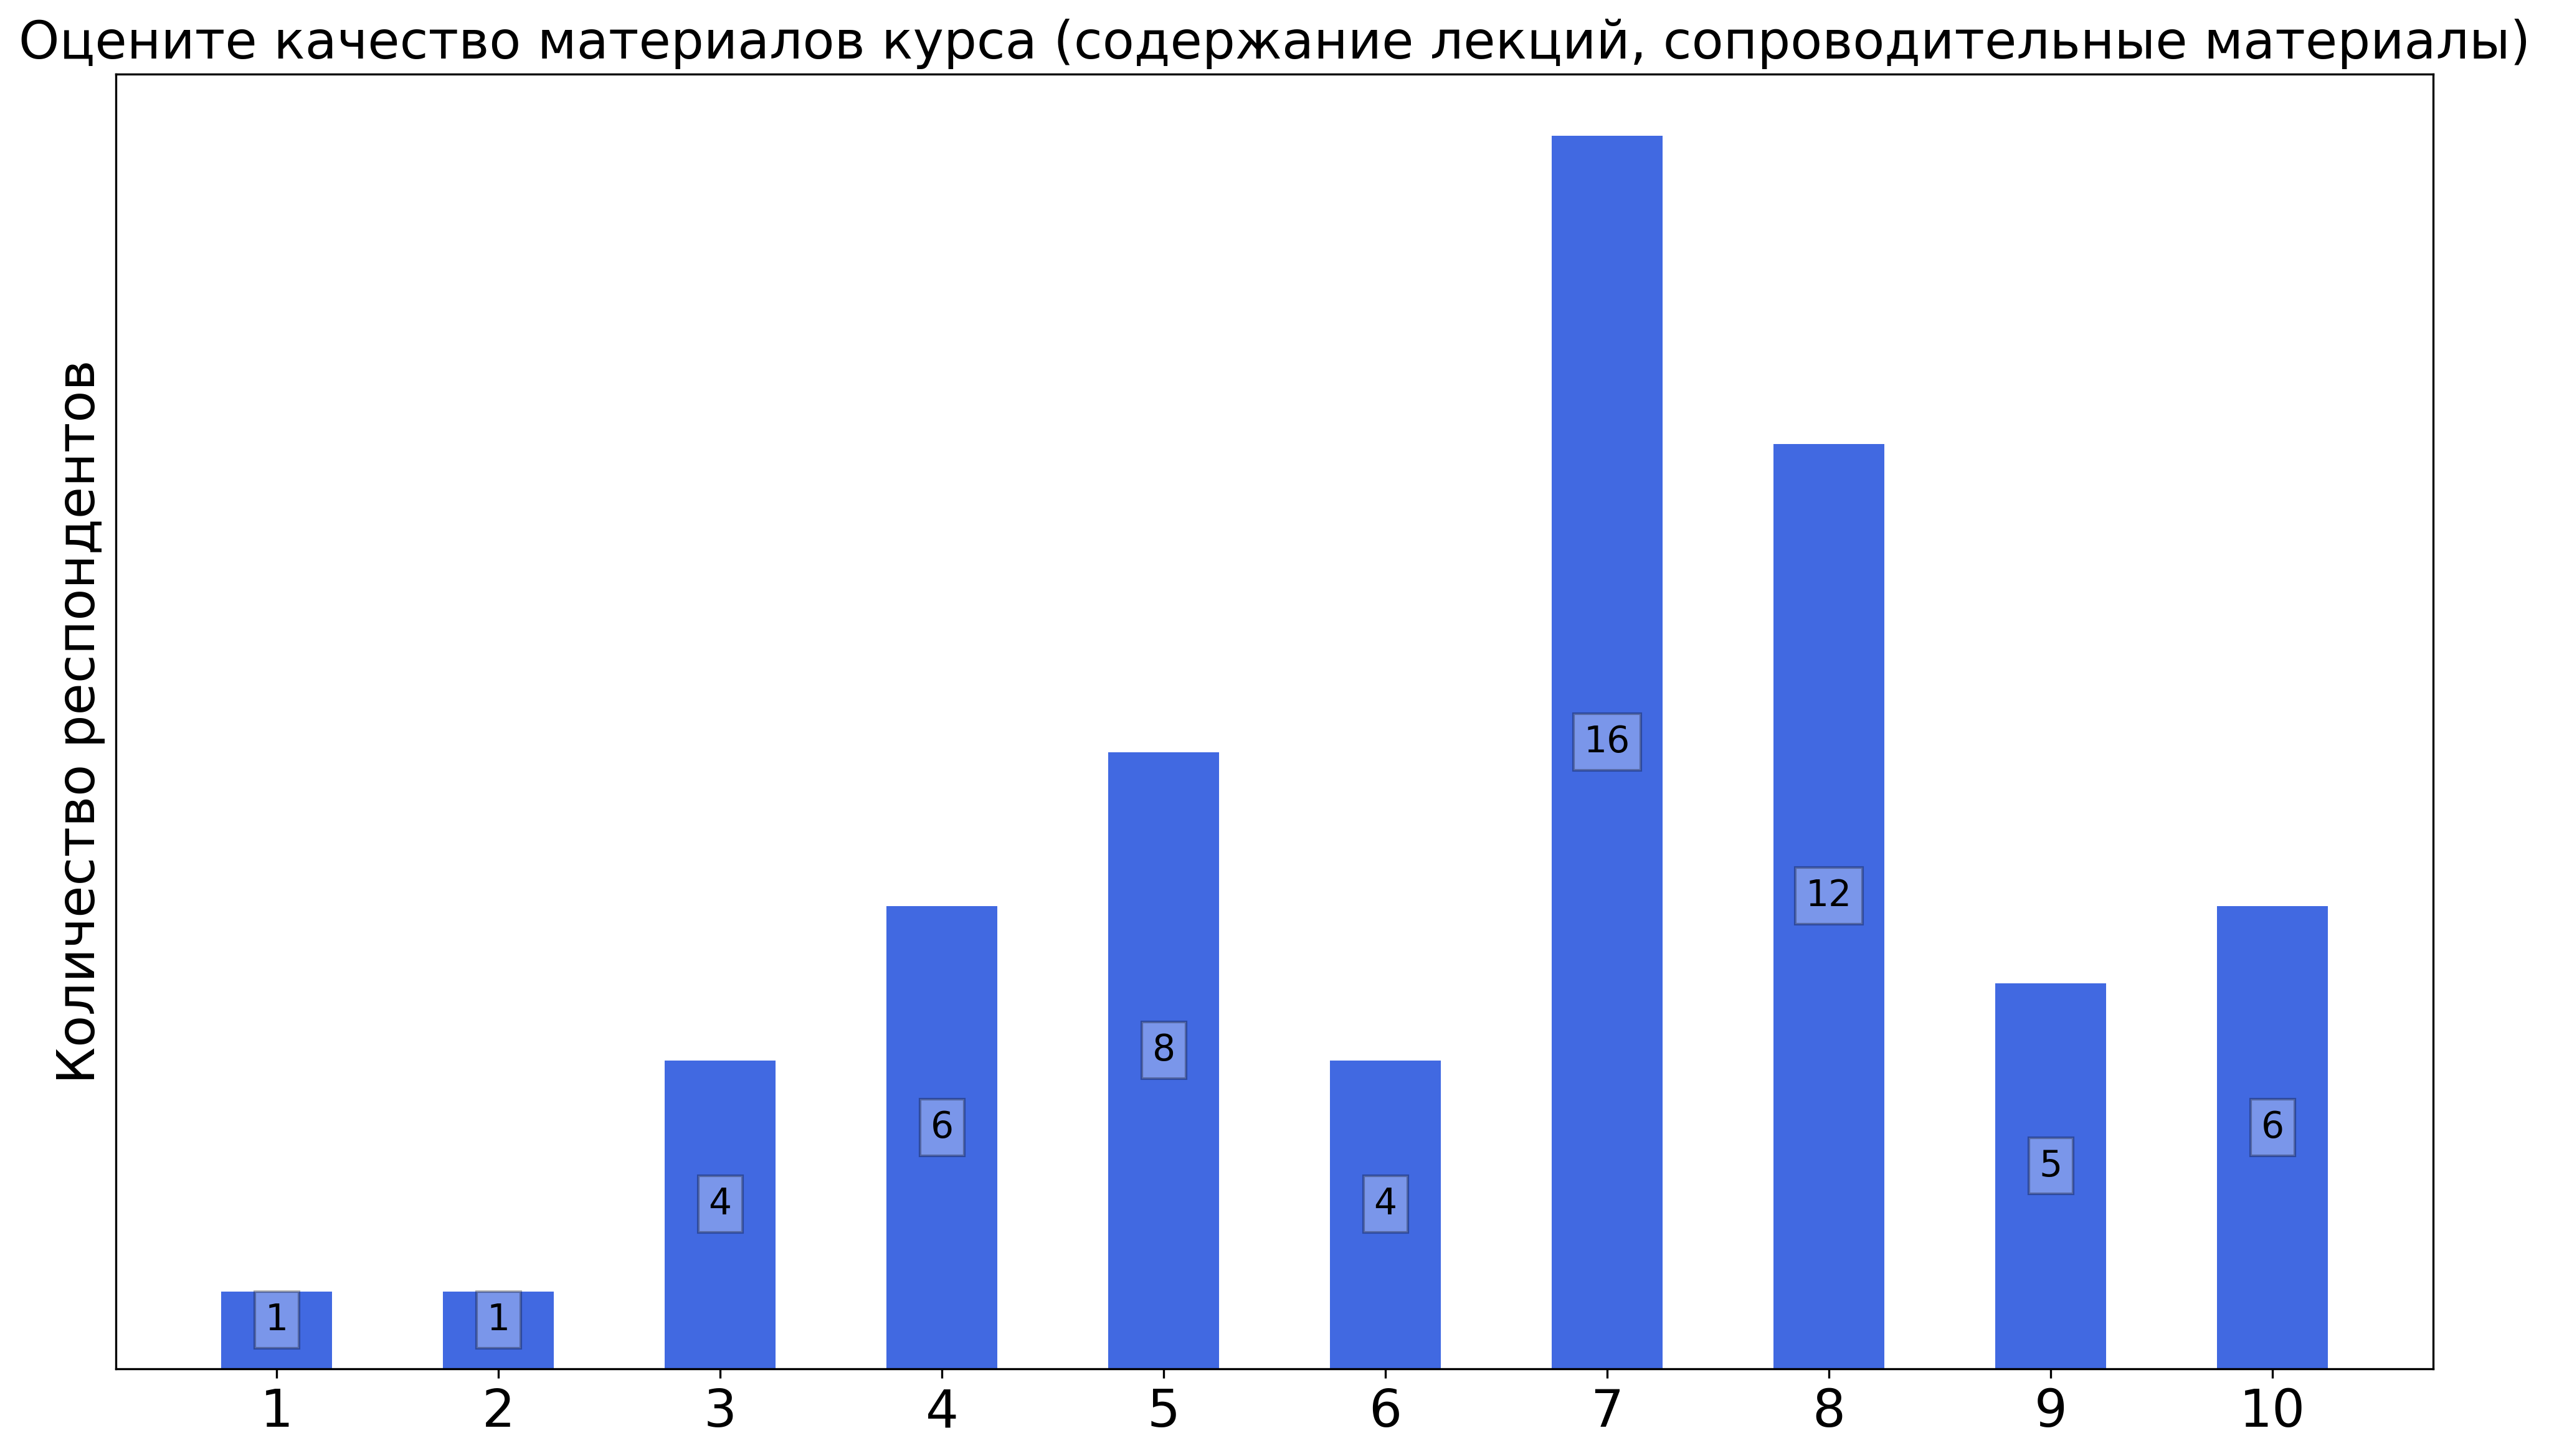
\includegraphics[width=\textwidth]{images/1 course/Общая физика - механика/lecturer-marks-Холин Д.И.-1.png}
			\end{subfigure}
			\begin{subfigure}[b]{0.45\textwidth}
				\centering
				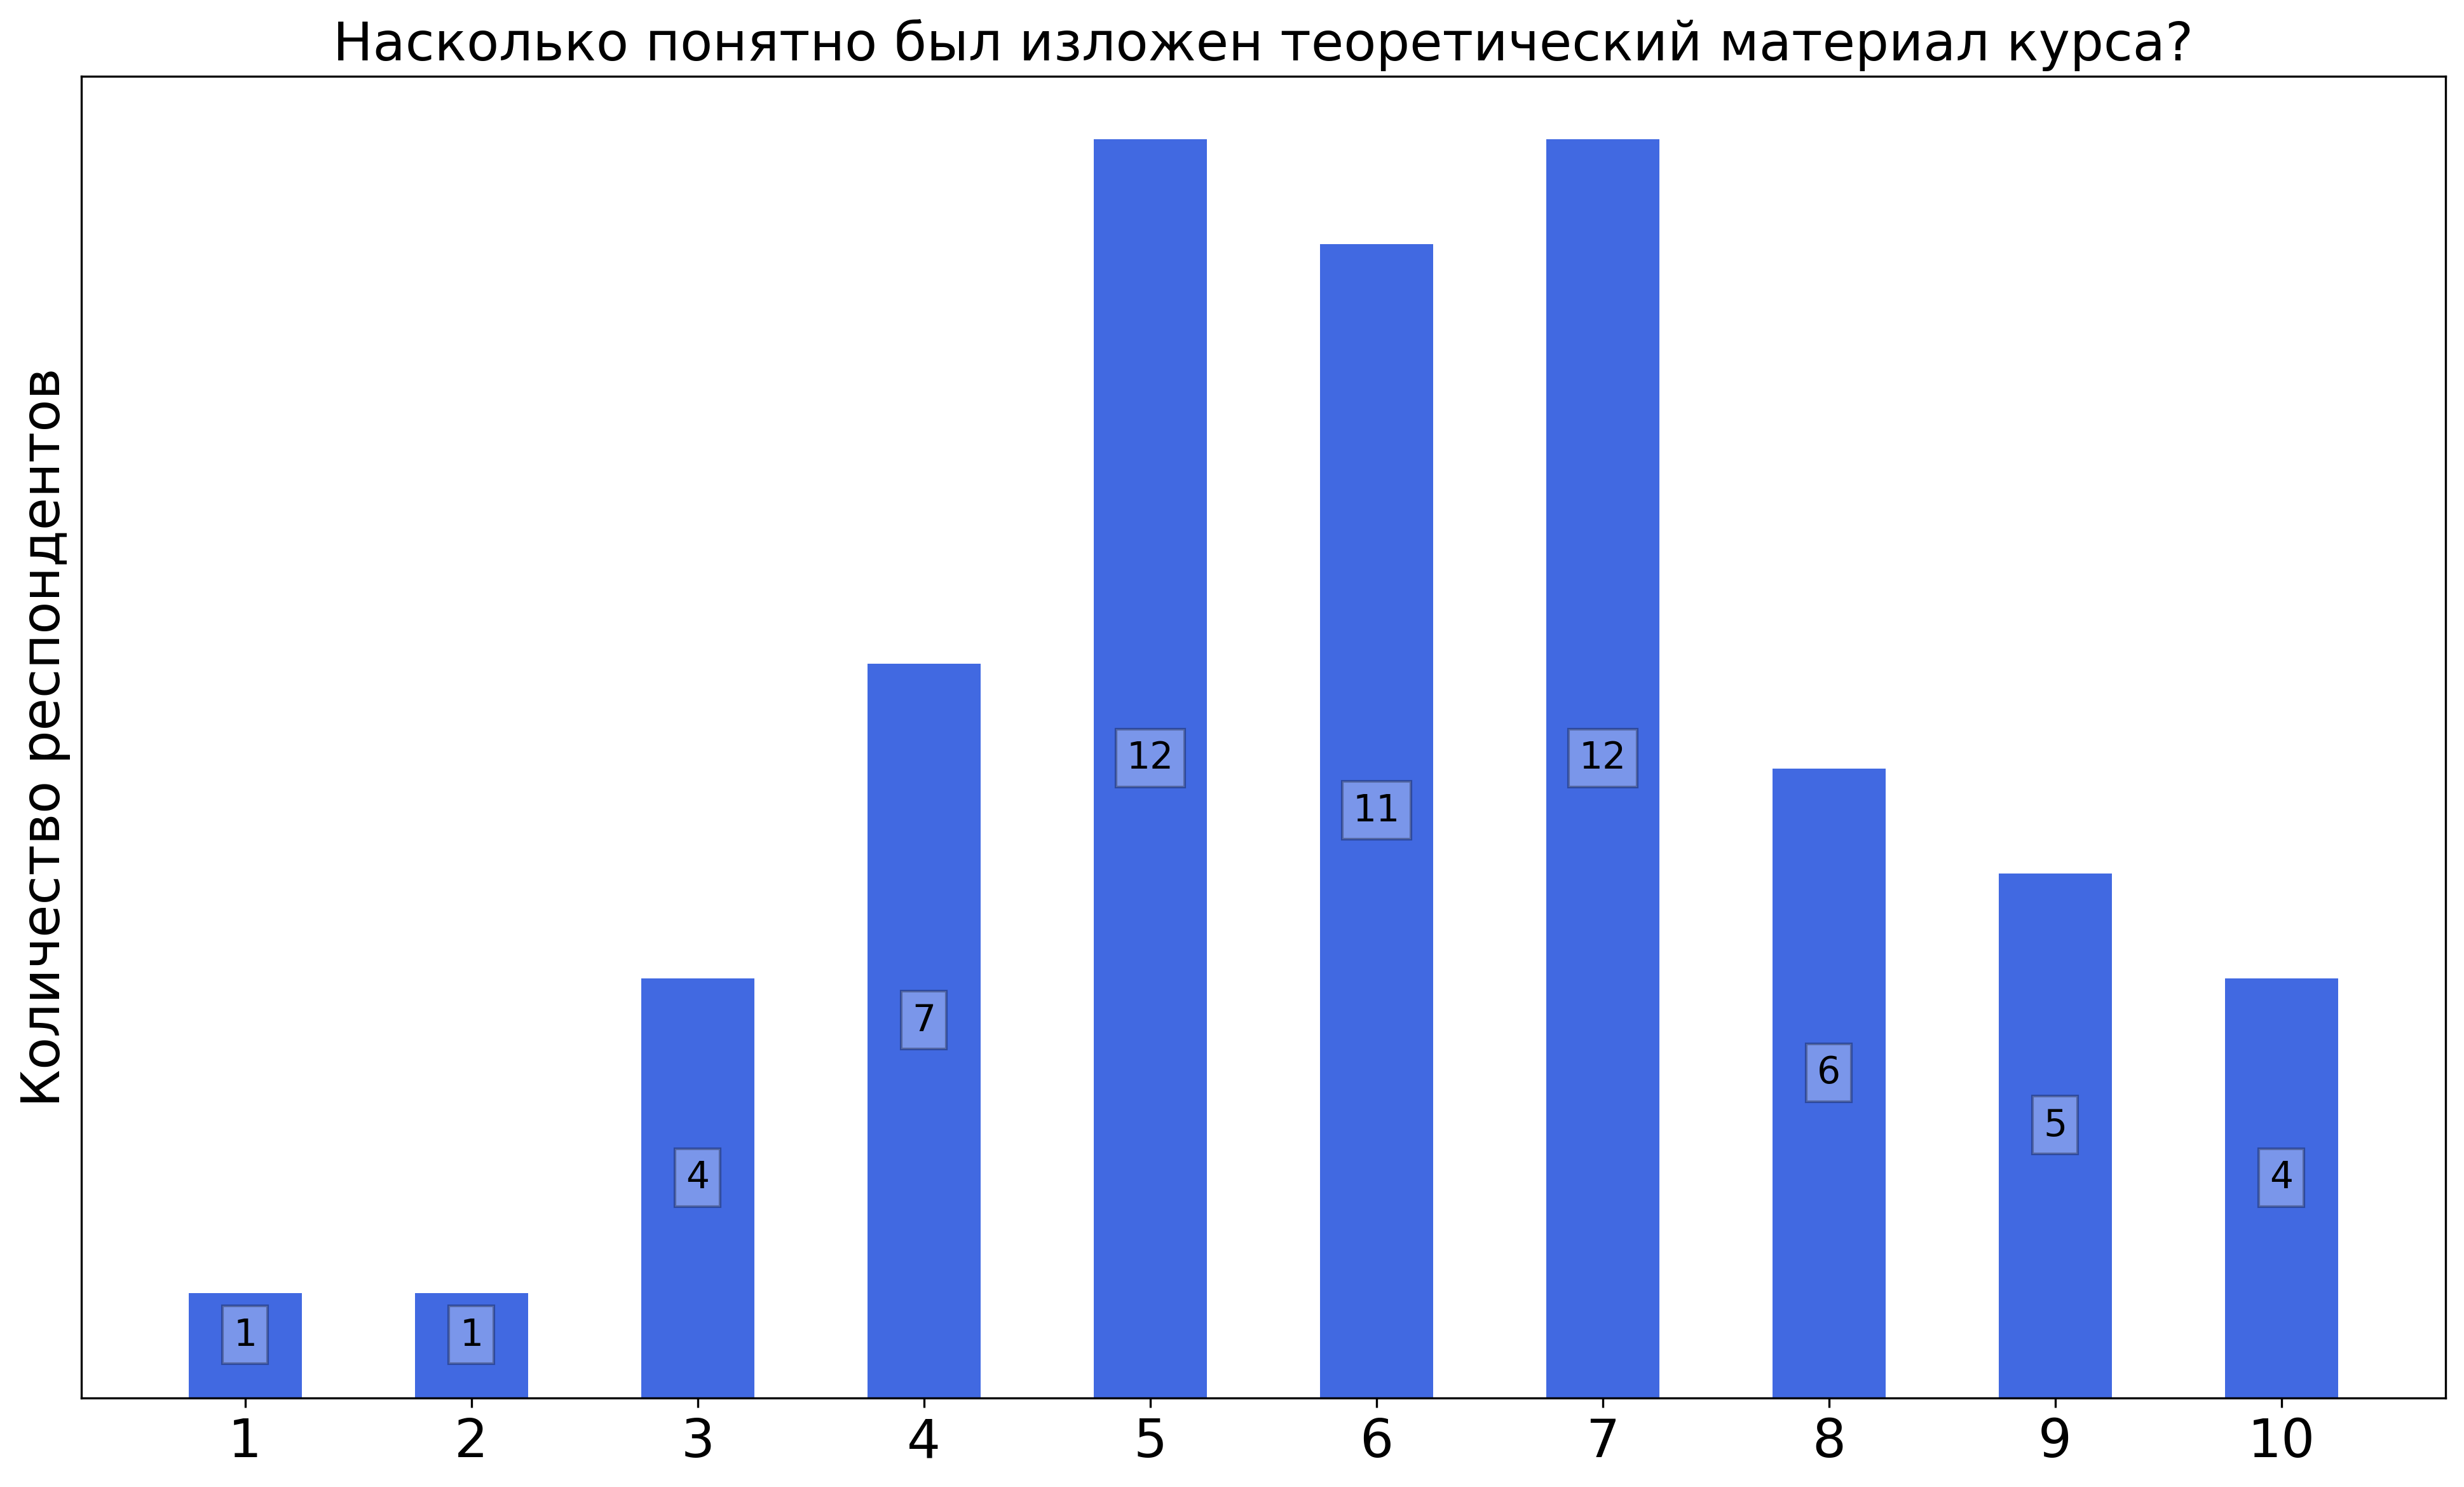
\includegraphics[width=\textwidth]{images/1 course/Общая физика - механика/lecturer-marks-Холин Д.И.-2.png}
			\end{subfigure}	
			\begin{subfigure}[b]{0.45\textwidth}
				\centering
				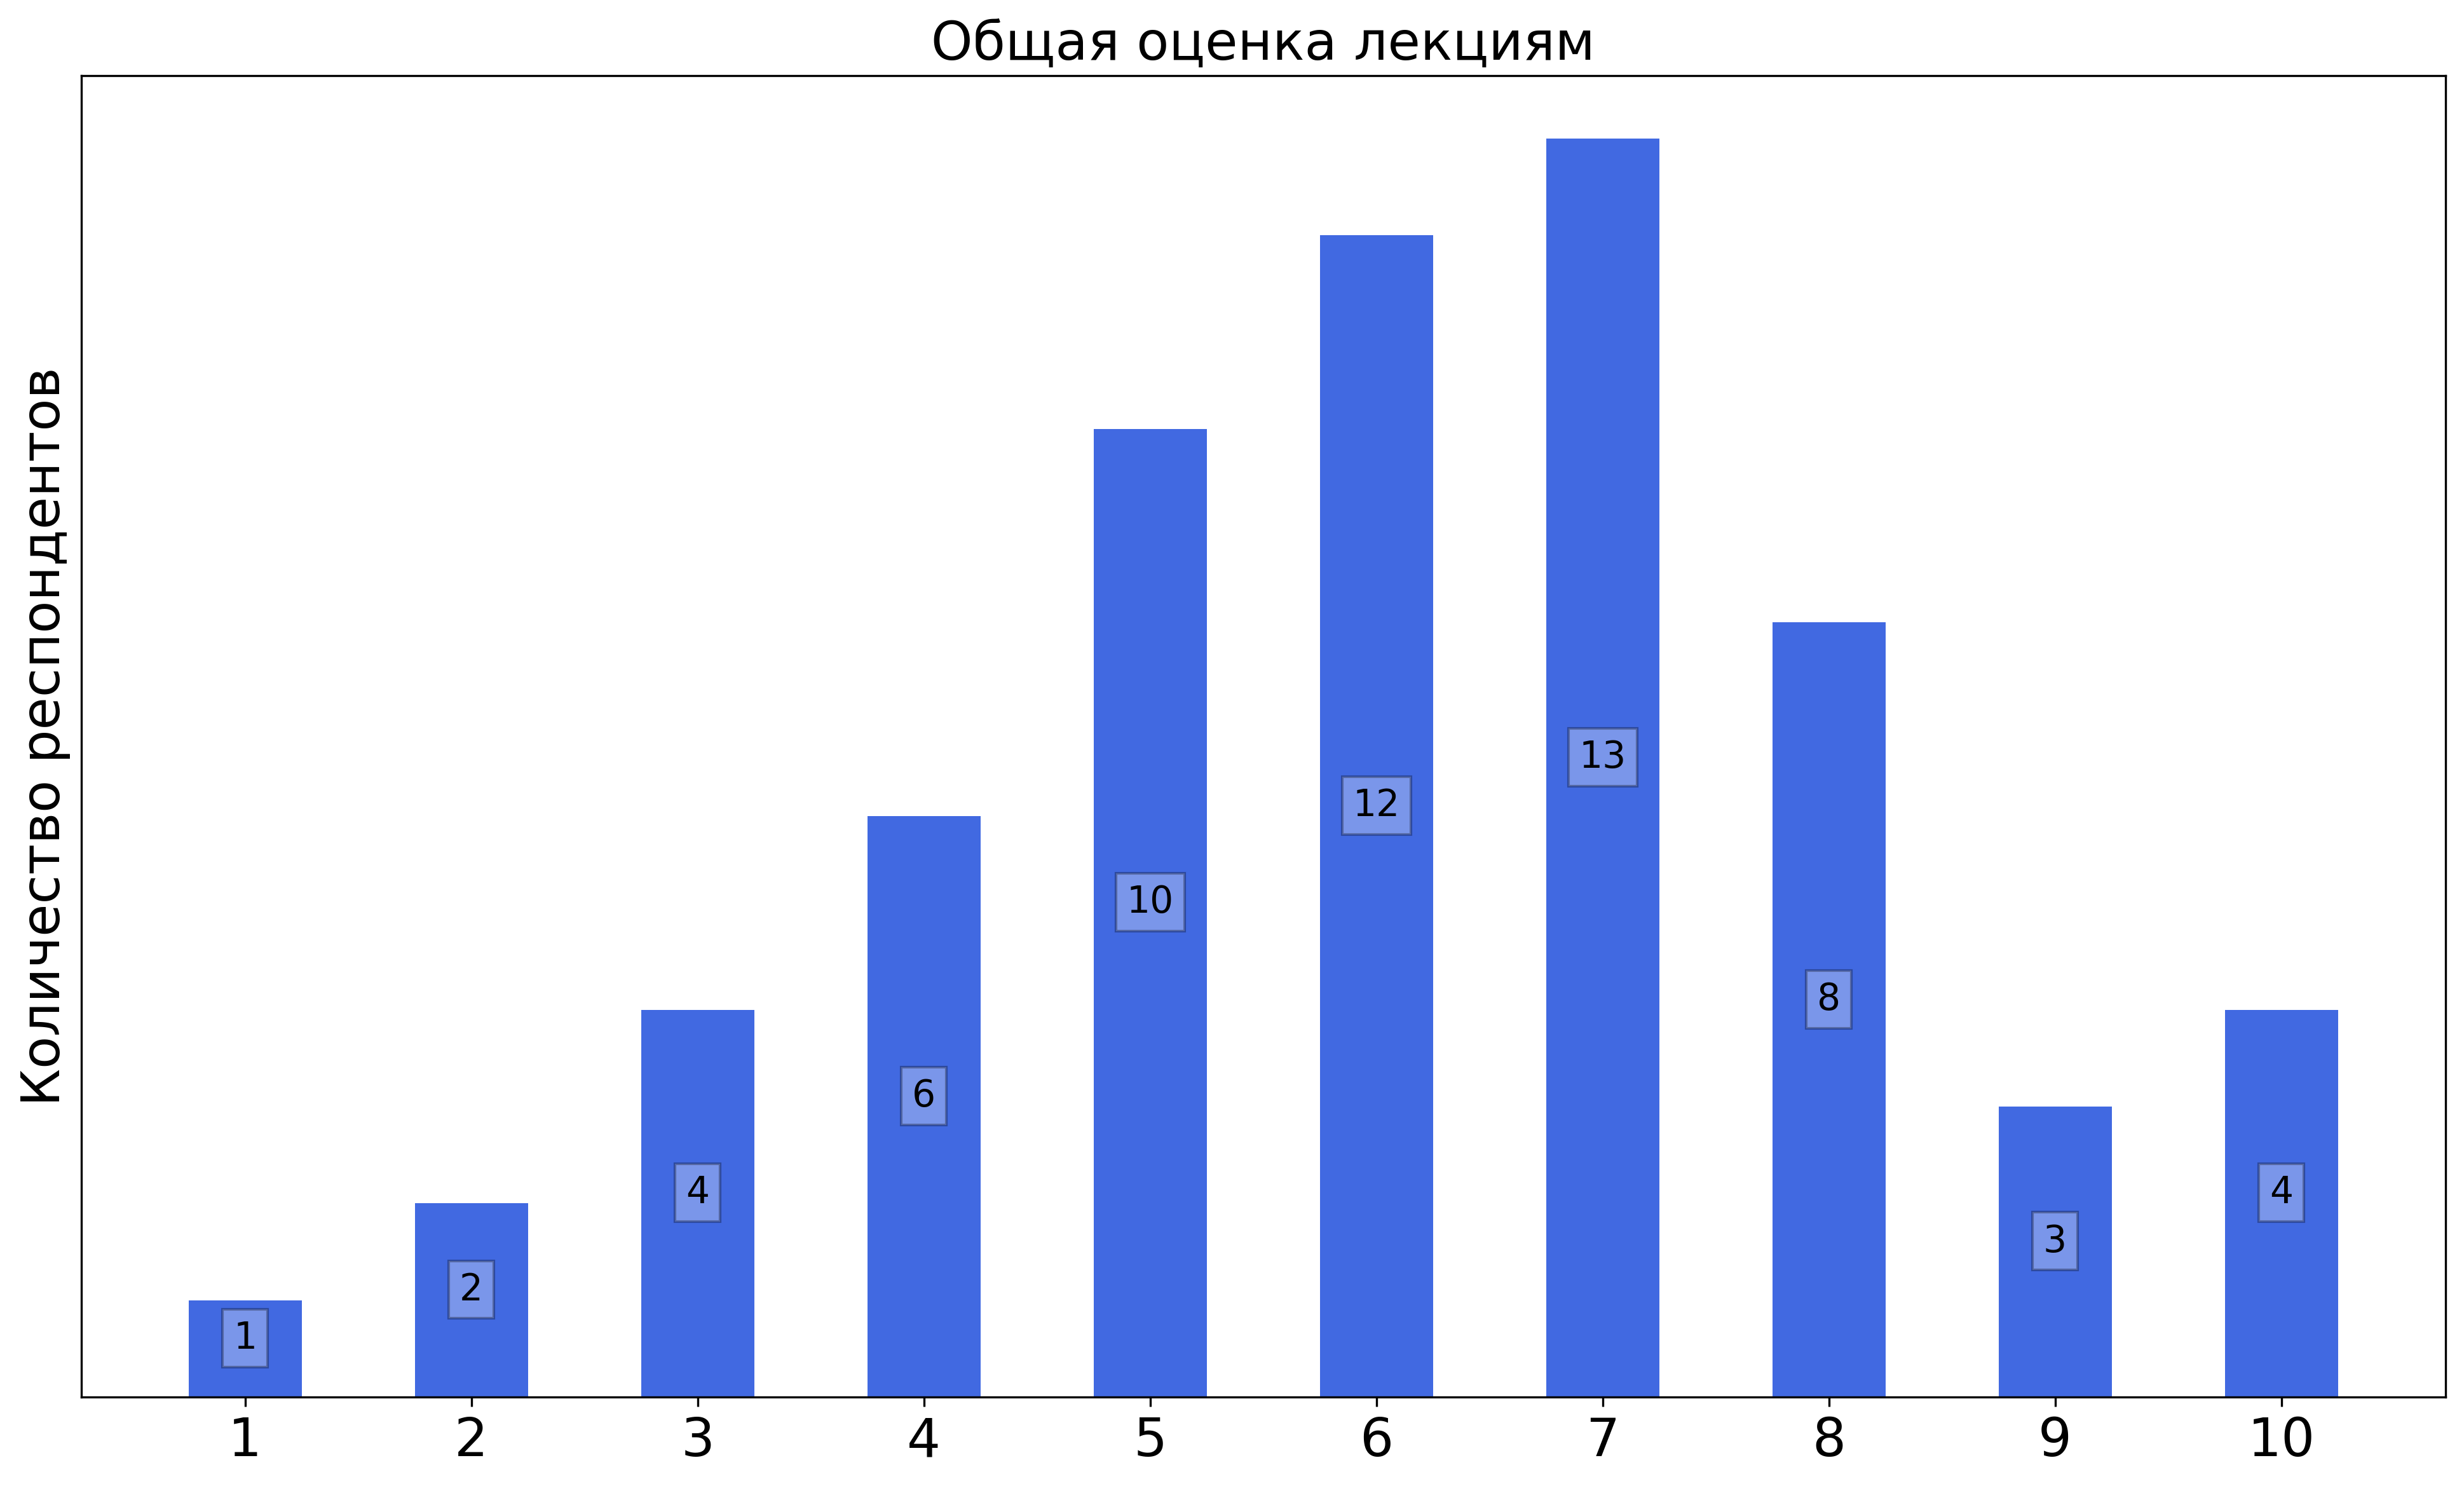
\includegraphics[width=\textwidth]{images/1 course/Общая физика - механика/lecturer-marks-Холин Д.И.-3.png}
			\end{subfigure}
			\caption{Оценки респондентов о качестве преподавания лекций по курсу <<Общая физика: механика>>}
		\end{figure}

		\textbf{Комментарии студентов о лекциях\protect\footnote{сохранены оригинальные орфография и пунктуация}}

            \begin{commentbox} 
                На лекциях складыаается ощущение, что преподаватель сам не разбирается в материале, потому что он рассказывает материал только со своими листочками, в которые постоянно смотрит, забывая то, что хотел сказать. Объясняет достаточно тихо и нудно, все, кто ходил к нему на лекции, засыпали. Рассказал далеко не все, некоторые темы из экзаменационной програмиы пропустил, оставив на самостоятельное изучение. На вопросы отвечает, хотя понимание материала несильно увеличивается. 
            \end{commentbox} 
        
            \begin{commentbox} 
                Лектор хороший, иногда рассказывает о связанных с темой вещах. Особо не акцентирует внимание на полном доказательстве теории и определениях, что немного осложняет поиск информации для экзамена, но затрагивает все темы курса 
            \end{commentbox} 
        
            \begin{commentbox} 
                Читает с своих конспектов, самостоятельно может не сразу сформулировать нужное высказывание или доказательство 
            \end{commentbox} 
        
            \begin{commentbox} 
                Мне больше понравилось смотреть лекции Колдунова 
            \end{commentbox} 
        
            \begin{commentbox} 
                Всё устраивает 
            \end{commentbox} 
        
            \begin{commentbox} 
                Здесь выставлены оценки для лектора, которого смотрел я(Булыгин). Холину ставлю 5. 
            \end{commentbox} 
        
            \begin{commentbox} 
                без своих заранее написанных бумажек не может выстроить лекцию, постоянно путается в своих же записях, вследствие чего тормозится лекция 
            \end{commentbox} 
        
            \begin{commentbox} 
                ничего не понятно 
            \end{commentbox} 
        
            \begin{commentbox} 
                Я не смог слушать, так как его голос меня усыплял. На паре до лекции по физике я сидел нормально и был вовлечен, а приходил на физику и даже глаза не мог открыть.  
            \end{commentbox} 
        
            \begin{commentbox} 
                Холин плох, объективно, поэтому все смотрят овчоса или попова 
            \end{commentbox} 
        
            \begin{commentbox} 
                Неплохо, но есть варианты получше 
            \end{commentbox} 
        
            \begin{commentbox} 
                Большая часть материала преподносится нестрого и непонятно. По материалам этих лекций нельзя готовиться к сдаче экзамена 
            \end{commentbox} 
        
            \begin{commentbox} 
                В целом нормальные лекции, но Холин не успевает рассказать всё, что нужно, иногда забывает, как что-то доказывается и тупит пару минут, смотря в доску.  
            \end{commentbox} 
        
            \begin{commentbox} 
                Не всякая лекция Холина Д.И. по механике была интересной и доступно изложенной... 
            \end{commentbox} 

	\subsubsection{Отзыв студентов о семинарах. Семинарист: Вановский В.В.}
		\begin{figure}[H]
			\centering
			\begin{subfigure}[b]{0.45\textwidth}
				\centering
				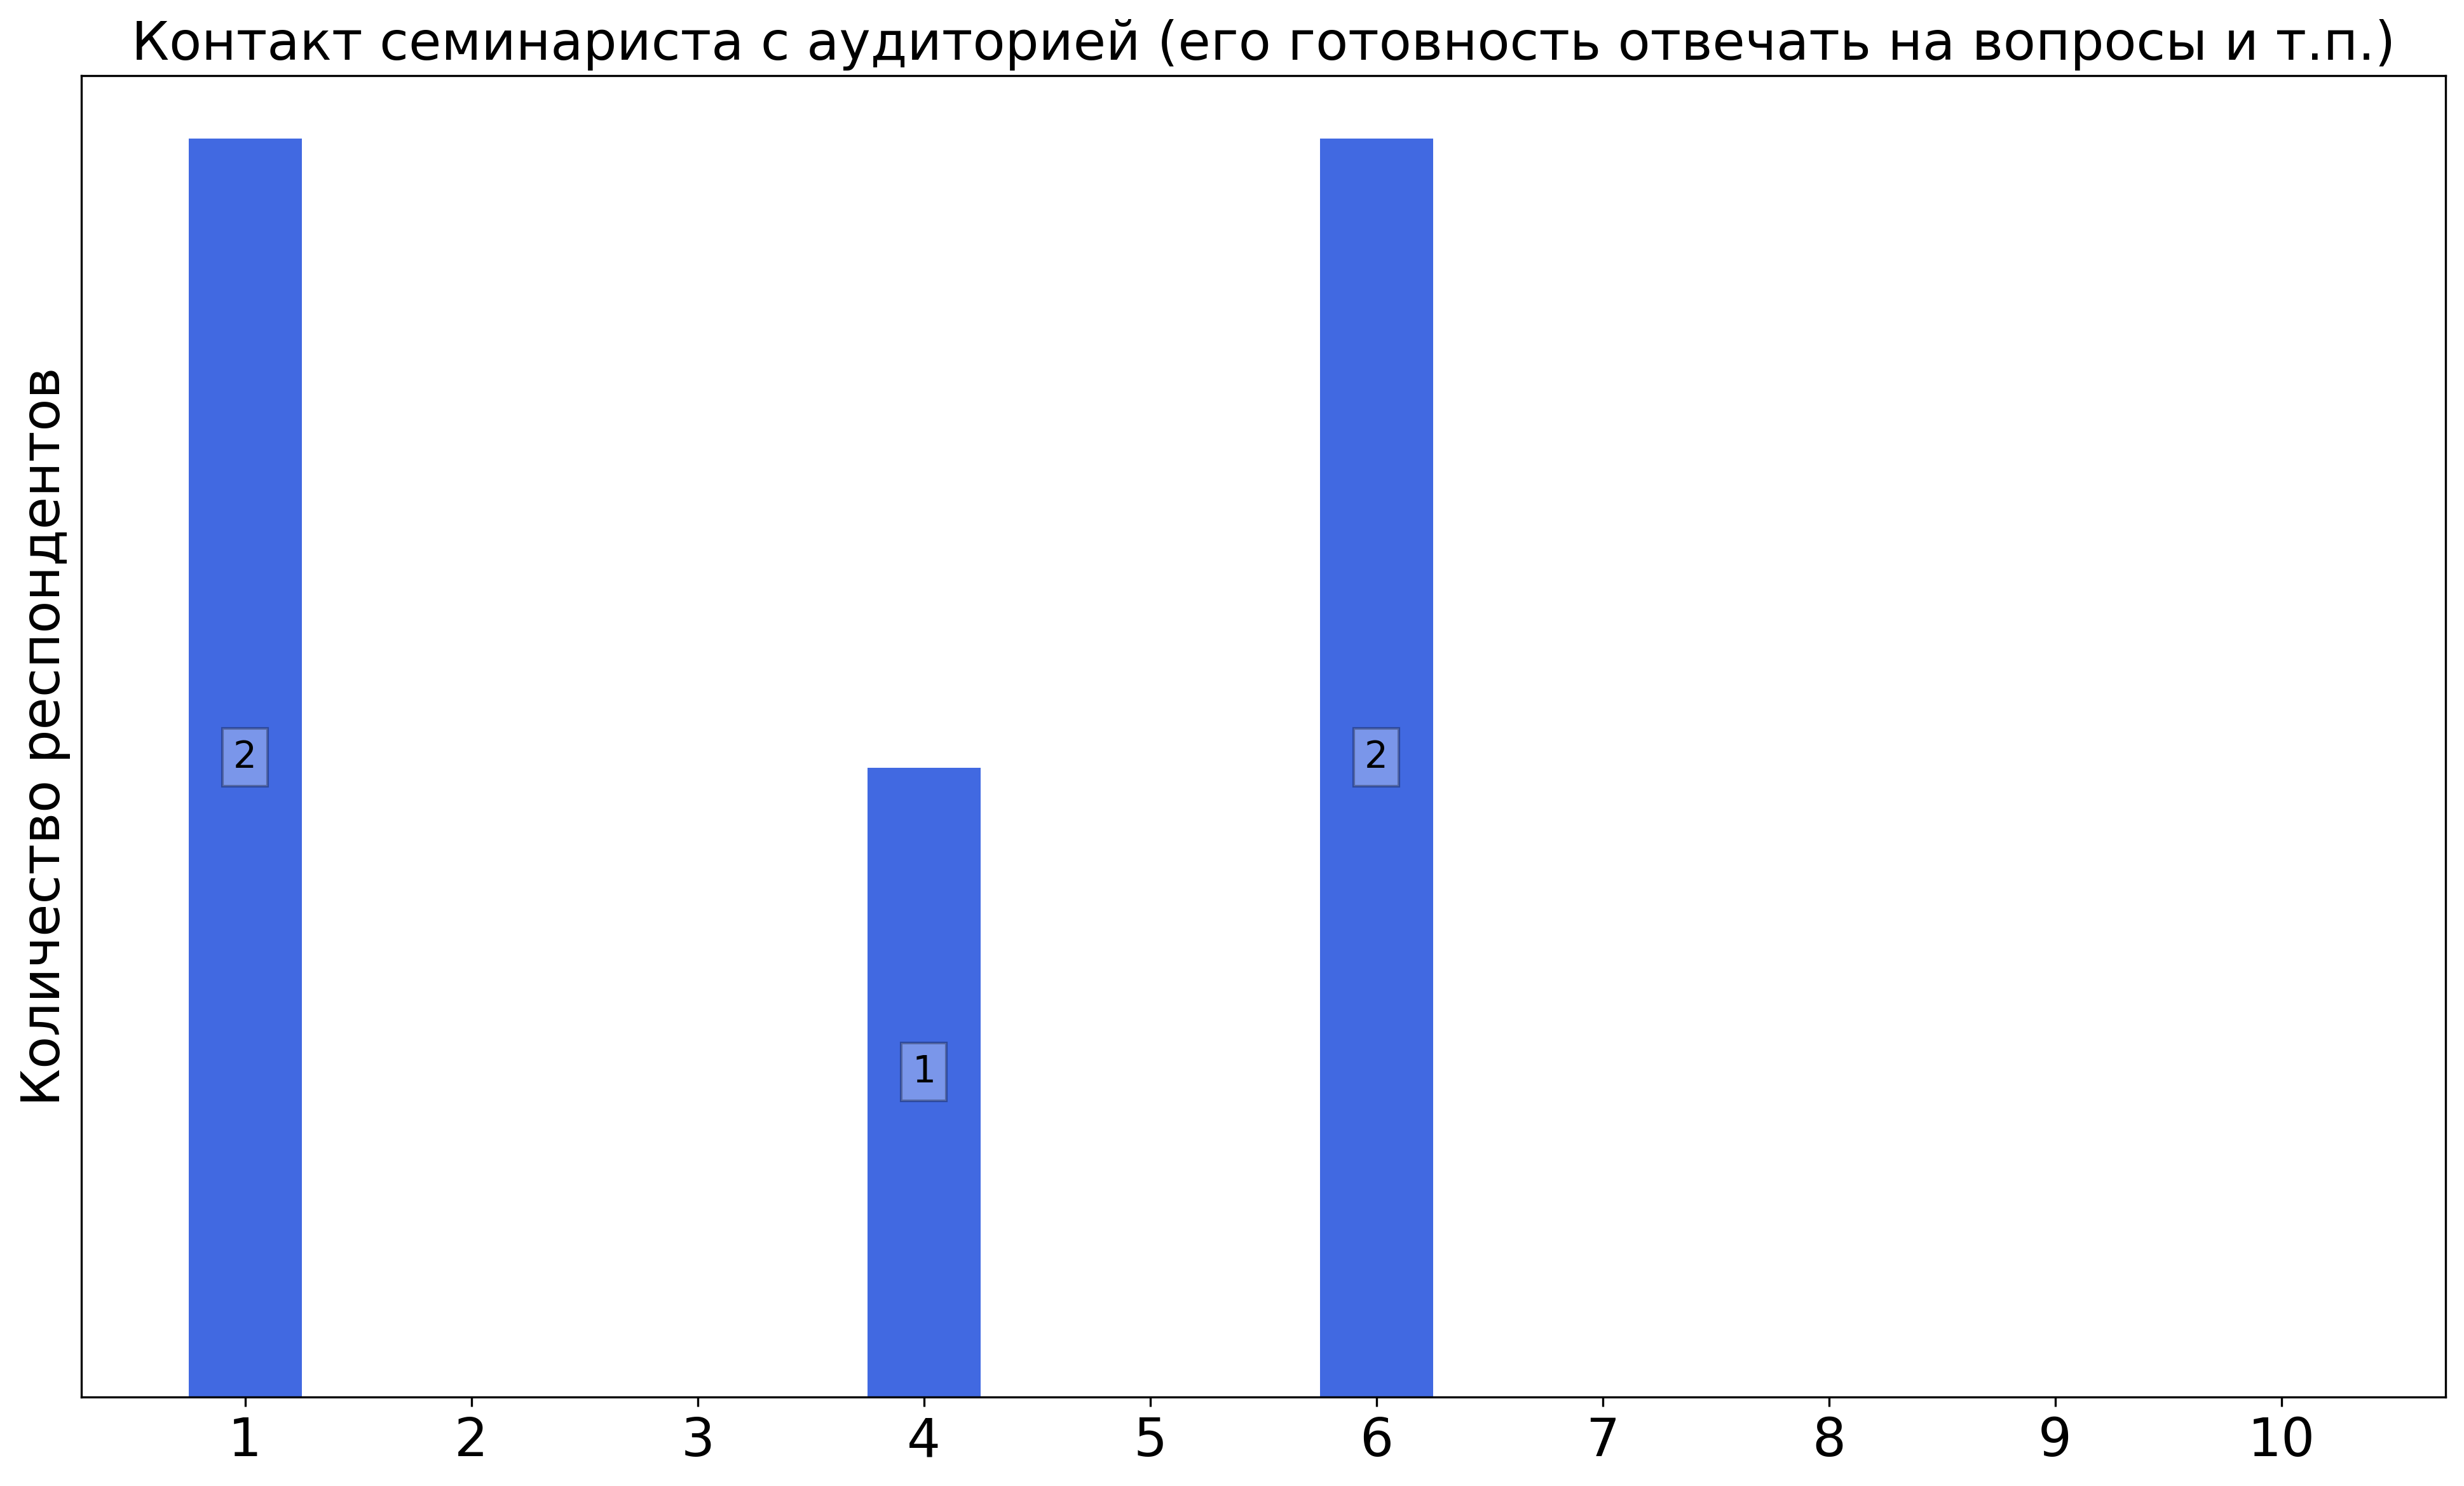
\includegraphics[width=\textwidth]{images/1 course/Общая физика - механика/seminarists-marks-Вановский В.В.-0.png}
			\end{subfigure}
			\begin{subfigure}[b]{0.45\textwidth}
				\centering
				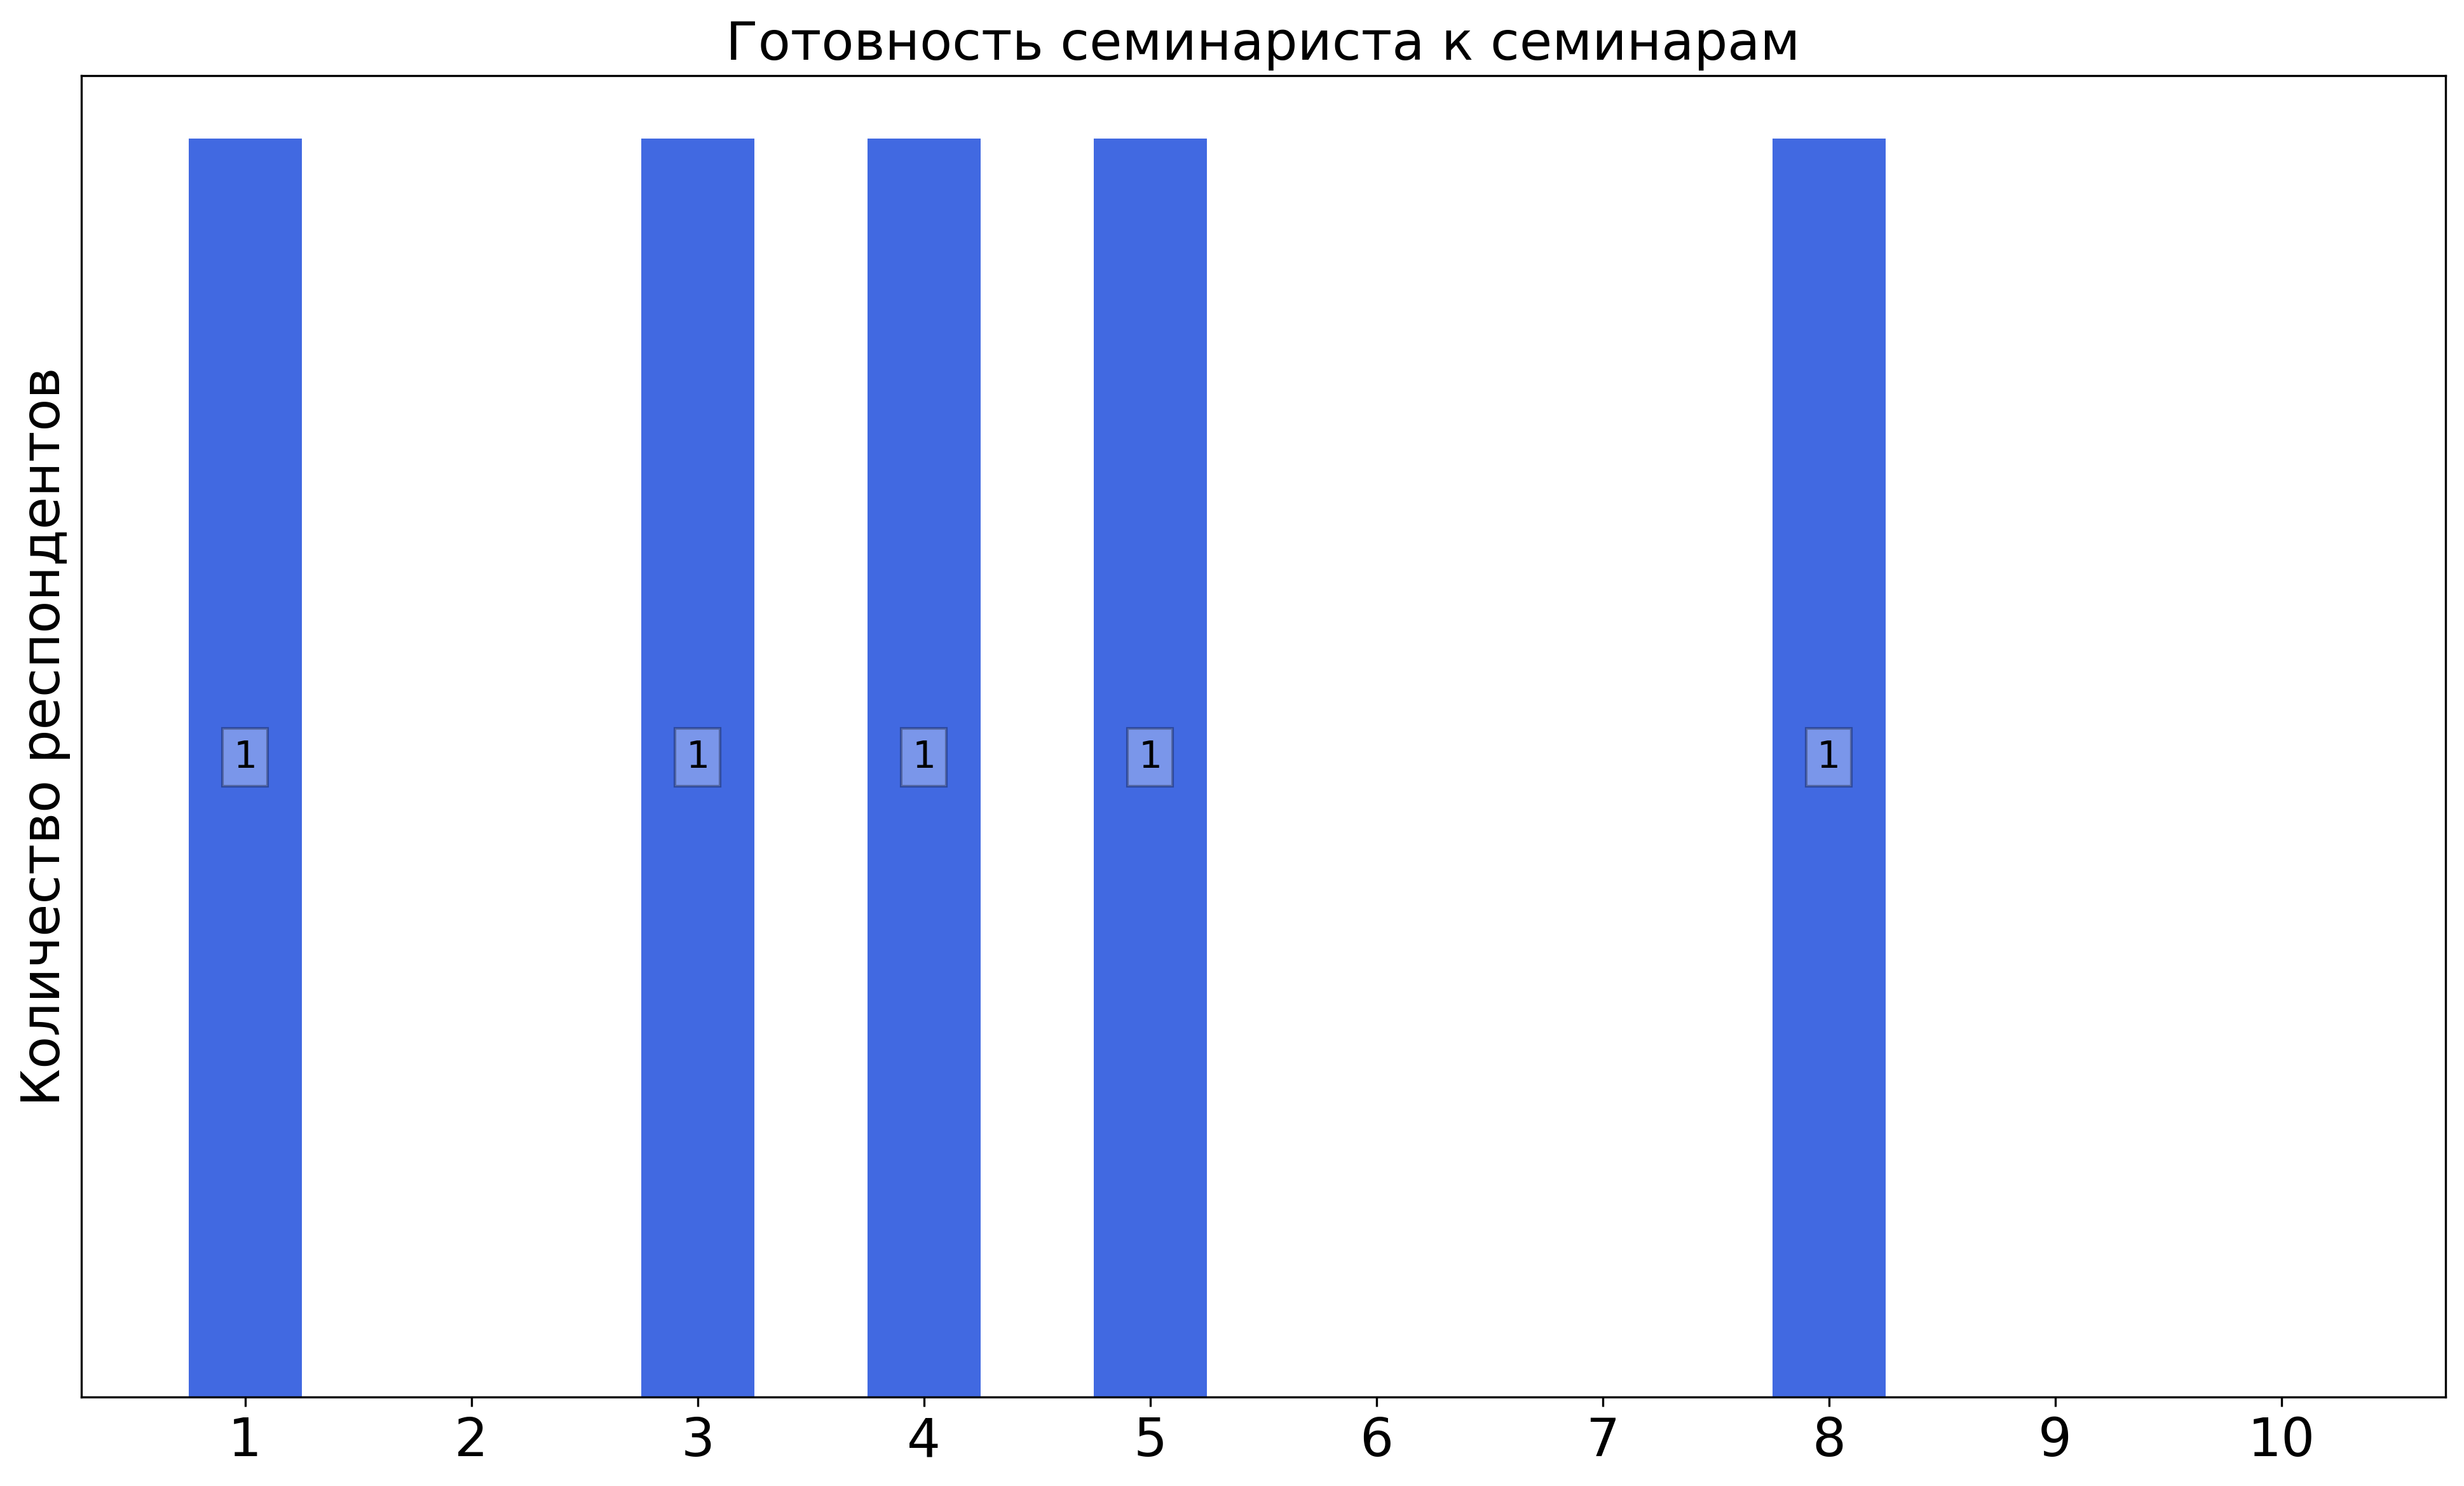
\includegraphics[width=\textwidth]{images/1 course/Общая физика - механика/seminarists-marks-Вановский В.В.-1.png}
			\end{subfigure}
			\begin{subfigure}[b]{0.45\textwidth}
				\centering
				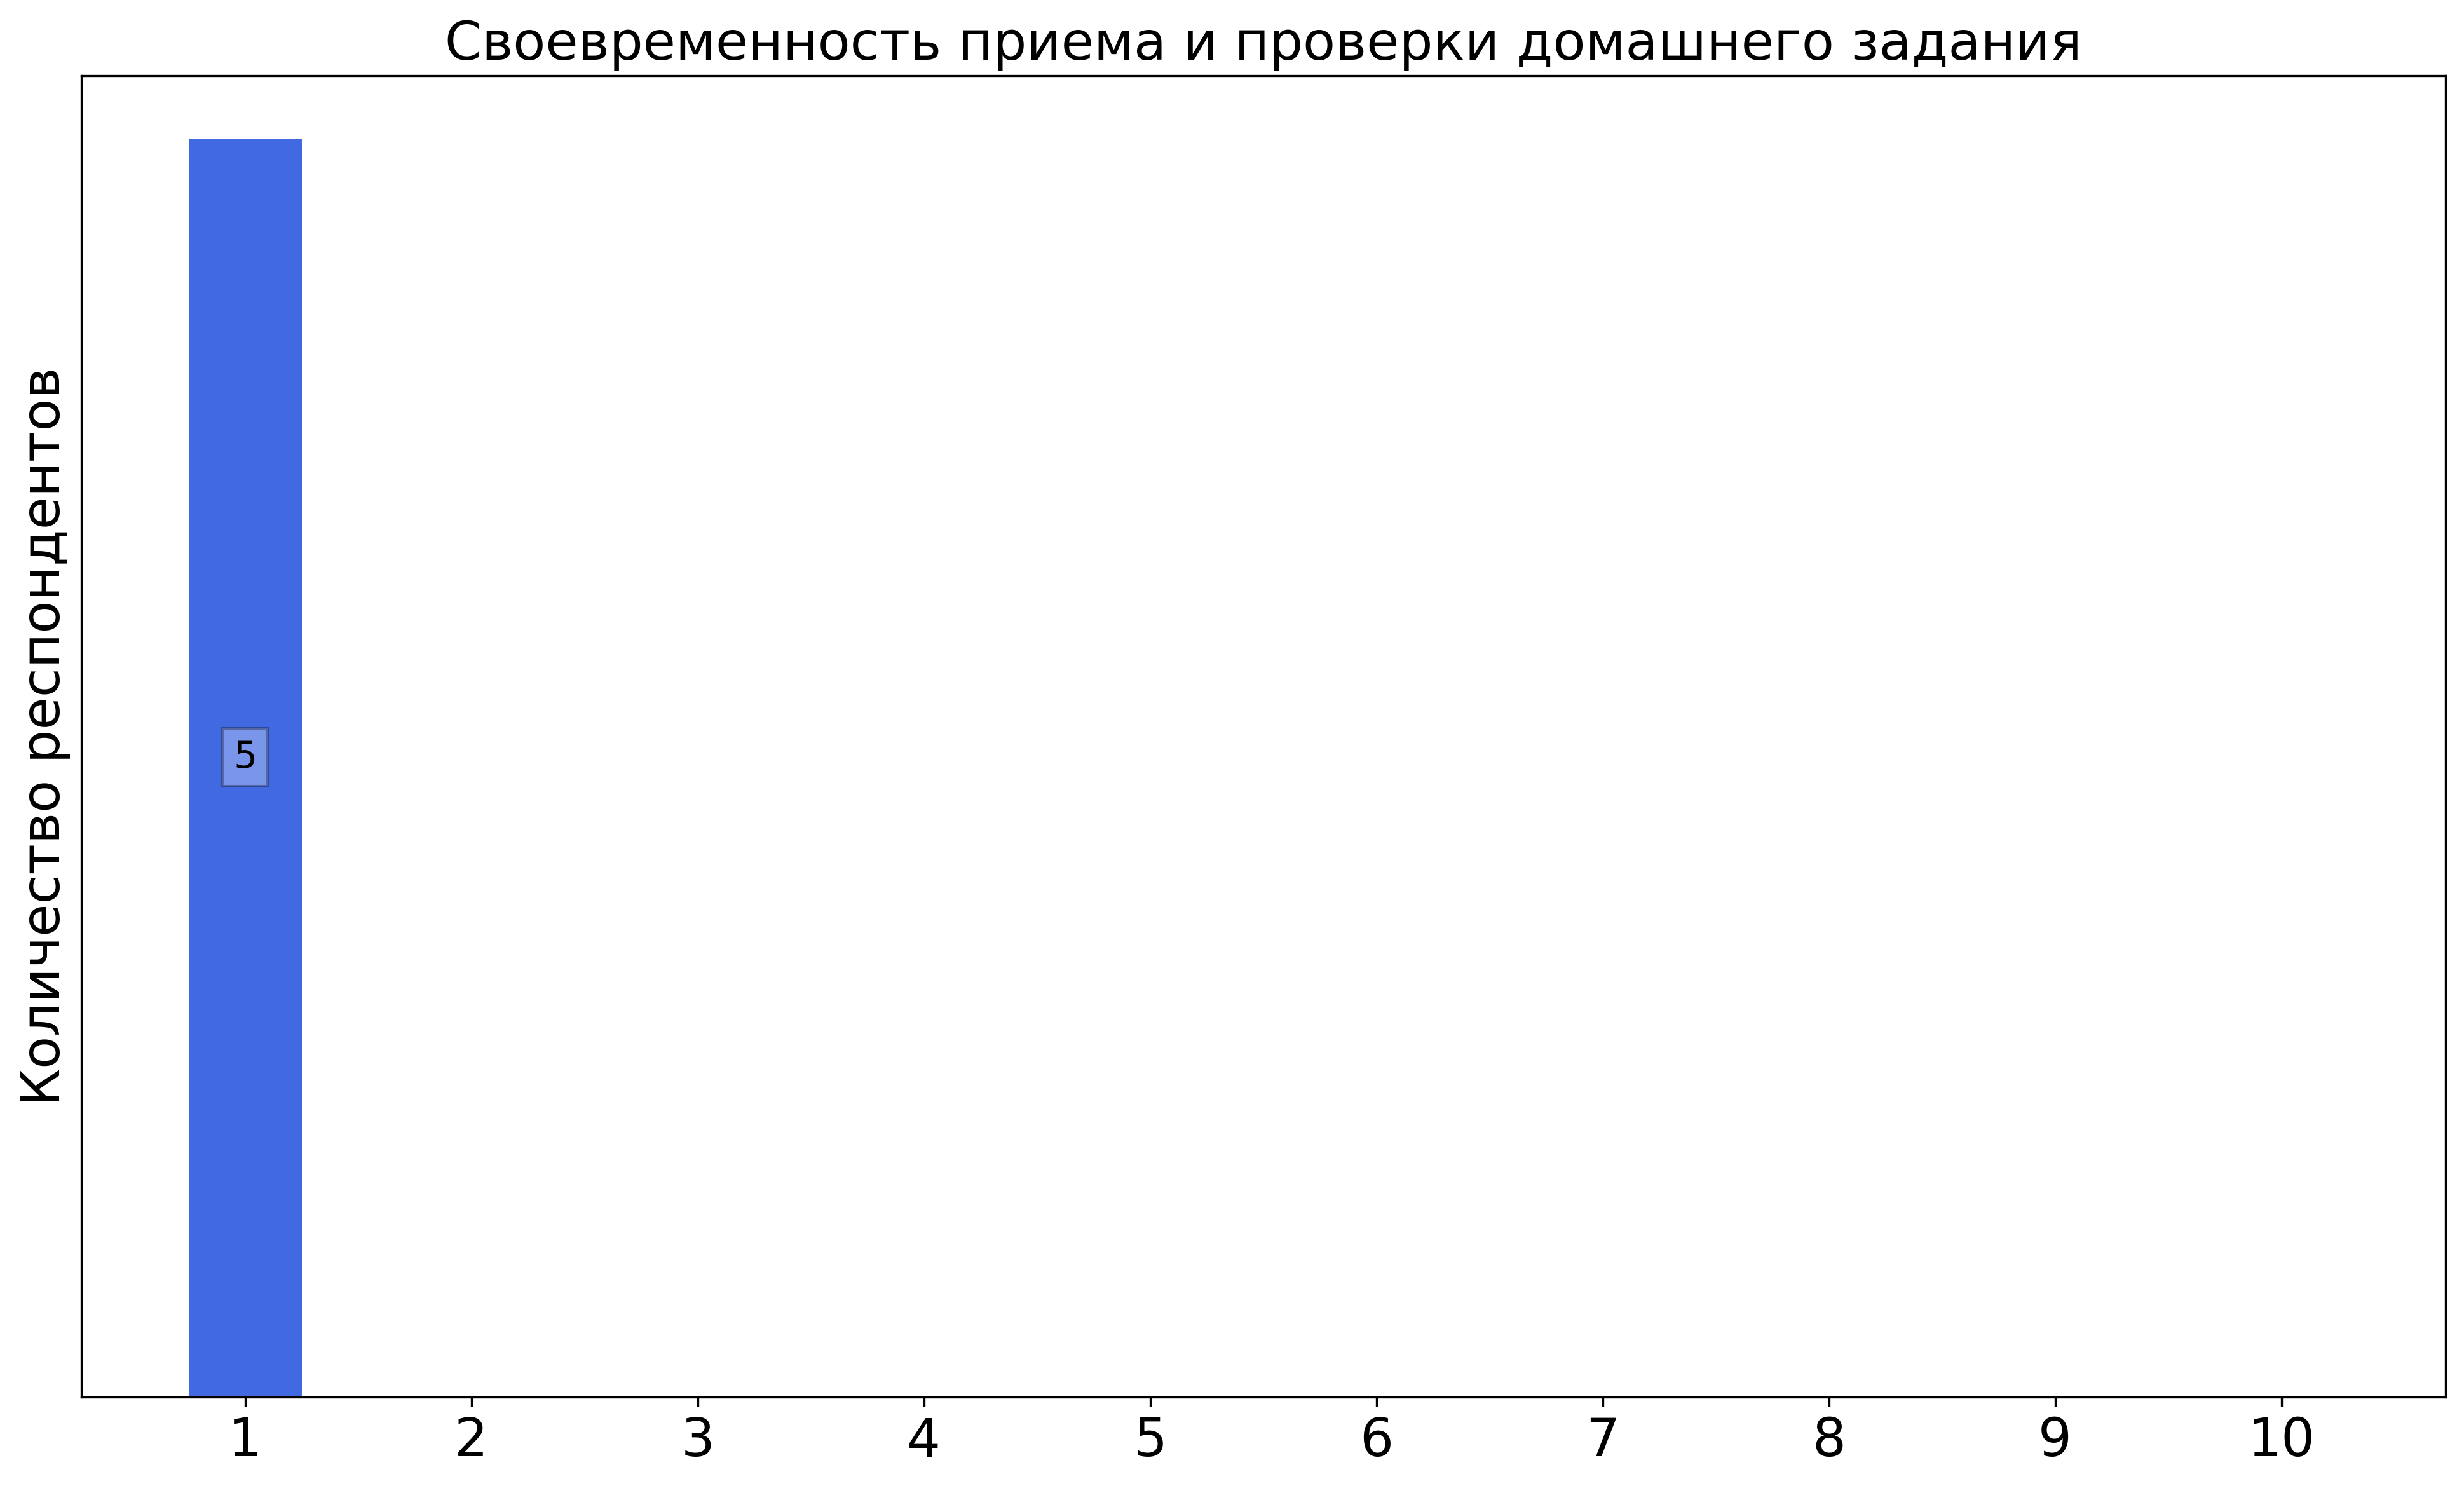
\includegraphics[width=\textwidth]{images/1 course/Общая физика - механика/seminarists-marks-Вановский В.В.-2.png}
			\end{subfigure}
			\begin{subfigure}[b]{0.45\textwidth}
				\centering
				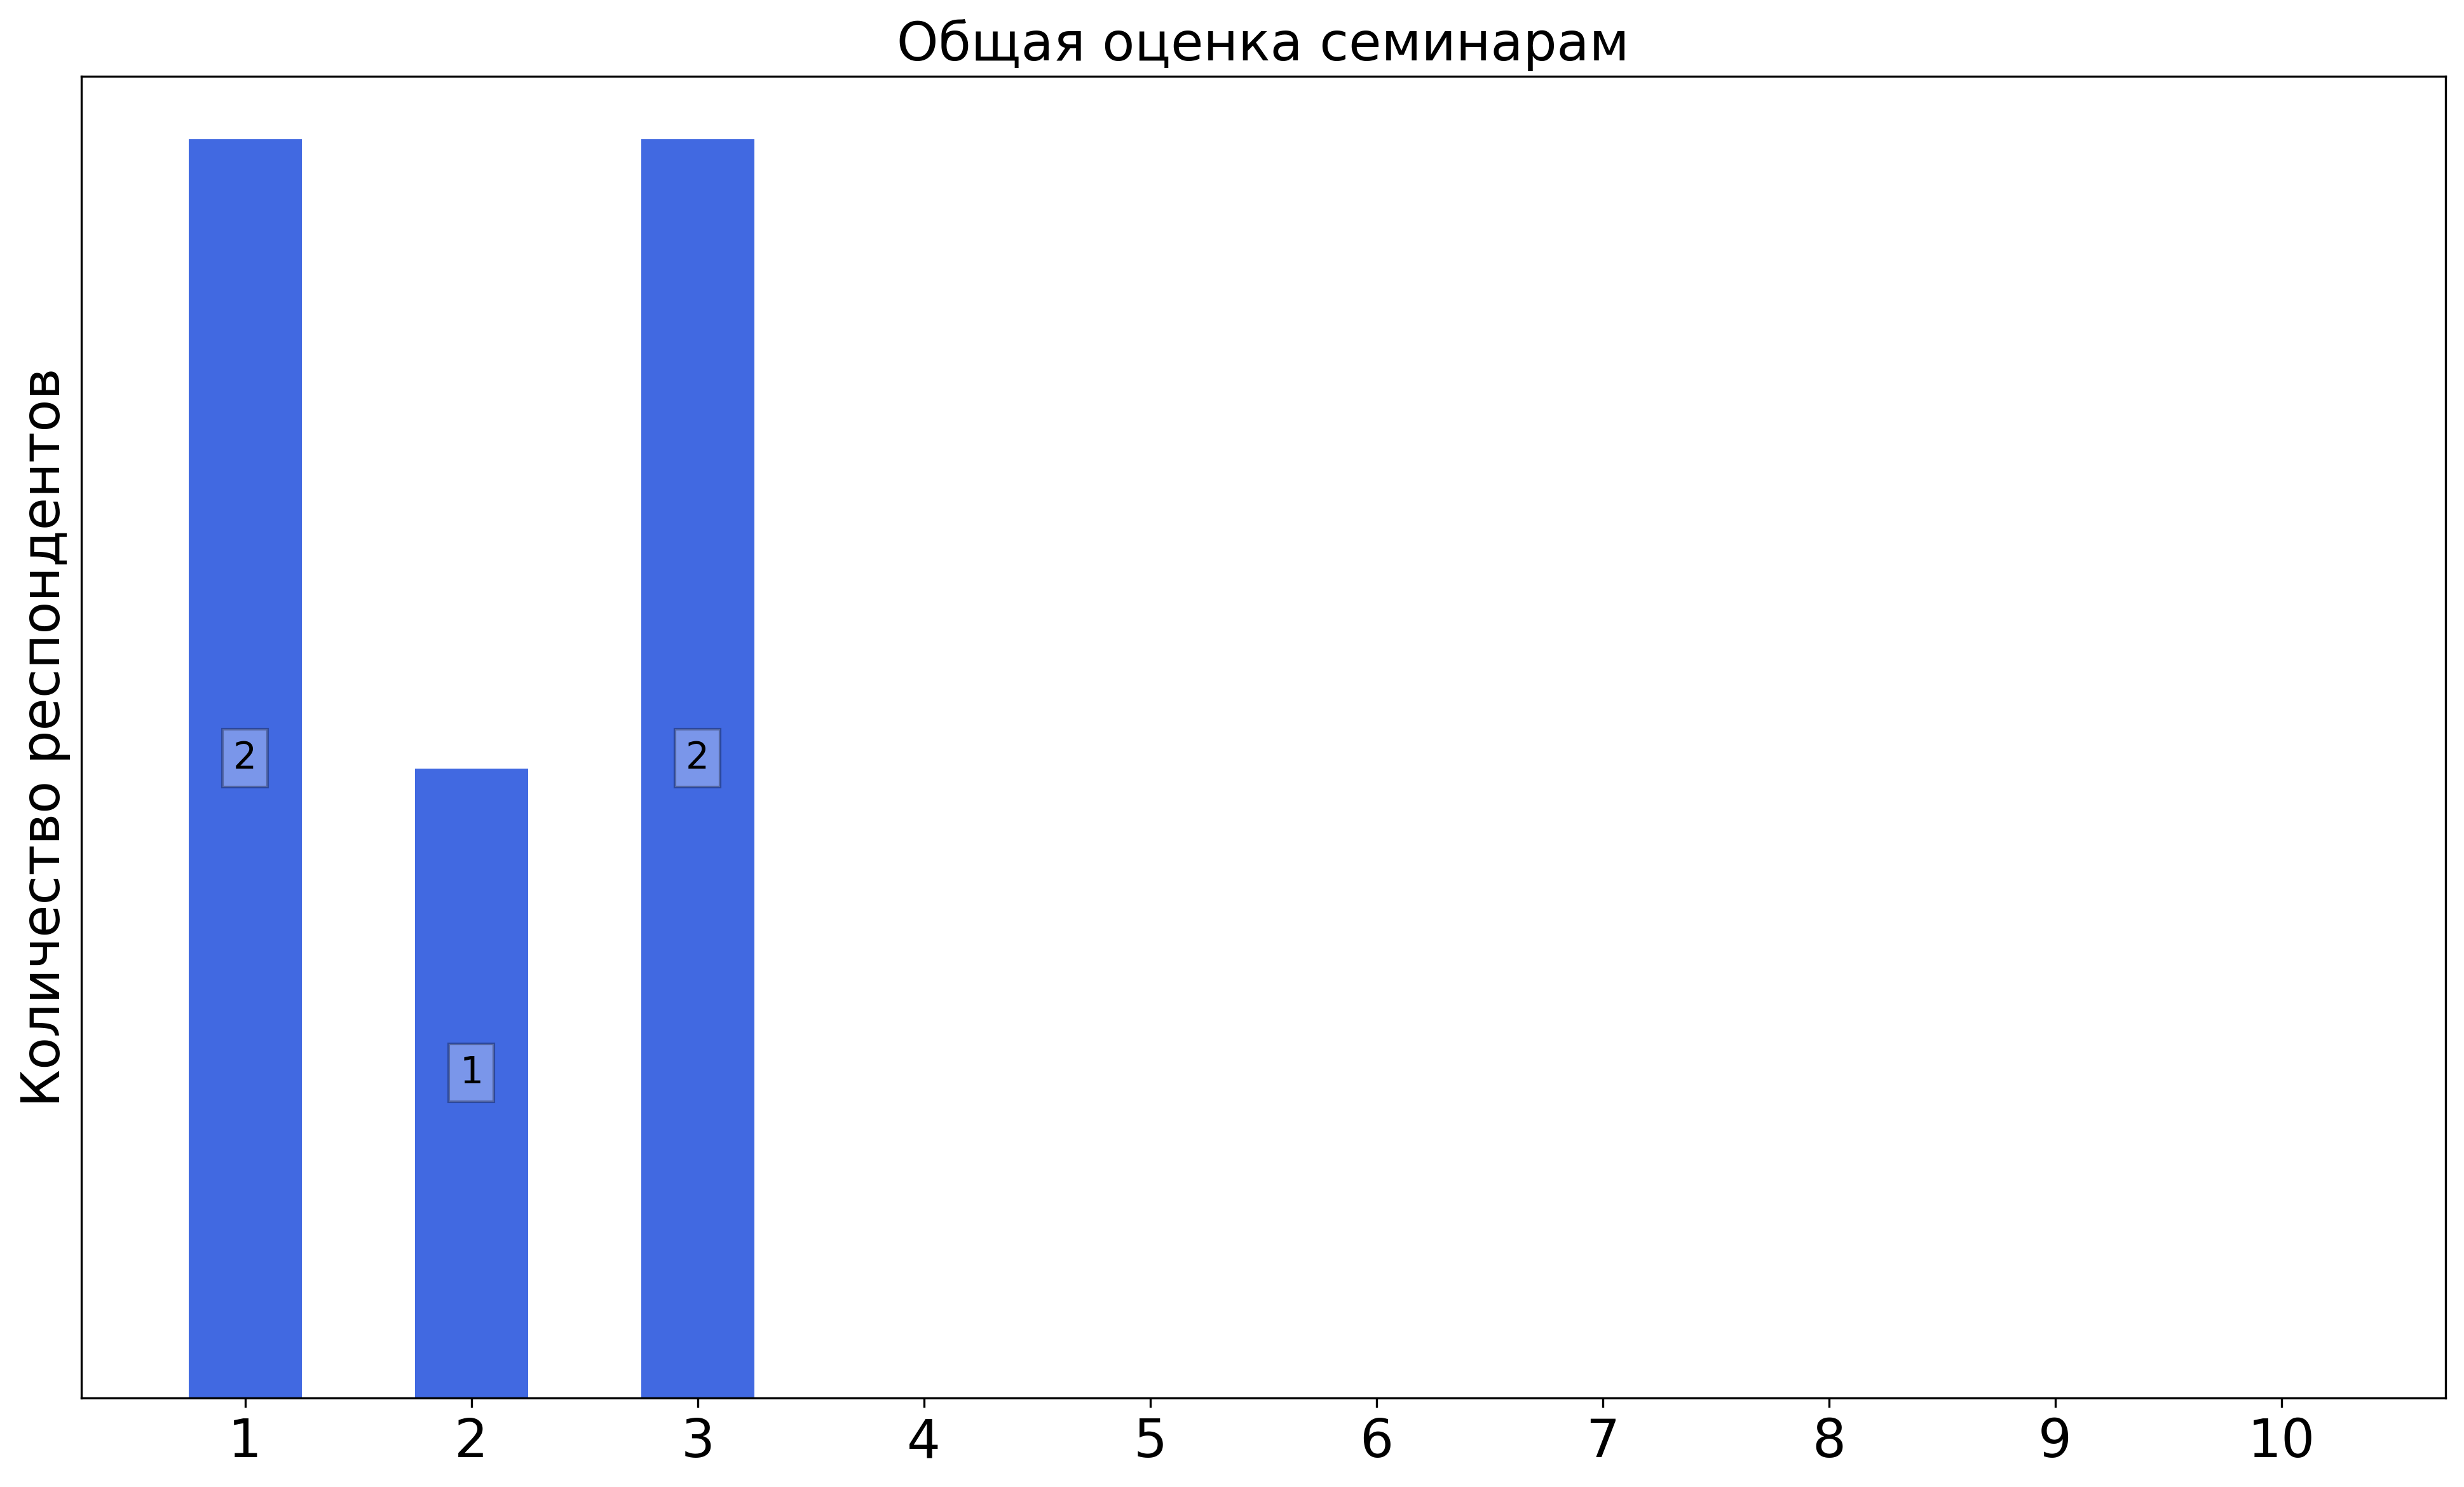
\includegraphics[width=\textwidth]{images/1 course/Общая физика - механика/seminarists-marks-Вановский В.В.-3.png}
			\end{subfigure}	
			\caption{Оценки респондентов о качестве преподавания семинаров}
		\end{figure}

		\textbf{Комментарии студентов о семинаристе\protect\footnote{сохранены оригинальные орфография и пунктуация}}
        \begin{commentbox} 
            Объясняет очень быстро и непонятно, кроме того, сразу видно, что преподавателю абсолютно безразличны студенты, которых он учит. Когда он видит непонимающие глаза студентов, говорит примерно следующее: ну я запутал вас ребята, ничего когда-нибудь научитесь. Разговаривая со студентами или объясняя материал, смотрит в пол. Не признает свои ошибки: не поднял баллы за семестровую контрольную, в которой на самом деле не было вычислительной ошибки, как он думал ранее. Свое решение он оправдал так: ну я же должен был за что то снять. При всем этом оценивает достаточно строго. Если человек не сделал все задание, идешь на экзамен с -3 баллами. По 2 заданию  дал контрольную выше уровня письменного экзамена  из 5 заданий на 1.5 часа, в итоге никому выше хор за задания не поставил. В этой контрольной было задание, требующее мат. аппарат из 2 семестра. Он это прокомментировал так: ну никого не волнует что у вас этого не было. Назначил сдачу заданий через полчаса после окончания письменного экзамена по мат.анализу, сказав, что "письмак мы за 1.5 часа должны написать, там задания ни о чем". Задания проверяет очень долго, узнали оценку непосредственно перед самим устным экзаменом по физике. Обратная связь со студентами отсутствует совсем. Очень долго отвечает на сообщения: неделями, месяцами, а иногда попросту игнорирует.
        \end{commentbox} 
       
        \begin{commentbox} 
            По моему мнению, Вановский - очень плохой семинарист. Материал, который он рассказывает, понятен очень посредственно, несмотря на то, что я очень много задавал вопросов, а каждый семинар по сути приходит к тому, что он говорит: "Ребят, кажется я вас запутал". Дз фактически не проверяет(о чем он даже даже говорил в итоге), а ставит по его контрольным, которые сложнее письмака, а дается варик на 5 задач на 1,5 часа, по которым он оценивает. Если ему ПОКАЗАЛОСЬ, что ты мог списать какую-нибудл задачу/плохо написал его кр, то он устроит тебе доп сдачу на часа 4 сразу после письмака по матану, где нужно решать его щадачи, чтобы просто не получить -3 за дз(а такие люди в итоге были). Игнорит все сообщения в личке, которую сам дал нам, куда он просил скидывать дз, в том числе с вопросами, когда он проверит дз(оценки он нам озвучил в итоге в вечер перед устным экзом). То, что он по сути не будет проверять дз(а за несколько минут от момента прочитывания моих сообщений со всеми фотками дз до оглашения всех оценок за дз он не мог его проверить) , он не говорил. Письмак я нормально написал лишь за счет того, что ходил к другому семеру + посещал доп семы Овчинкина(несмотря на то, что ни один семинар Вановского я не пропустил). Он плохо ведет семинары, жестит по оцениванию «дз» и в целом у него отношение к ведению занятий достаточно пофигистическое.  
        \end{commentbox} 
       
        \begin{commentbox}
            Разборы задач часто остаются непонятными даже спустя несколько вопросов. Также домашнее задание проверяется очень долго, даже неизвестно, проверено ли дз до конца за прошлый семестр. Оценка за задание выставляется по каким-то другим критериям, а не по сделанному задавальнику 
        \end{commentbox} 
				

	\subsubsection{Отзыв студентов о семинарах. Семинарист: Лилиенберг И.В.}		
		\begin{figure}[H]
			\centering
			\begin{subfigure}[b]{0.45\textwidth}
				\centering
				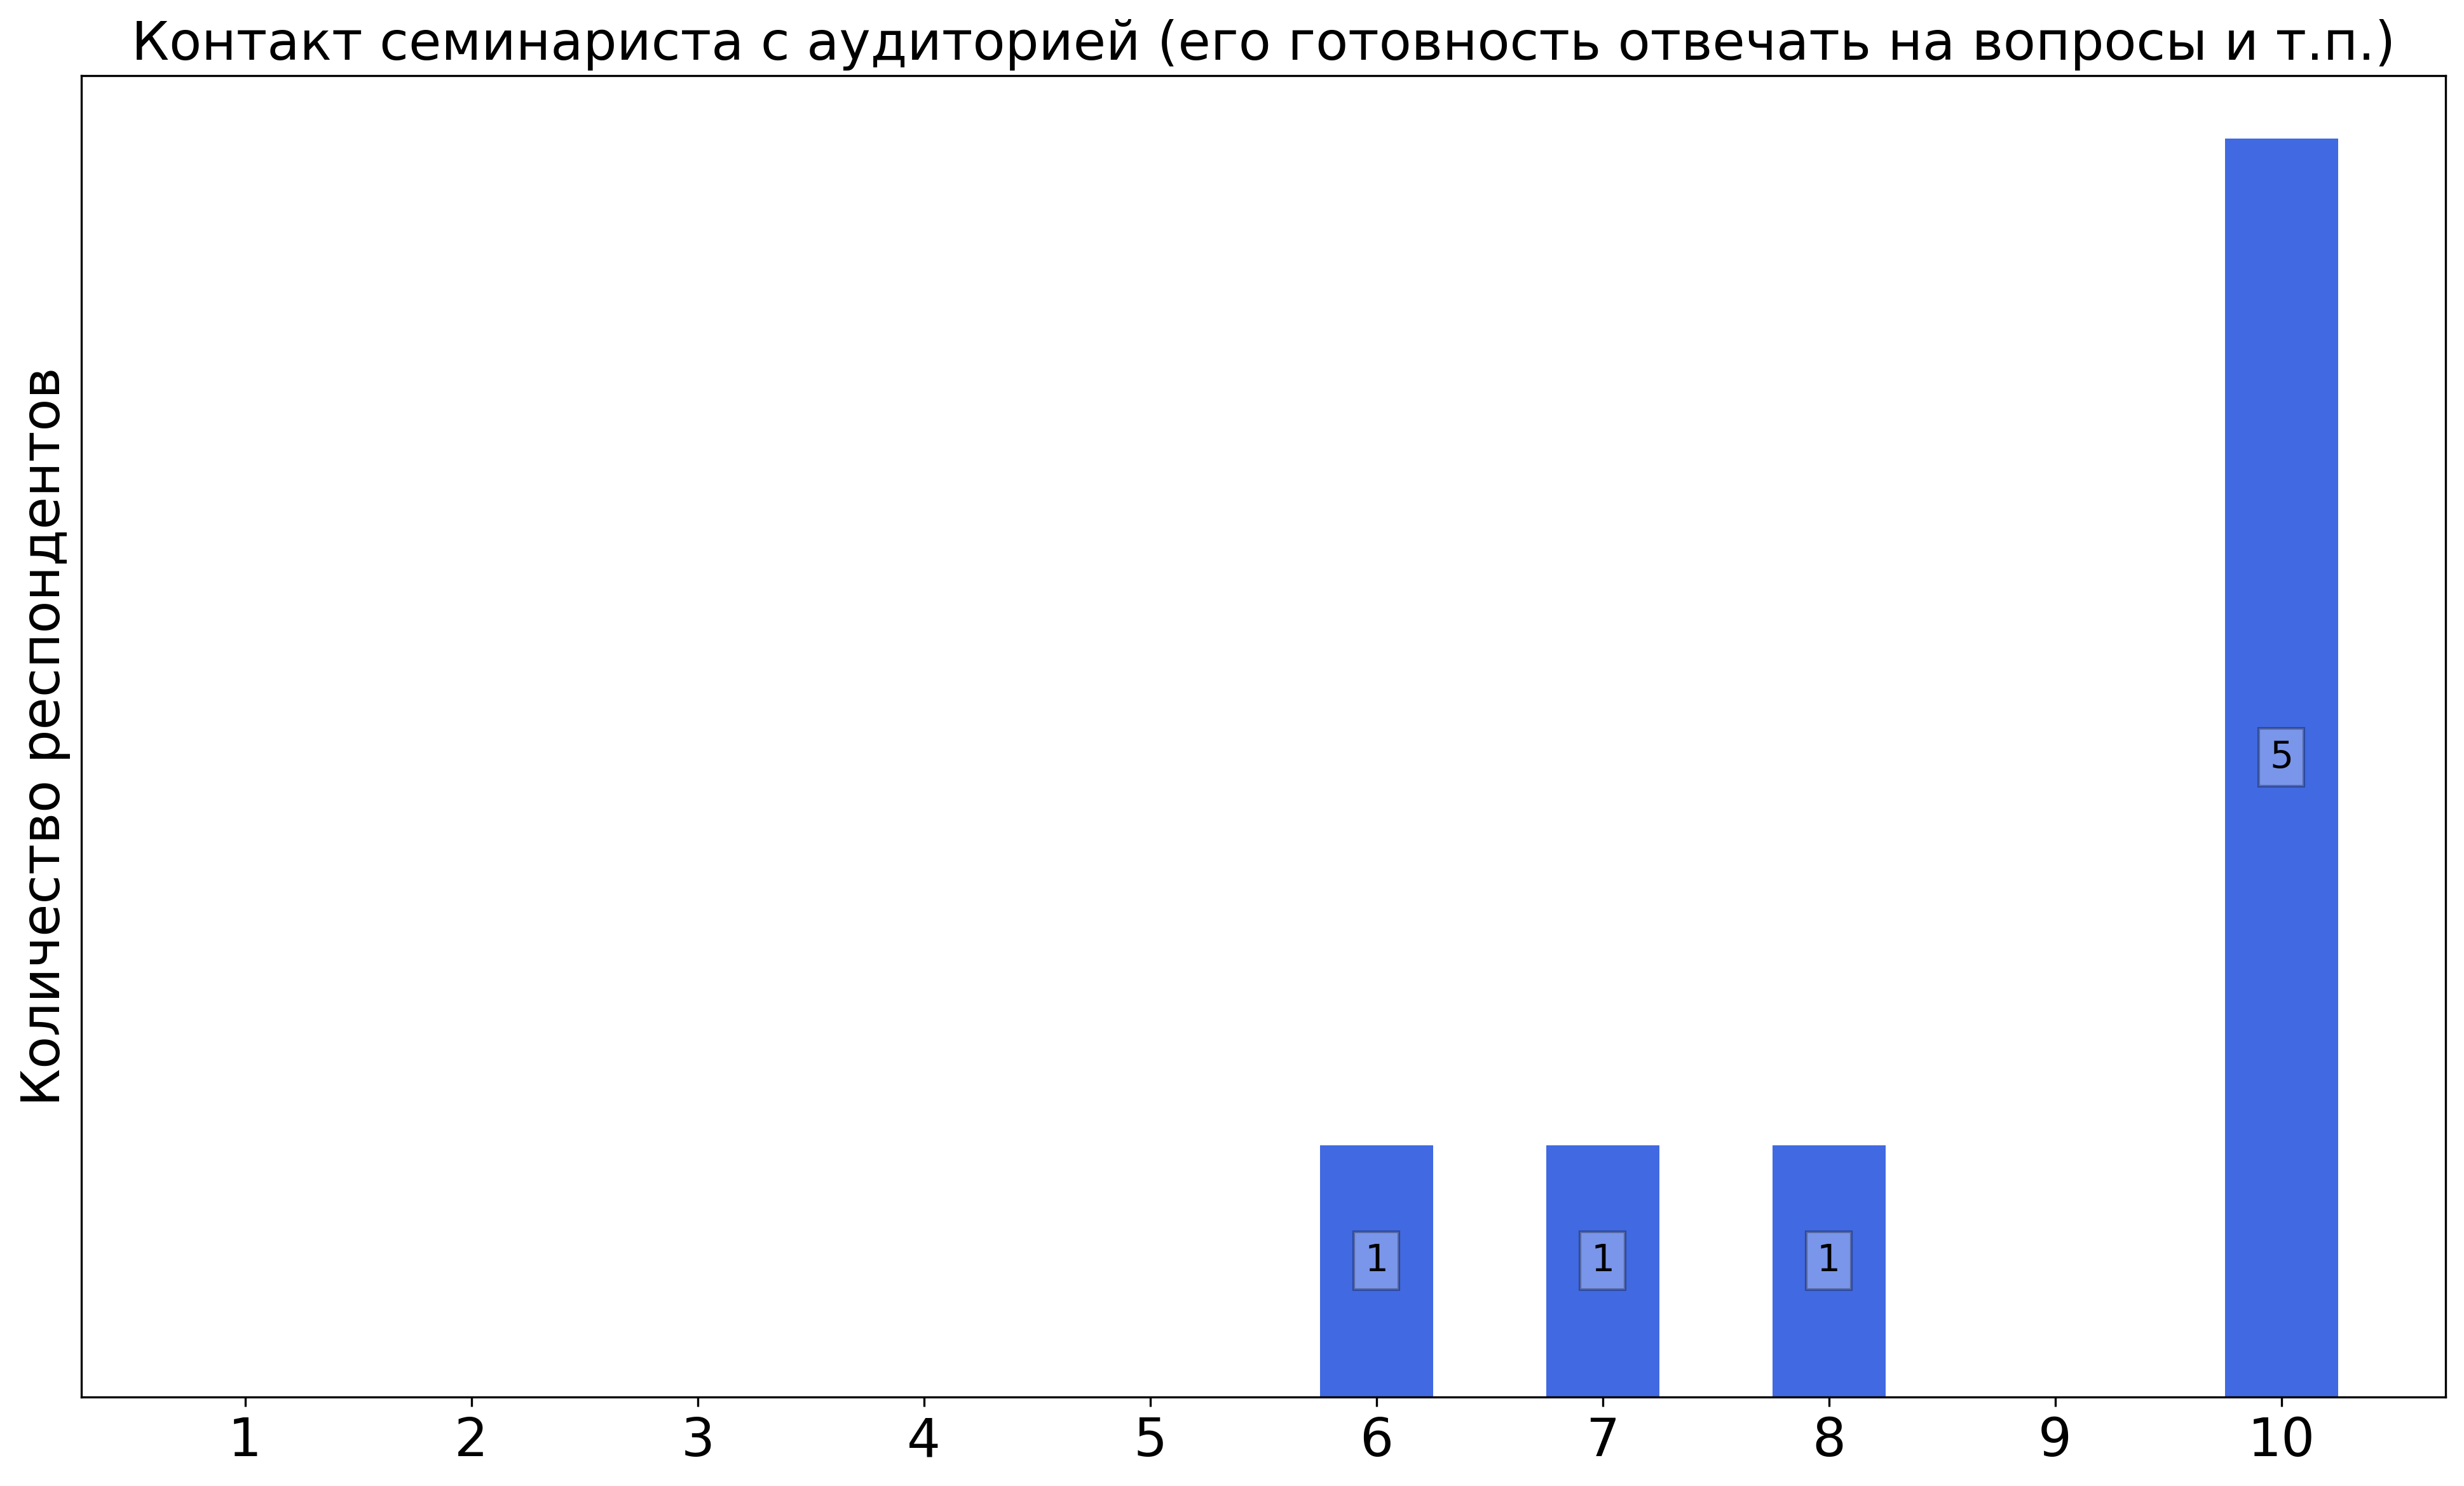
\includegraphics[width=\textwidth]{images/1 course/Общая физика - механика/seminarists-marks-Лилиенберг И.В.-0.png}
			\end{subfigure}
			\begin{subfigure}[b]{0.45\textwidth}
				\centering
				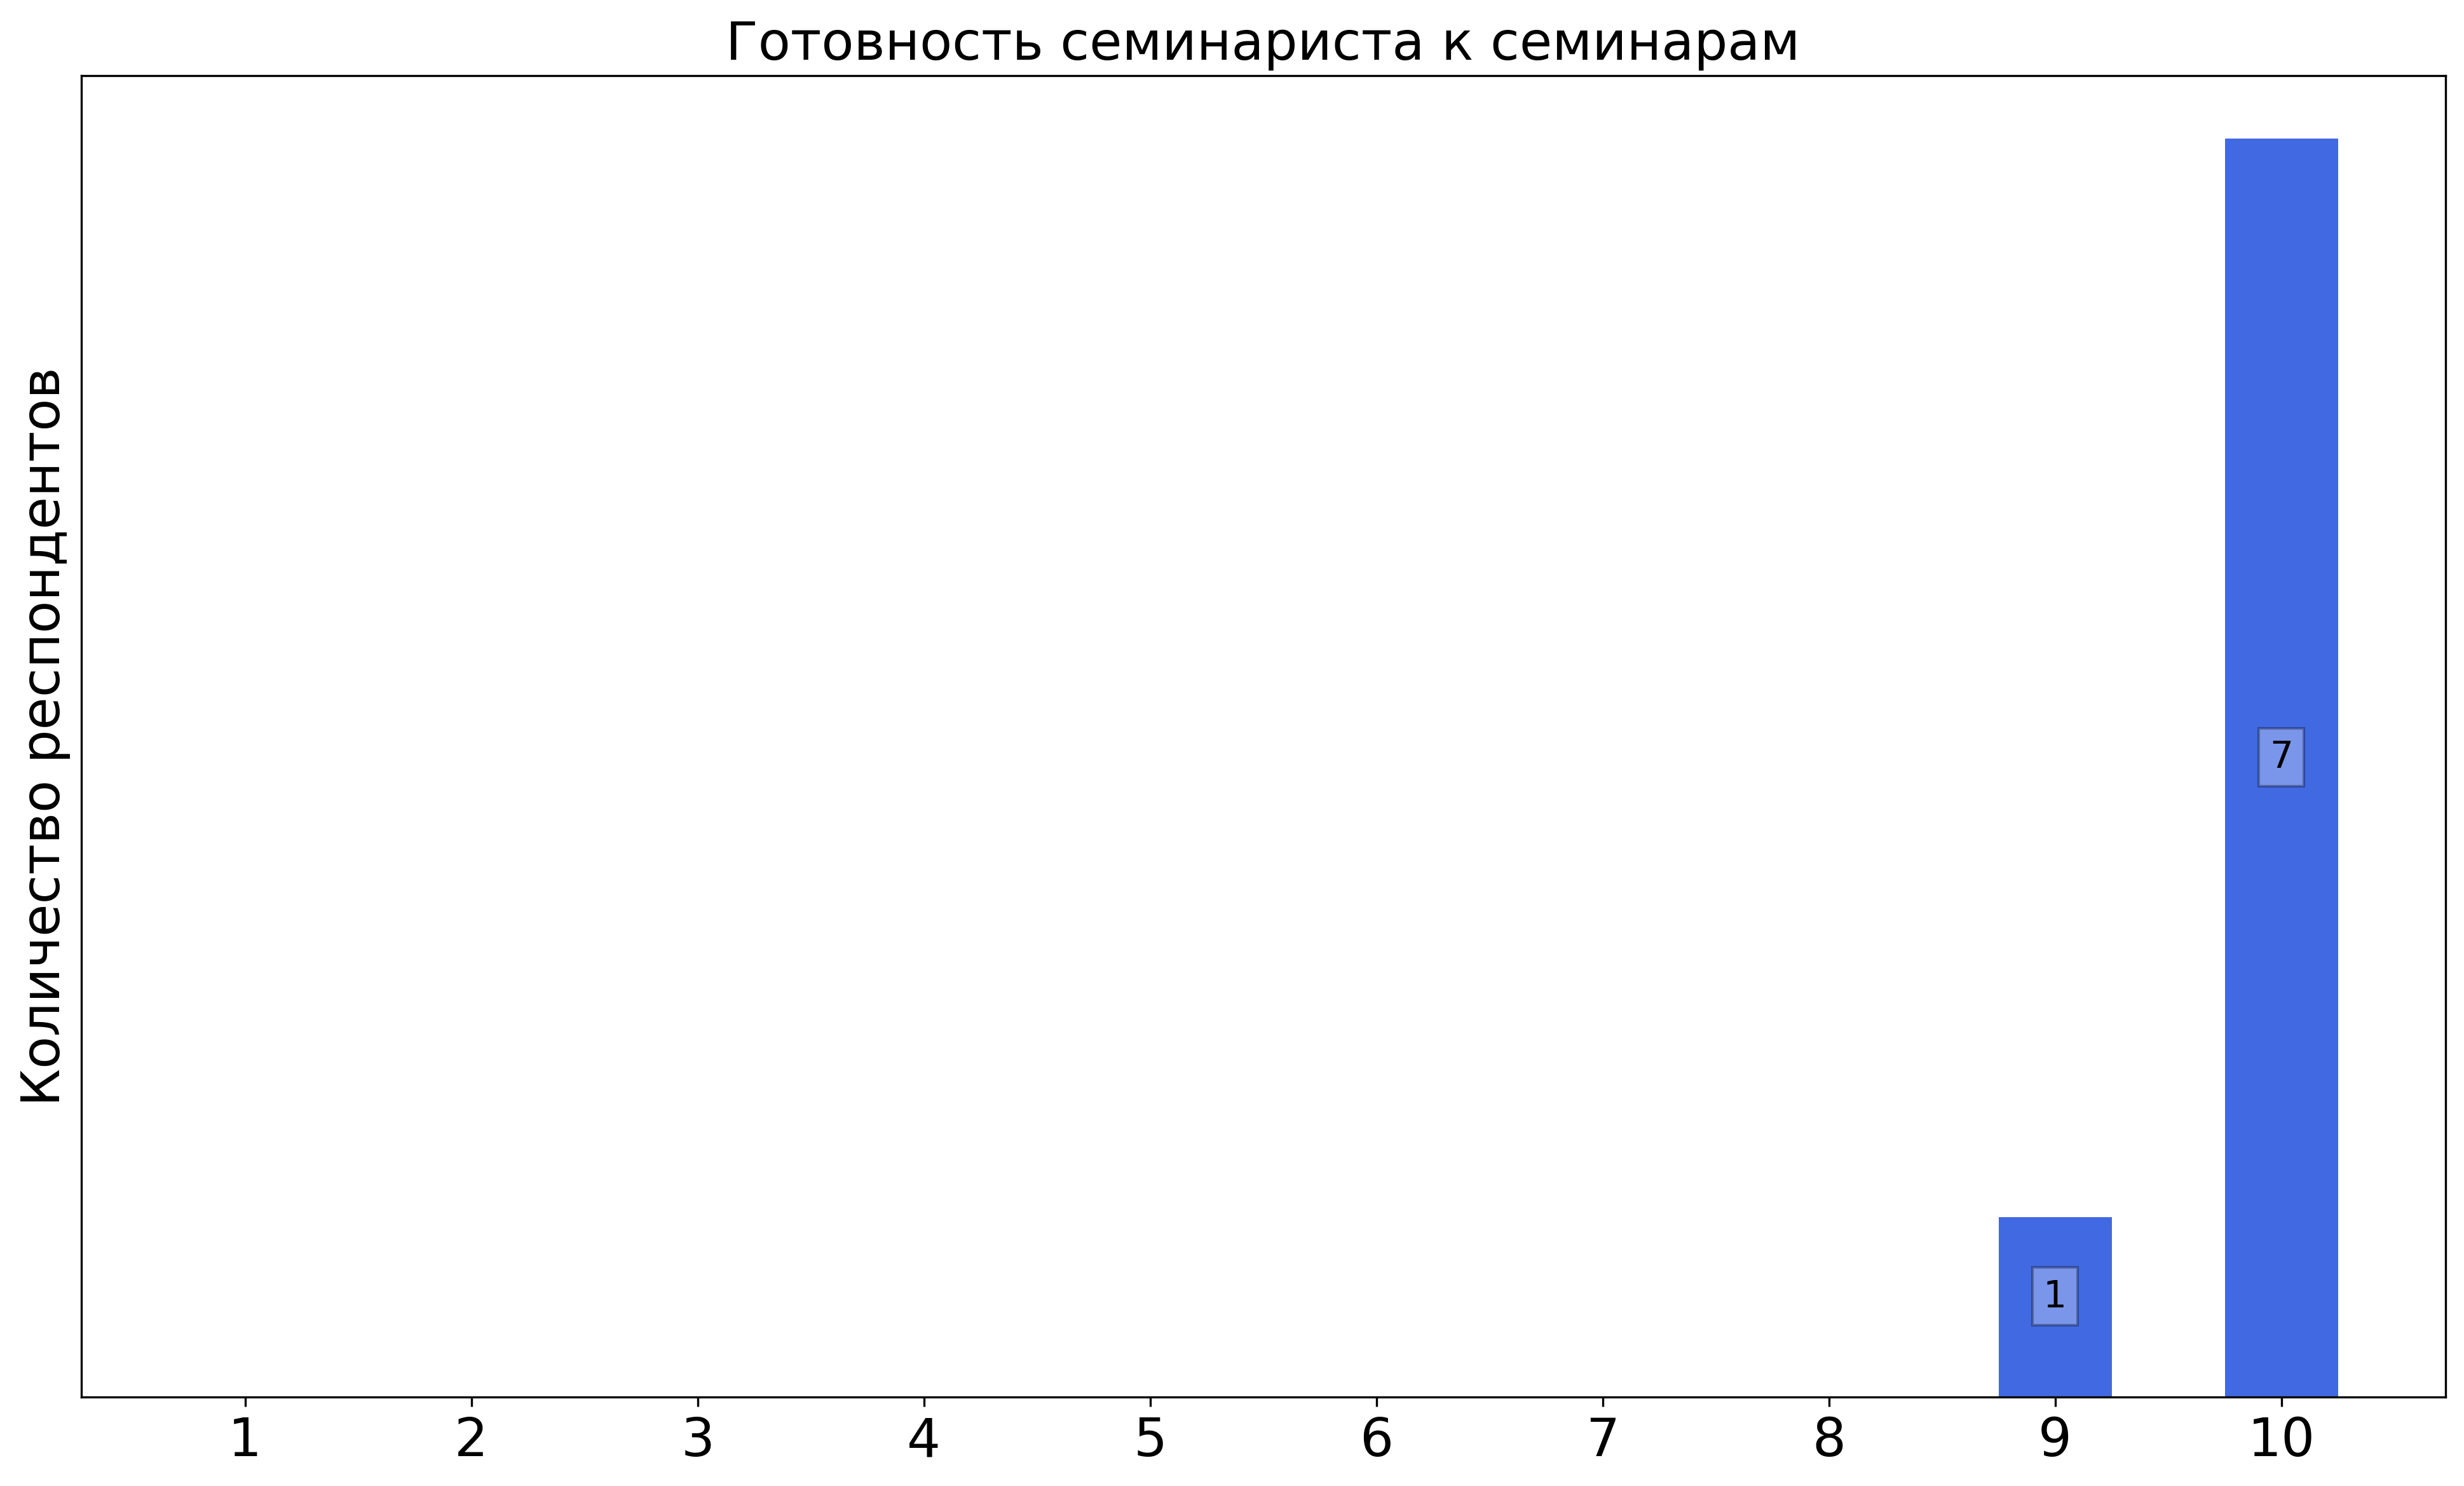
\includegraphics[width=\textwidth]{images/1 course/Общая физика - механика/seminarists-marks-Лилиенберг И.В.-1.png}
			\end{subfigure}
			\begin{subfigure}[b]{0.45\textwidth}
				\centering
				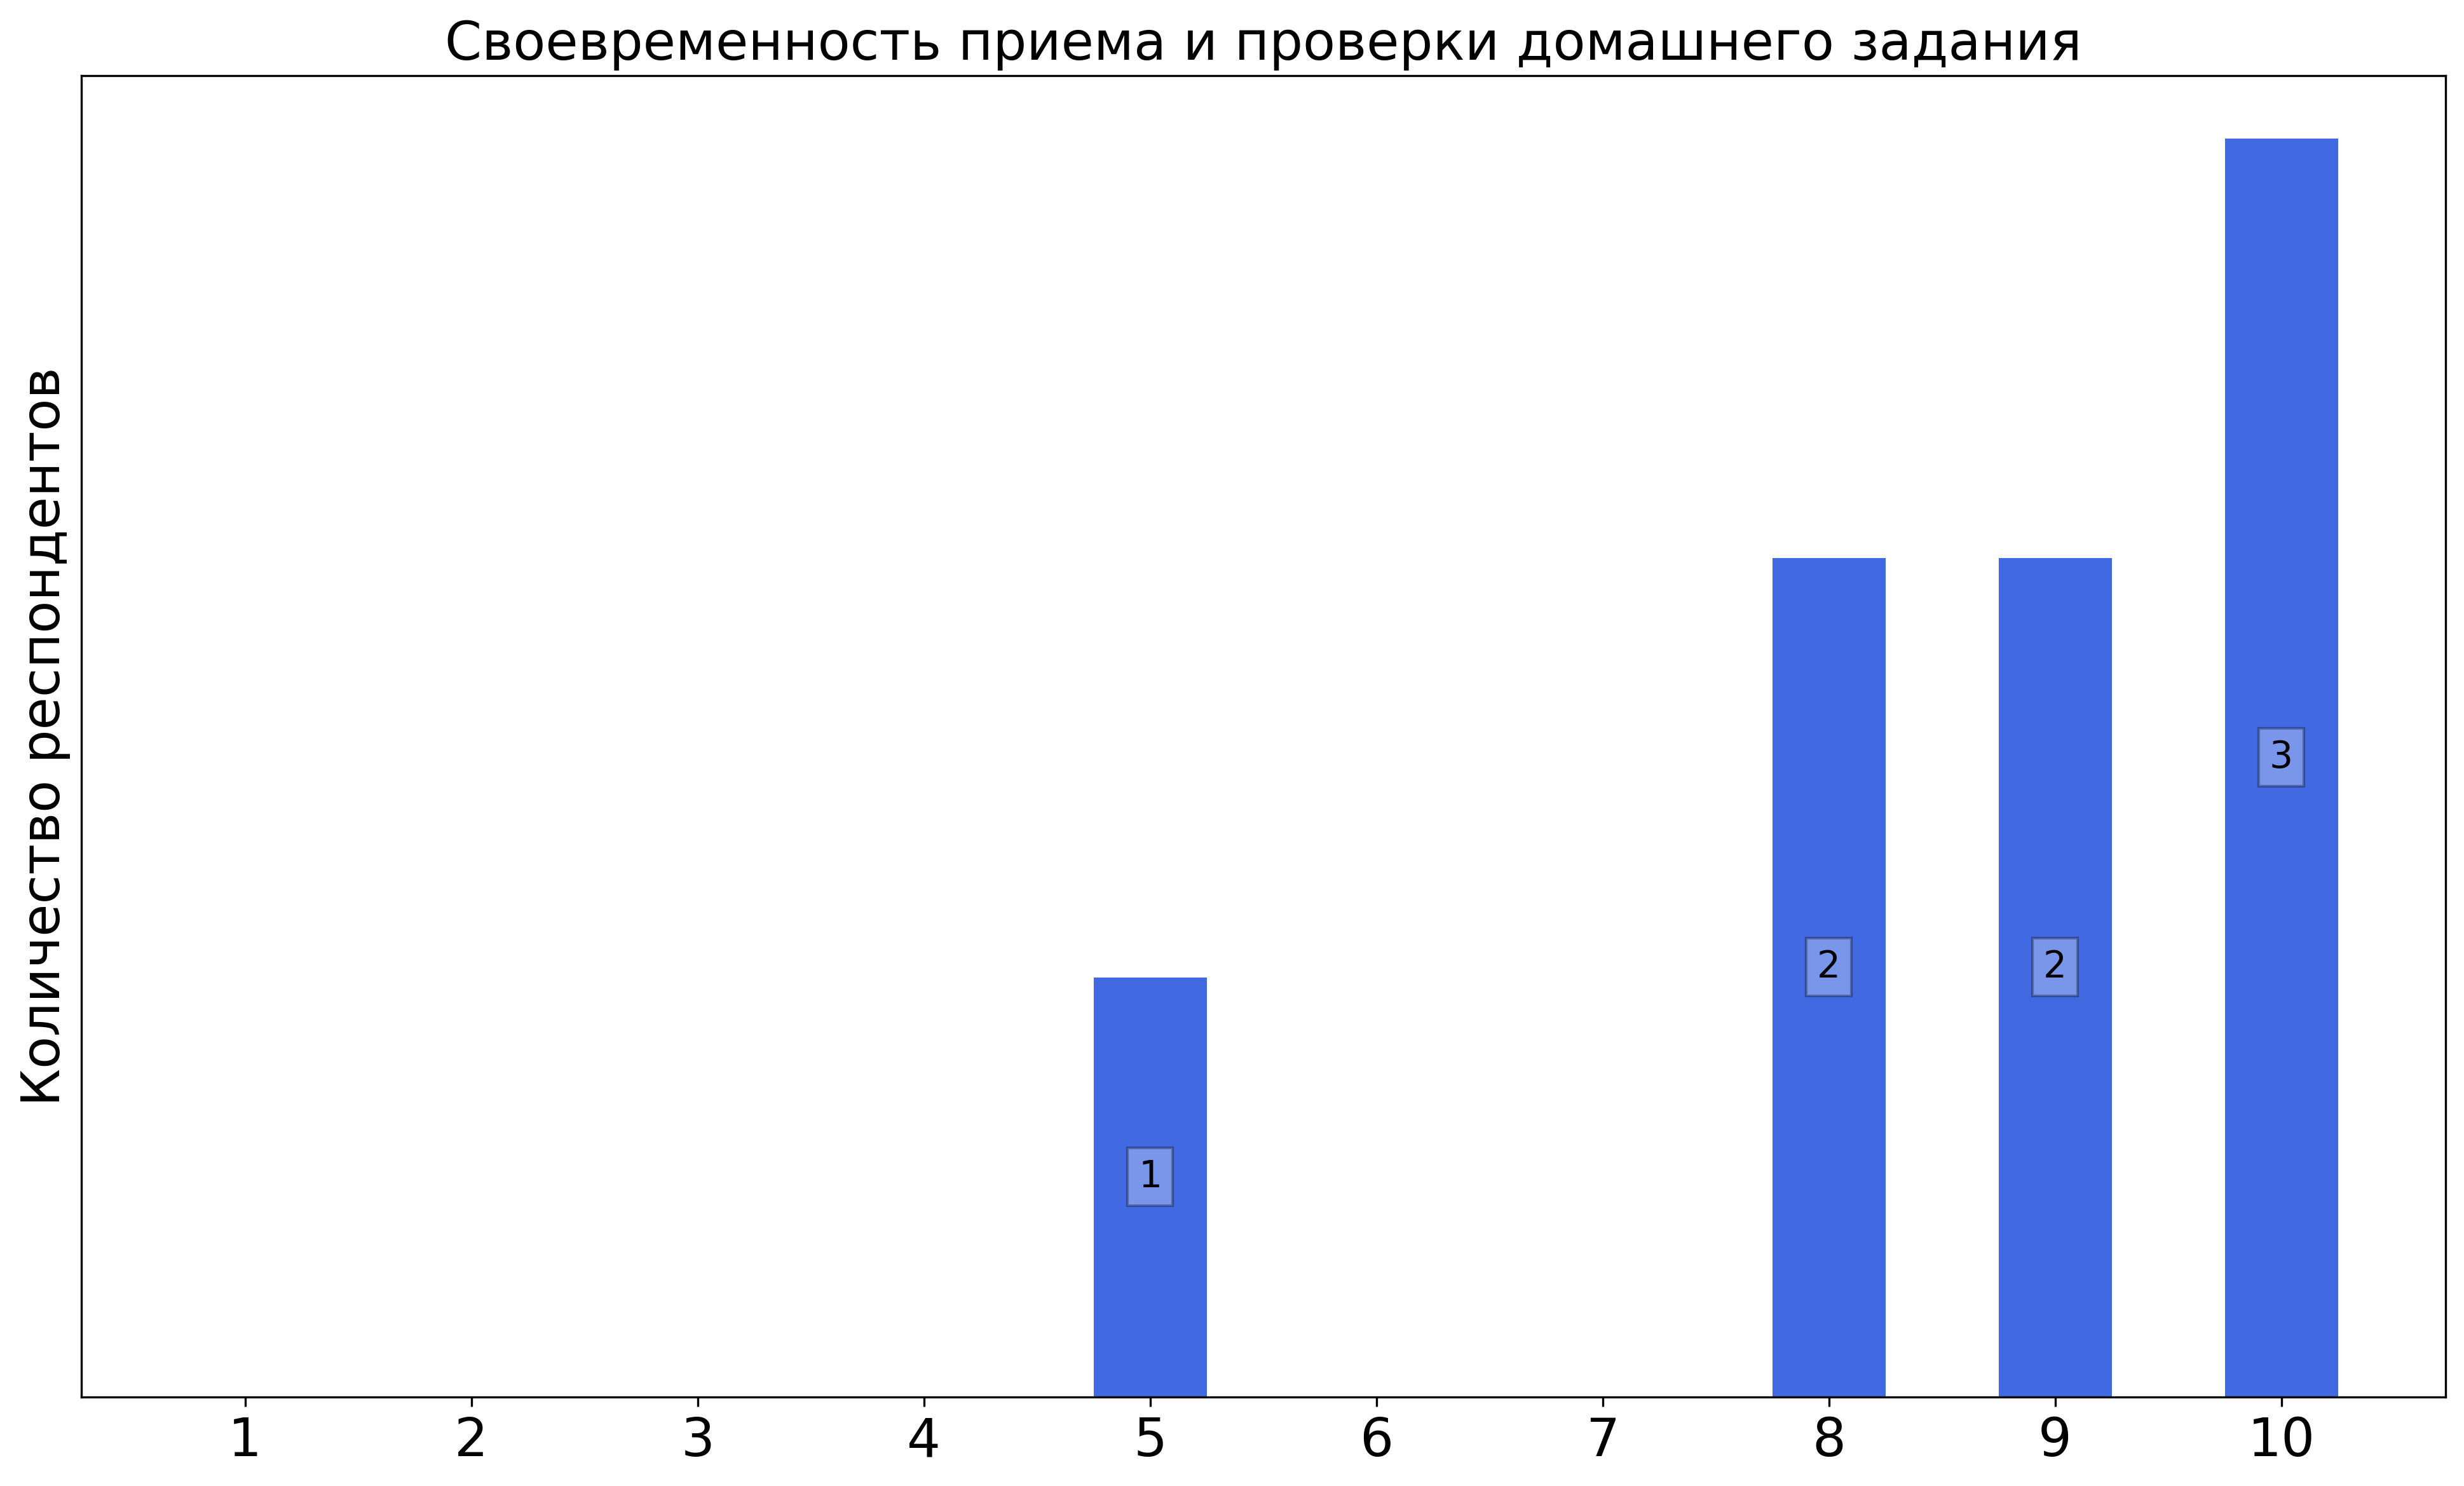
\includegraphics[width=\textwidth]{images/1 course/Общая физика - механика/seminarists-marks-Лилиенберг И.В.-2.png}
			\end{subfigure}
			\begin{subfigure}[b]{0.45\textwidth}
				\centering
				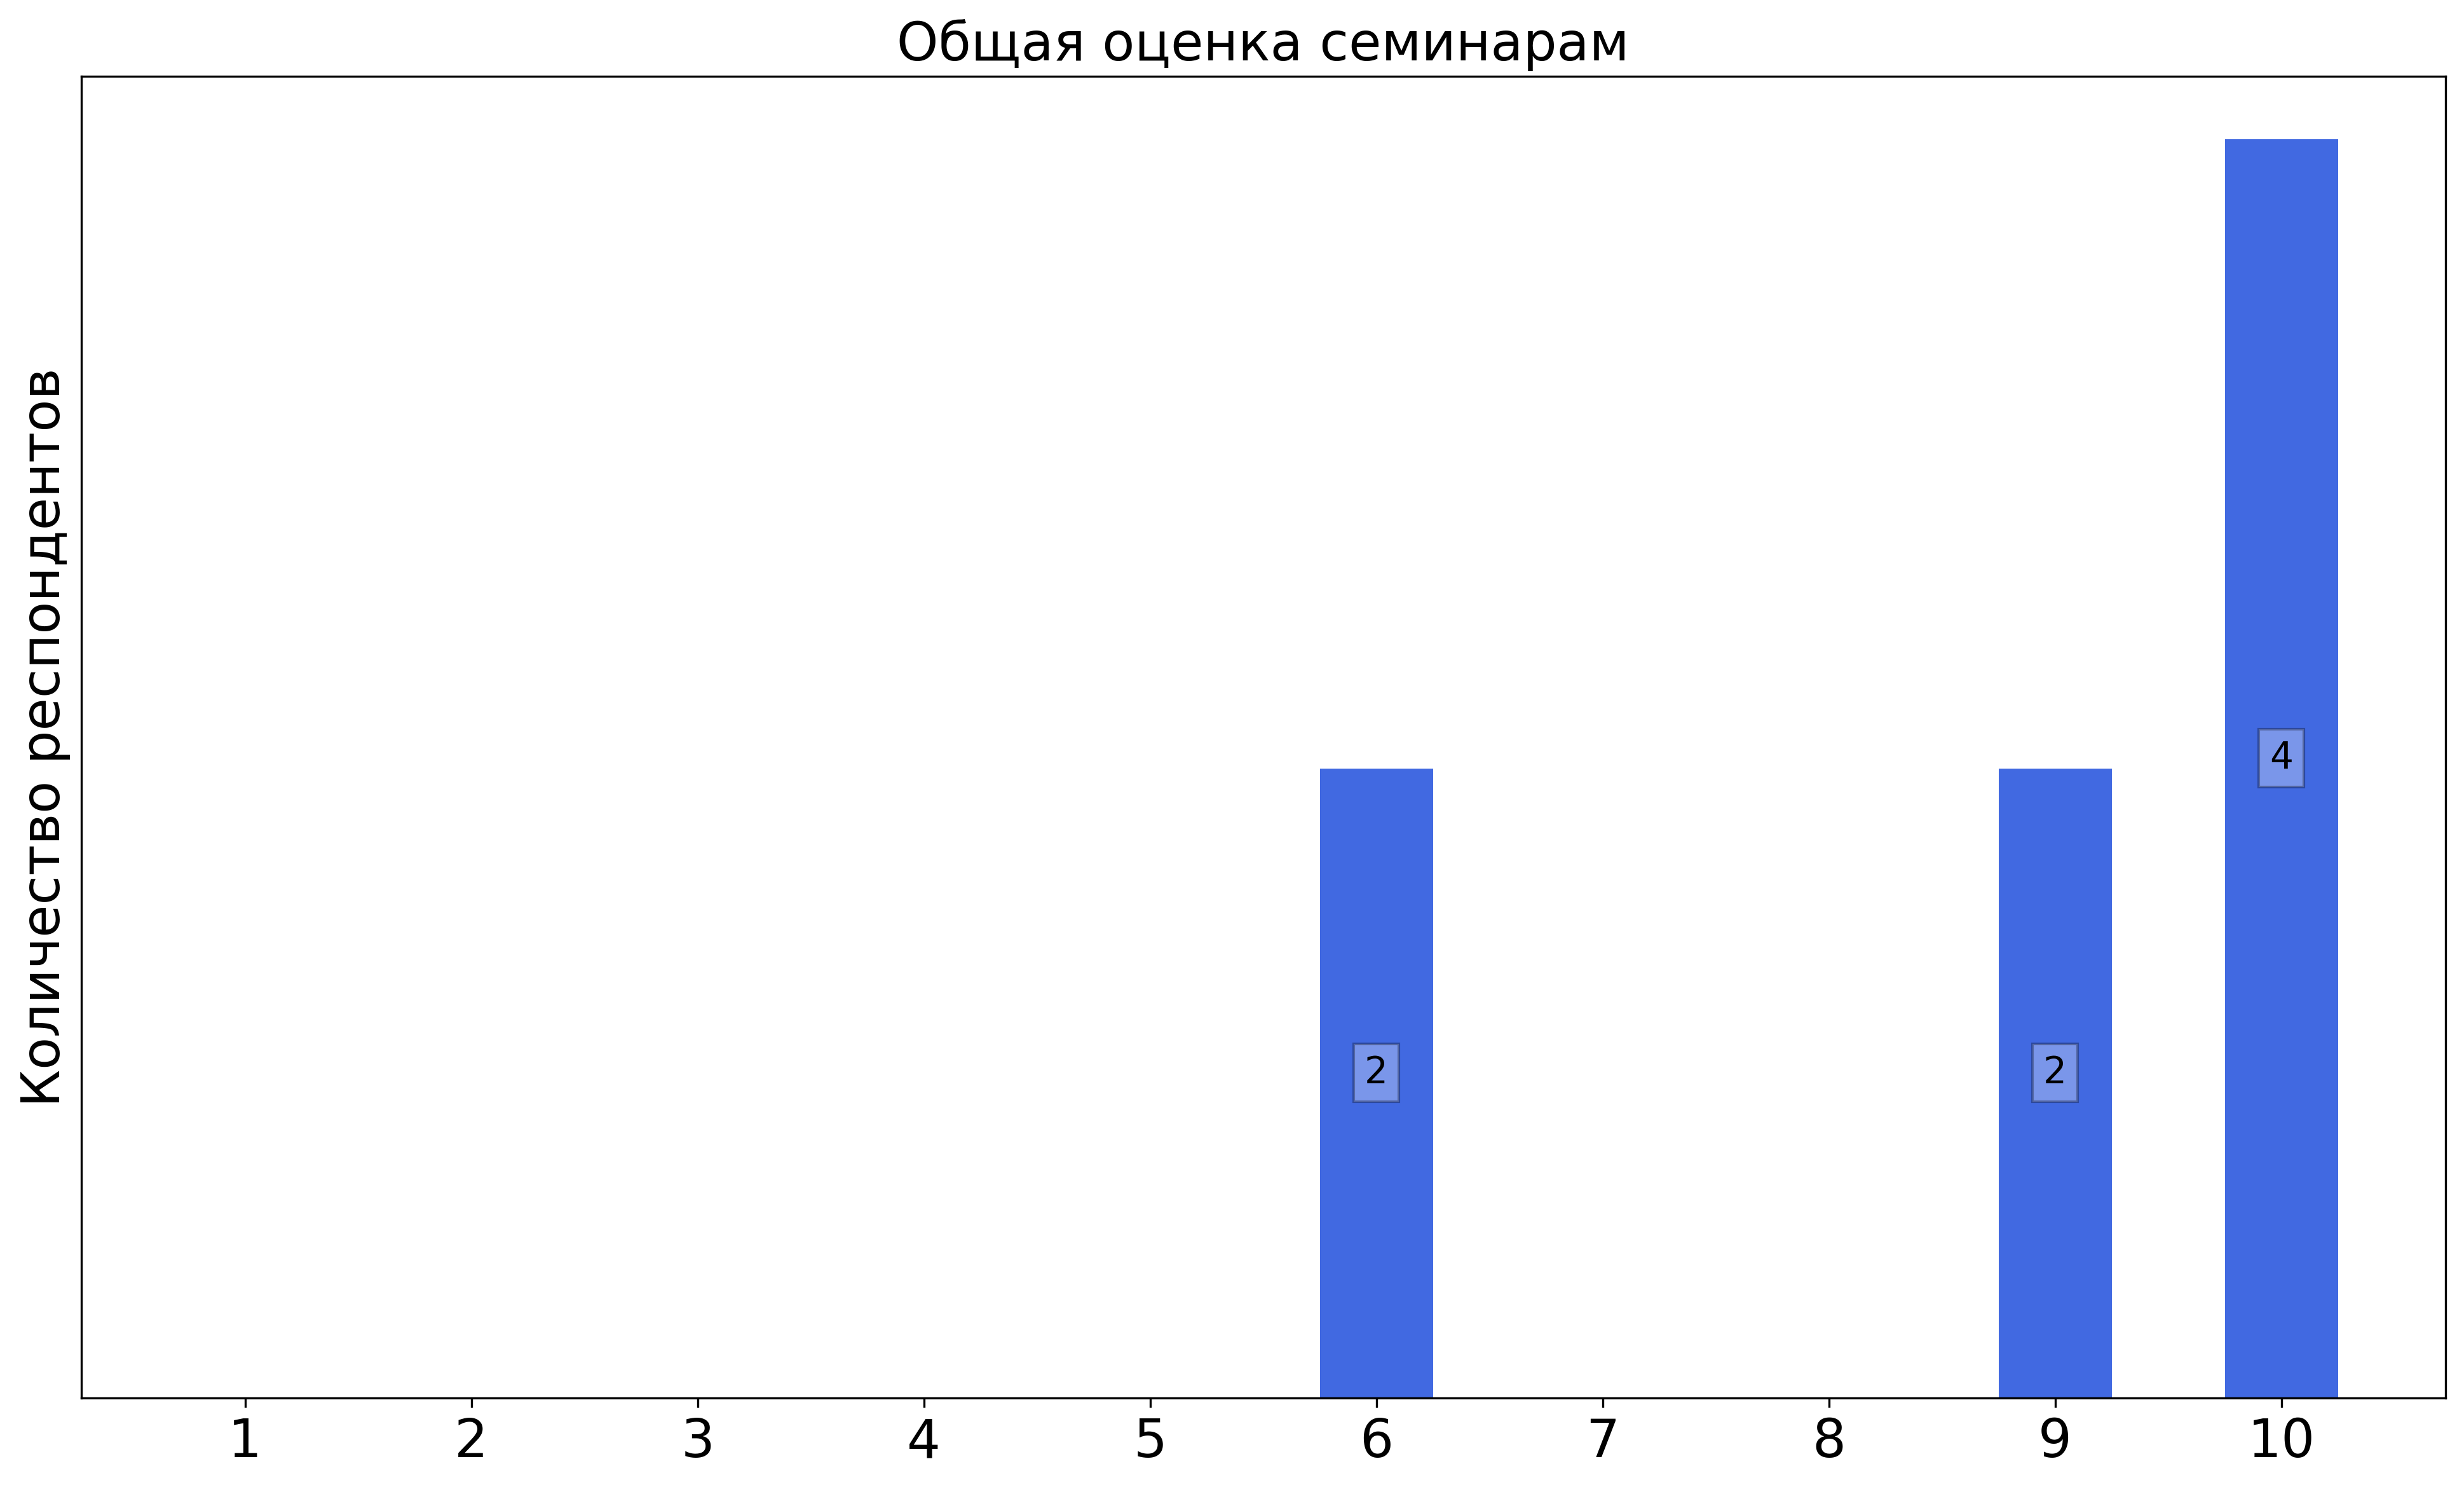
\includegraphics[width=\textwidth]{images/1 course/Общая физика - механика/seminarists-marks-Лилиенберг И.В.-3.png}
			\end{subfigure}	
			\caption{Оценки респондентов о качестве преподавания семинаров}
		\end{figure}

		\textbf{Комментарии студентов о семинаристе\protect\footnote{сохранены оригинальные орфография и пунктуация}}
            \begin{commentbox} 
                Всё здорово 
            \end{commentbox} 
        
            \begin{commentbox} 
                Хорошо объясняет теорию и сами задачи, успевает за семинар решить все еденички.  
            \end{commentbox} 
        
            \begin{commentbox} 
                На семинарах решает только семинарские задачи, ни больше ни меньше. Теорию рассказывает  плохо, буквально 2-3 формулы и дальше приступает к решению задач, а может вообще без теории начать. Сроки сдачи домашних работ у него плавущие. Сначала сказал, что можно ему в тг скидывать домашку, и он будет её засчитывать. Сначала всё было хорошо, он действительно смотрел дз и задавал вопросы по нему. Но спустя где-то месяца полтора он просто стал игнорировать, то есть он читает вопросы, но сам ничего не отвечает. Или отвечал спустя три недели. Пришлось лично идти и сдавать домашнее задание 
            \end{commentbox} 
					
	\subsubsection{Отзыв студентов о семинарах. Семинарист: Стожков В.Ю.}
		\begin{figure}[H]
			\centering
			\begin{subfigure}[b]{0.45\textwidth}
				\centering
				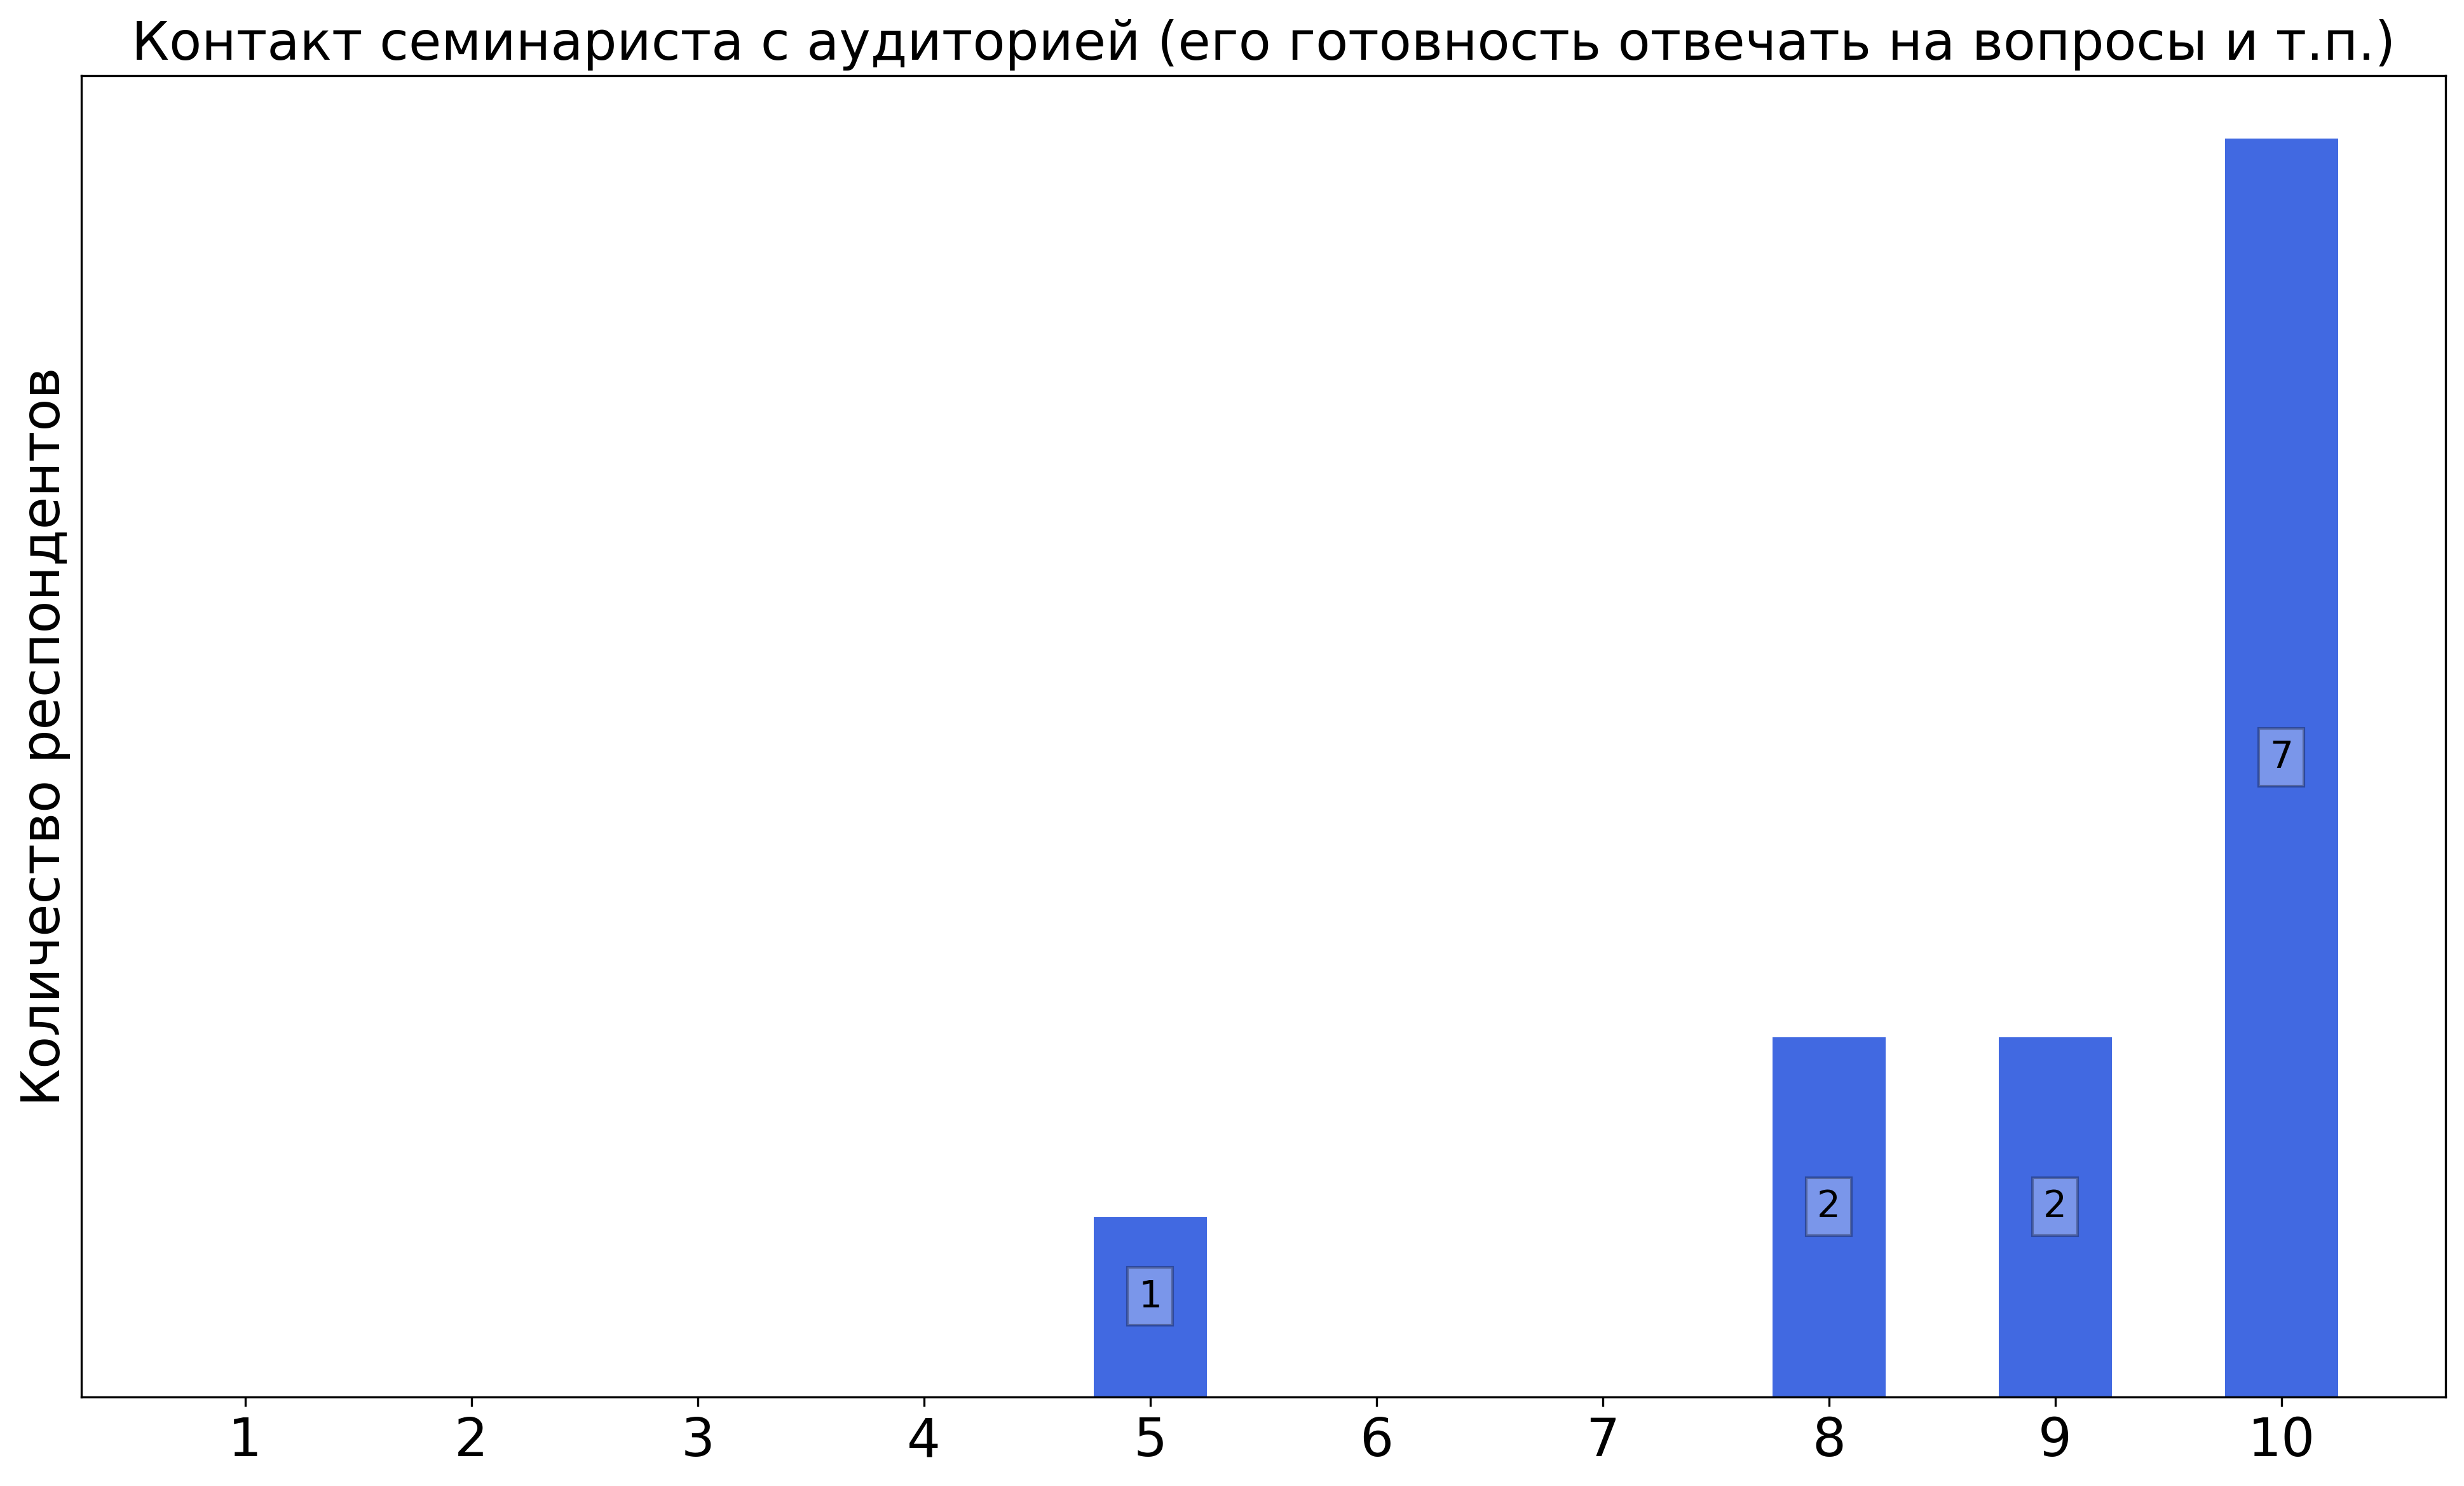
\includegraphics[width=\textwidth]{images/1 course/Общая физика - механика/seminarists-marks-Стожков В.Ю.-0.png}
			\end{subfigure}
			\begin{subfigure}[b]{0.45\textwidth}
				\centering
				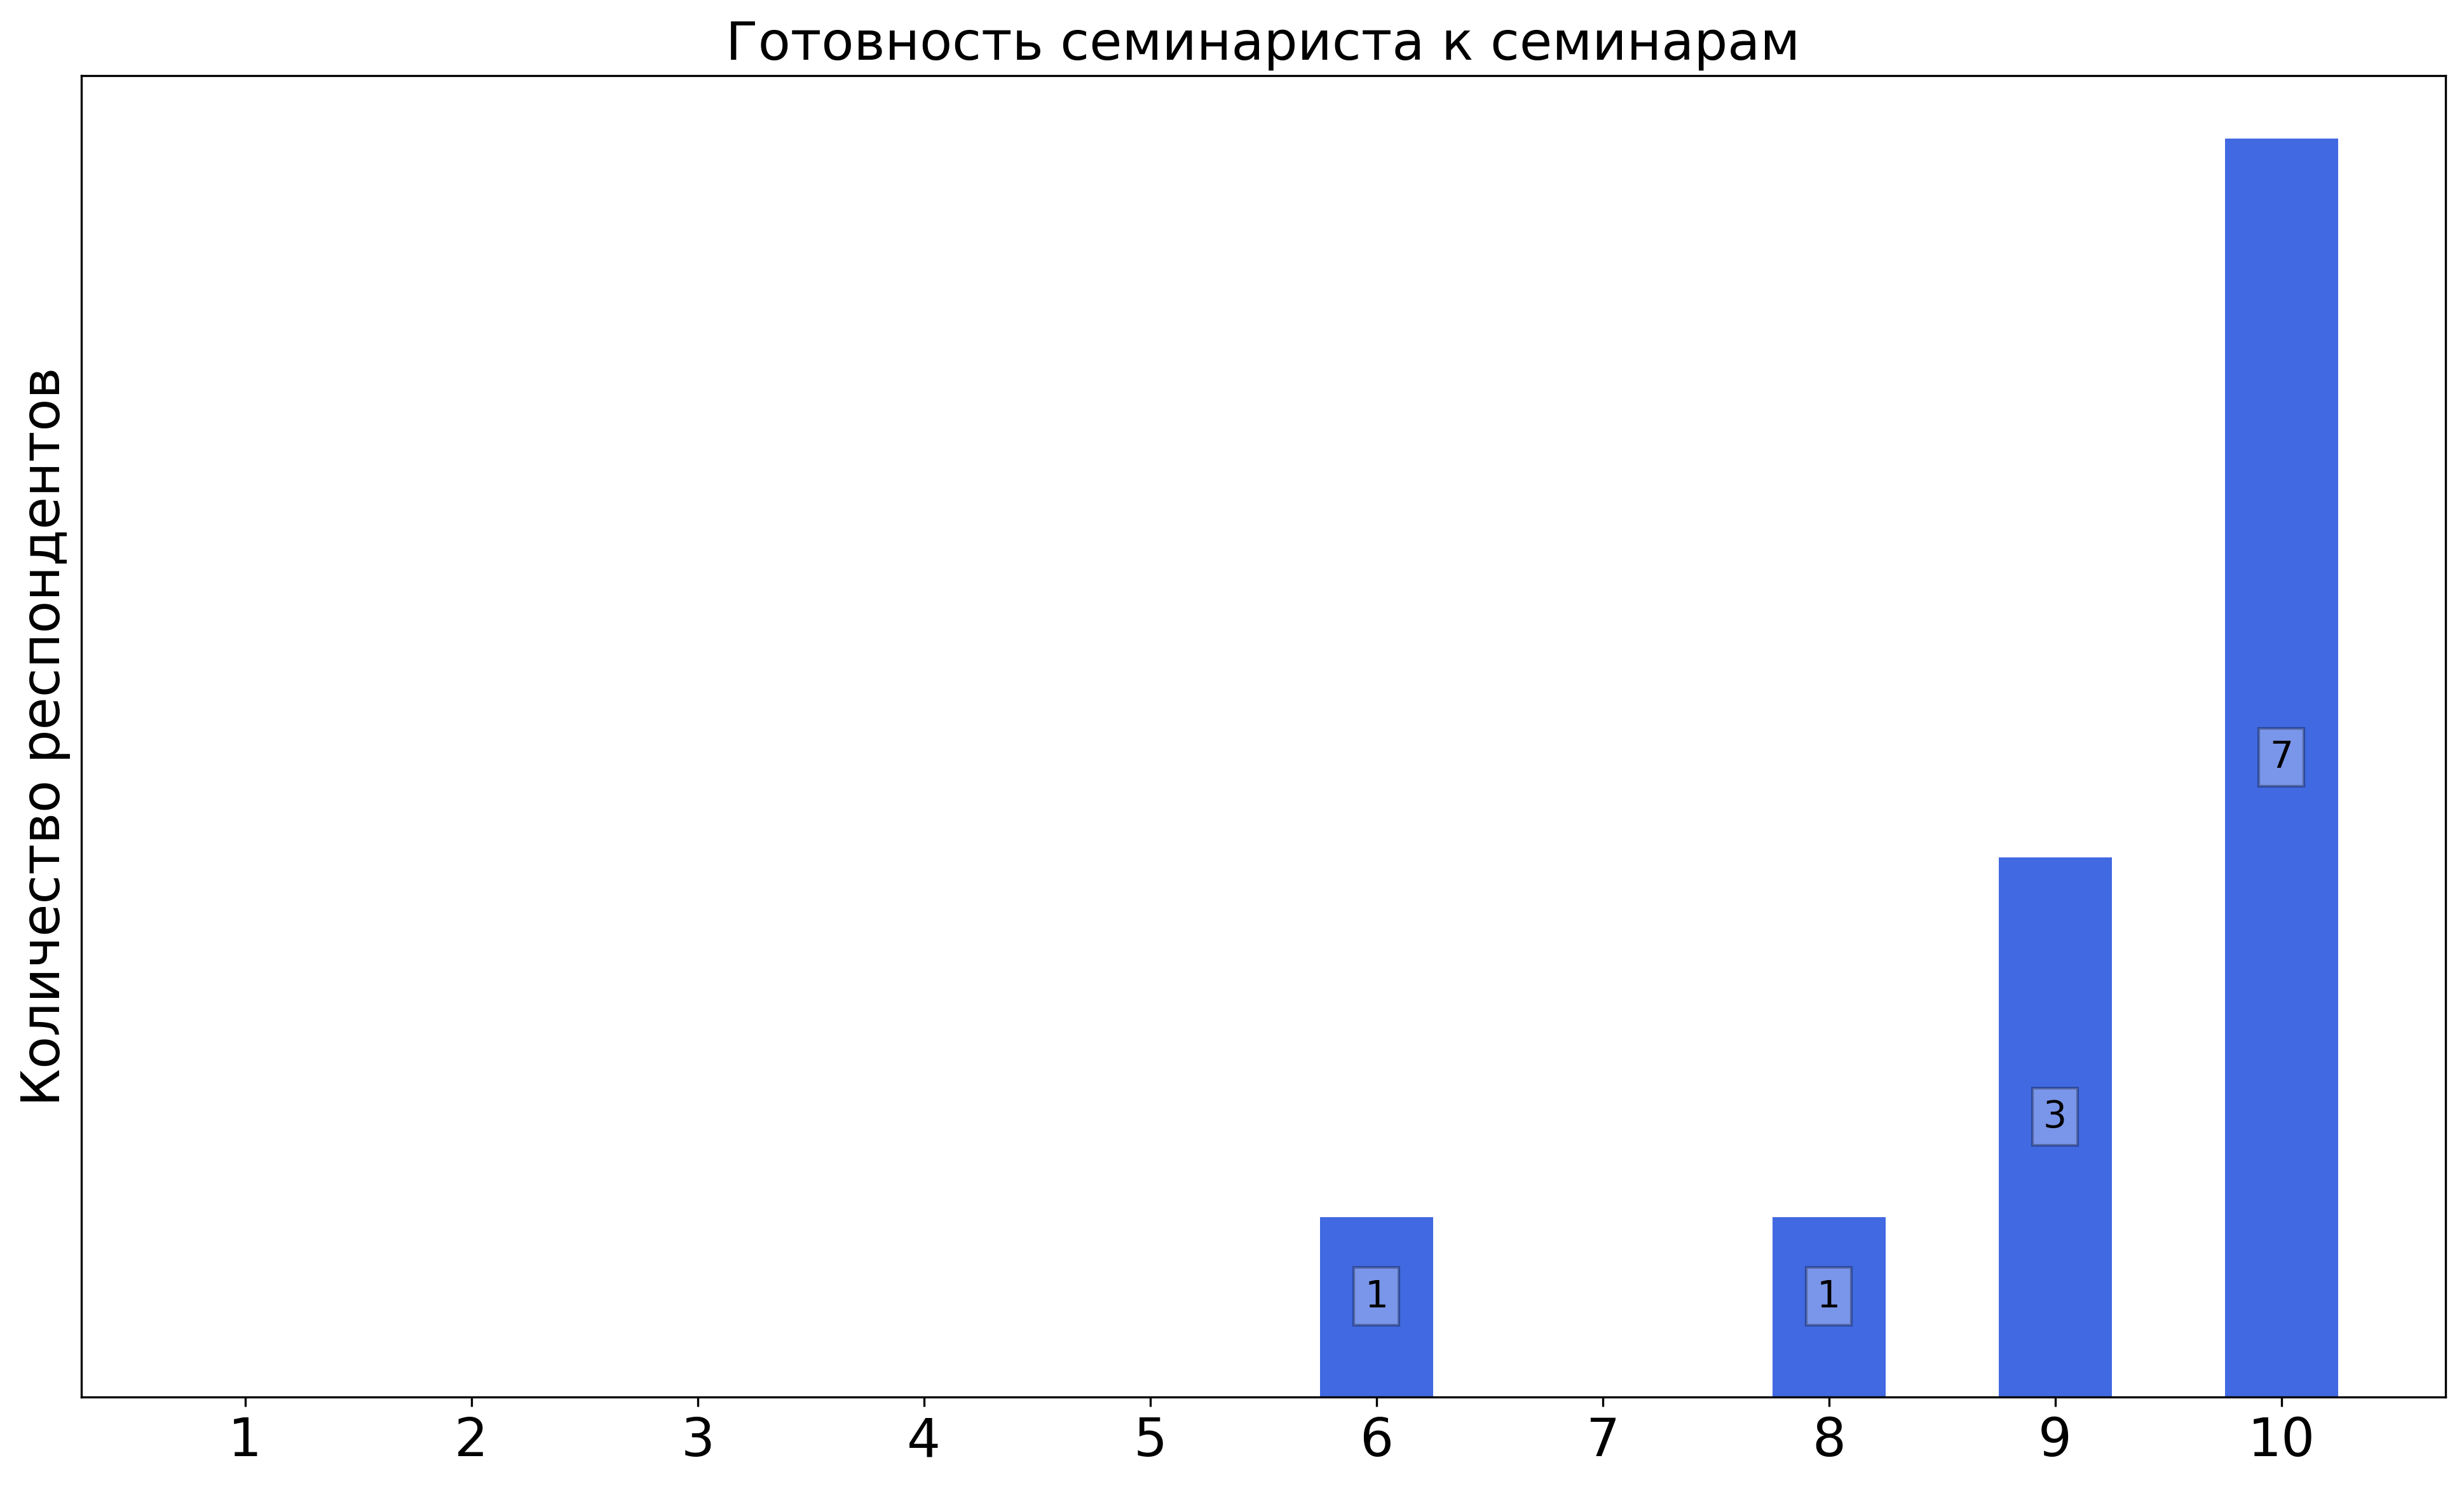
\includegraphics[width=\textwidth]{images/1 course/Общая физика - механика/seminarists-marks-Стожков В.Ю.-1.png}
			\end{subfigure}
			\begin{subfigure}[b]{0.45\textwidth}
				\centering
				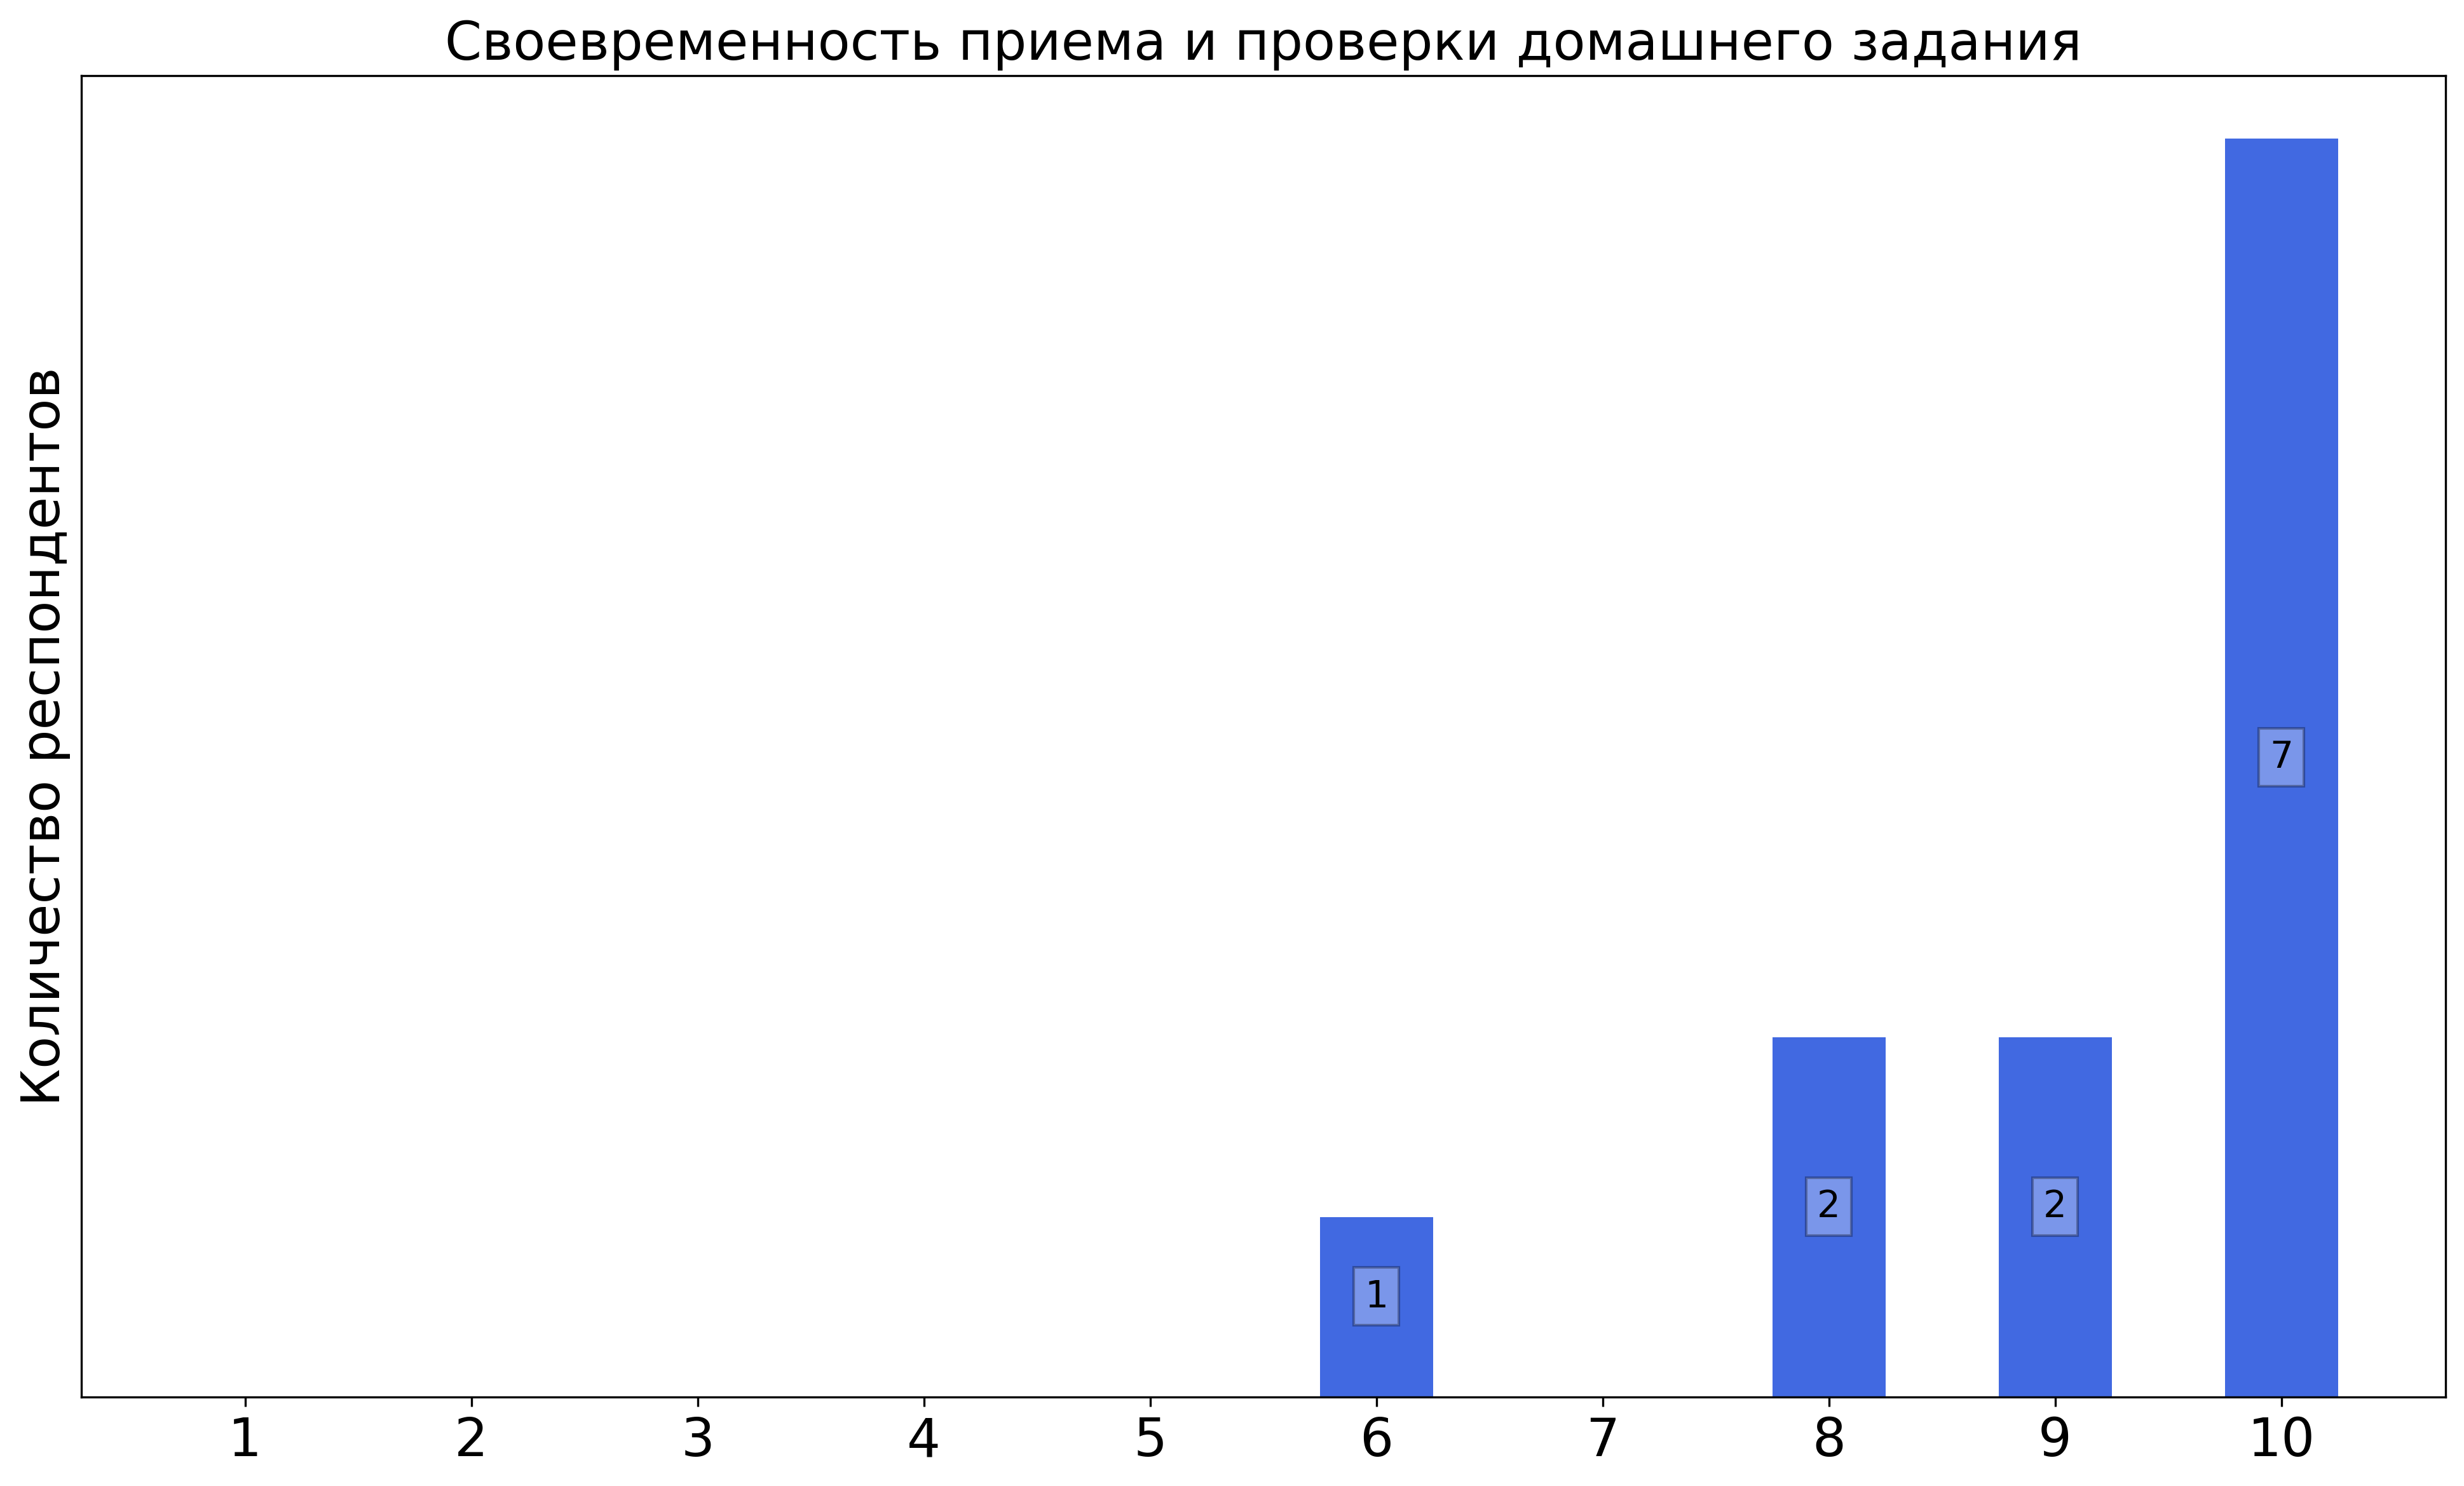
\includegraphics[width=\textwidth]{images/1 course/Общая физика - механика/seminarists-marks-Стожков В.Ю.-2.png}
			\end{subfigure}
			\begin{subfigure}[b]{0.45\textwidth}
				\centering
				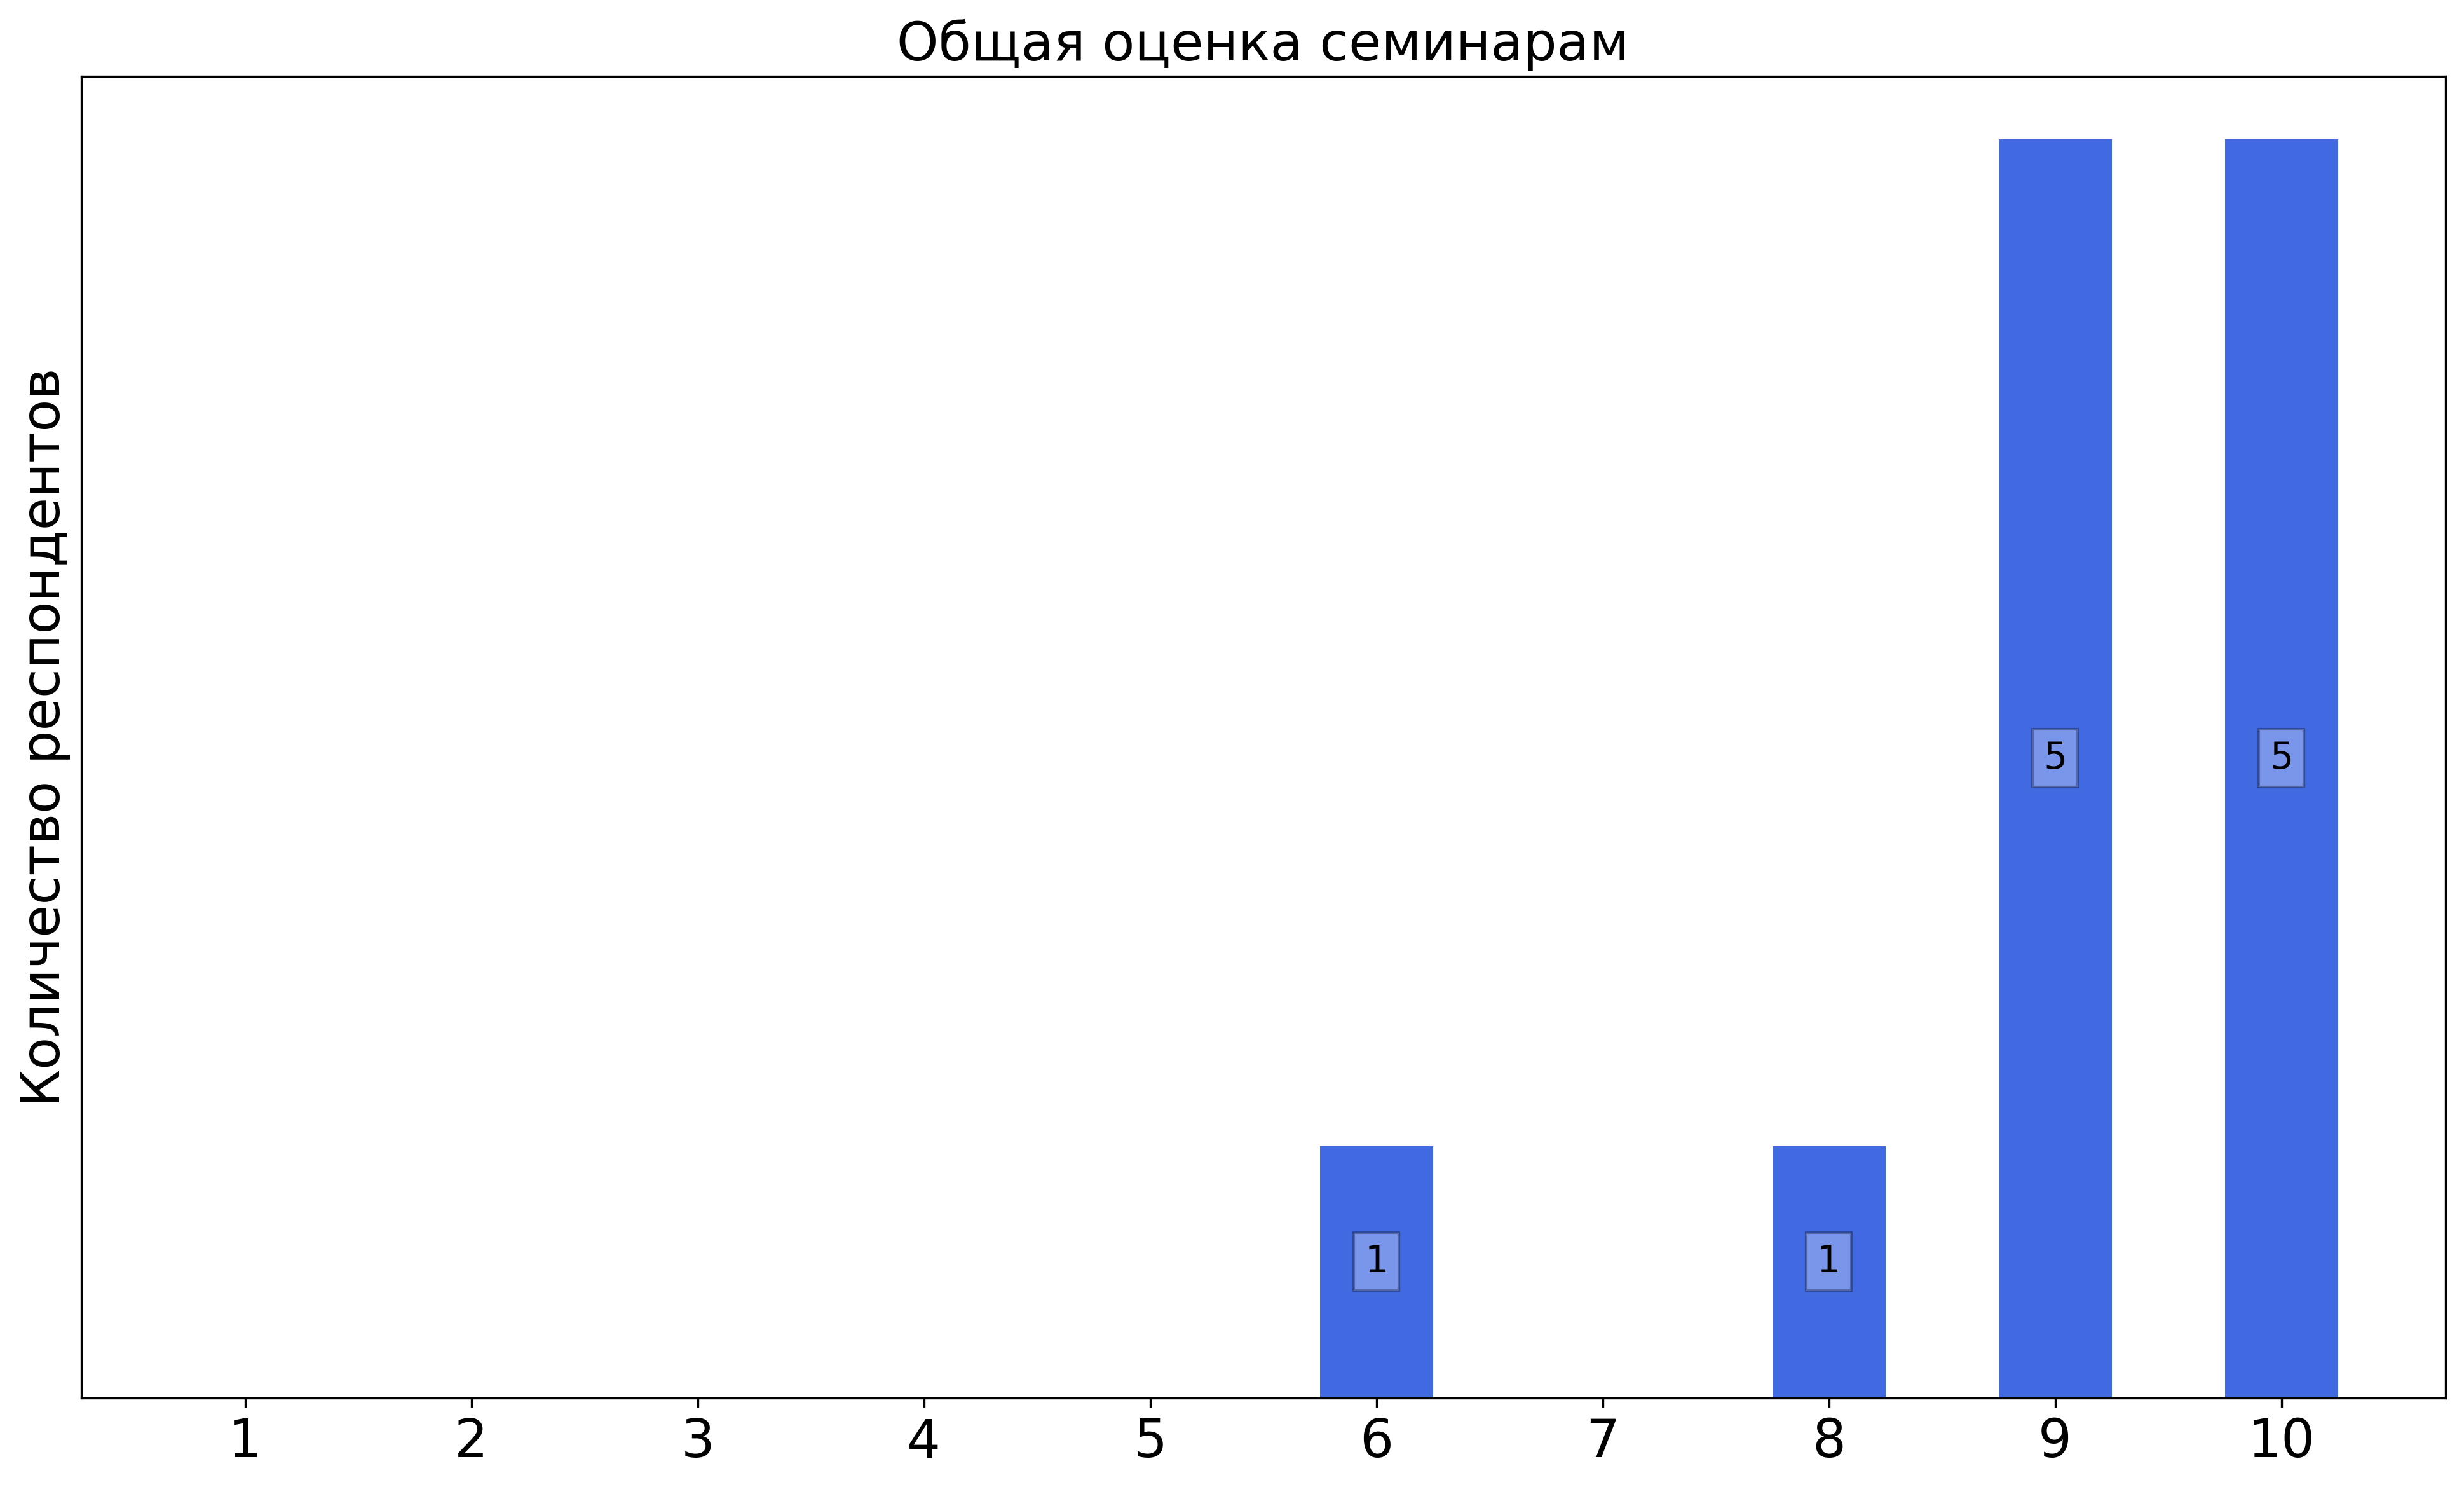
\includegraphics[width=\textwidth]{images/1 course/Общая физика - механика/seminarists-marks-Стожков В.Ю.-3.png}
			\end{subfigure}	
			\caption{Оценки респондентов о качестве преподавания семинаров}
		\end{figure}

		\textbf{Комментарии студентов о семинаристе\protect\footnote{сохранены оригинальные орфография и пунктуация}}
            \begin{commentbox} 
                мужик ровный  
            \end{commentbox} 
        
            \begin{commentbox} 
                Семинары у Стожкова В.Ю. довольно медленные, но интересные и "сильно концентрированные" обсуждениями физической сути задач 
            \end{commentbox} 


	\subsubsection{Отзыв студентов о семинарах. Семинарист: Удалова А.Г.}
		\begin{figure}[H]
			\centering
			\begin{subfigure}[b]{0.45\textwidth}
				\centering
				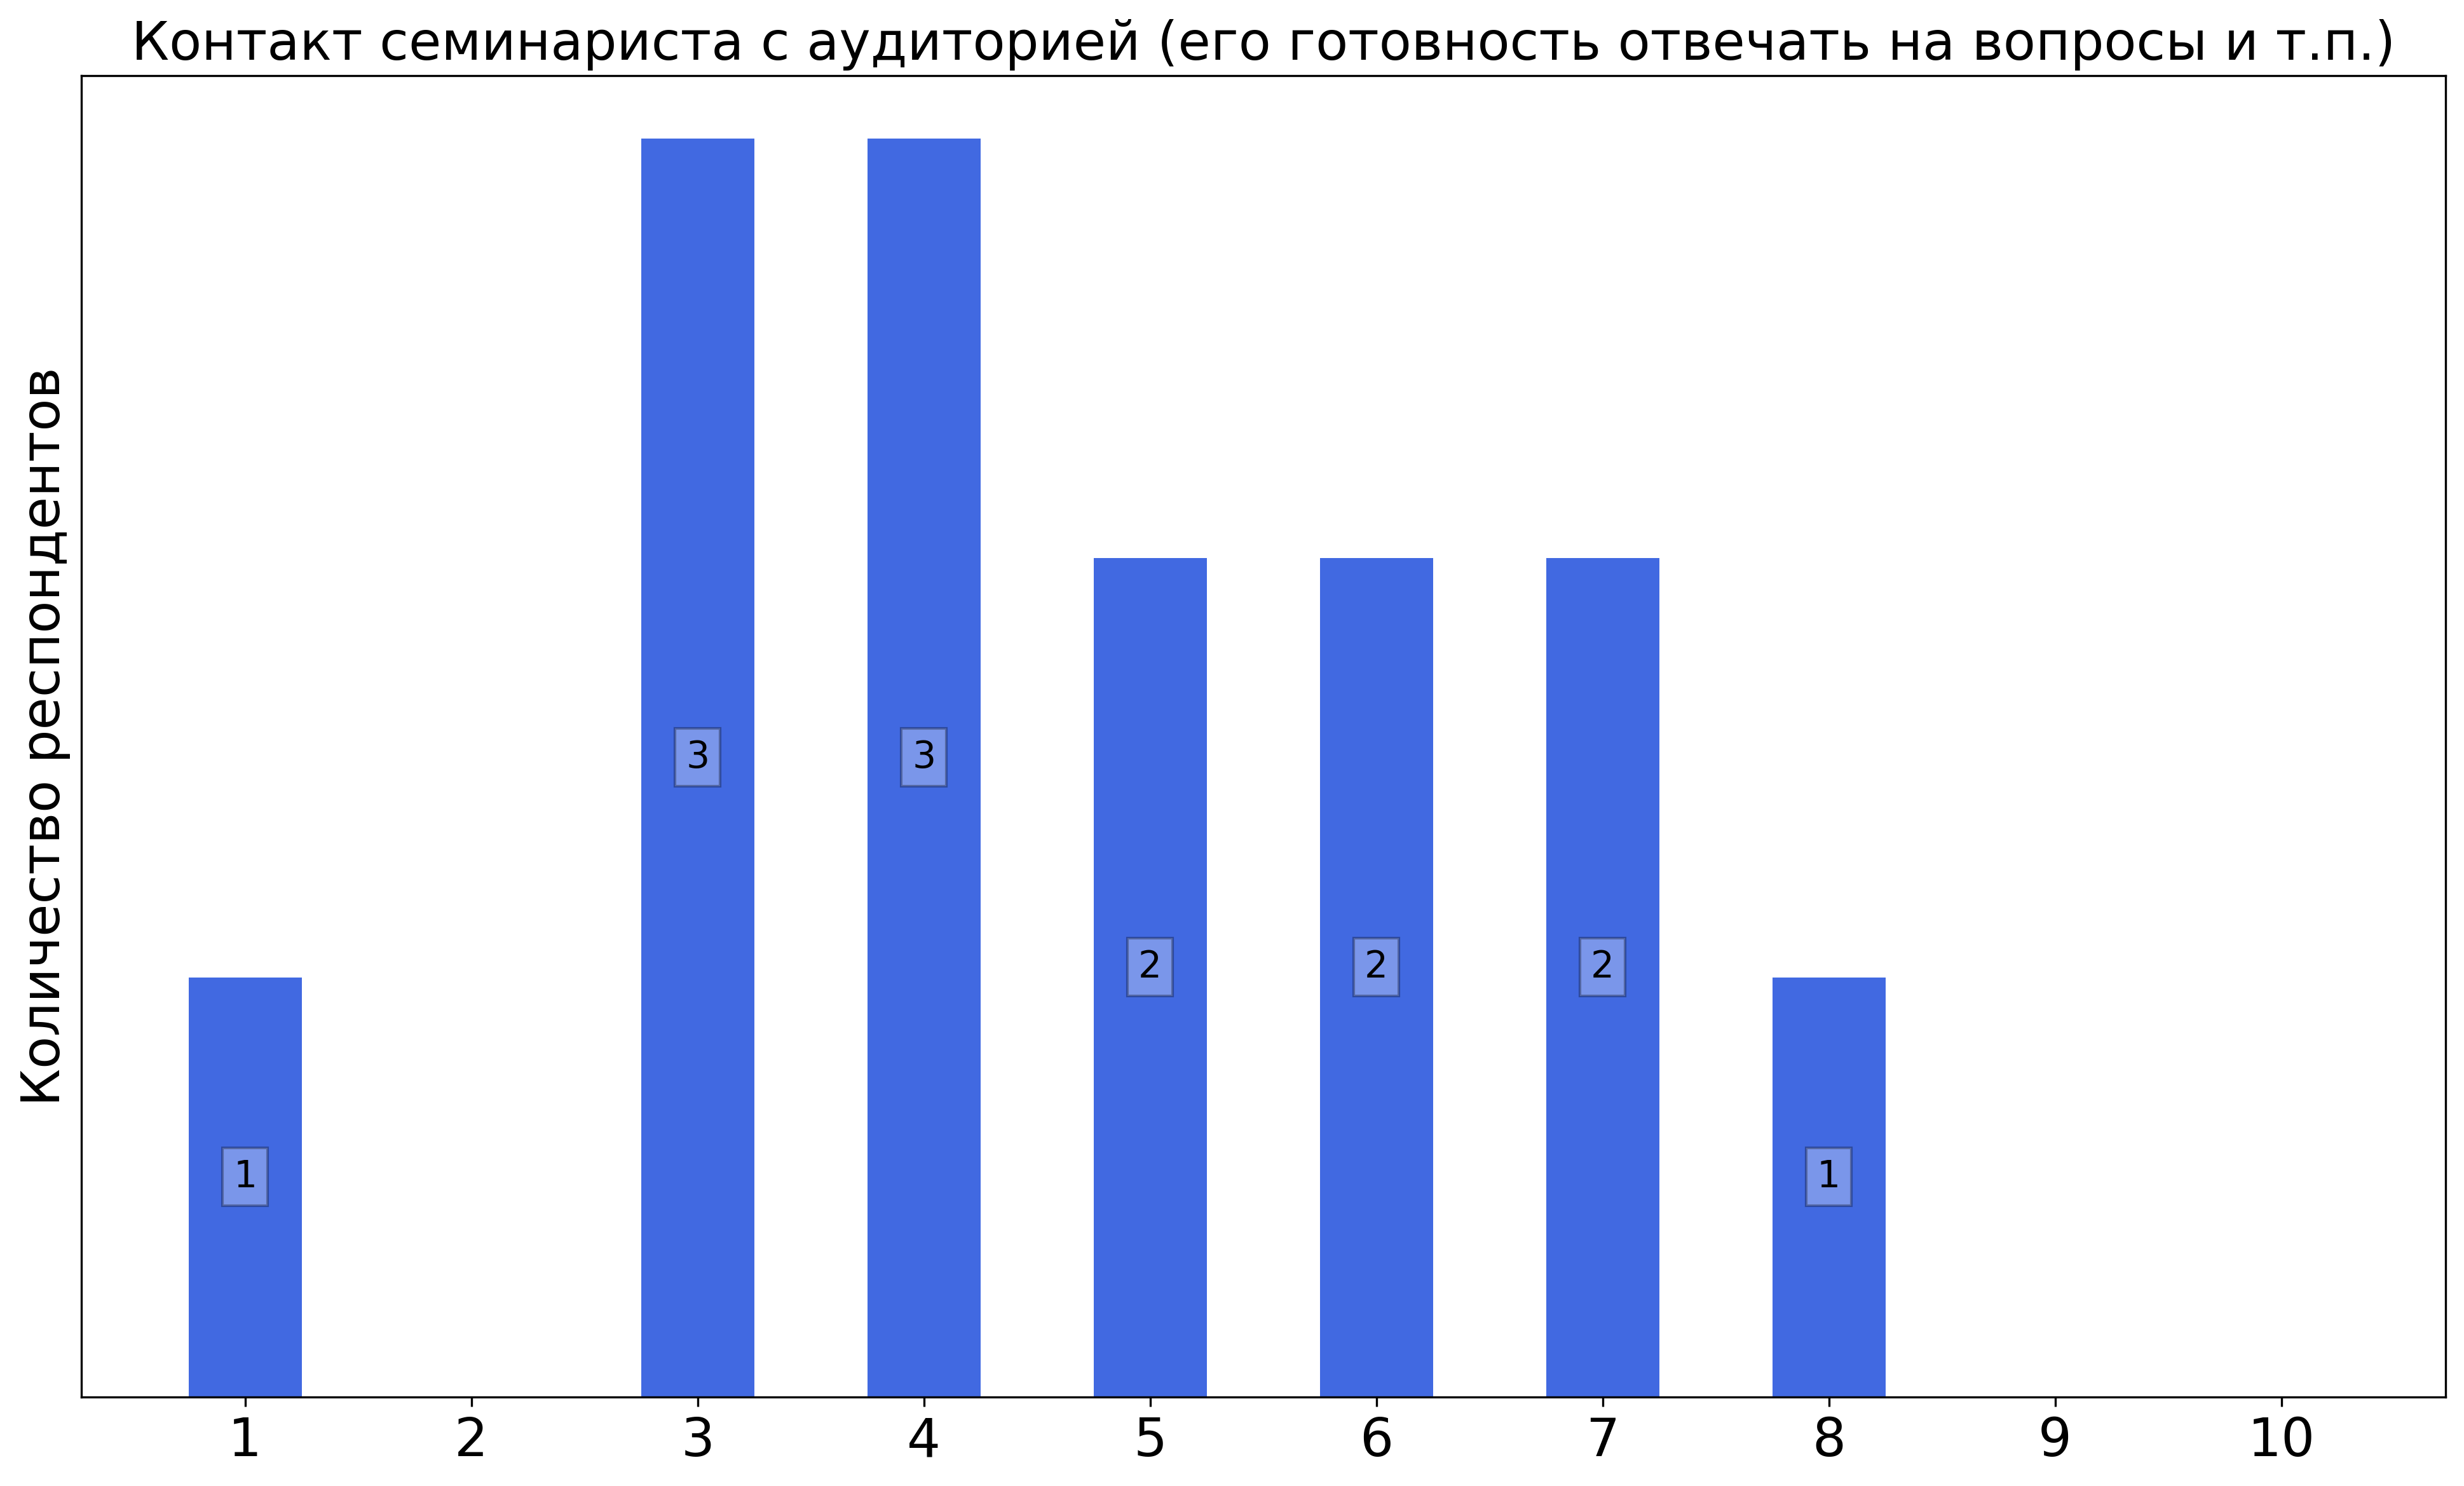
\includegraphics[width=\textwidth]{images/1 course/Общая физика - механика/seminarists-marks-Удалова А.Г.-0.png}
			\end{subfigure}
			\begin{subfigure}[b]{0.45\textwidth}
				\centering
				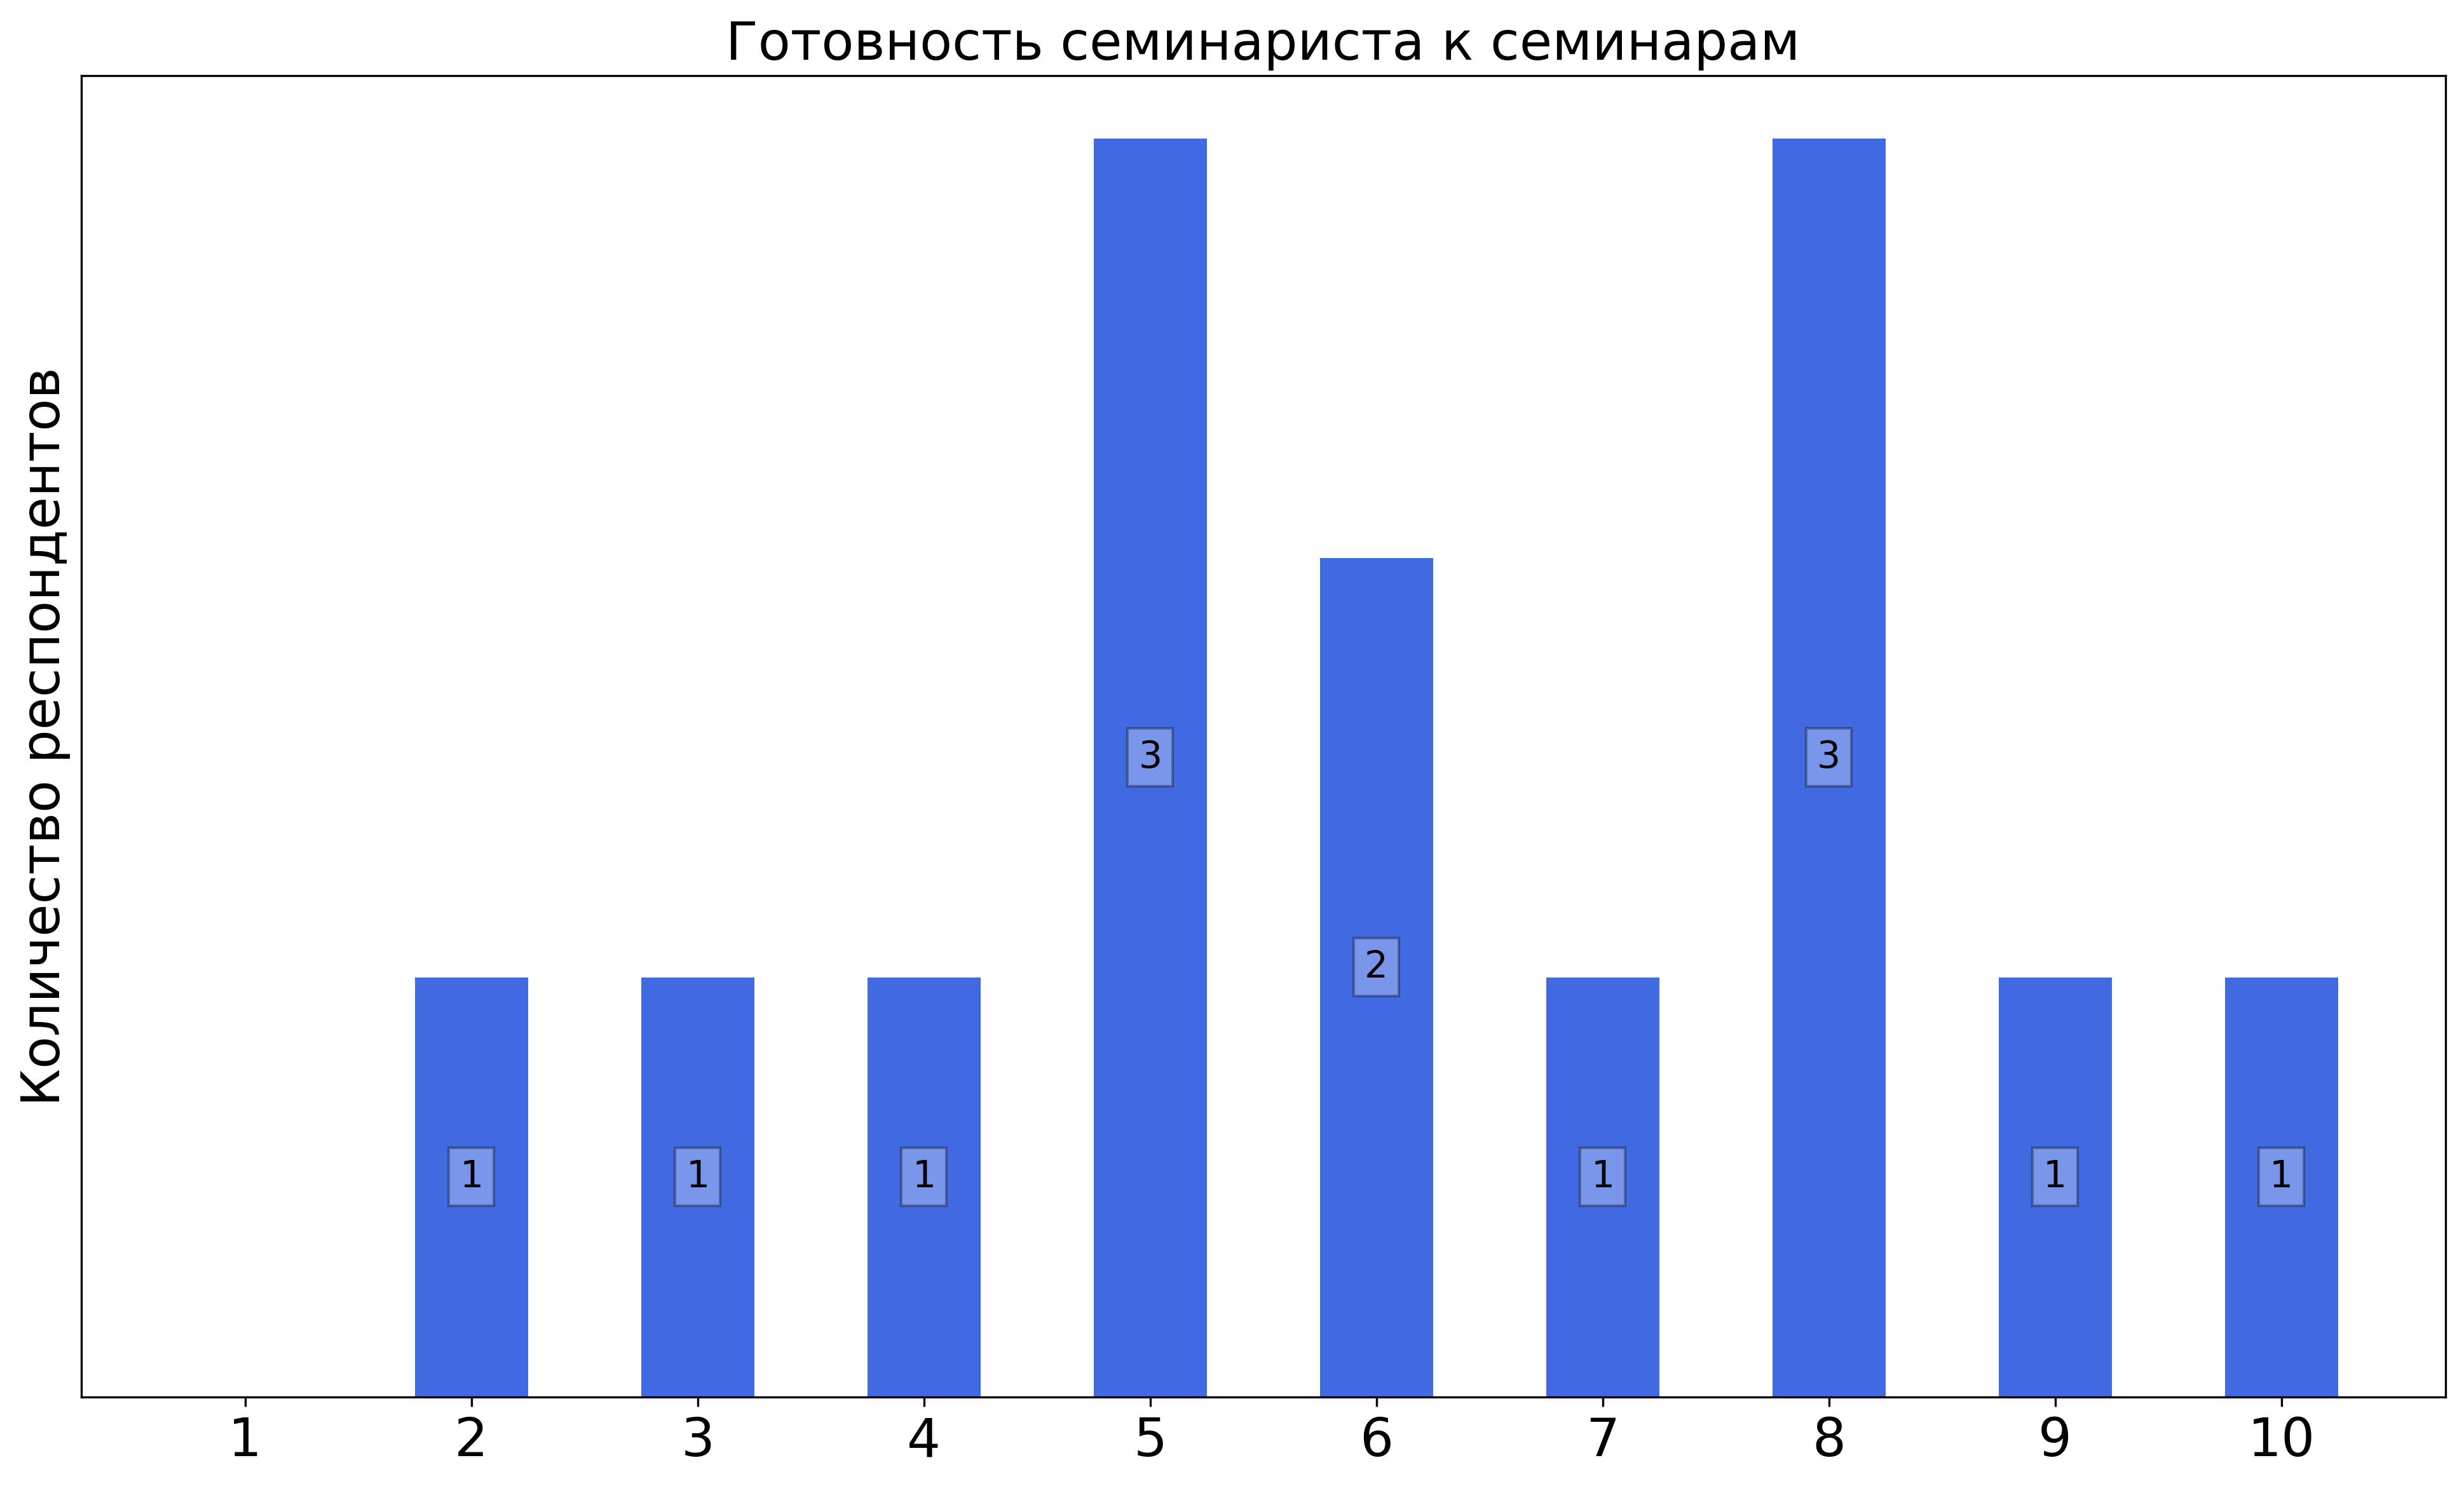
\includegraphics[width=\textwidth]{images/1 course/Общая физика - механика/seminarists-marks-Удалова А.Г.-1.png}
			\end{subfigure}
			\begin{subfigure}[b]{0.45\textwidth}
				\centering
				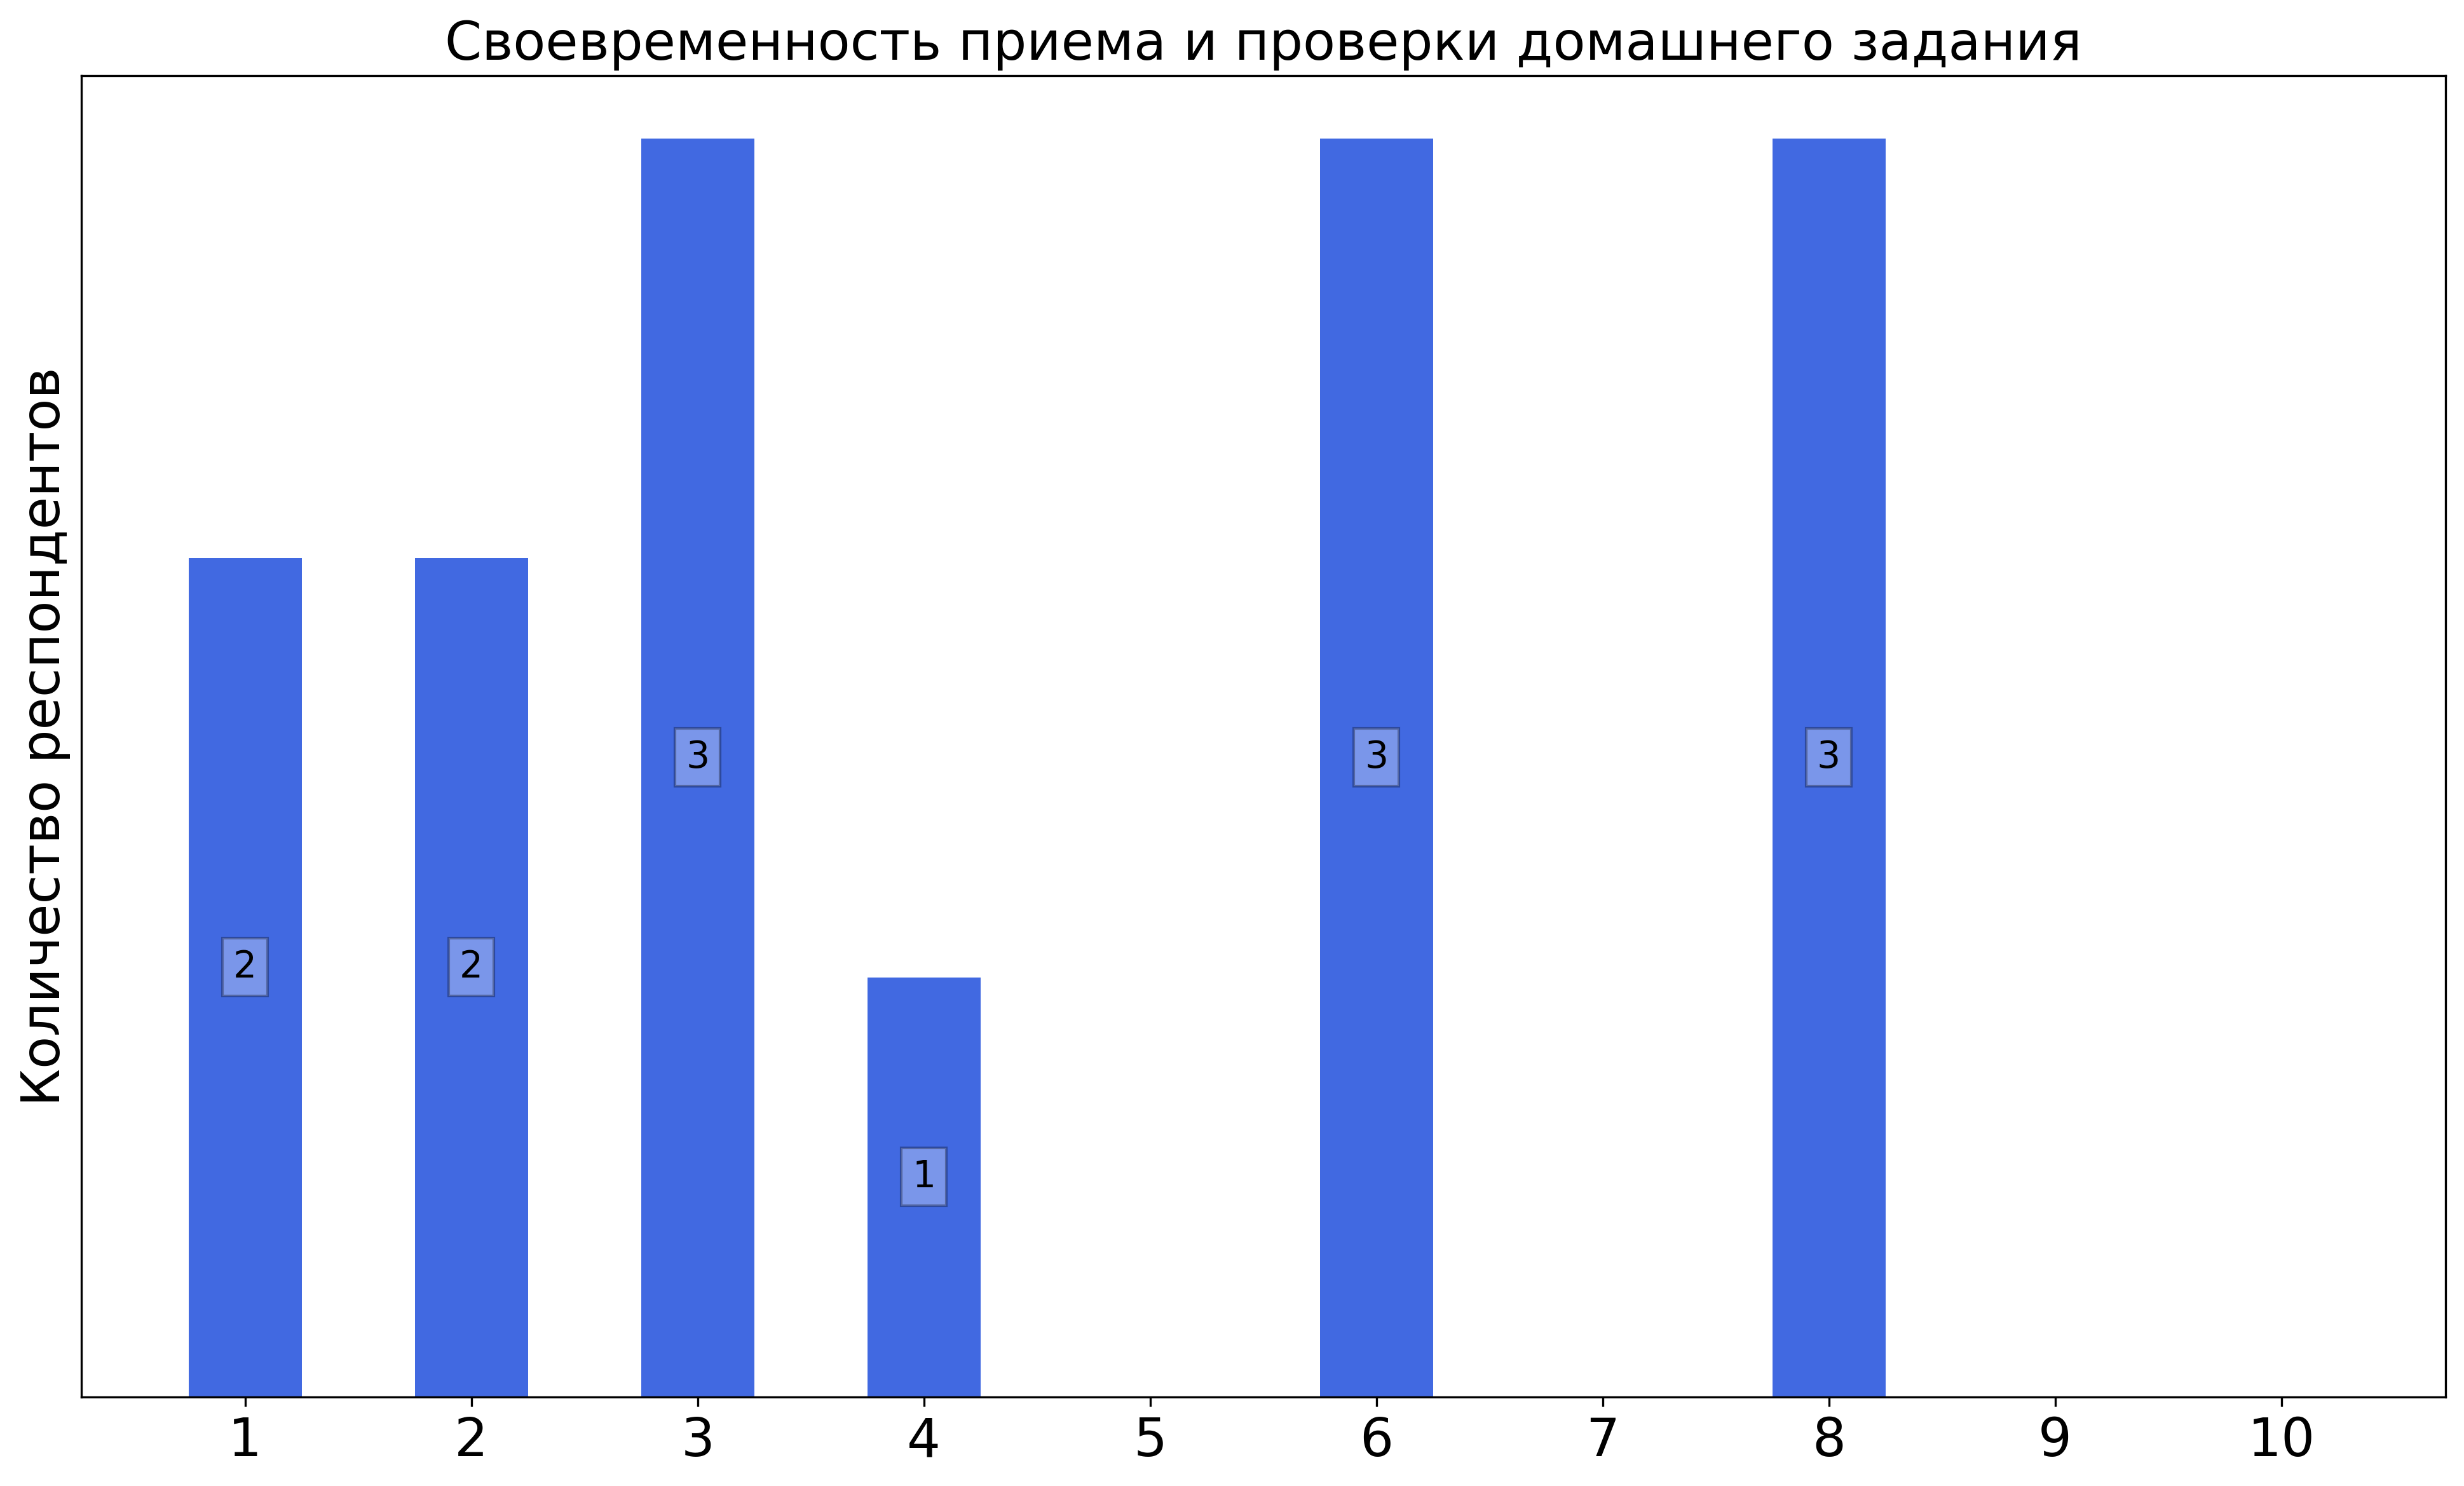
\includegraphics[width=\textwidth]{images/1 course/Общая физика - механика/seminarists-marks-Удалова А.Г.-2.png}
			\end{subfigure}
			\begin{subfigure}[b]{0.45\textwidth}
				\centering
				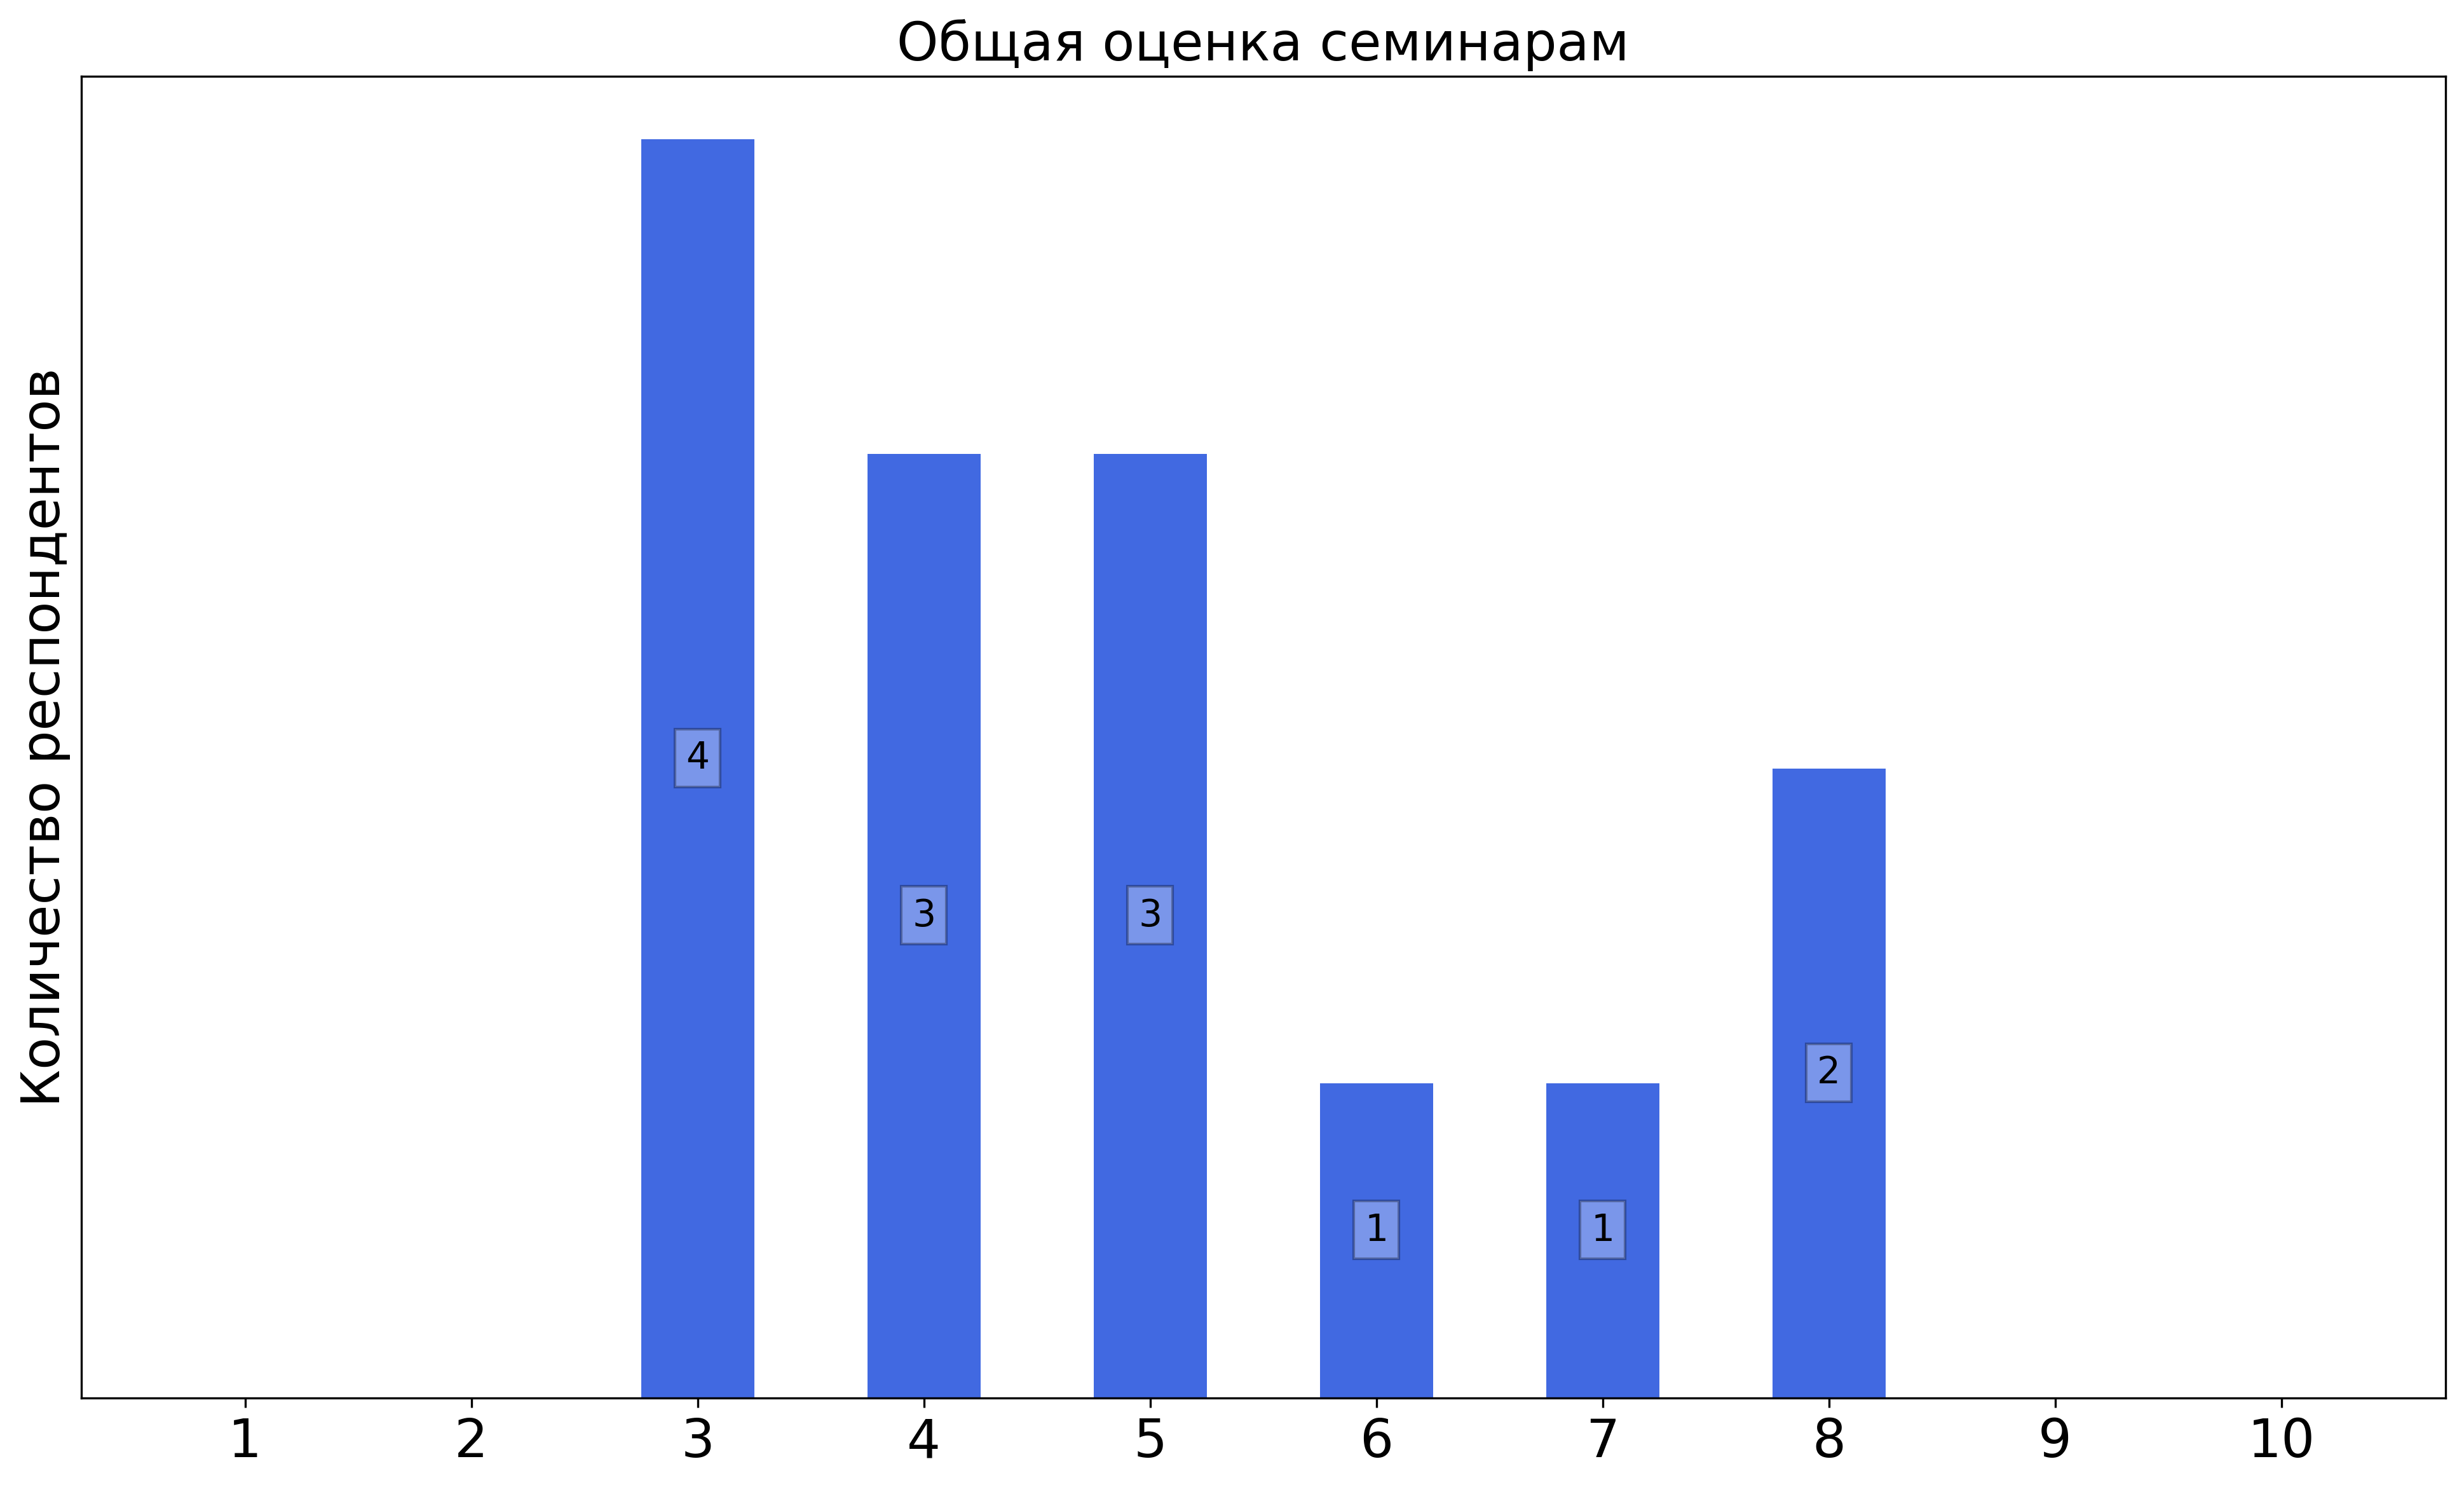
\includegraphics[width=\textwidth]{images/1 course/Общая физика - механика/seminarists-marks-Удалова А.Г.-3.png}
			\end{subfigure}	
			\caption{Оценки респондентов о качестве преподавания семинаров}
		\end{figure}

		\textbf{Комментарии студентов о семинаристе\protect\footnote{сохранены оригинальные орфография и пунктуация}}
            \begin{commentbox} 
                Первые пару недель было впечатление, что я знаю физику лучше, чем преподаватель. Предмет знает плохо, объясняет непонятно, на вопрос "почему" может запросто ответить что-то в духе "формула такая". ДЗ и контрольные оценивает лояльно, но с большим опозданием (результаты обоих дз появились в день перед письмаком, тетради с дз выдали в день письмака) 
            \end{commentbox} 
        
            \begin{commentbox} 
                К сожалению толком научиться нормально решать задачи на семинарах не получилось. Без допов думаю нереально. Но компенсируется халявностью препода 
            \end{commentbox} 
        
            \begin{commentbox} 
                Хорошая, добрая, на вопросы в целом отвечает, но семинары приходится вытаскивать за счёт активности группы. Практически нет плана на урок. Тетрадки с домашними заданиями (даже с самым первым) получили в день проведения письменного экзамена. Таким образом, не было возможности обсудить их. Так же и с контрольными. Получилось обсудить только полусеместровую 
            \end{commentbox} 
        
            \begin{commentbox} 
                Не строгая, но довольно плохо объясняет. На семинарах многие не участвуют в решении задач, а занимаются своими делами 
            \end{commentbox} 

	\subsubsection{Отзыв студентов о семинарах. Семинарист: Холин Д.И.}
		\begin{figure}[H]
			\centering
			\begin{subfigure}[b]{0.45\textwidth}
				\centering
				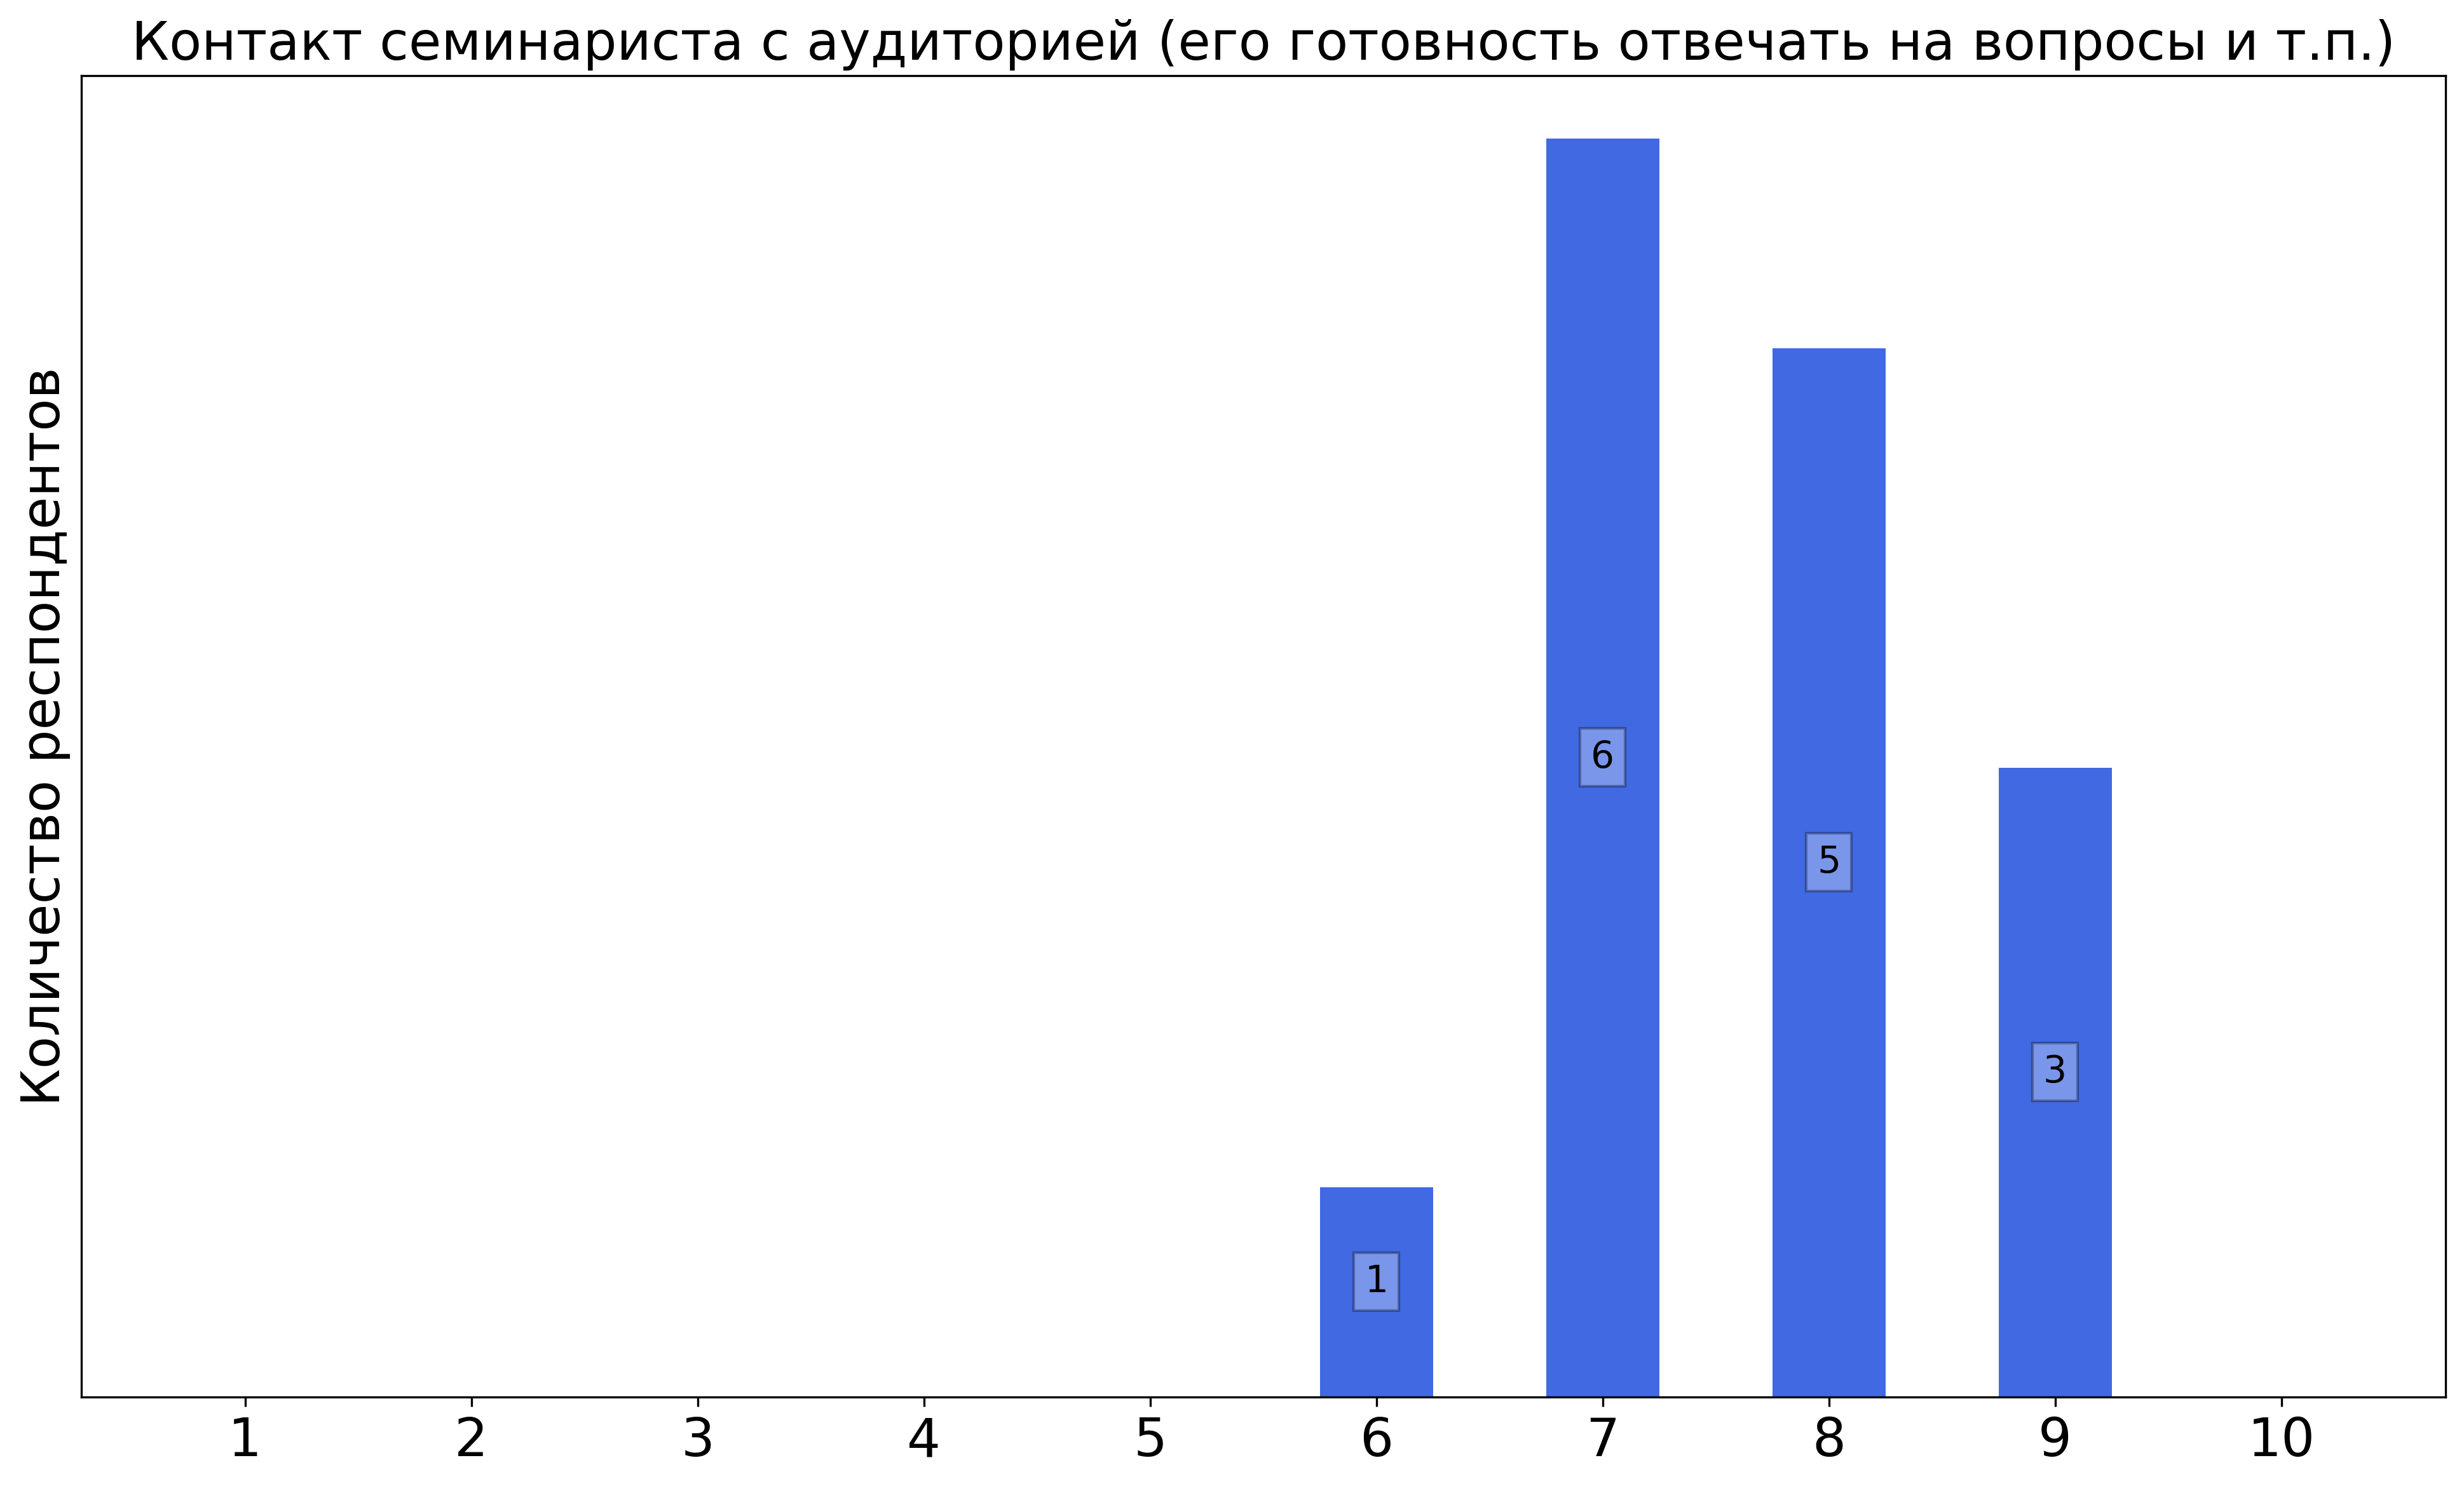
\includegraphics[width=\textwidth]{images/1 course/Общая физика - механика/seminarists-marks-Холин Д.И.-0.png}
			\end{subfigure}
			\begin{subfigure}[b]{0.45\textwidth}
				\centering
				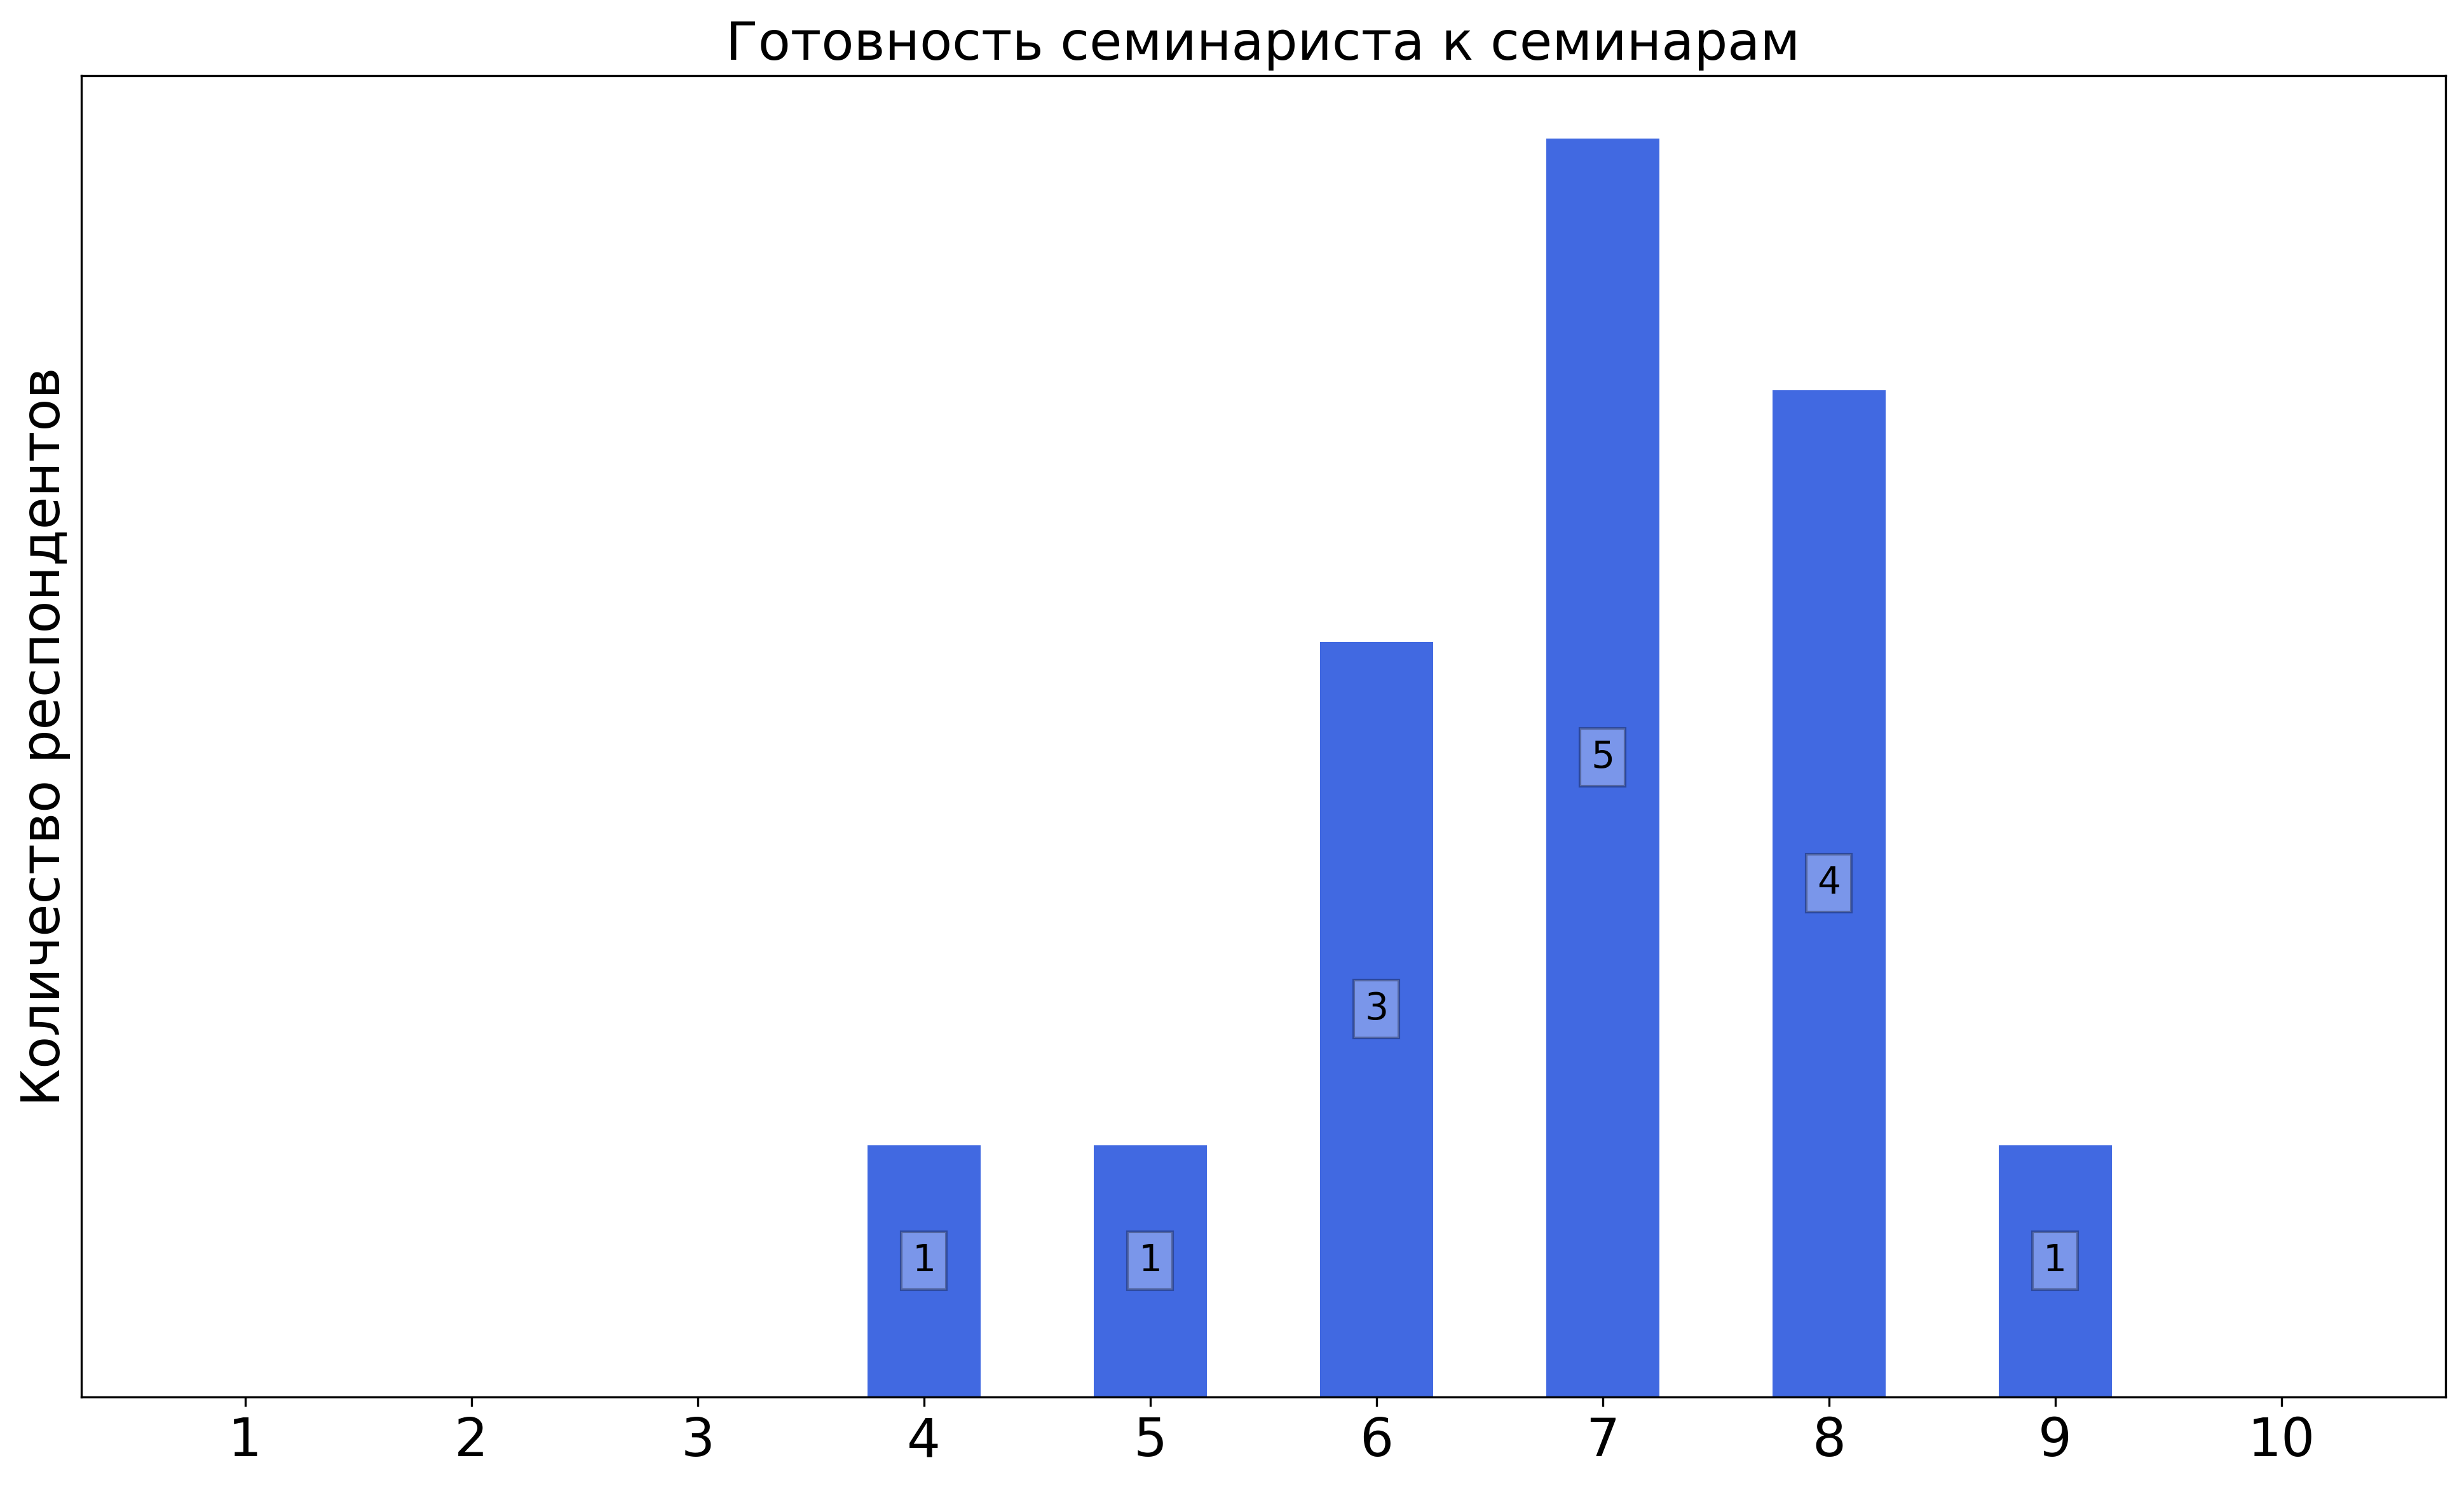
\includegraphics[width=\textwidth]{images/1 course/Общая физика - механика/seminarists-marks-Холин Д.И.-1.png}
			\end{subfigure}
			\begin{subfigure}[b]{0.45\textwidth}
				\centering
				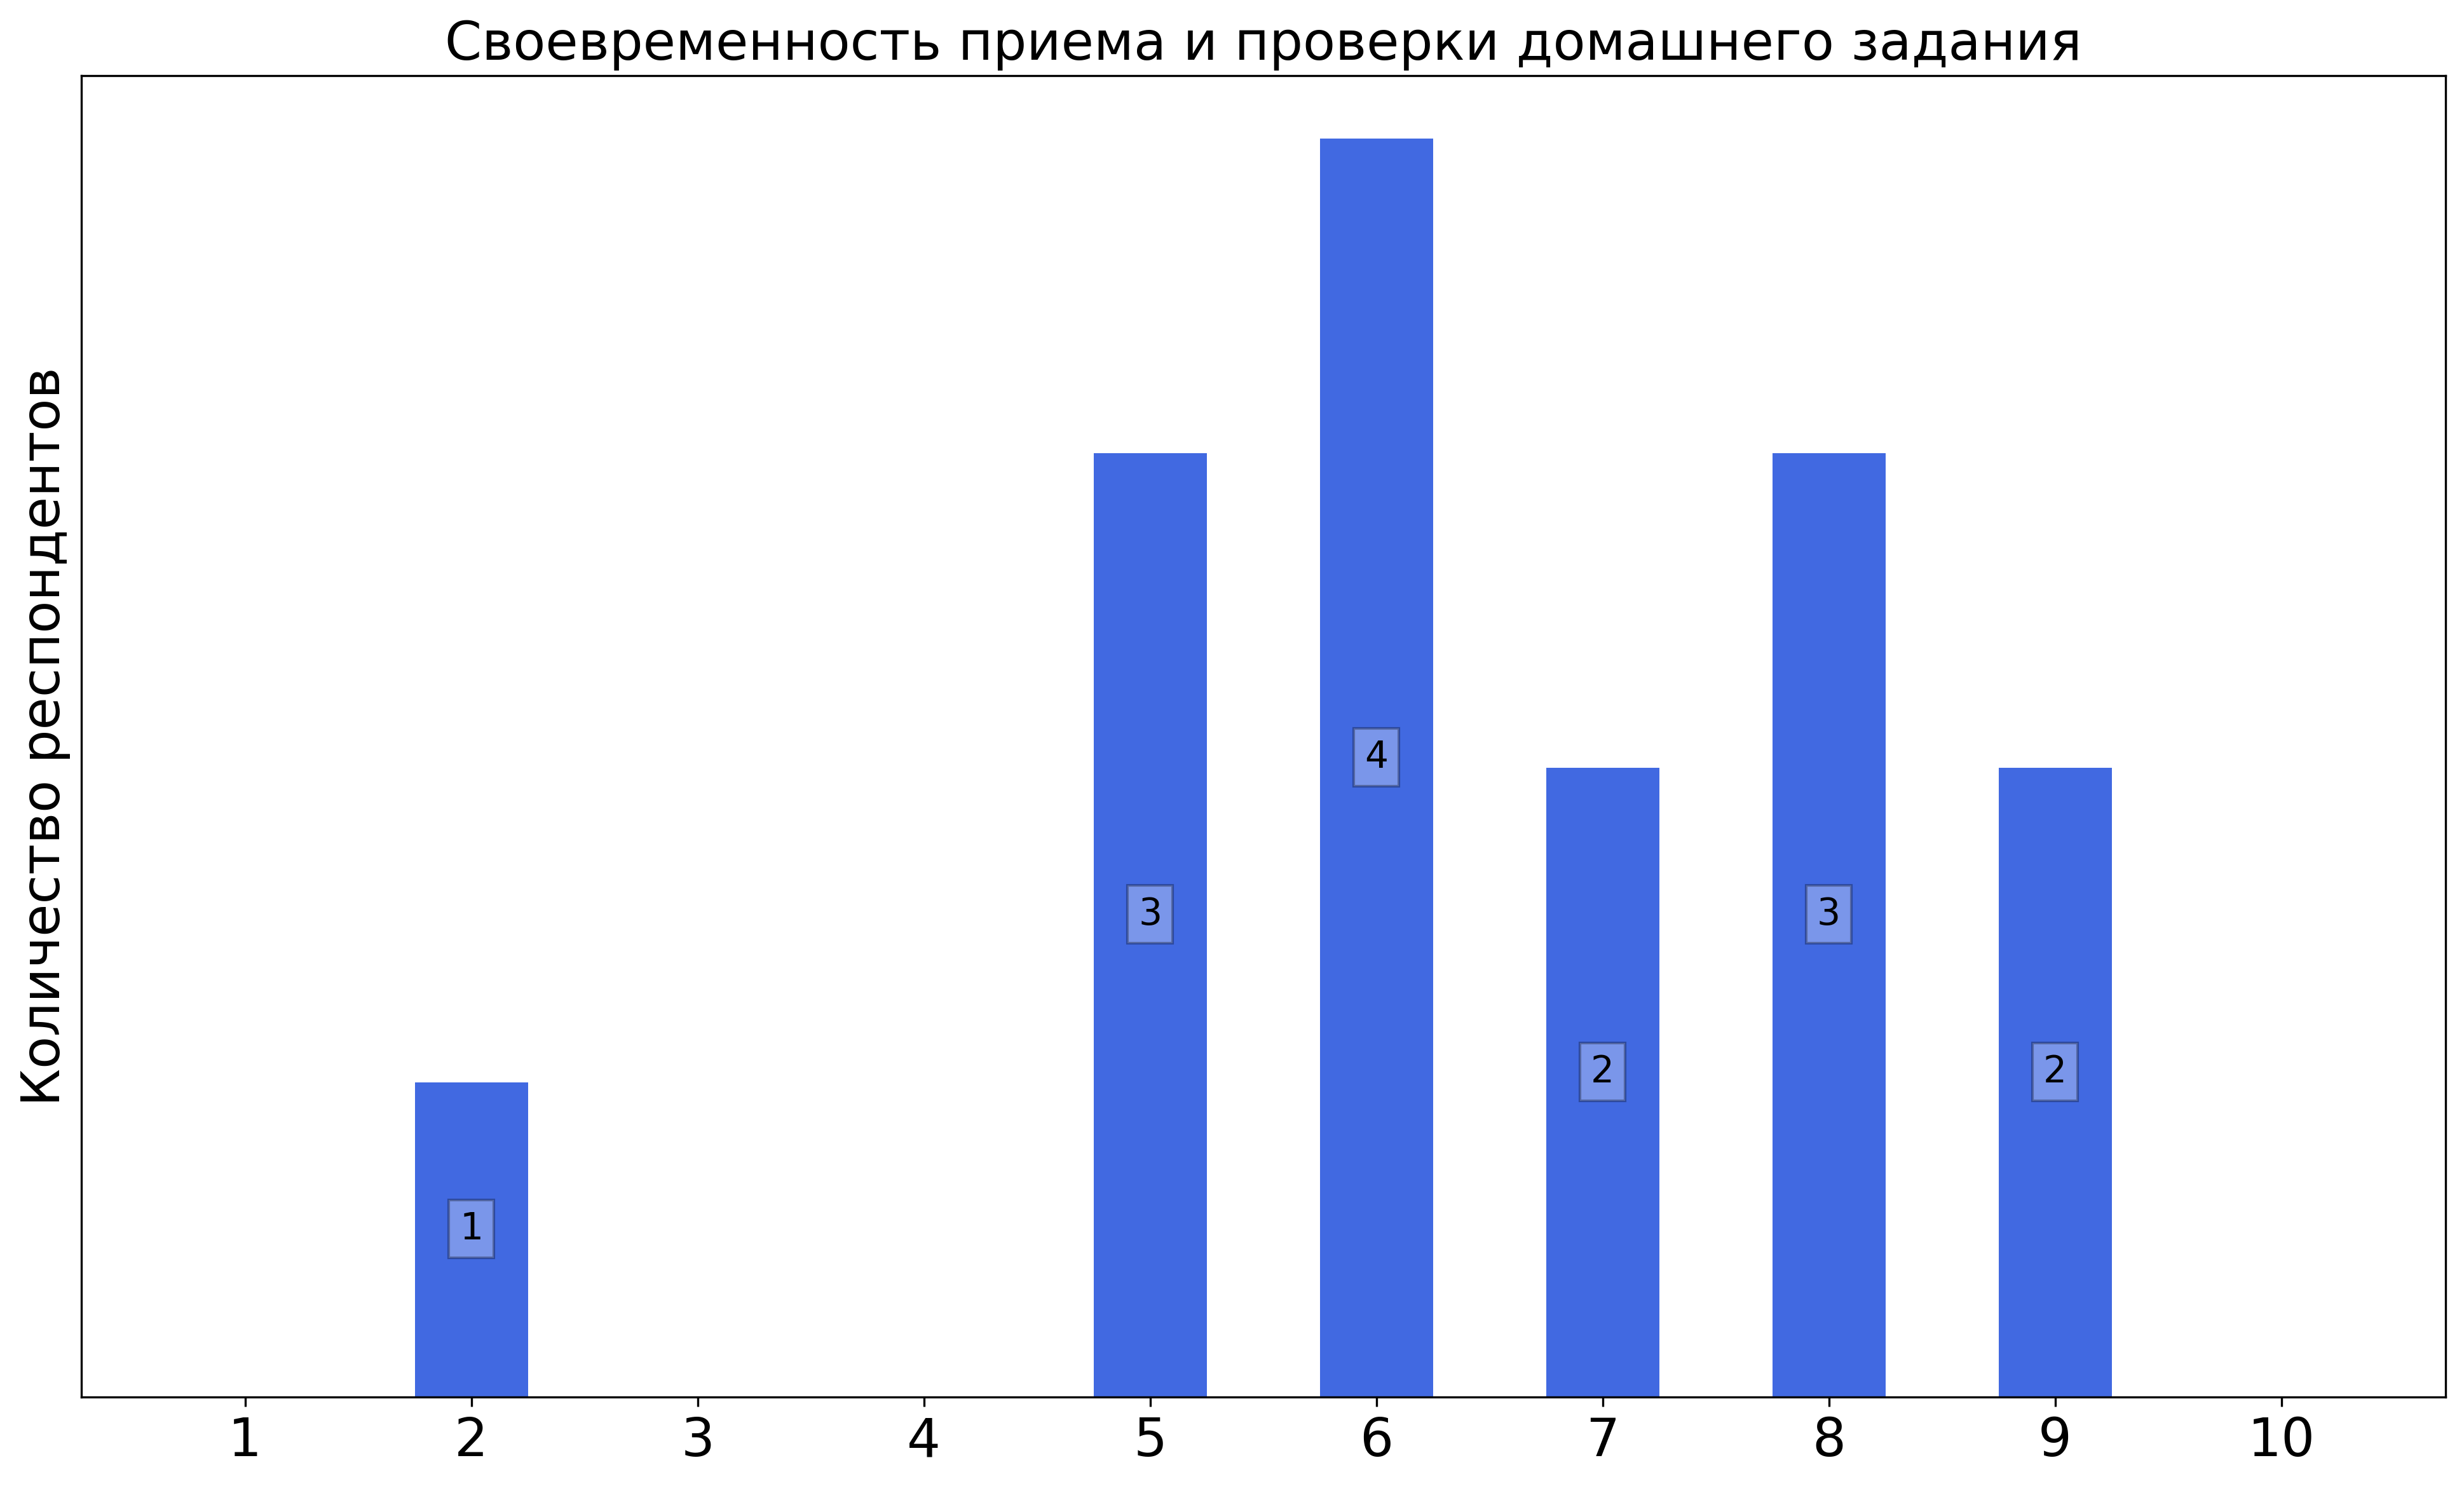
\includegraphics[width=\textwidth]{images/1 course/Общая физика - механика/seminarists-marks-Холин Д.И.-2.png}
			\end{subfigure}
			\begin{subfigure}[b]{0.45\textwidth}
				\centering
				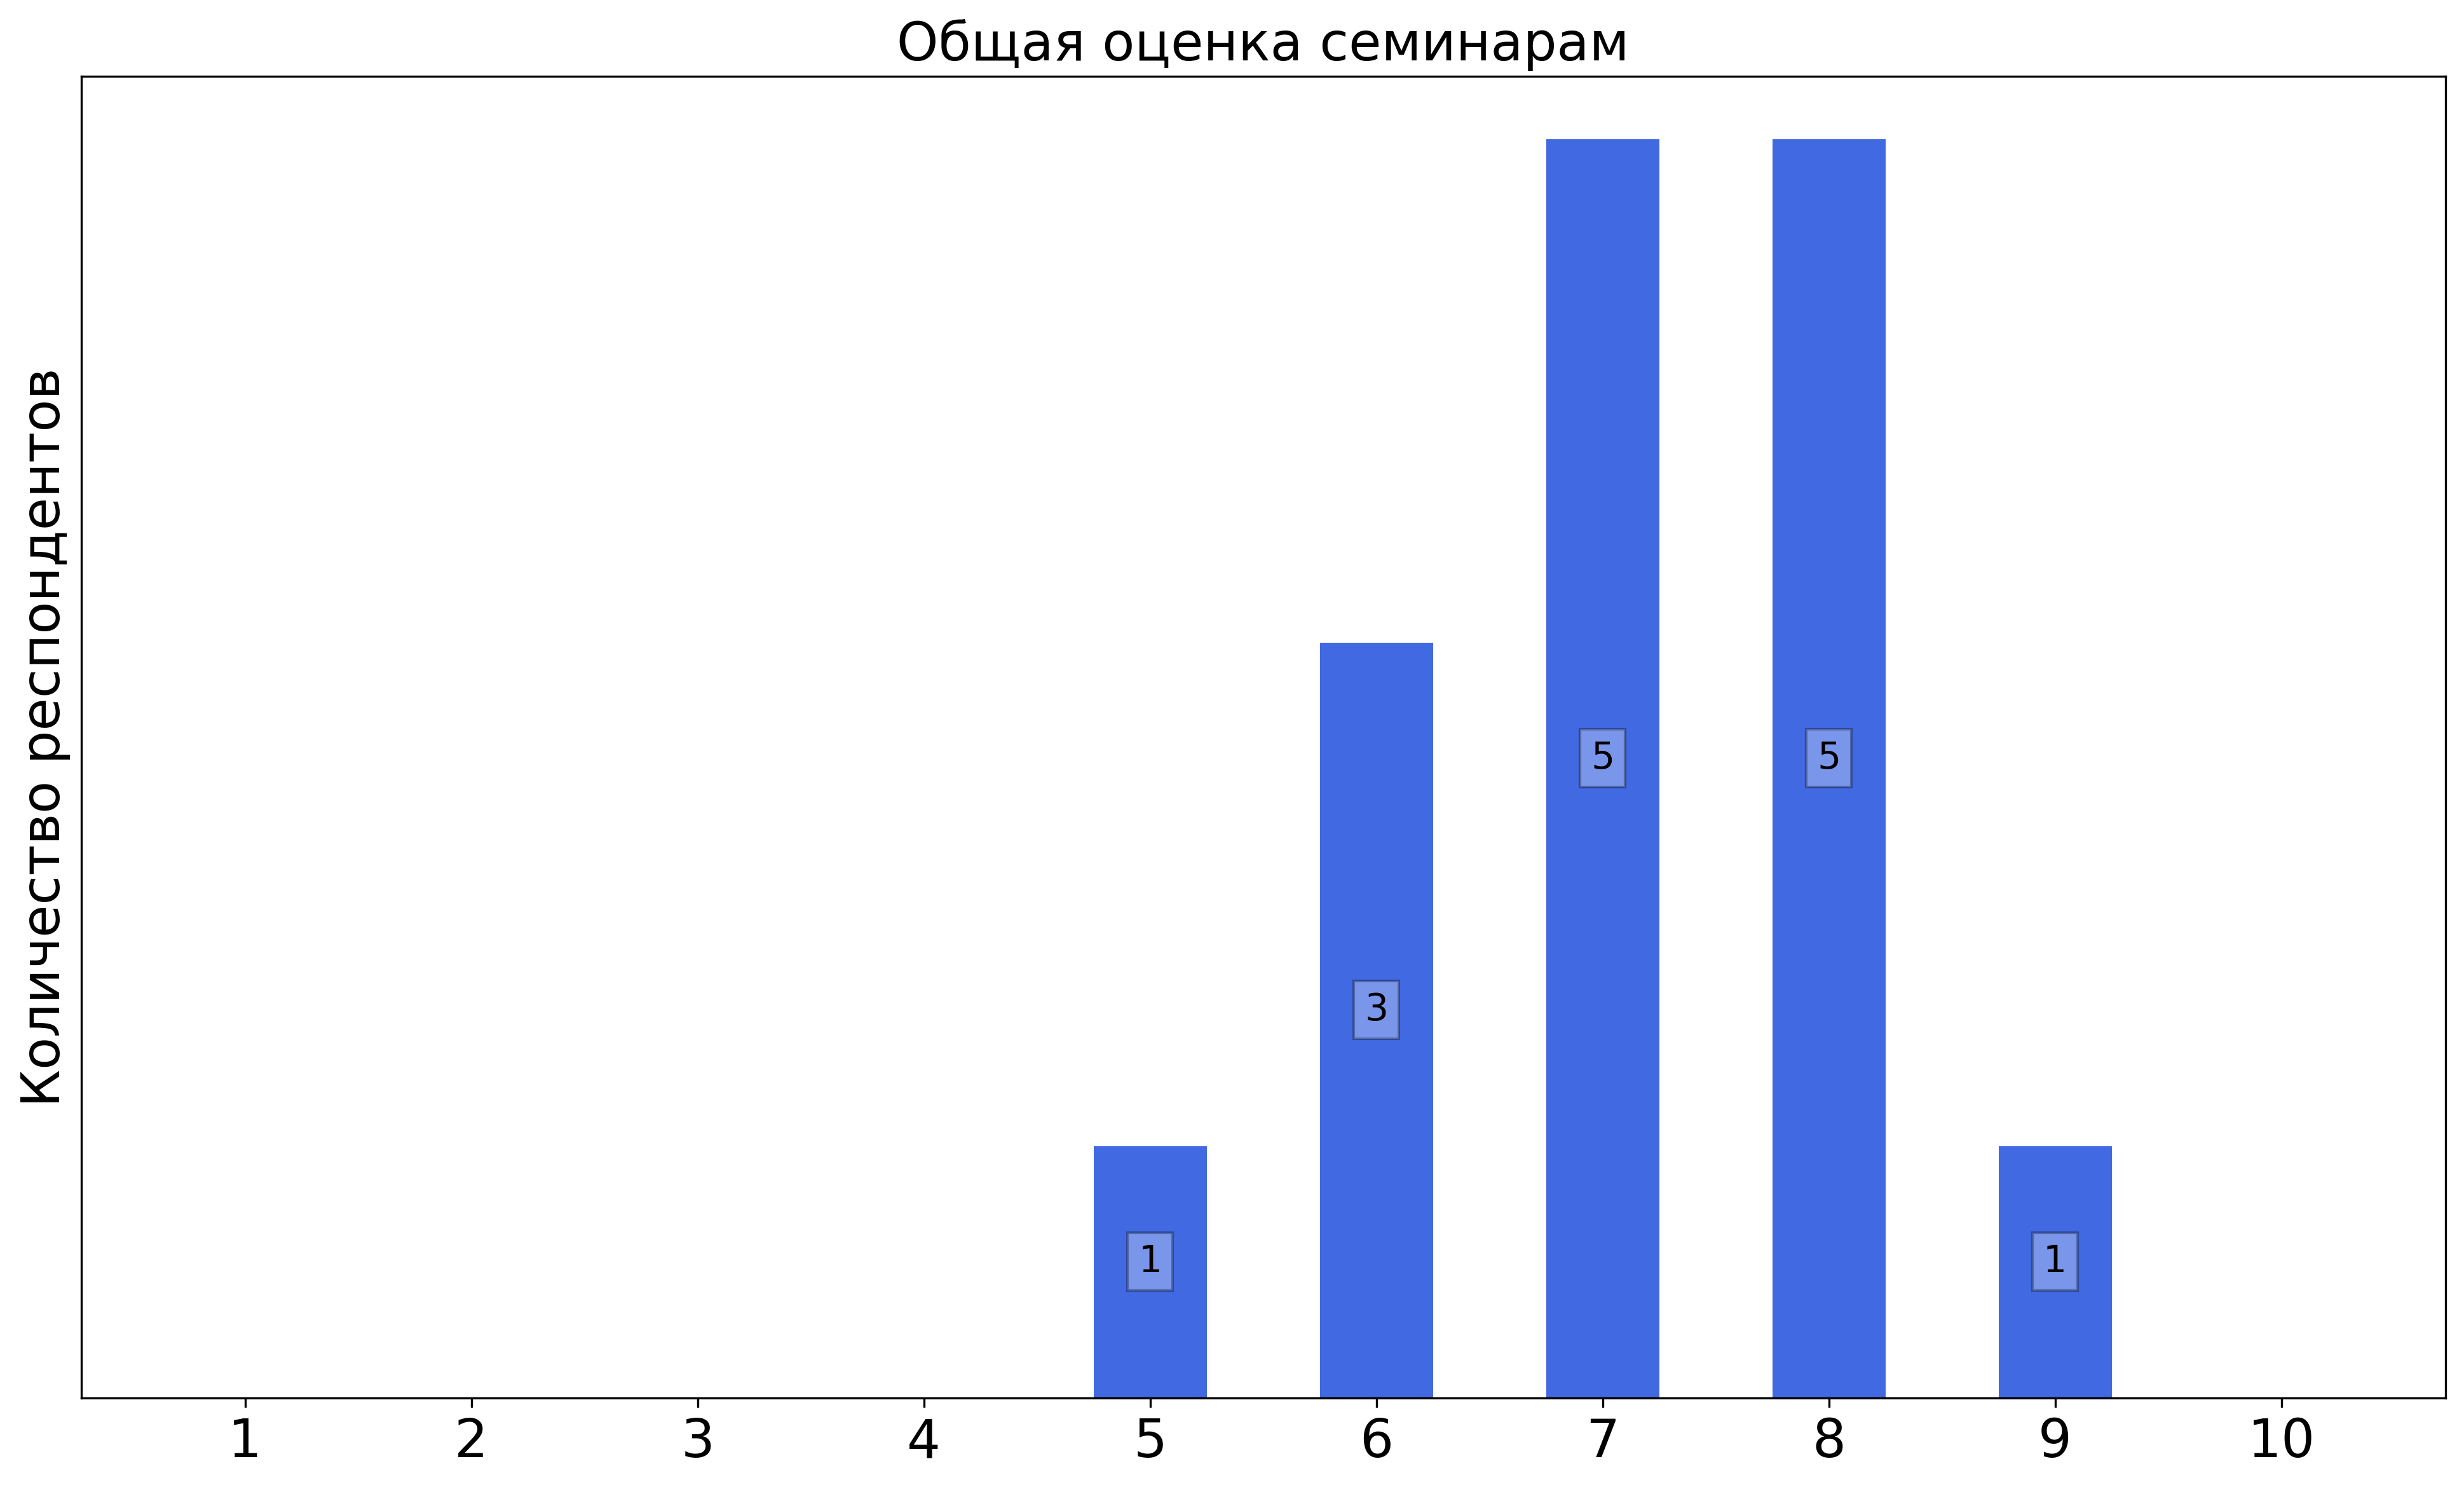
\includegraphics[width=\textwidth]{images/1 course/Общая физика - механика/seminarists-marks-Холин Д.И.-3.png}
			\end{subfigure}	
			\caption{Оценки респондентов о качестве преподавания семинаров}
		\end{figure}

		\textbf{Комментарии студентов о семинаристе\protect\footnote{сохранены оригинальные орфография и пунктуация}}
            \begin{commentbox} 
                Неплохо преподает, однако иногда сам не знает, как решить,но, с другой стороны, получается, что он ВСЕГДА сам действительно придумает решение задачи, а, значит, и объяснить его 
            \end{commentbox} 
        
            \begin{commentbox} 
                Отличный семинарист, мне все по кайфу 
            \end{commentbox} 
        
            \begin{commentbox} 
                Хороший семинарист. Хочет докопаться до истины, а не добиться того, чтобы кто-то записал правильное решение на доске. Часто предлагает более простые решения, но и не полениться довести  до конца сложные. 
            \end{commentbox} 
        
            \begin{commentbox} 
                С данным семинаристом критерий готовность к семинарам сомнительный. Так как на них сами студенты разбирали задачи, преподаватель буквально пару раз за пару мог что то пояснить или сказать 
            \end{commentbox} 
        
            \begin{commentbox} 
                Хорошо объясняются методы решения задач, рассматриваются альтернативные варианты решения. Творческий подход 
            \end{commentbox} 
        
            \begin{commentbox} 
                Нулёвки сдаются на листочке в начале семинара, единички рассказывают друг другу студенты, при этом Д. И. вносит свои комментарии, иногда показывает другие интересные пути решения задач.Такой формат проведения семинаров меня вполне устраивает. Минусы: почти всегда не успеваем разобрать все единички, а если если плохо шаришь, то ДЗ может принимать очень долго (некоторые сдавали первое ДЗ в конце семестра).   
            \end{commentbox}
    
    
    \subsubsection{Отзыв студентов о семинарах. Семинарист: Чивелев В.И.}
        \begin{figure}[H]
            \centering
            \begin{subfigure}[b]{0.45\textwidth}
                \centering
                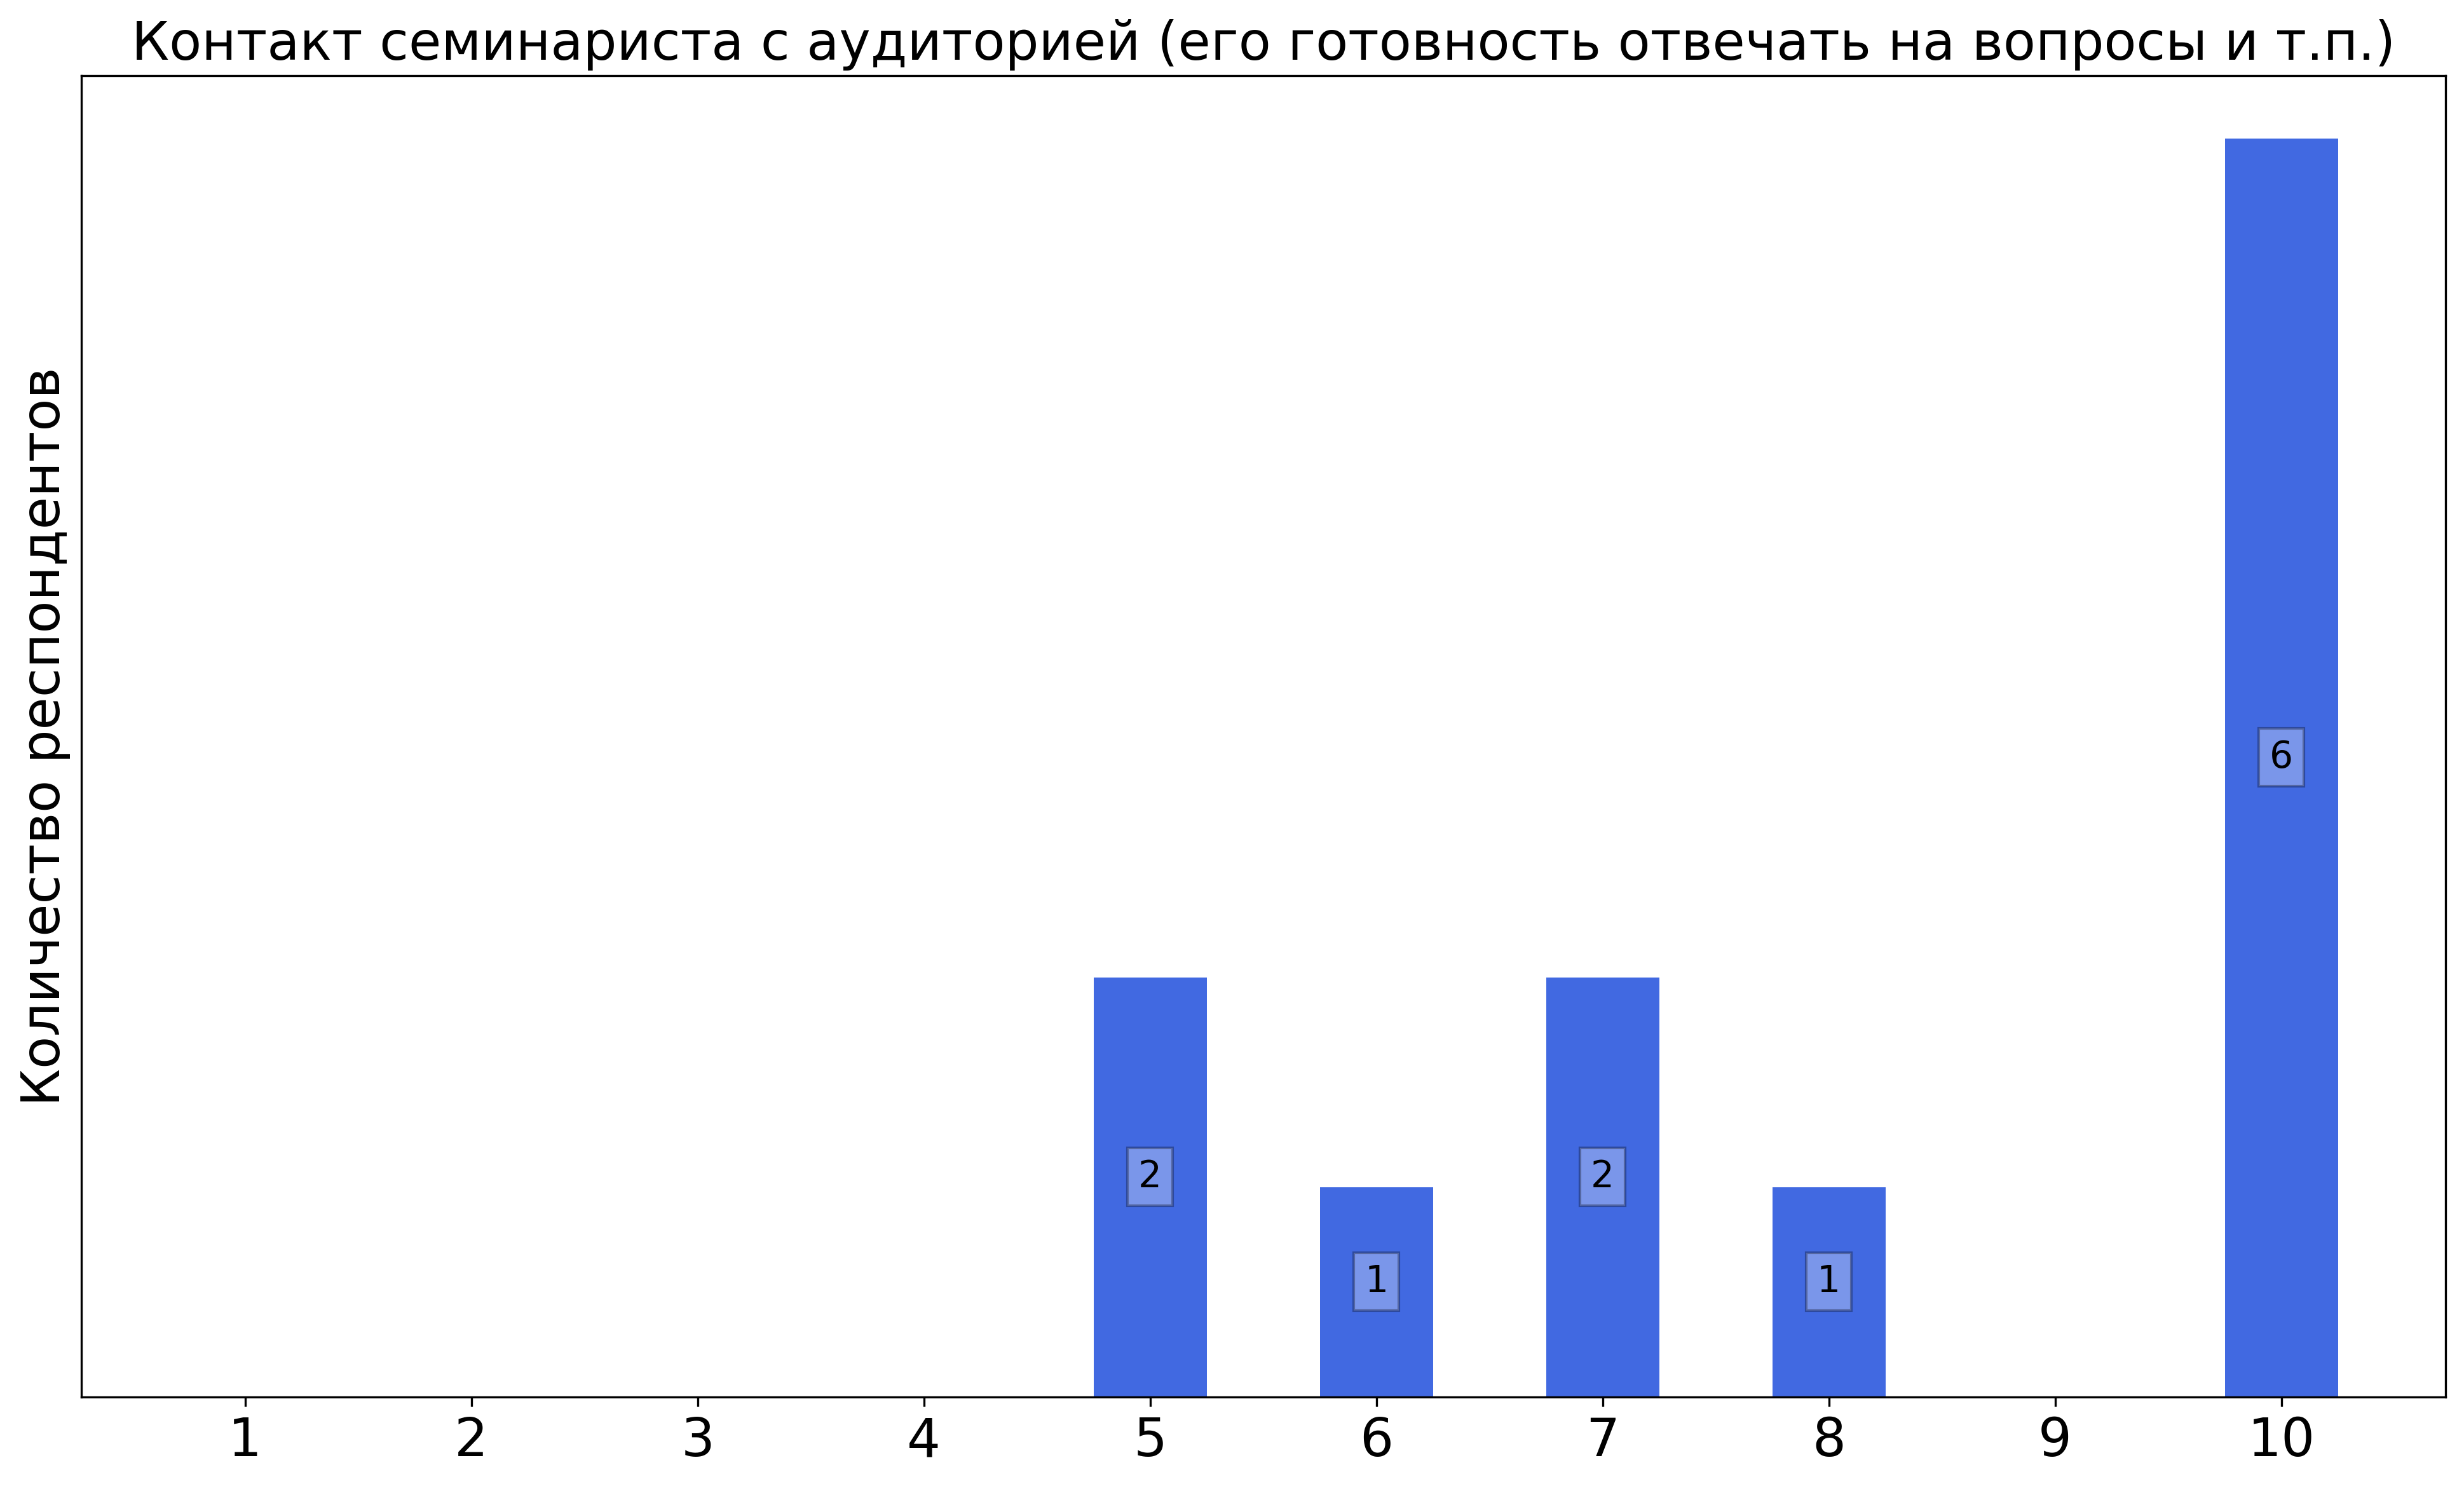
\includegraphics[width=\textwidth]{images/1 course/Общая физика - механика/seminarists-marks-Чивелев В.И.-0.png}
            \end{subfigure}
            \begin{subfigure}[b]{0.45\textwidth}
                \centering
                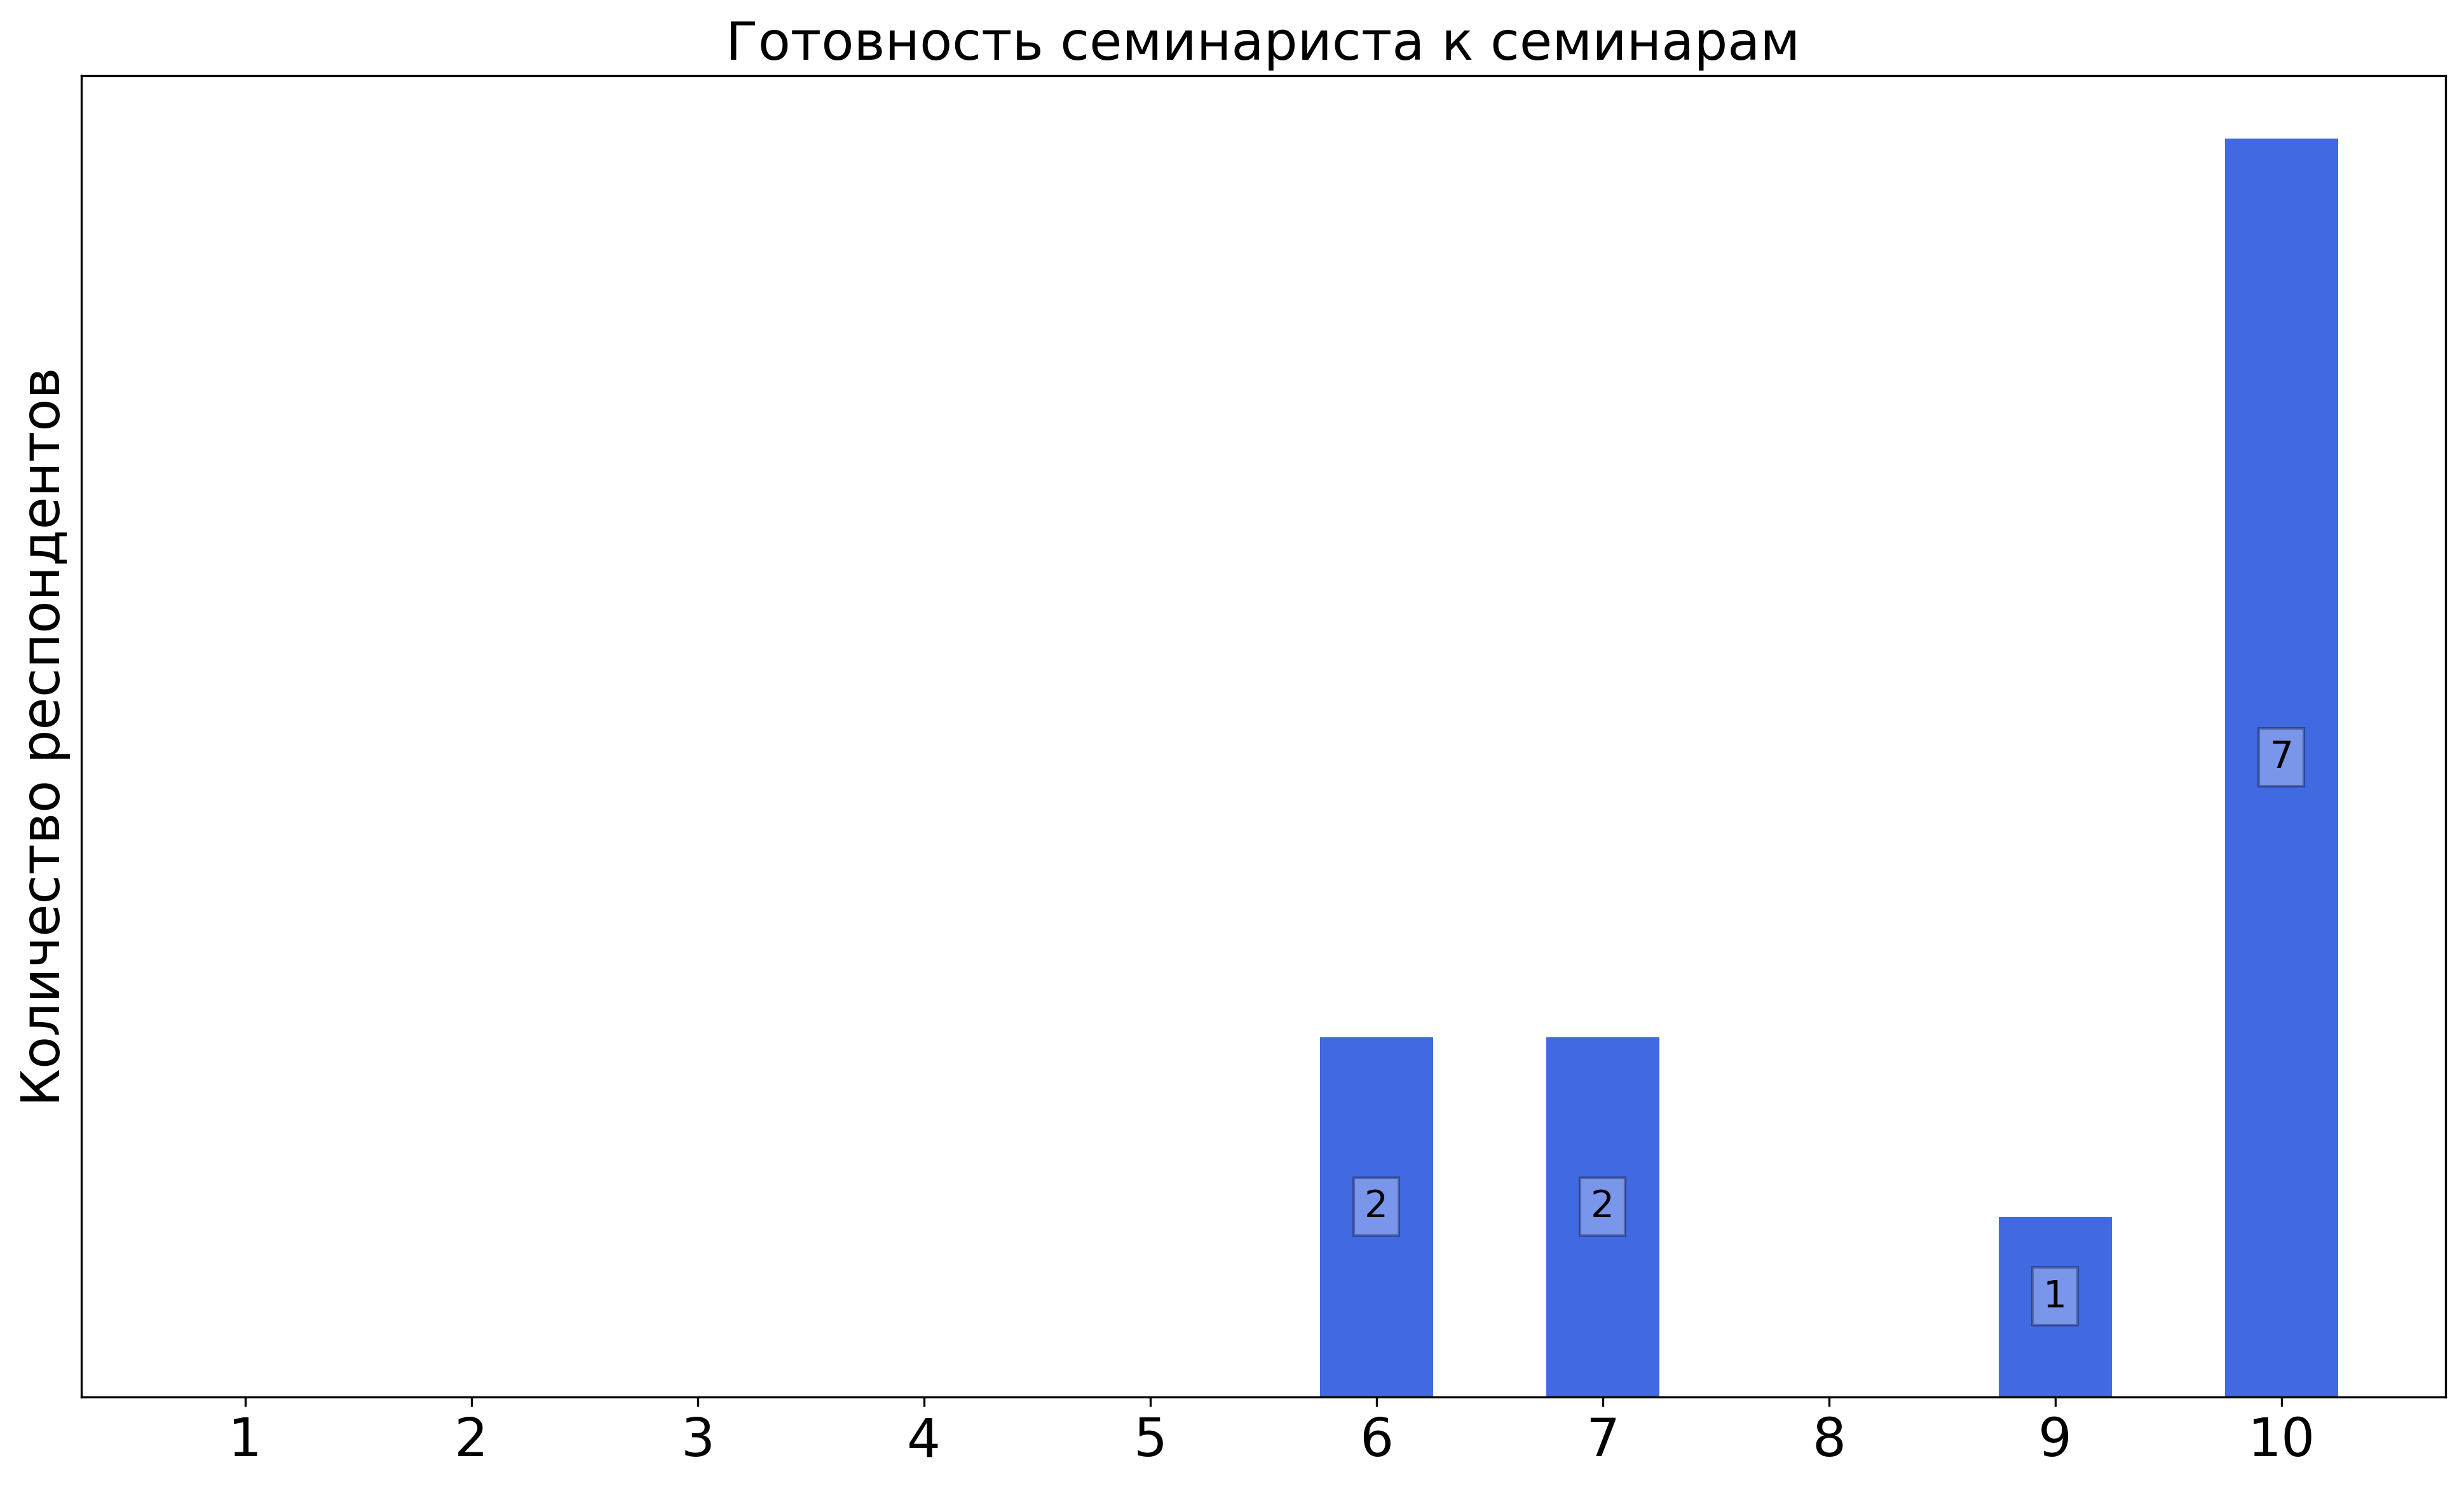
\includegraphics[width=\textwidth]{images/1 course/Общая физика - механика/seminarists-marks-Чивелев В.И.-1.png}
            \end{subfigure}
            \begin{subfigure}[b]{0.45\textwidth}
                \centering
                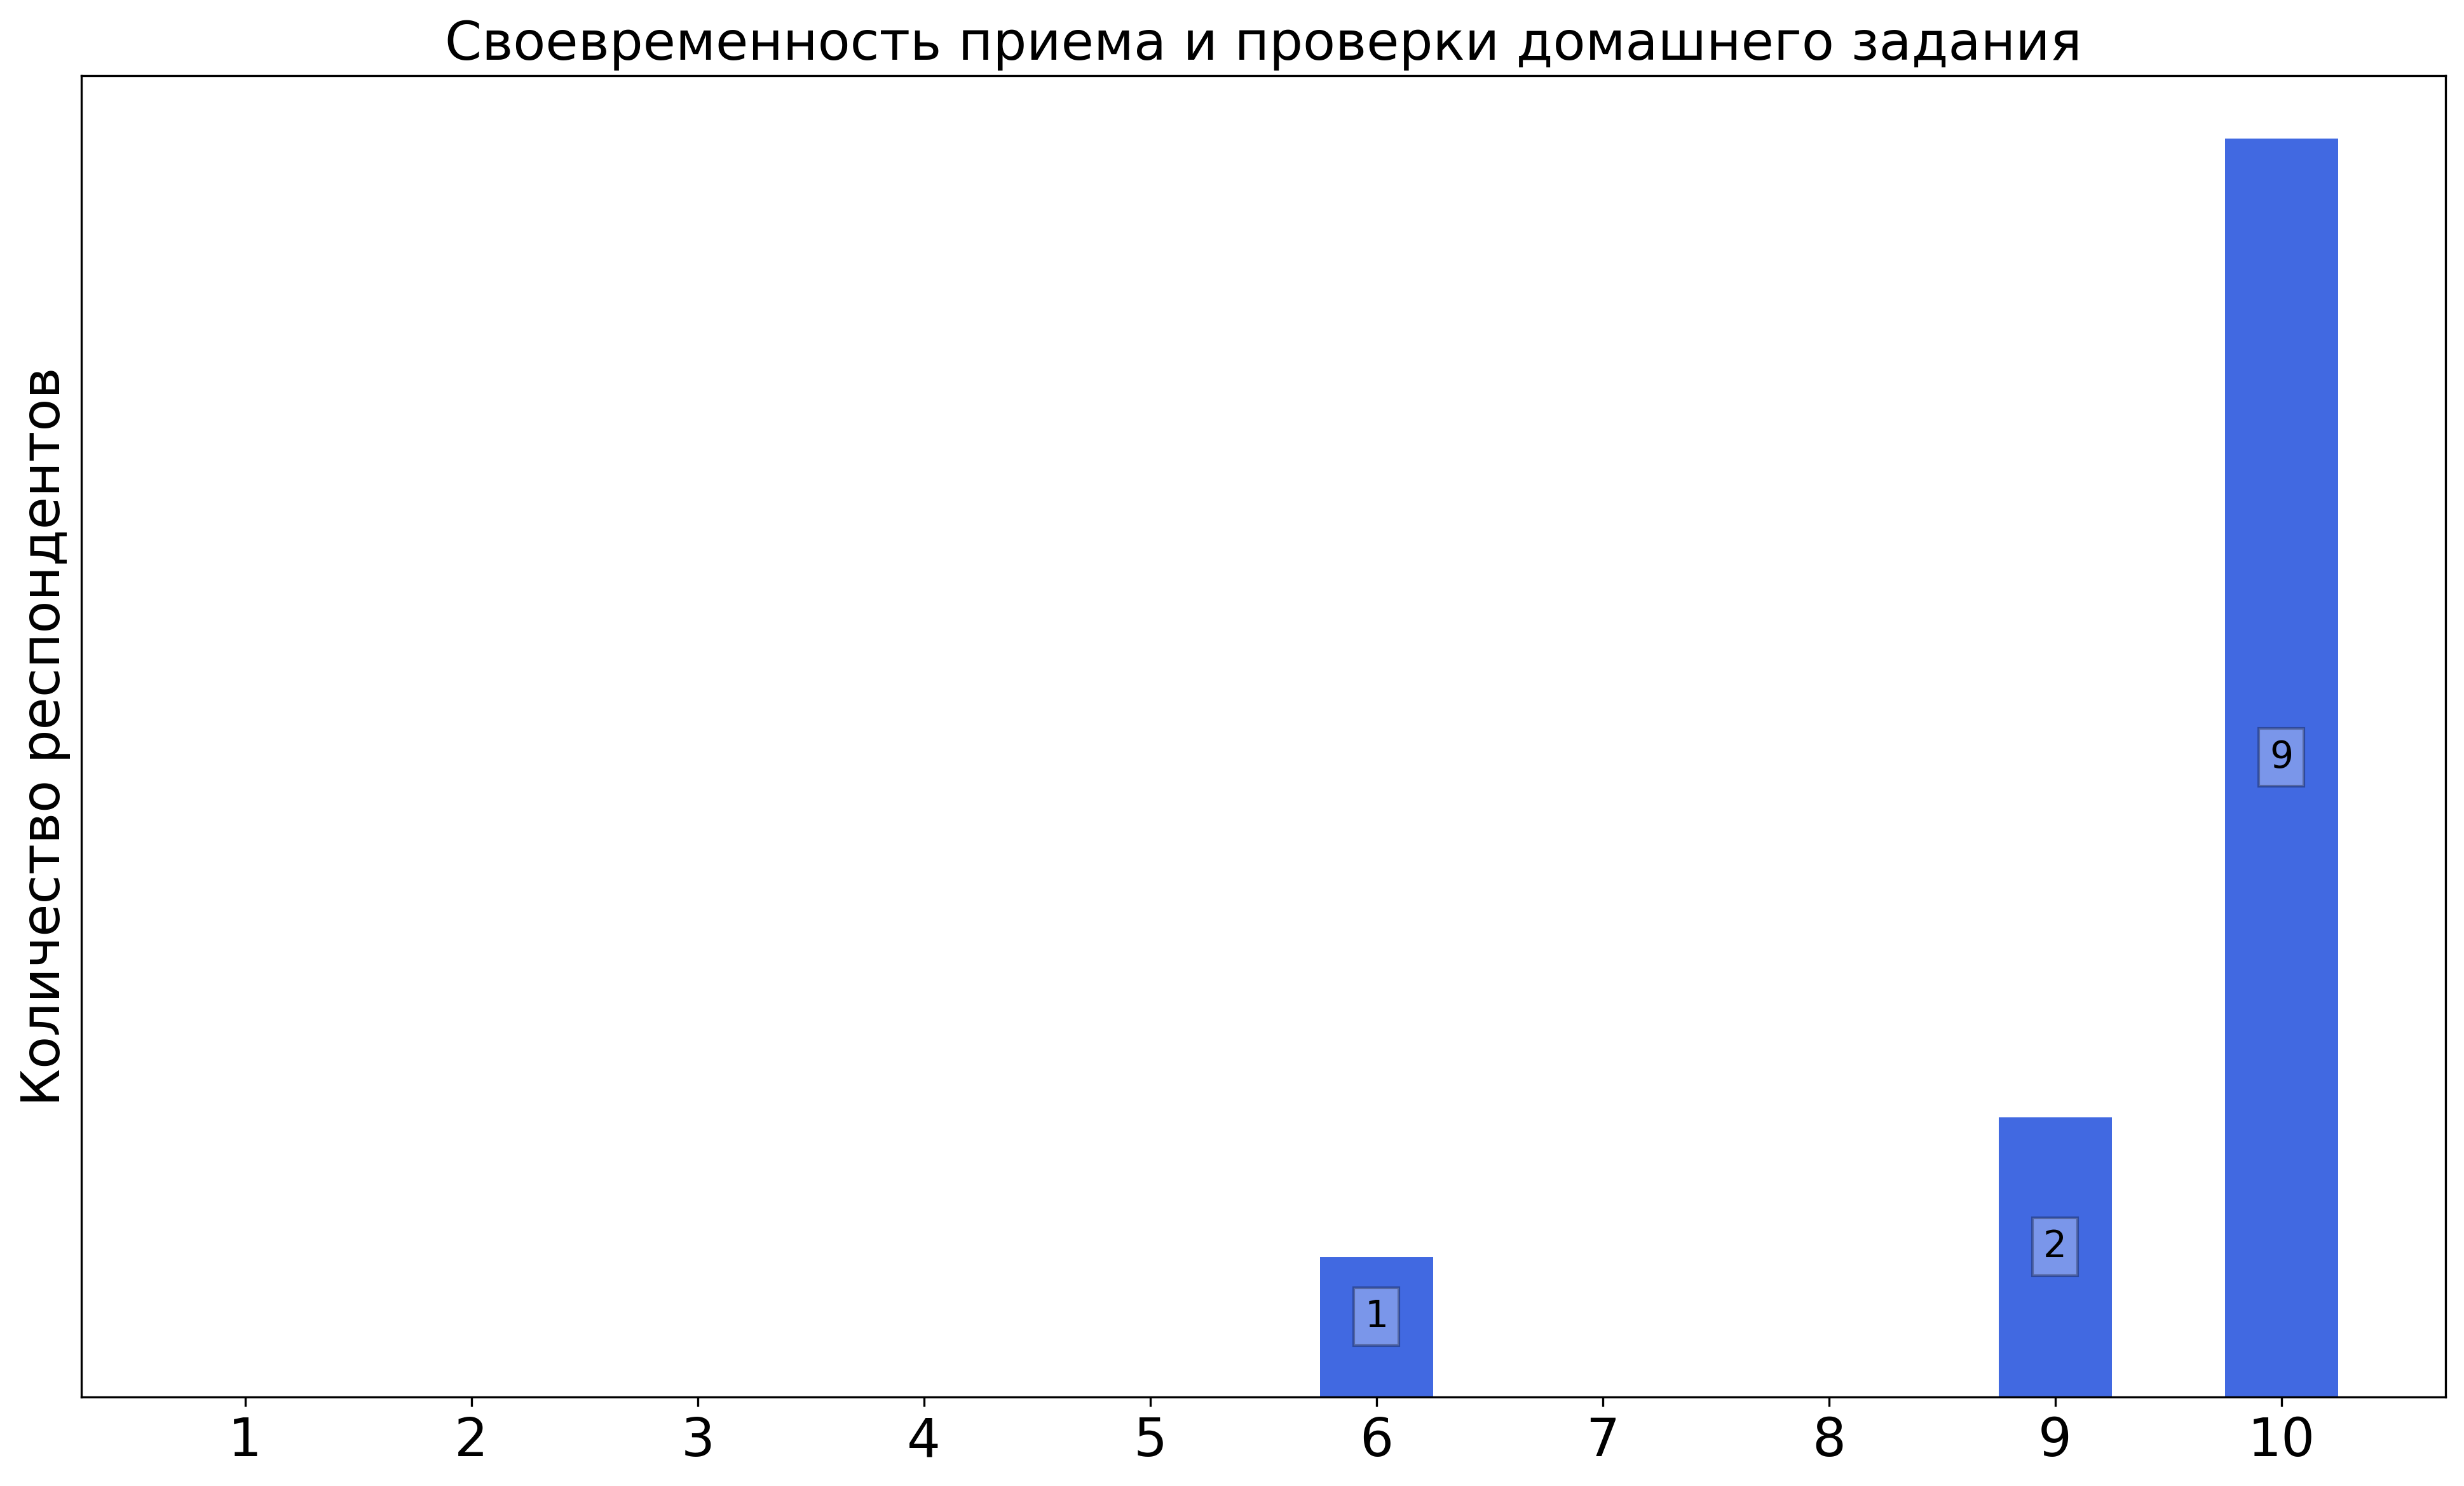
\includegraphics[width=\textwidth]{images/1 course/Общая физика - механика/seminarists-marks-Чивелев В.И.-2.png}
            \end{subfigure}
            \begin{subfigure}[b]{0.45\textwidth}
                \centering
                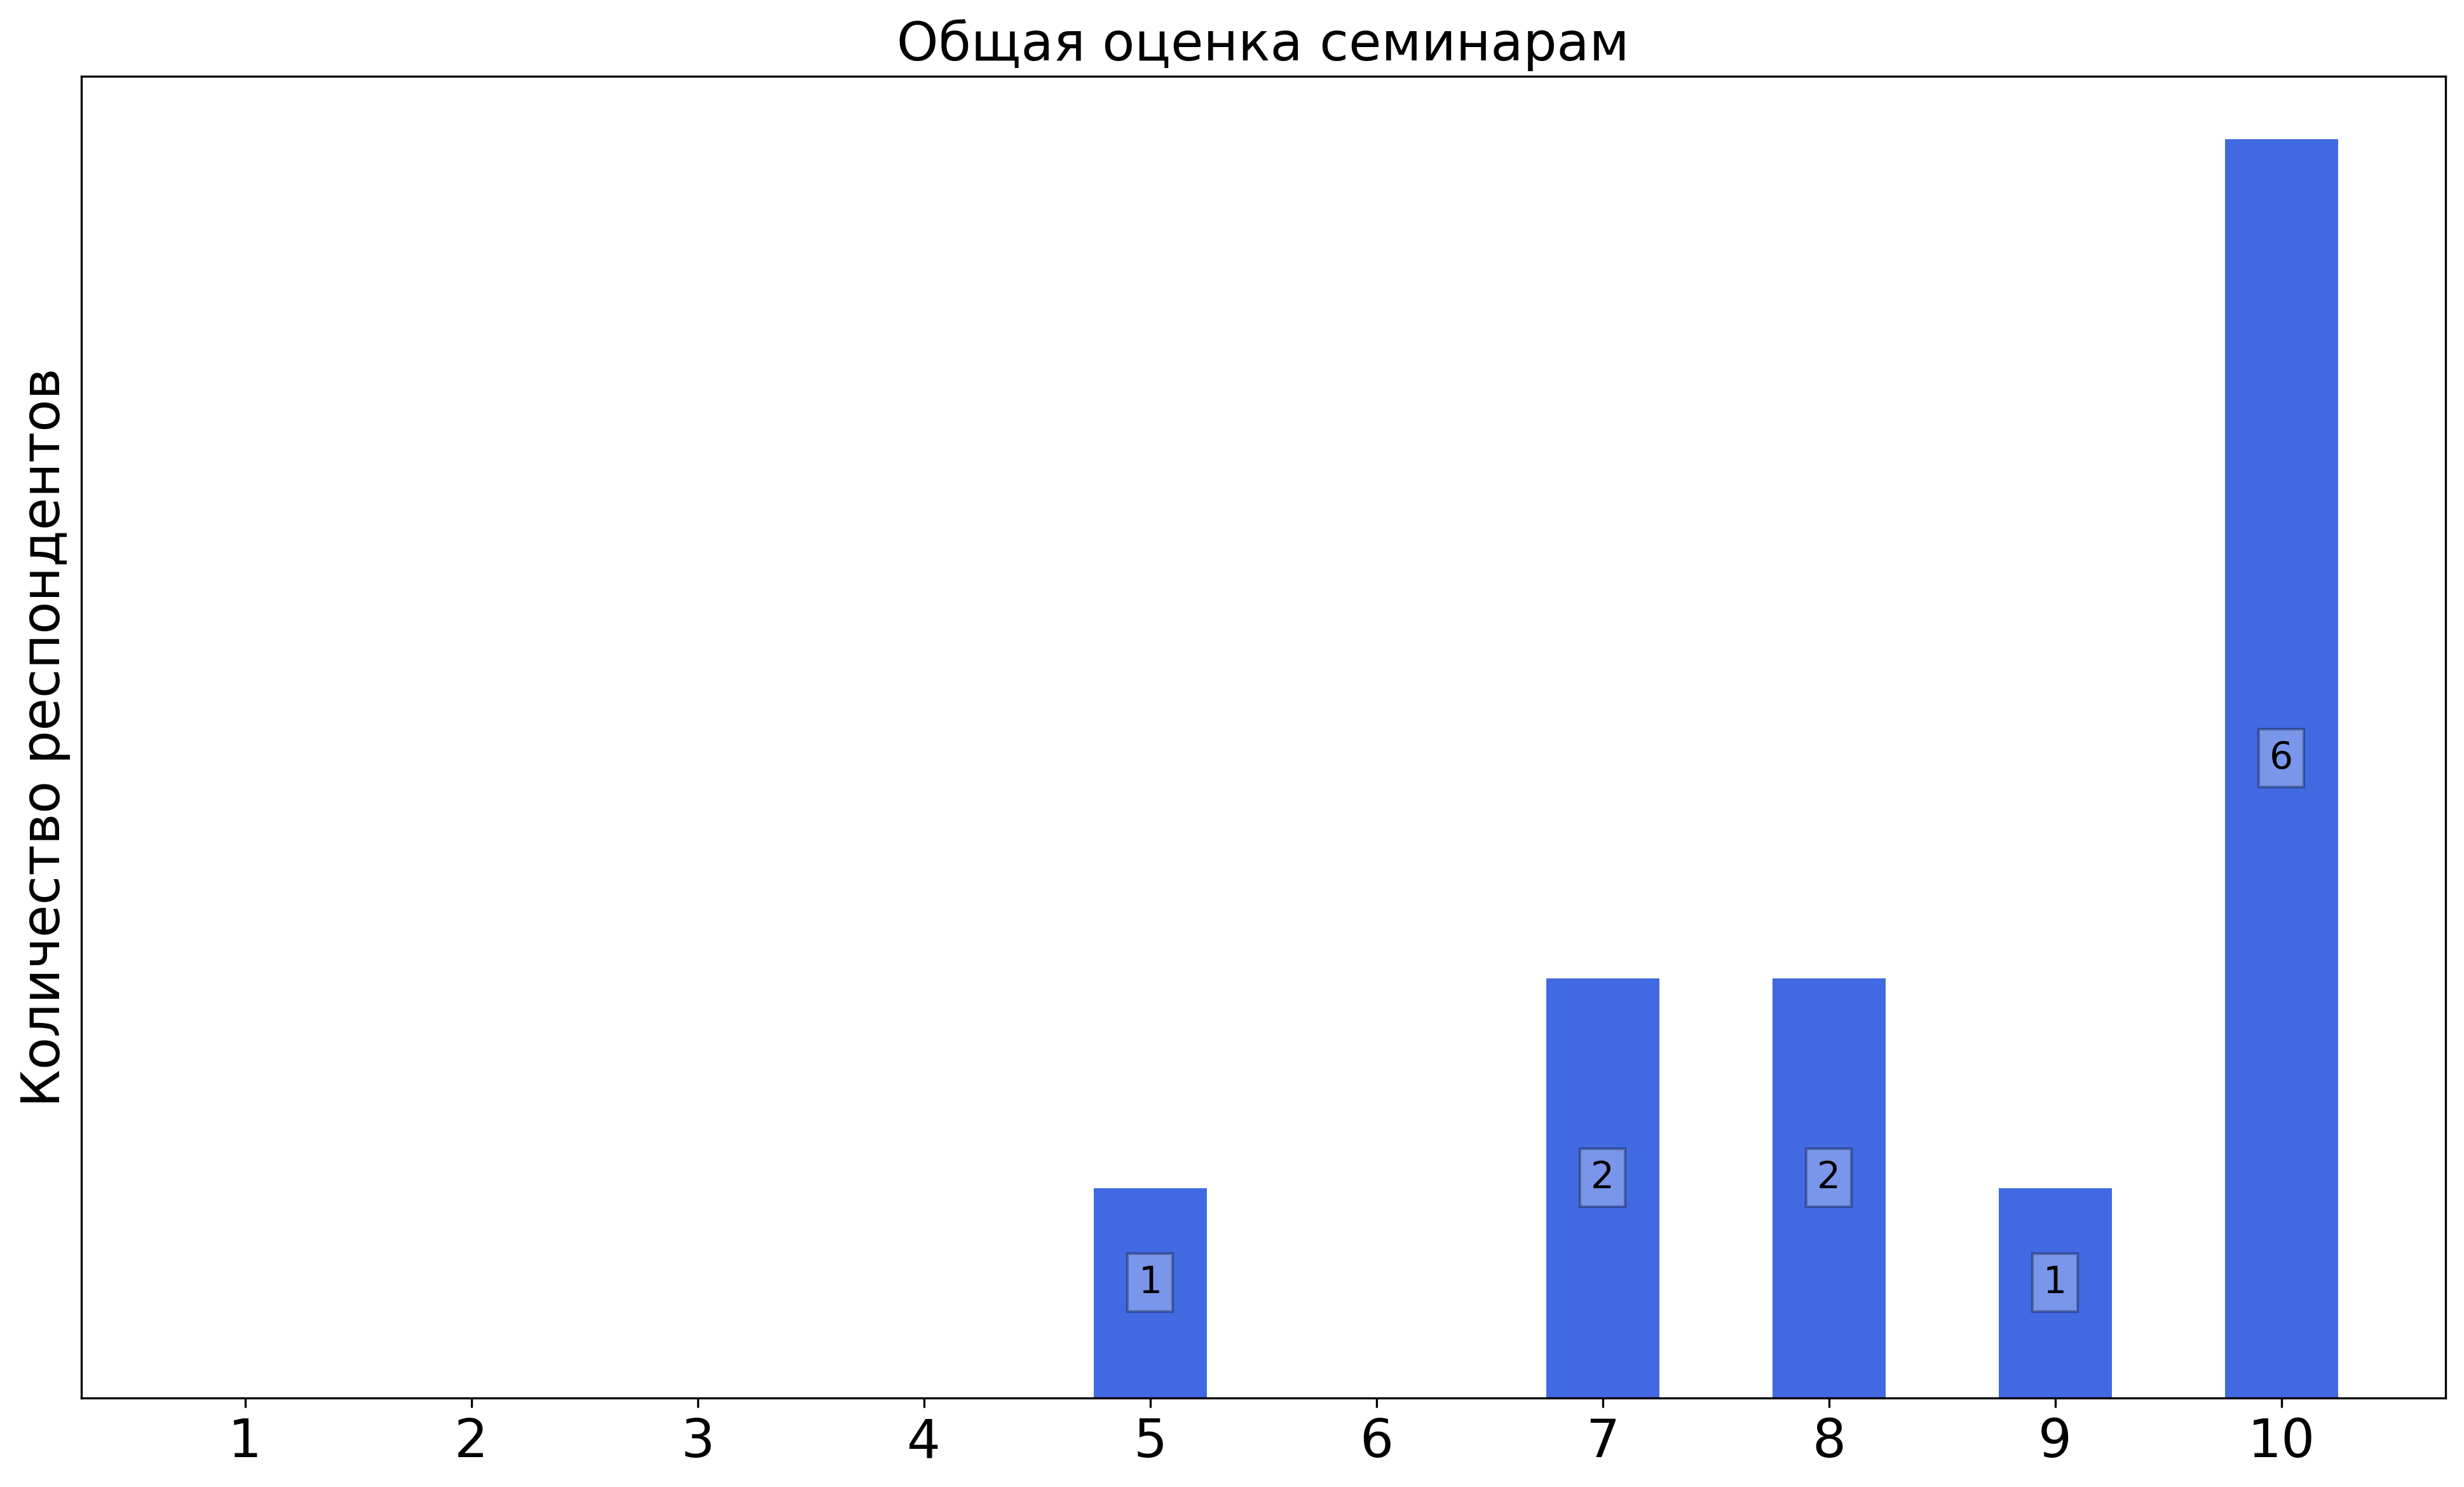
\includegraphics[width=\textwidth]{images/1 course/Общая физика - механика/seminarists-marks-Чивелев В.И.-3.png}
            \end{subfigure}	
            \caption{Оценки респондентов о качестве преподавания семинаров}
        \end{figure}

        \textbf{Комментарии студентов о семинаристе\protect\footnote{сохранены оригинальные орфография и пунктуация}}
            \begin{commentbox} 
                Круто объясняет теорию на семинарах. Дает много Советов по подготовке. 
            \end{commentbox} 
        
            \begin{commentbox} 
                Занижает оценку  
            \end{commentbox} 
        
            \begin{commentbox} 
                неплох, но мало полезного даёт, плюс решает нулёвки на семинарах 
            \end{commentbox} 
        
            \begin{commentbox} 
                отличный семинарист, хочет научить, а не просто рассказать, его отношение к чертежам - это отдельная история 
            \end{commentbox}


    \subsubsection{Отзыв студентов о лабораторных работах. Преподаватель: Веревочкин Ю.Г.}
        \begin{figure}[H]
            \centering
            \begin{subfigure}[b]{0.45\textwidth}
                \centering
                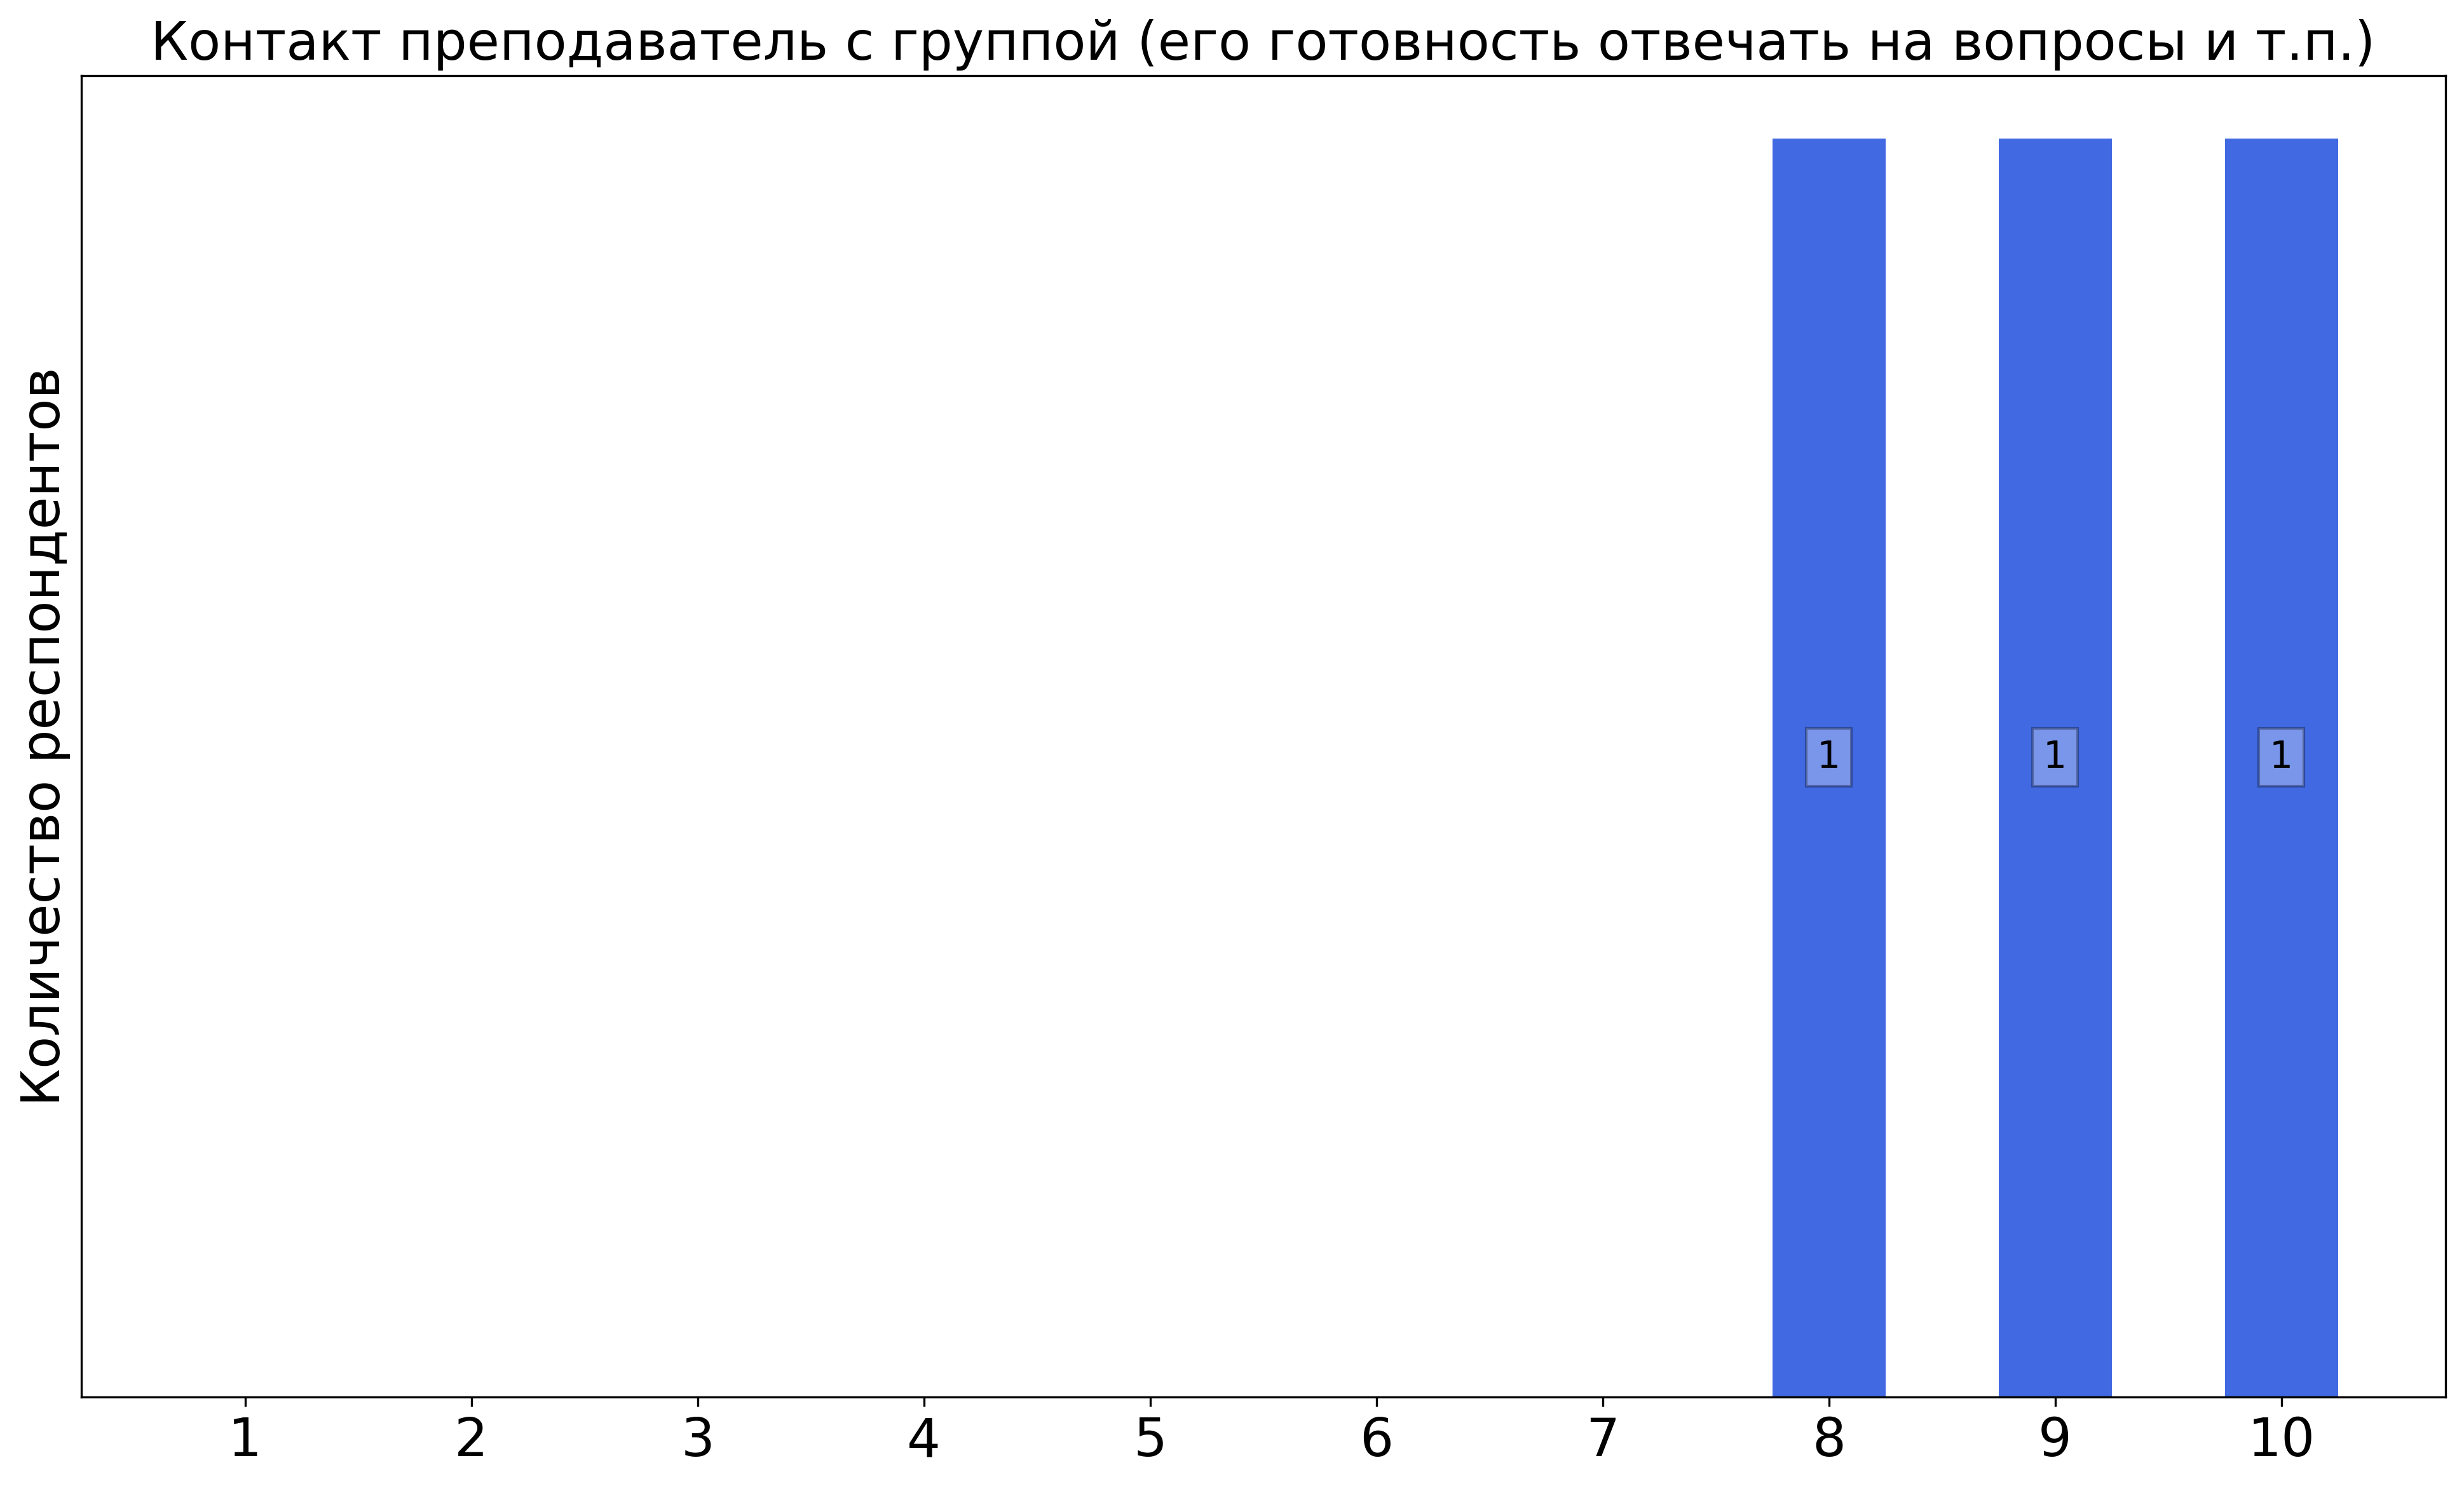
\includegraphics[width=\textwidth]{images/1 course/Общая физика - механика/labniks-marks-Веревочкин Ю.Г.-0.png}
            \end{subfigure}
            \begin{subfigure}[b]{0.45\textwidth}
                \centering
                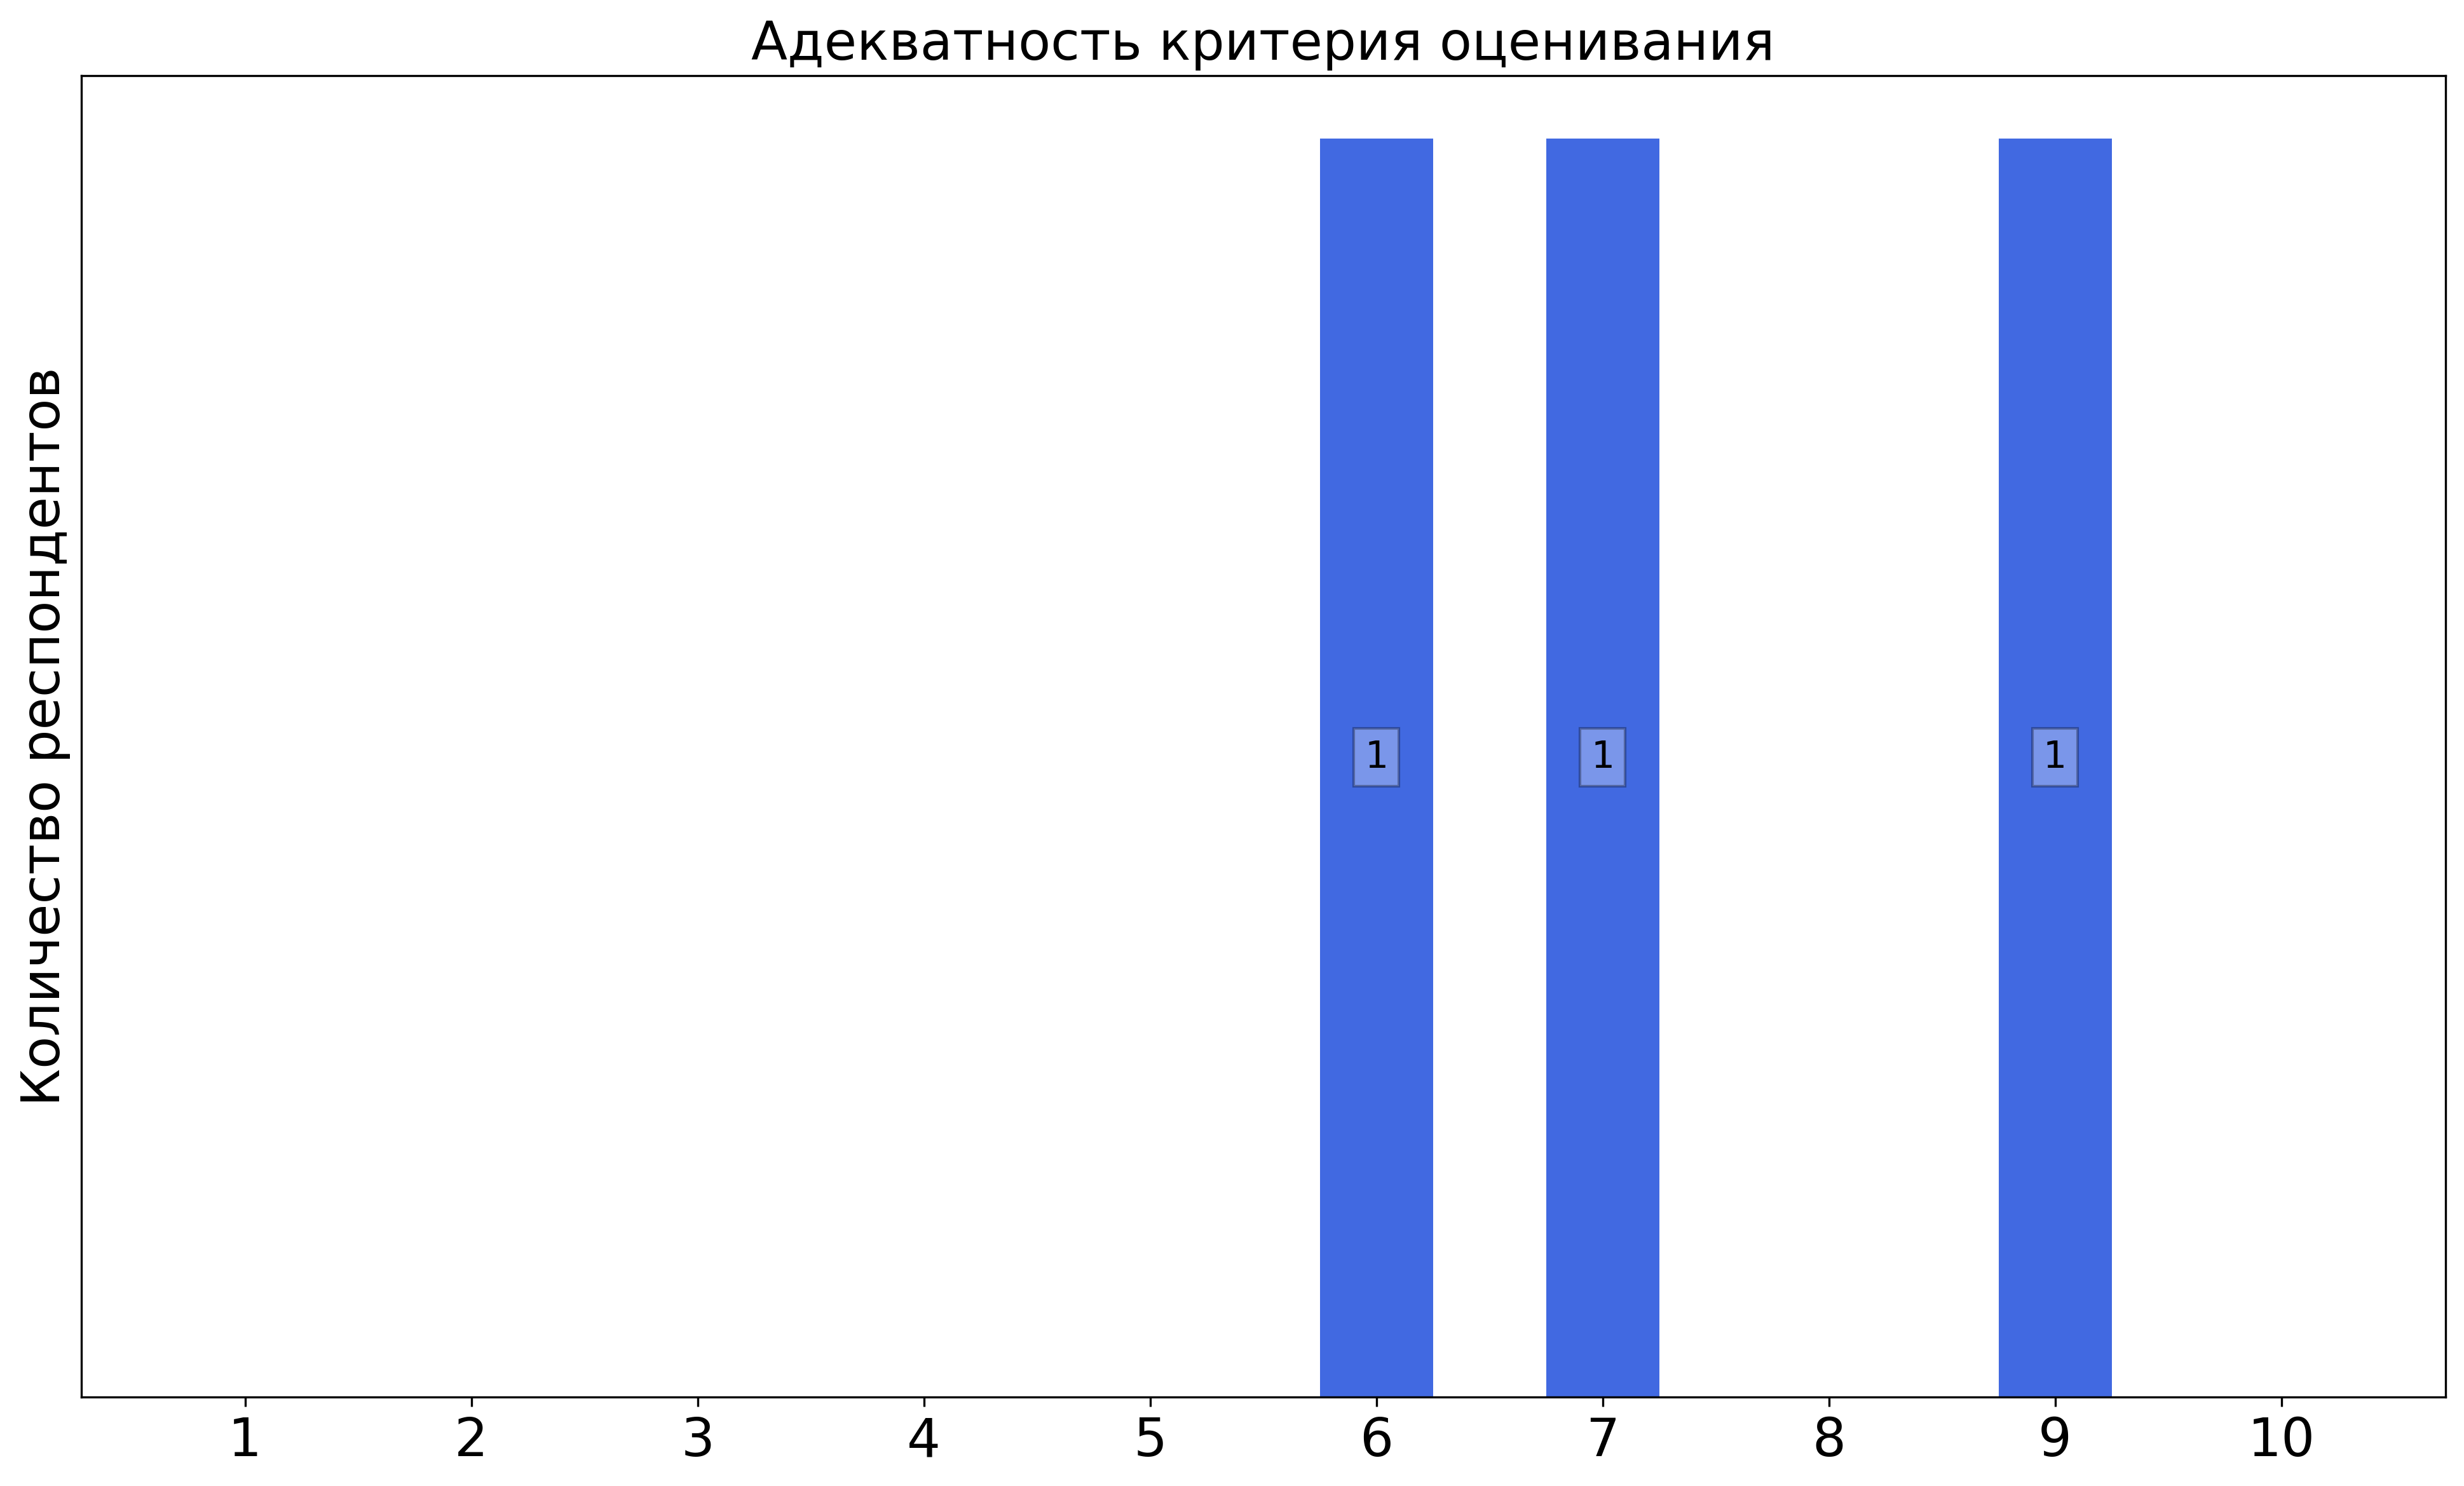
\includegraphics[width=\textwidth]{images/1 course/Общая физика - механика/labniks-marks-Веревочкин Ю.Г.-1.png}
            \end{subfigure}
            \begin{subfigure}[b]{0.45\textwidth}
                \centering
                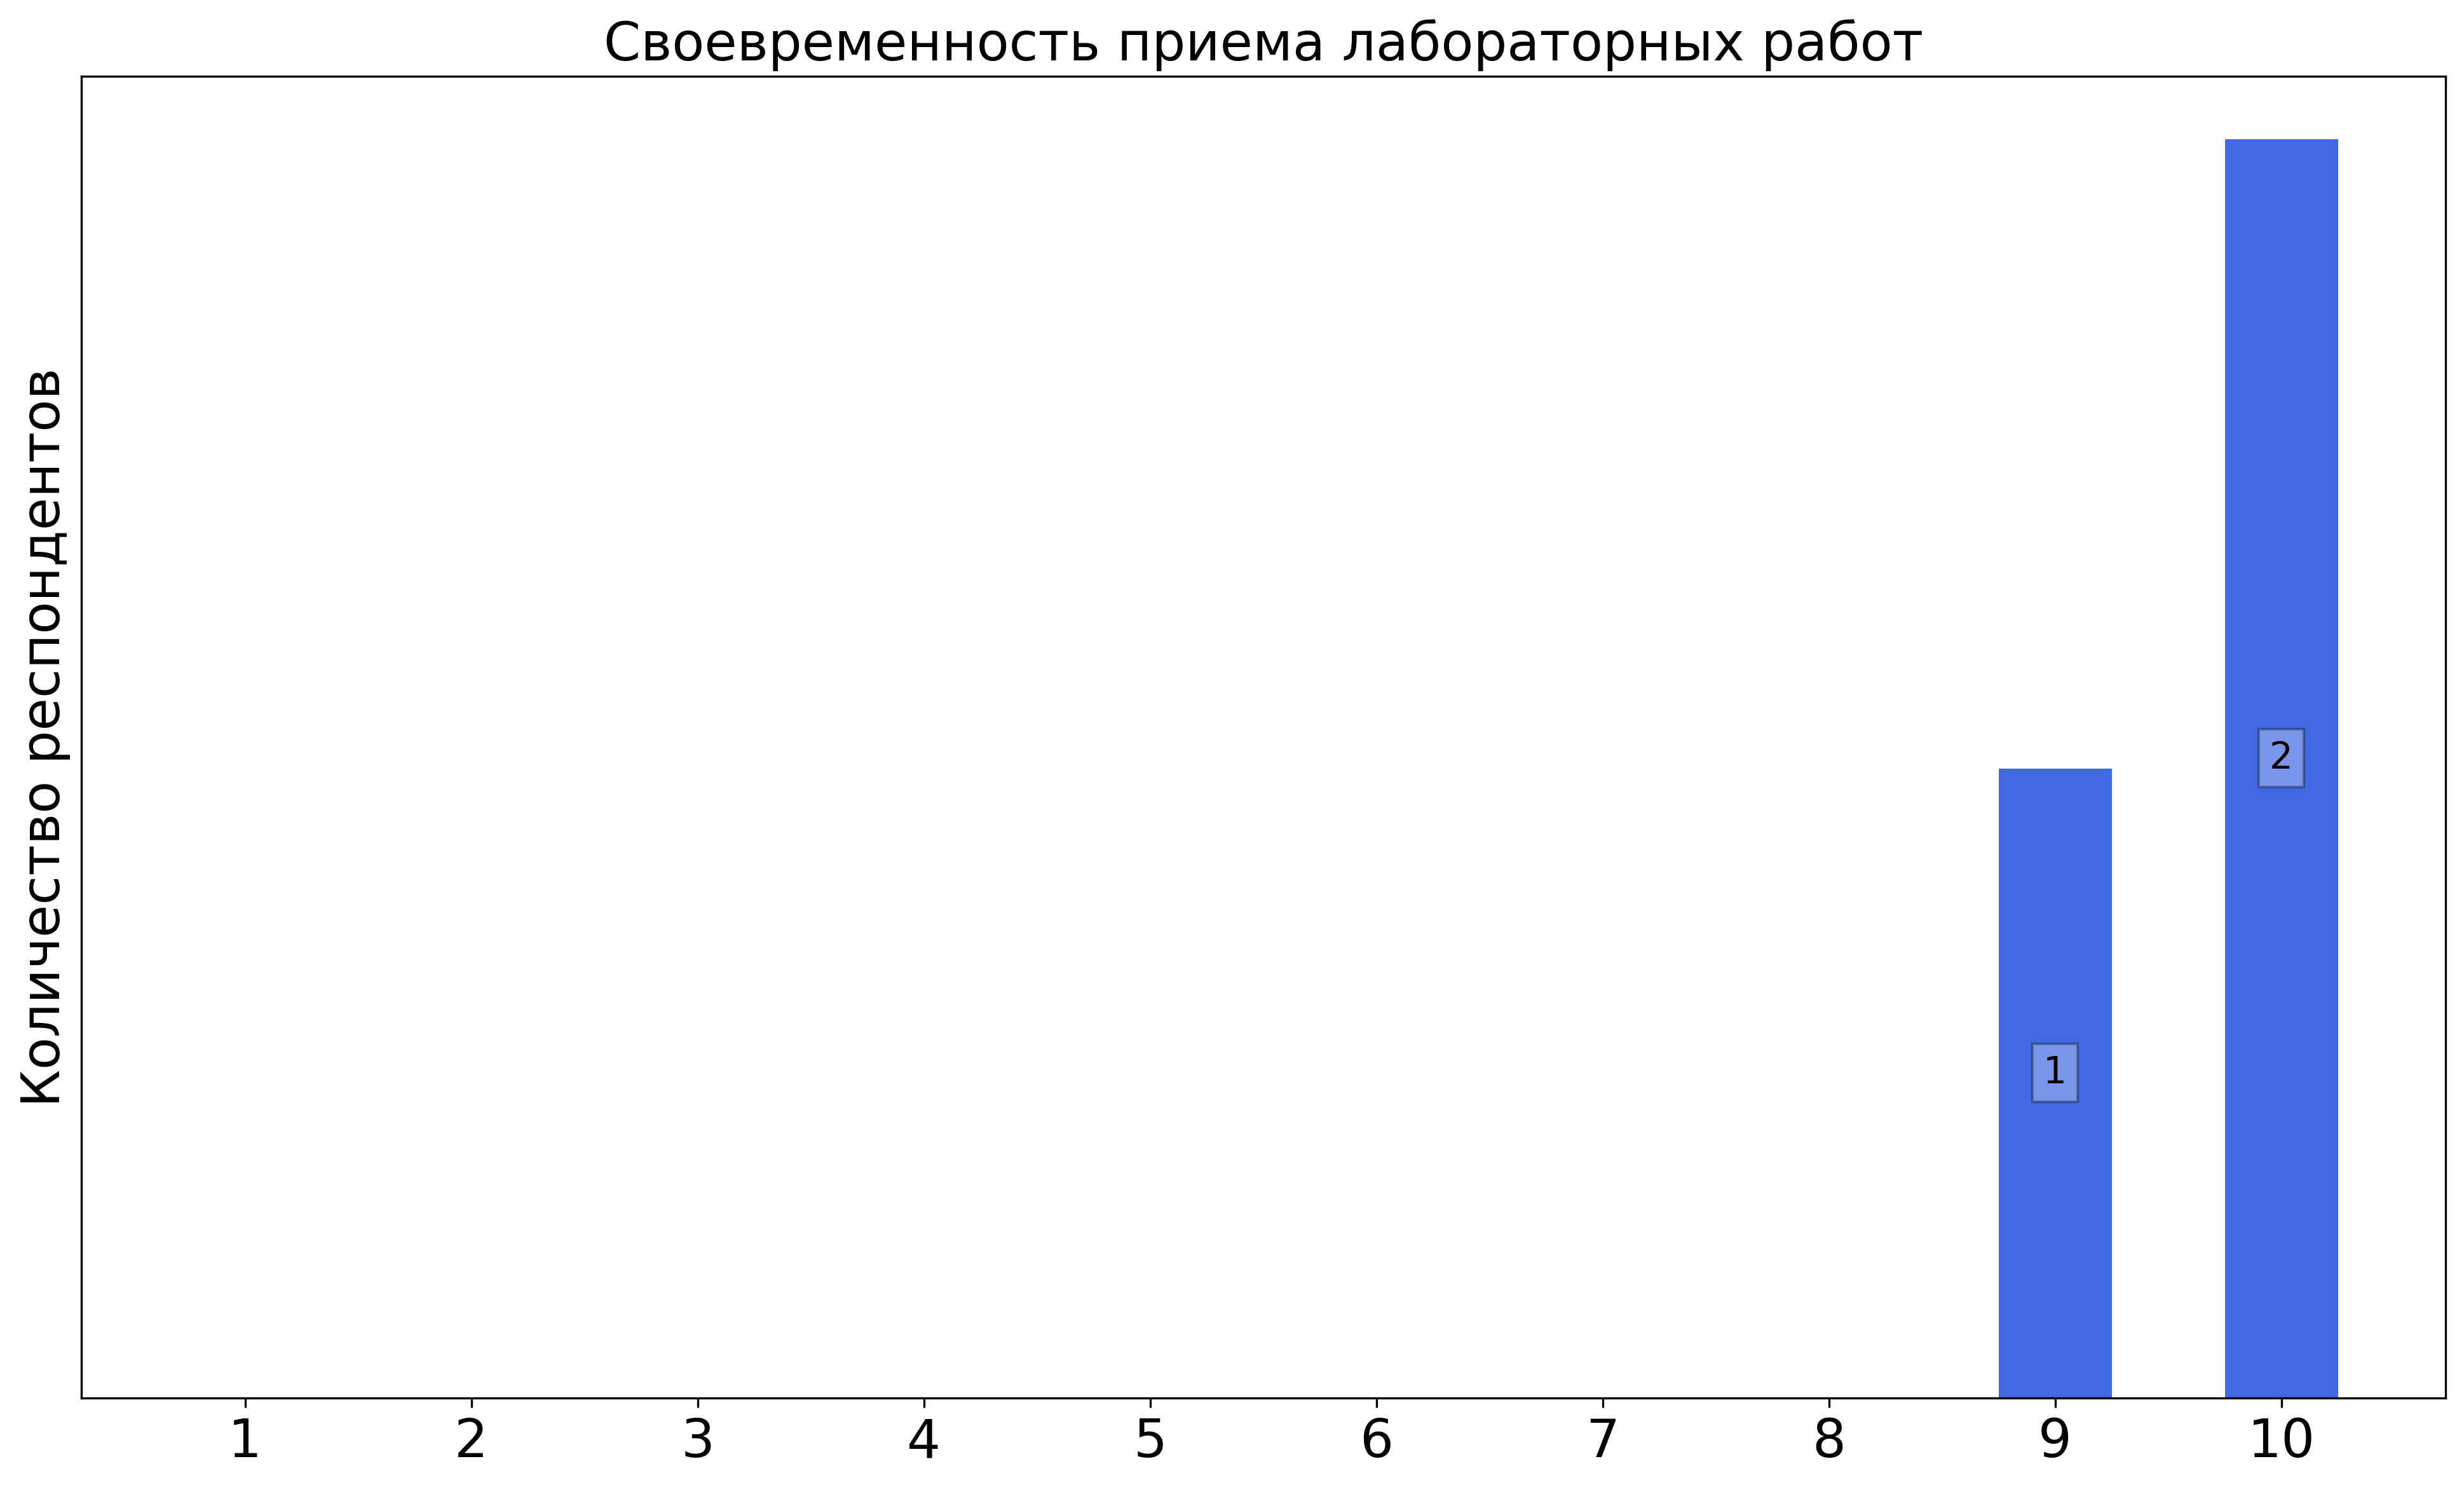
\includegraphics[width=\textwidth]{images/1 course/Общая физика - механика/labniks-marks-Веревочкин Ю.Г.-2.png}
            \end{subfigure}
            \begin{subfigure}[b]{0.45\textwidth}
                \centering
                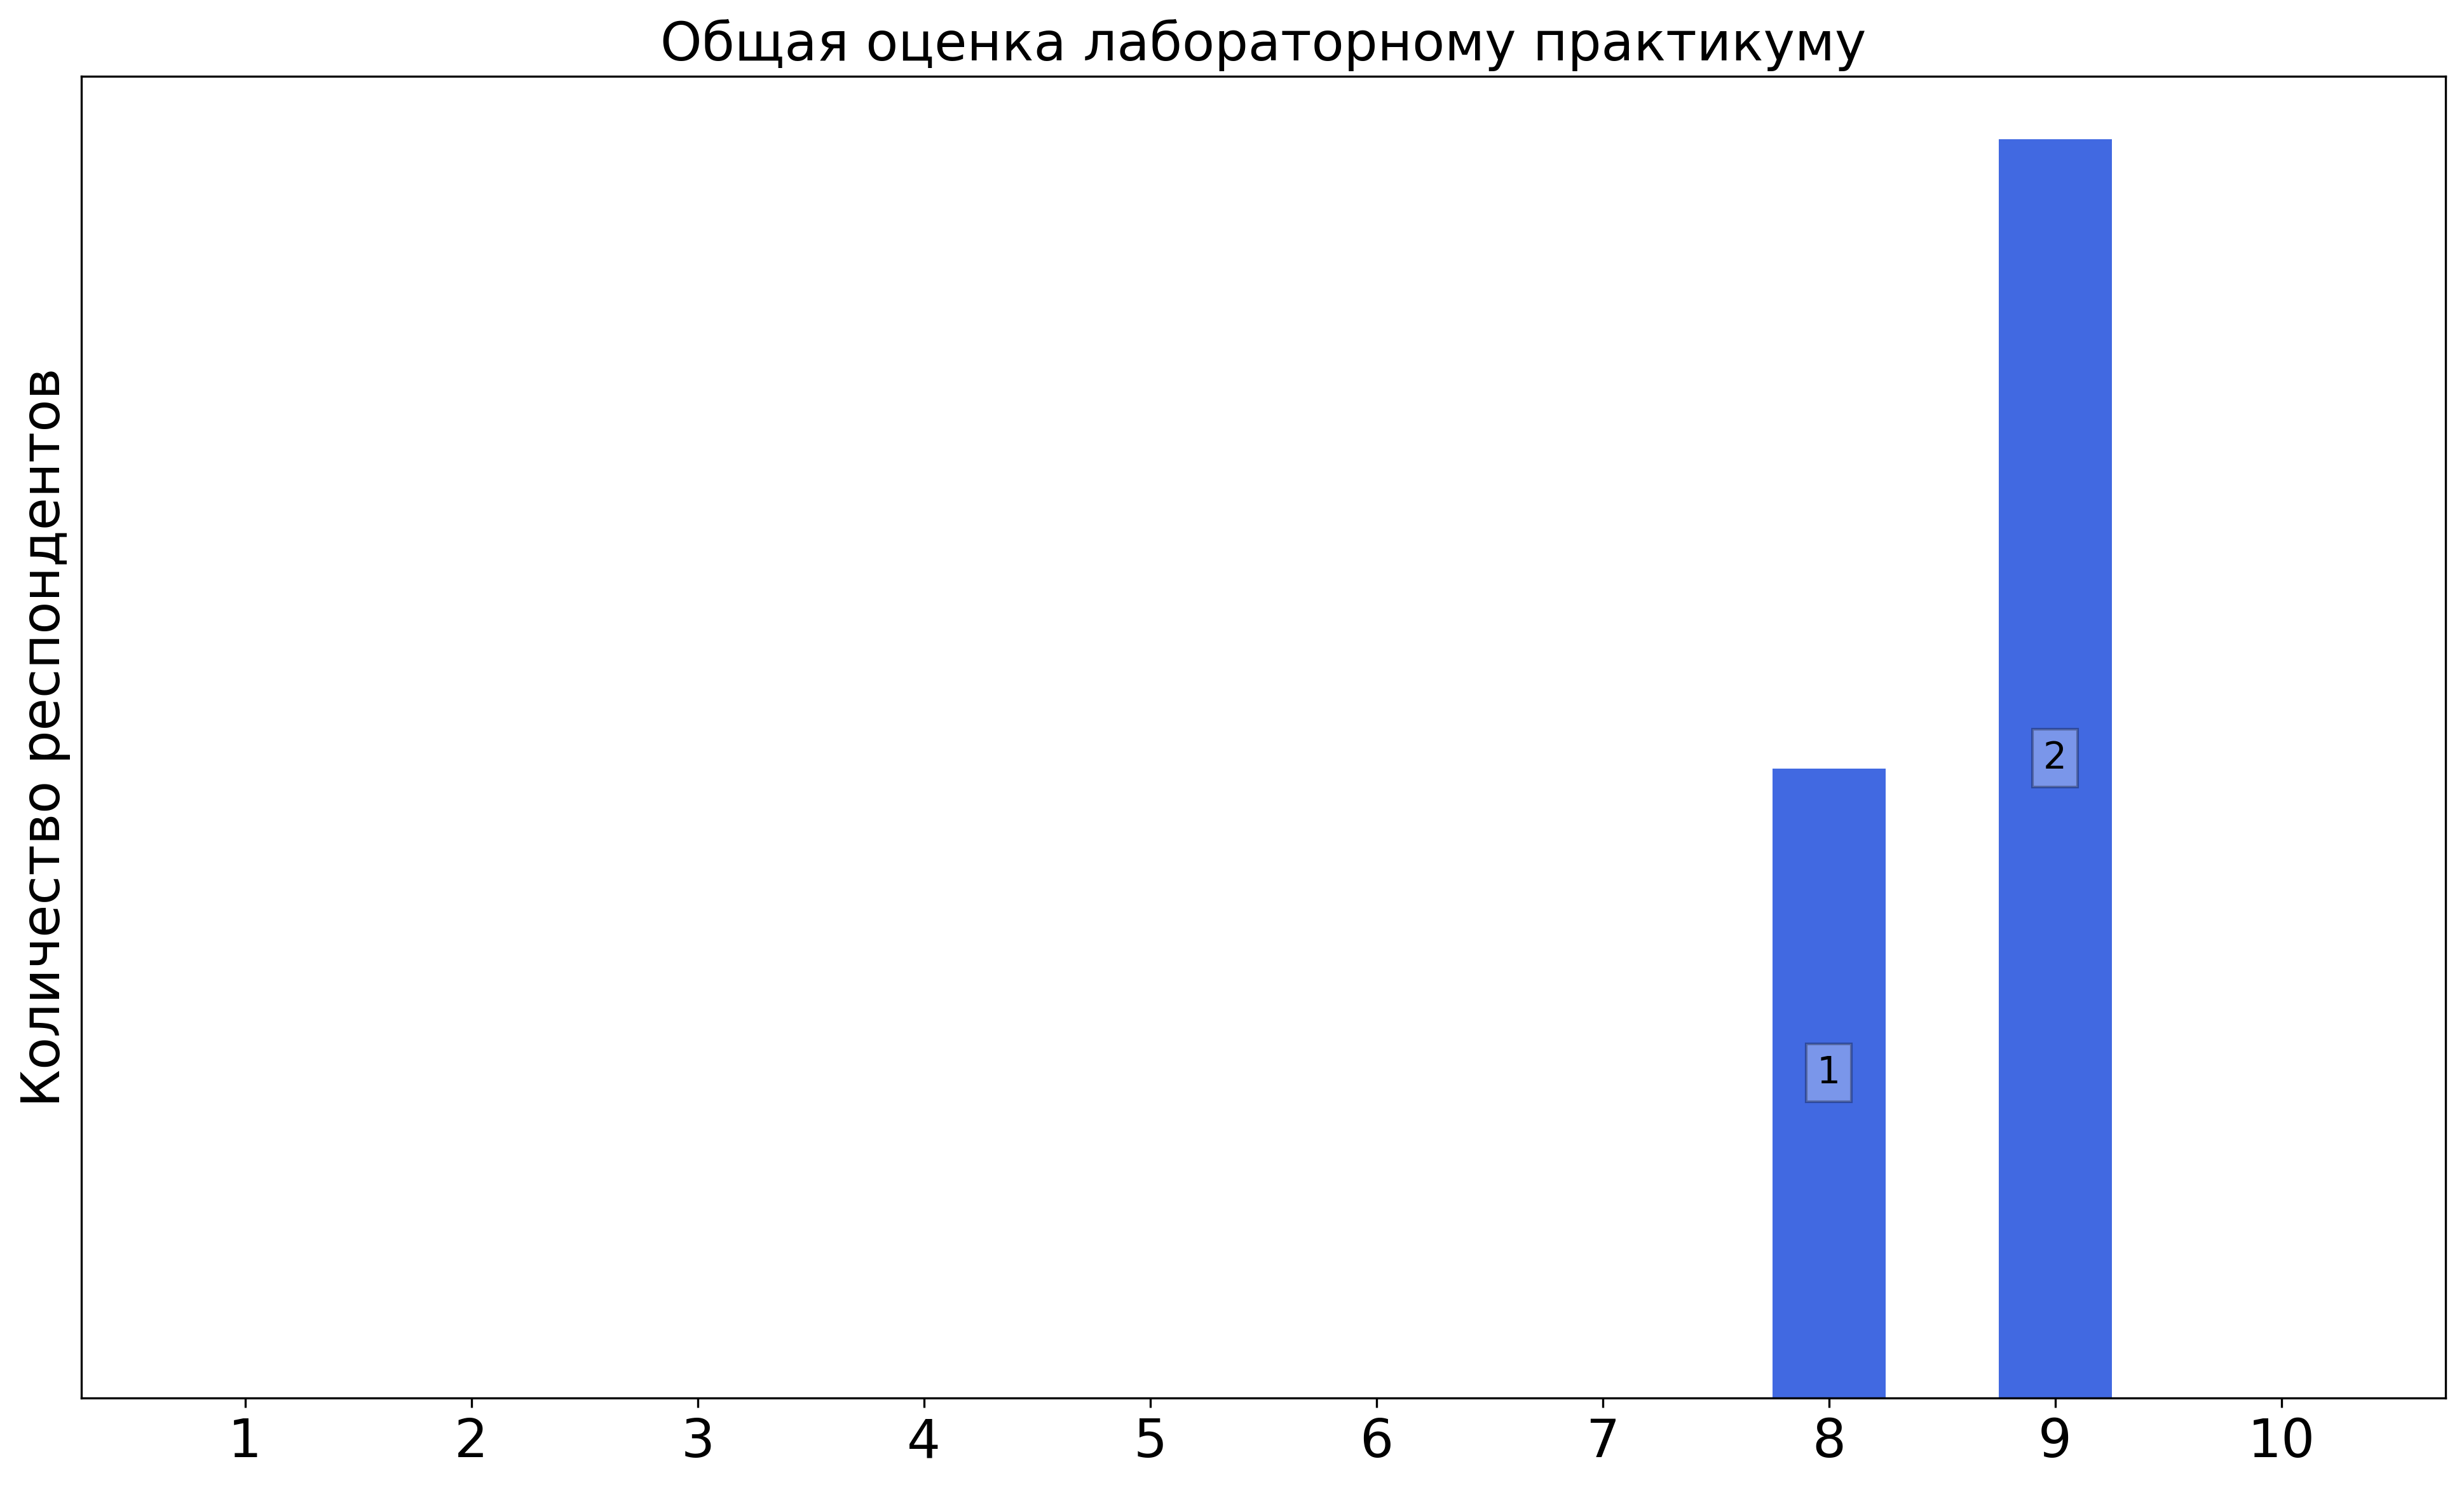
\includegraphics[width=\textwidth]{images/1 course/Общая физика - механика/labniks-marks-Веревочкин Ю.Г.-3.png}
            \end{subfigure}	
            \caption{Оценки респондентов о качестве преподавания лабораторных работ}
        \end{figure}


    \subsubsection{Отзыв студентов о лабораторных работах. Преподаватель: Джанибекова С.Х.}
		\begin{figure}[H]
			\centering
			\begin{subfigure}[b]{0.45\textwidth}
				\centering
				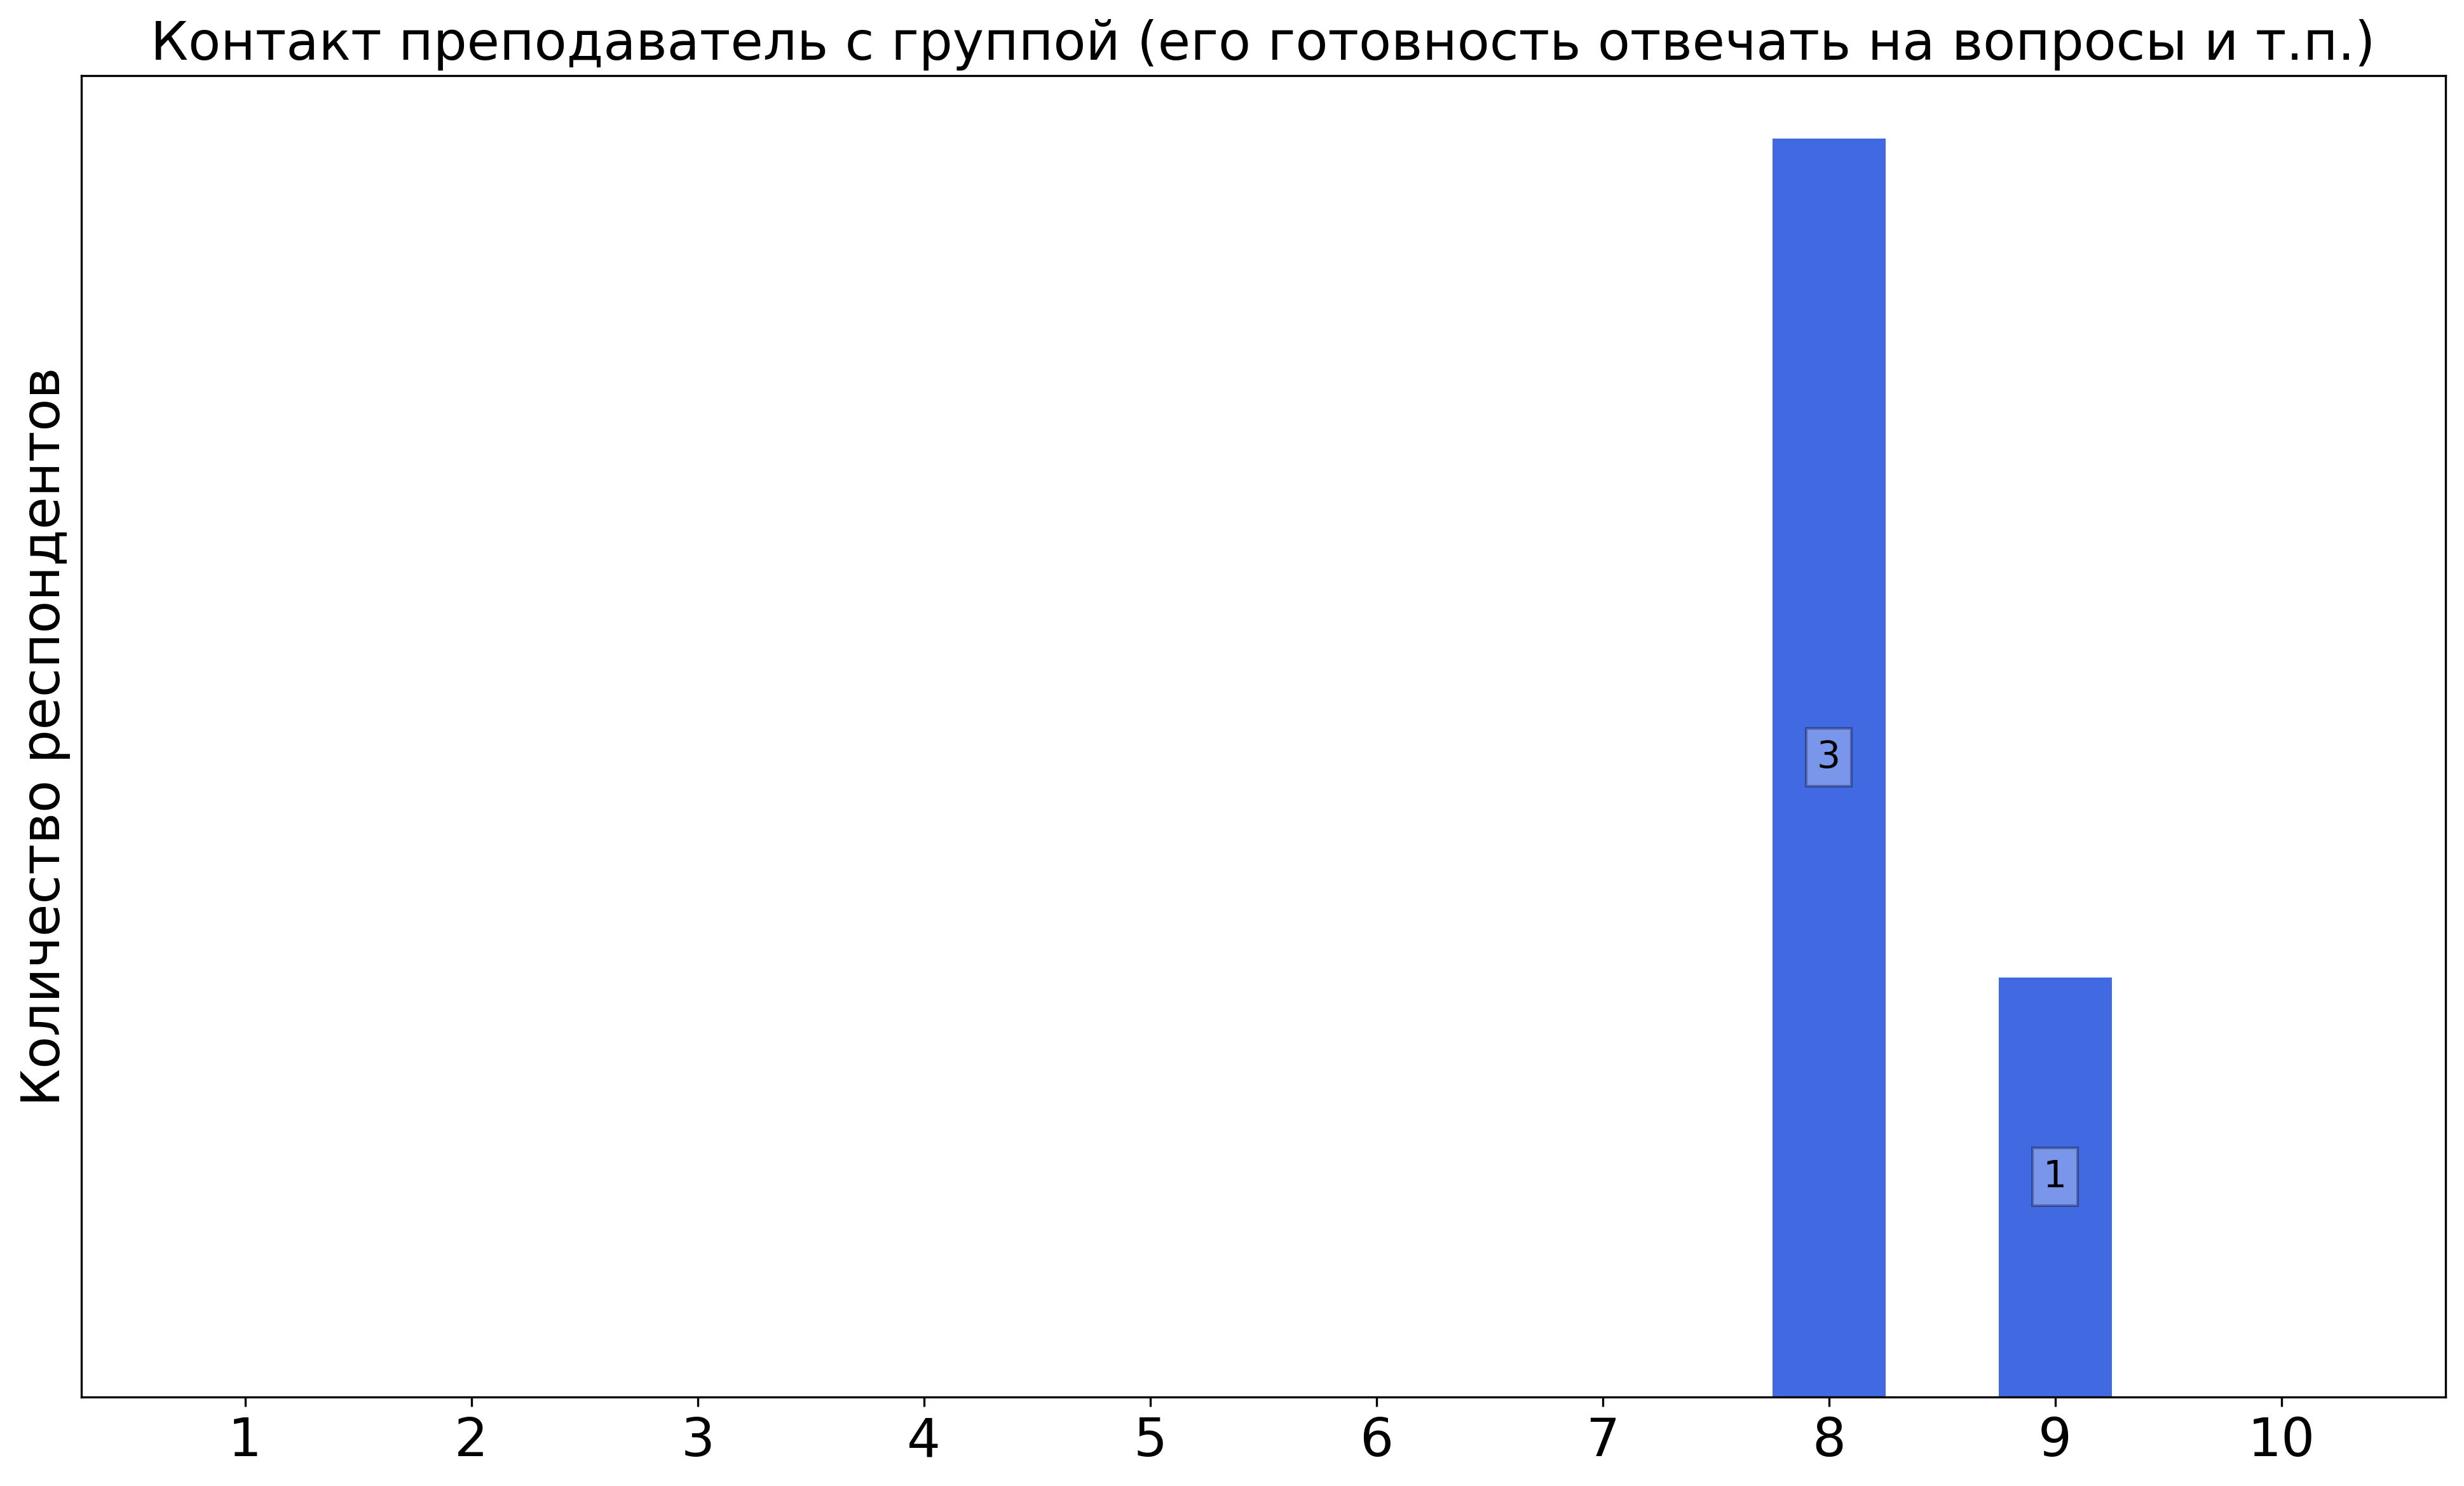
\includegraphics[width=\textwidth]{images/1 course/Общая физика - механика/labniks-marks-Джанибекова С.Х.-0.png}
			\end{subfigure}
			\begin{subfigure}[b]{0.45\textwidth}
				\centering
				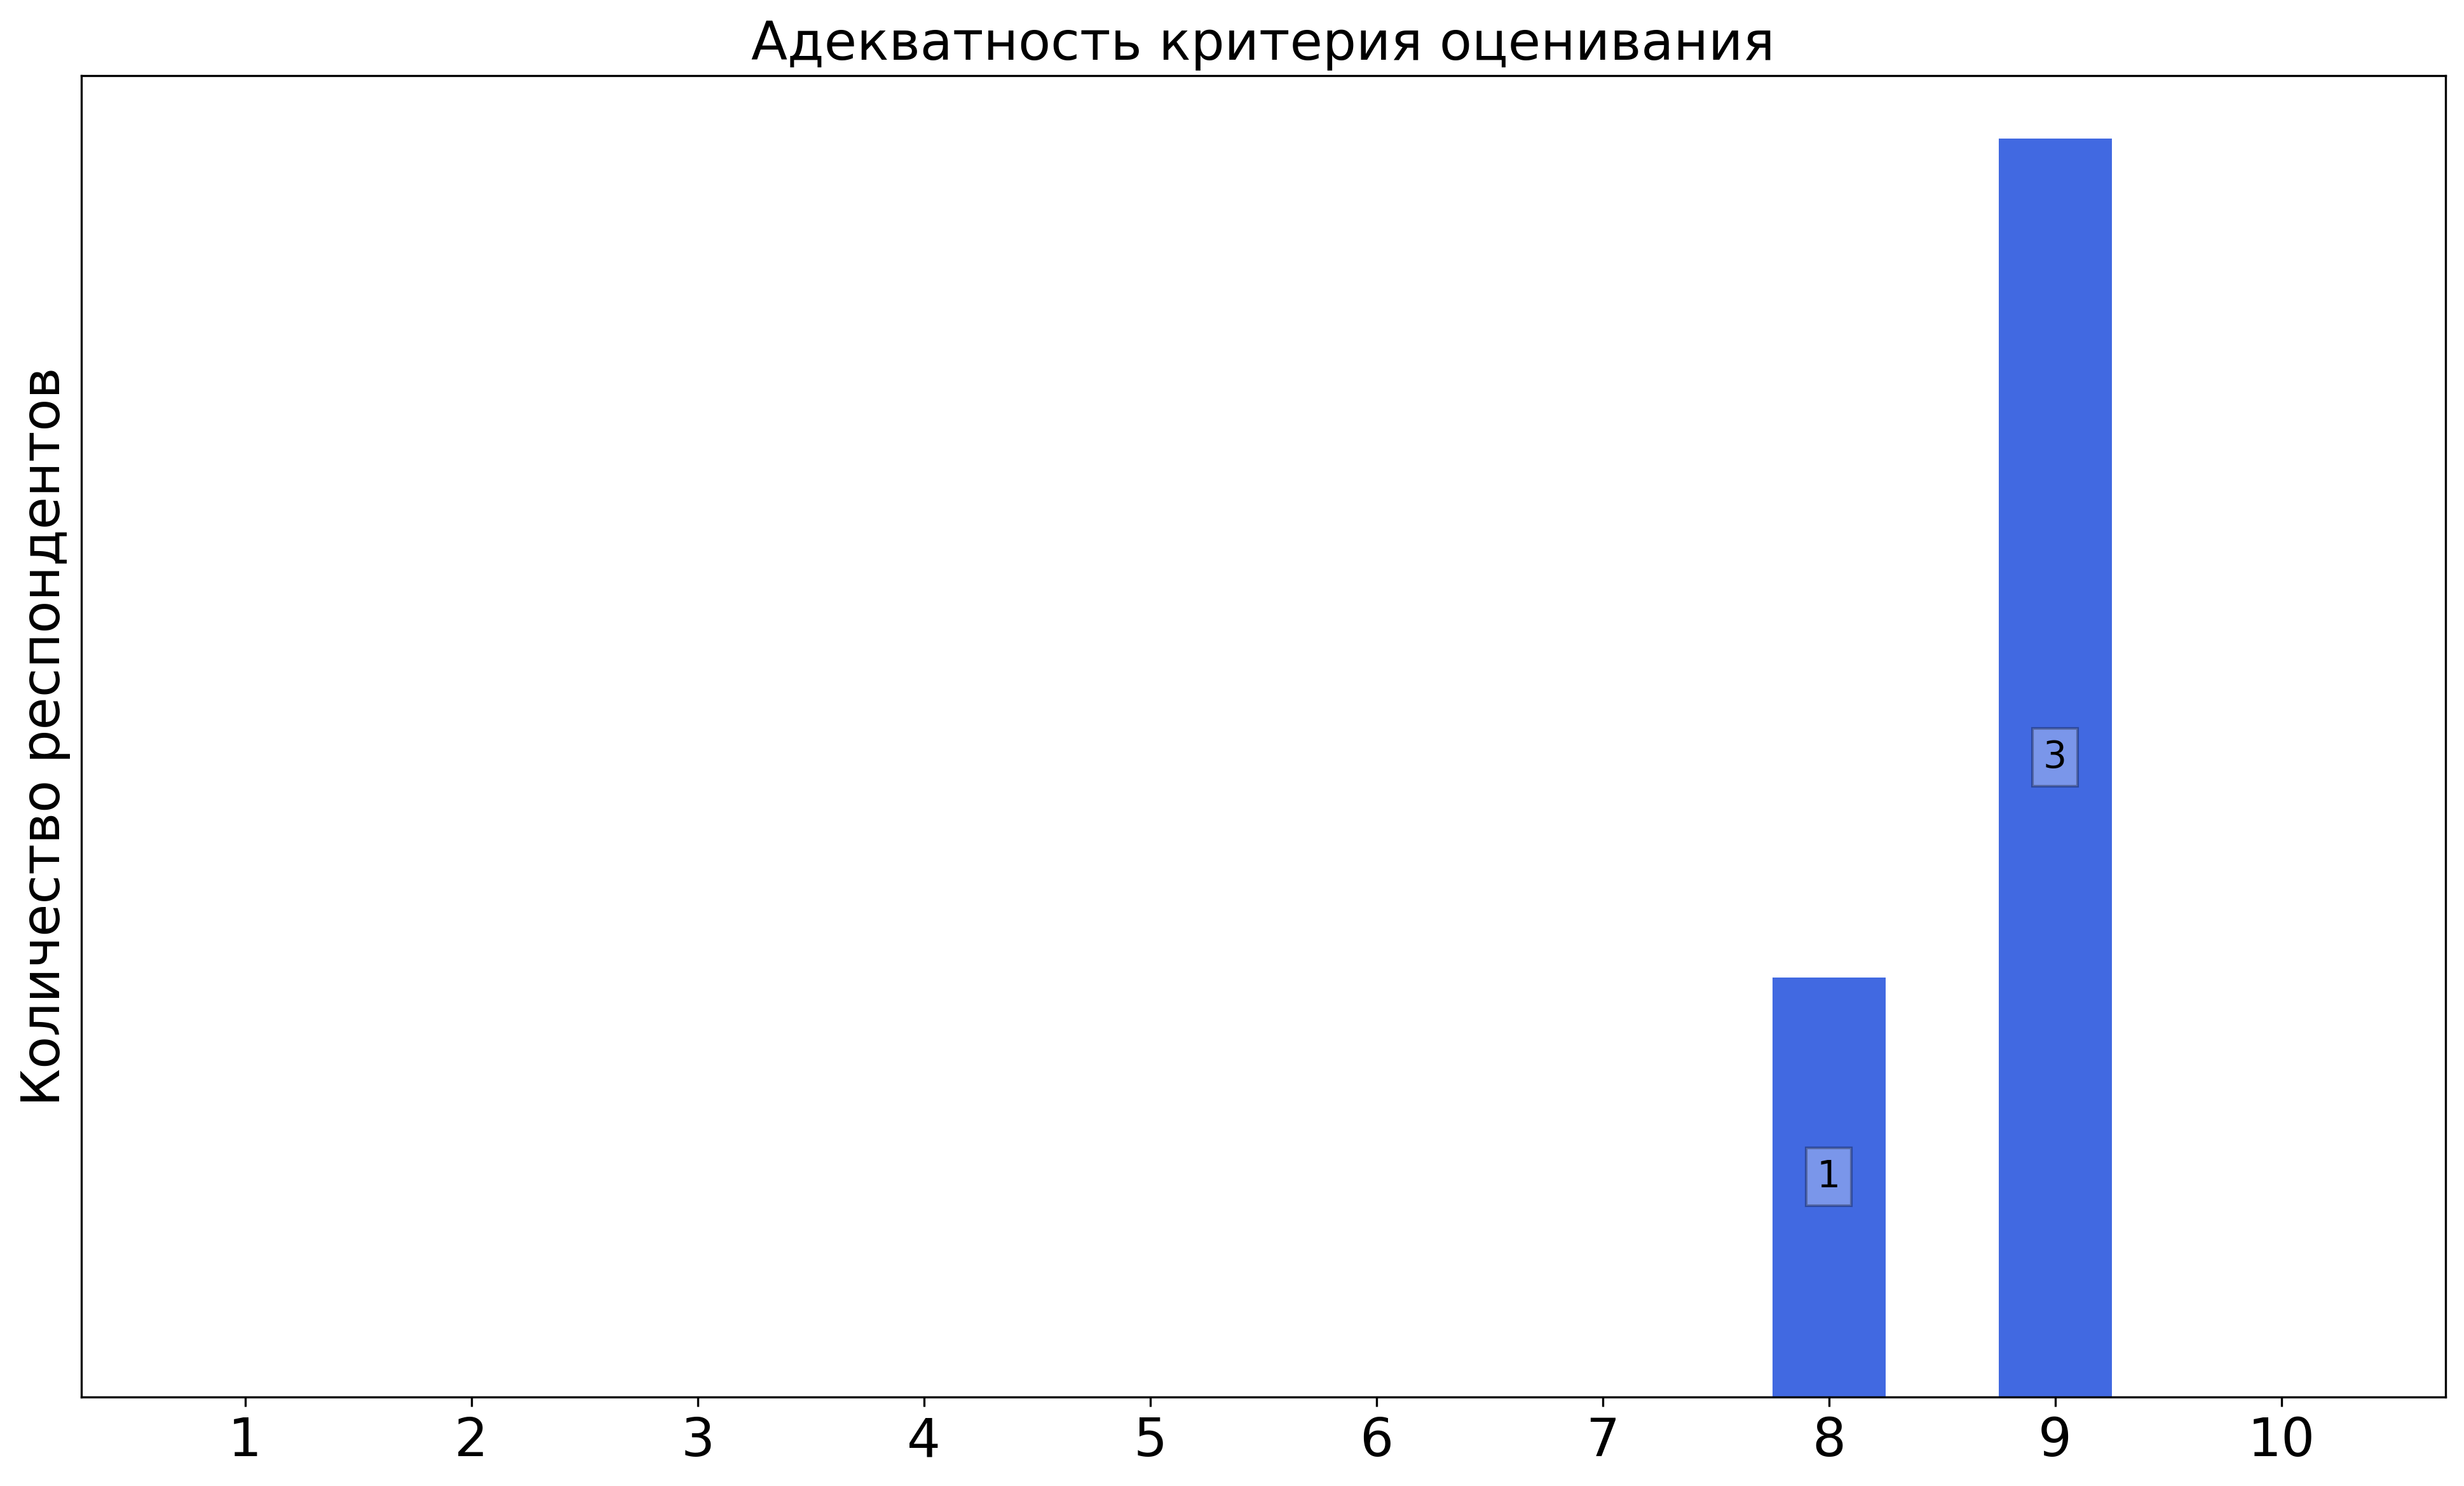
\includegraphics[width=\textwidth]{images/1 course/Общая физика - механика/labniks-marks-Джанибекова С.Х.-1.png}
			\end{subfigure}
			\begin{subfigure}[b]{0.45\textwidth}
				\centering
				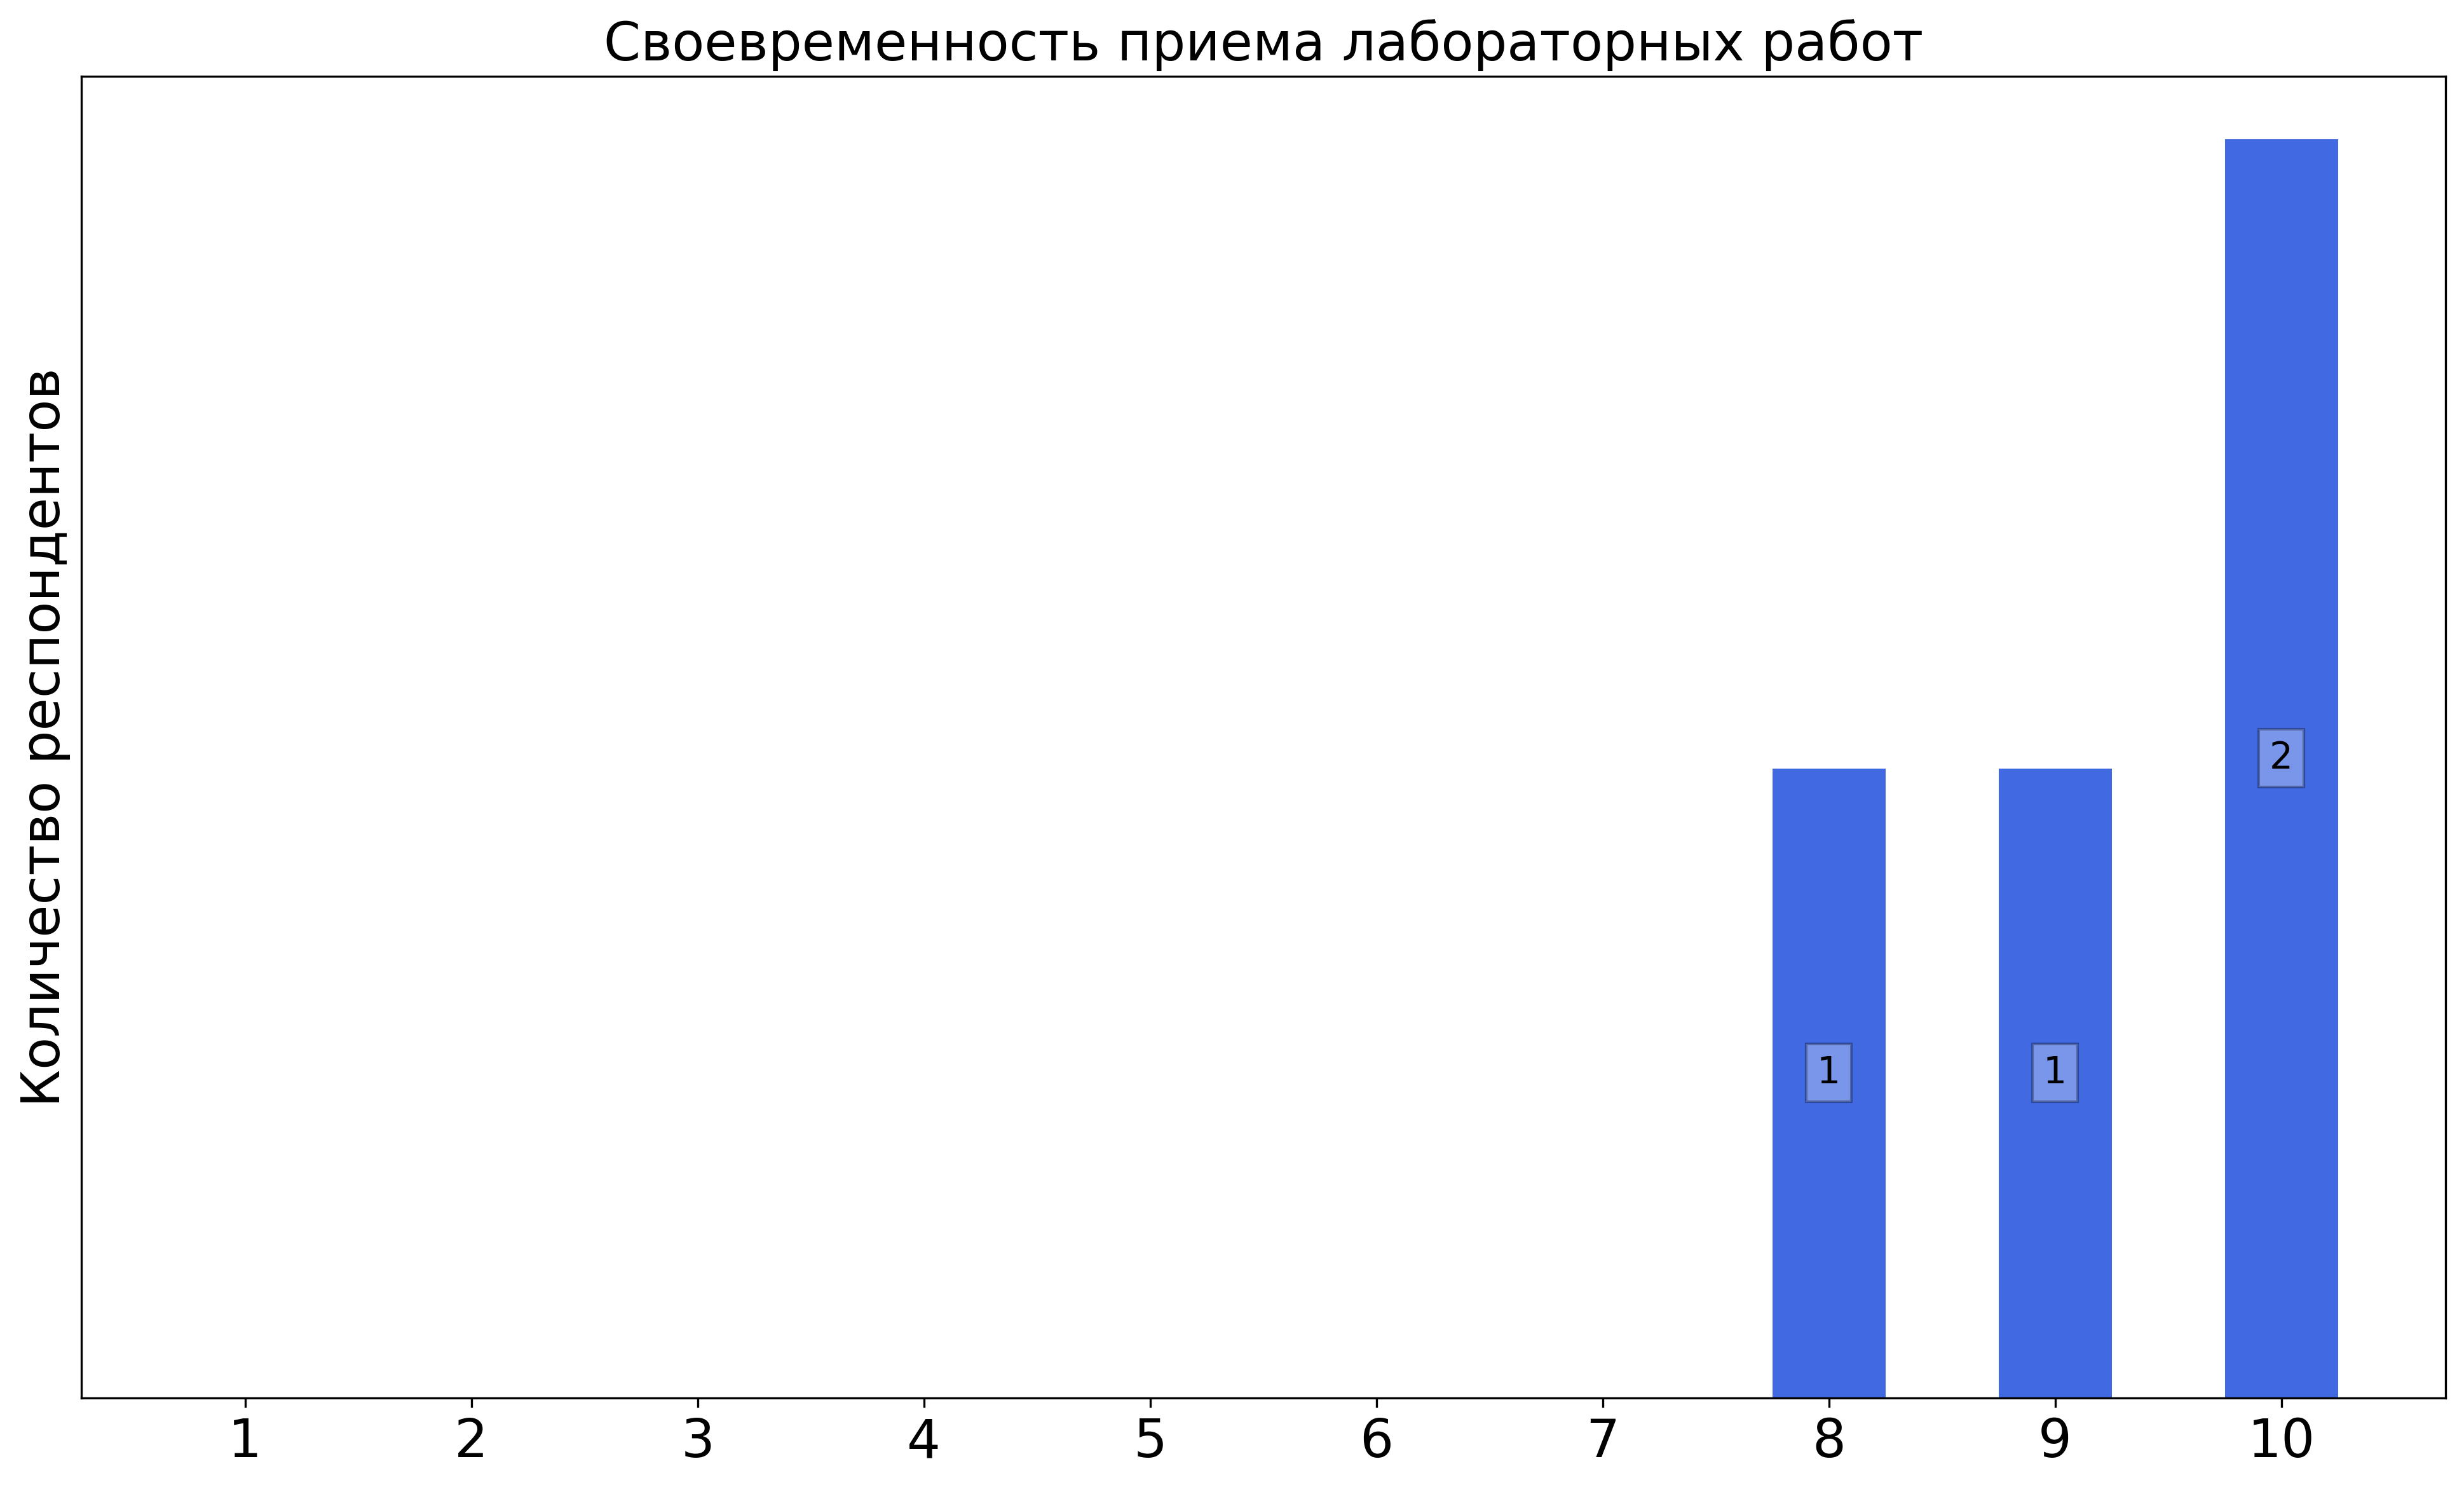
\includegraphics[width=\textwidth]{images/1 course/Общая физика - механика/labniks-marks-Джанибекова С.Х.-2.png}
			\end{subfigure}
			\begin{subfigure}[b]{0.45\textwidth}
				\centering
				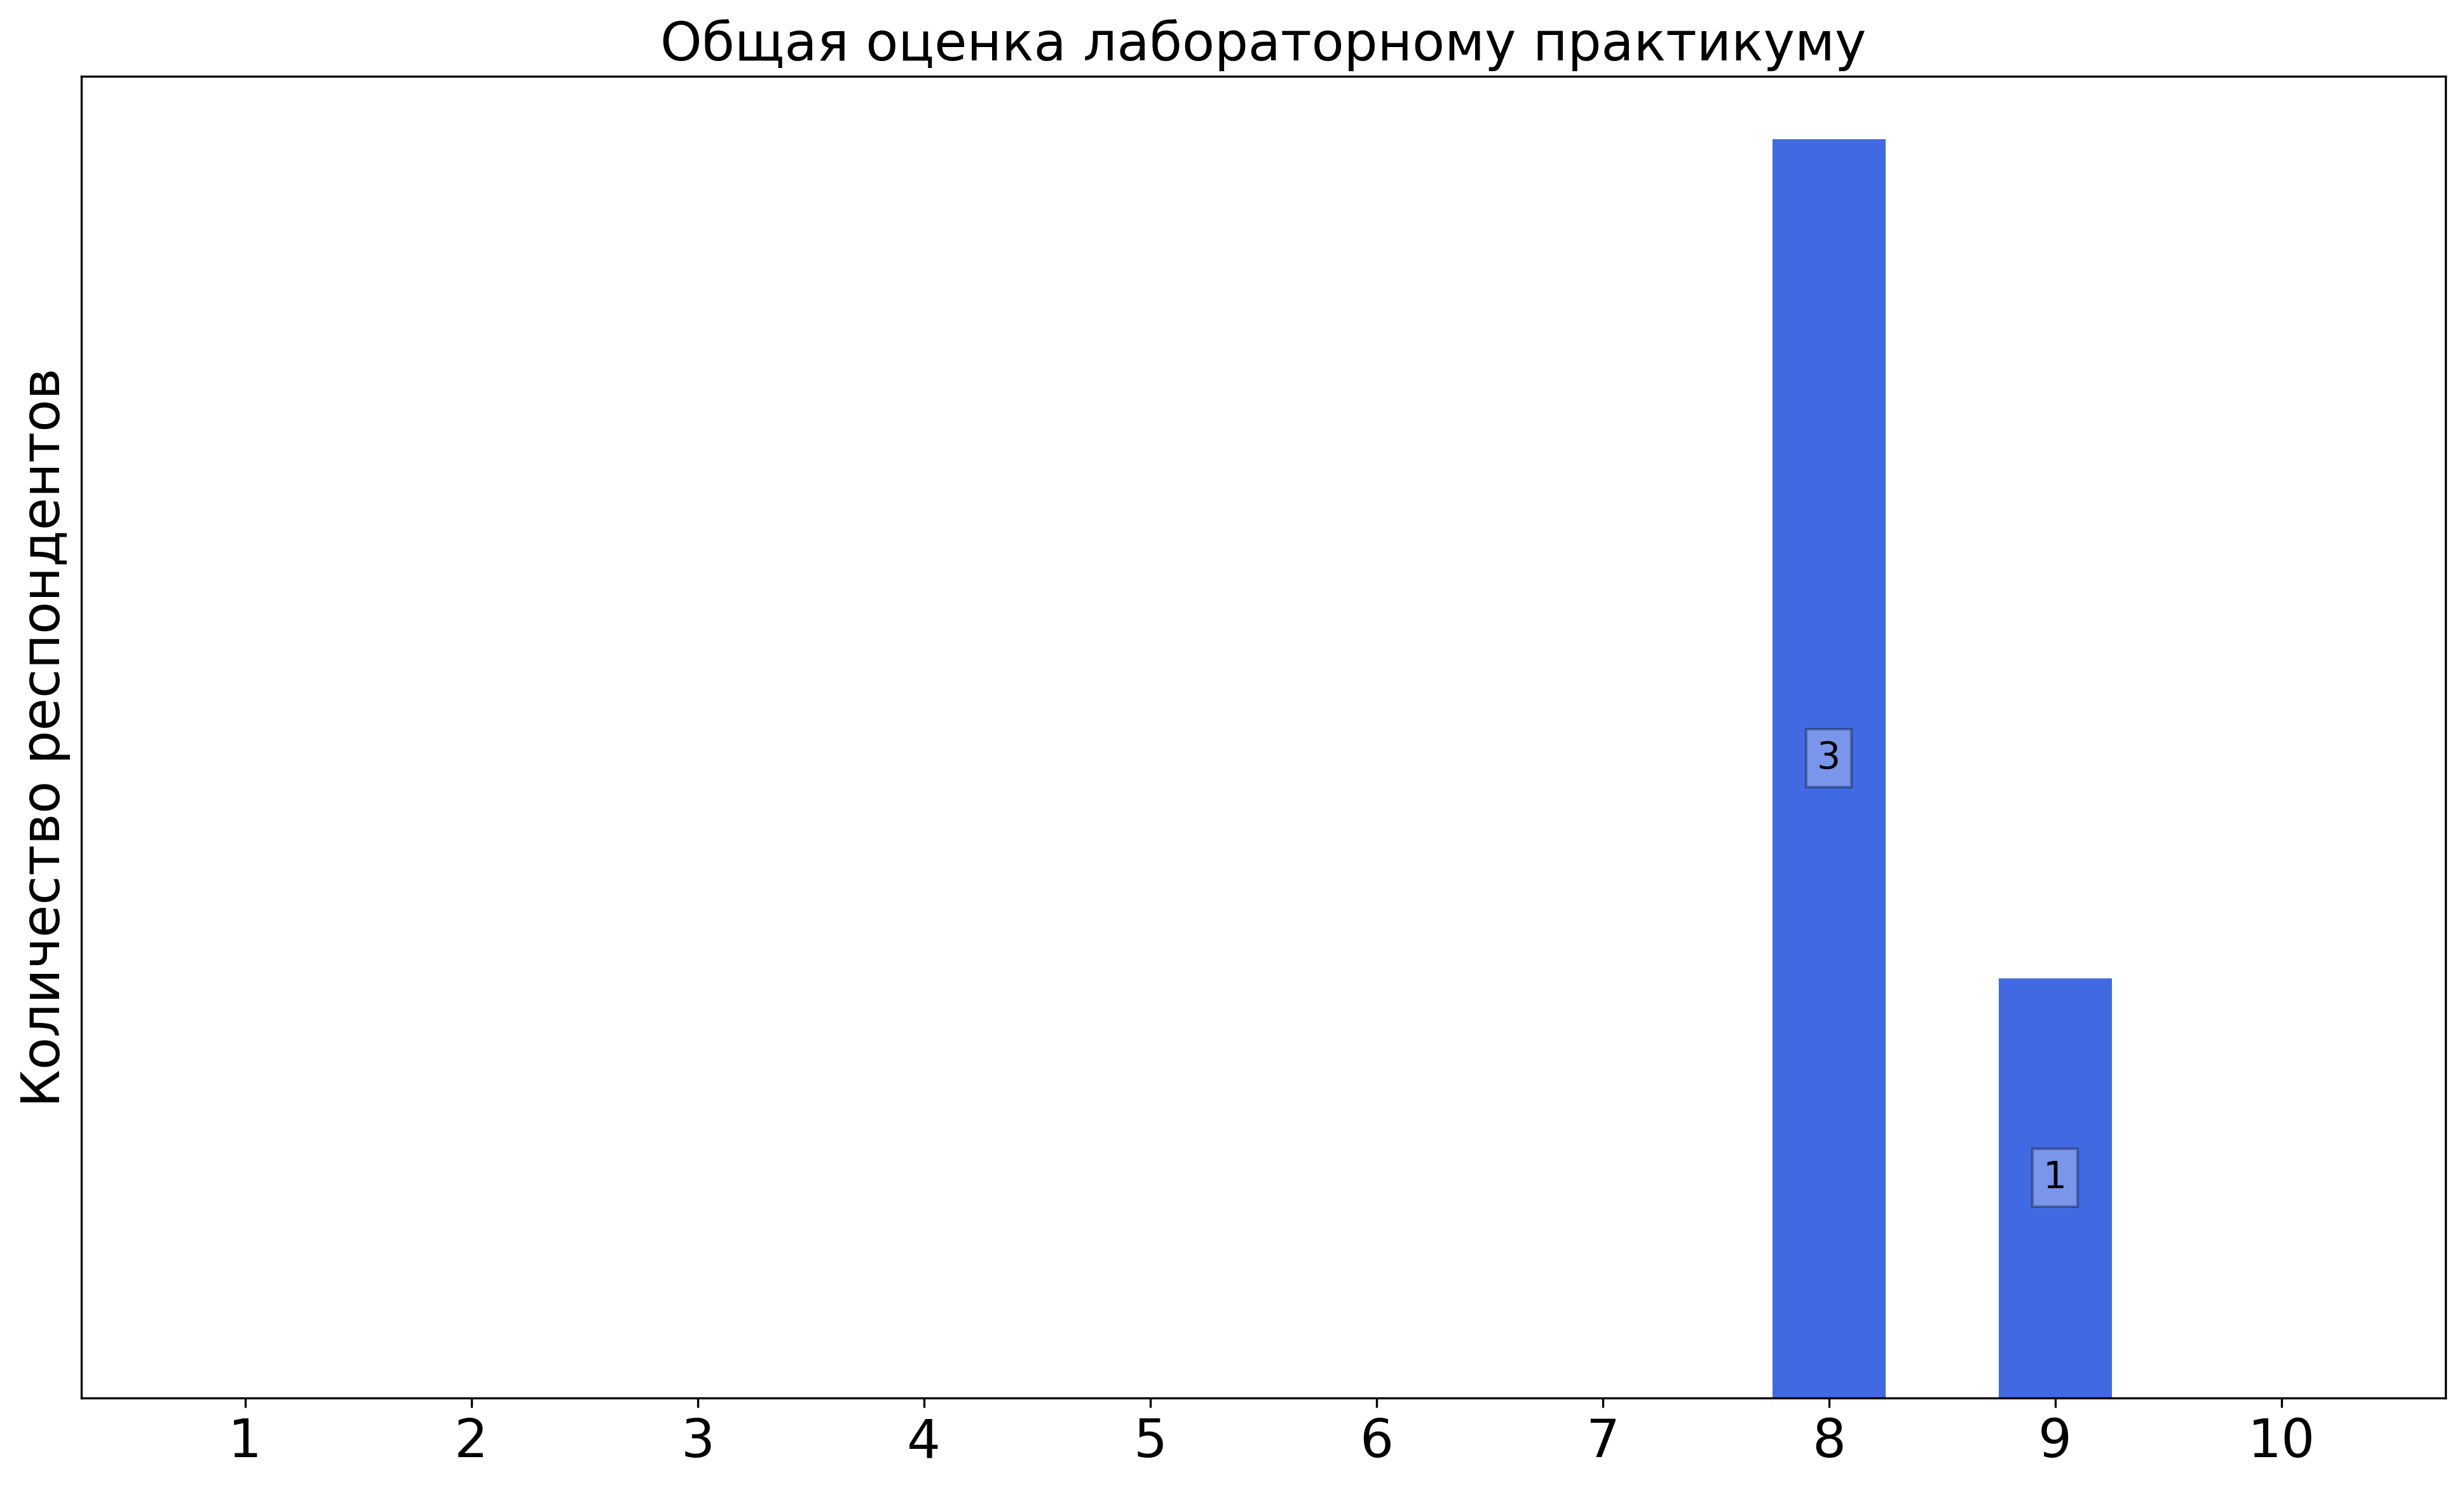
\includegraphics[width=\textwidth]{images/1 course/Общая физика - механика/labniks-marks-Джанибекова С.Х.-3.png}
			\end{subfigure}	
			\caption{Оценки респондентов о качестве преподавания лабораторных работ}
		\end{figure}

		\textbf{Комментарии студентов о преподавателе\protect\footnote{сохранены оригинальные орфография и пунктуация}}
            \begin{commentbox} 
                Отличный способ понять физику. Материал методичек понятный, интересный и хорошо усваивающийся. Большой плюс в том, что выполнять расчёты разрешалось в любой удобной программе, а основной упор делался именно на усвоение студентом теоретического и практического материала (студент пересказывает теорию и практику, а преподаватель в конце делает замечания и объясняет то, что студент не понял или сделал неправильно)
            \end{commentbox} 
       
            \begin{commentbox} 
                Лабы принимаются быстро, практически у всех было 8 либо 9. Но ощущения того, что  преподаватель действительно шарит, не было. Предмет достаточно интересный, однако времени на него нужно тратить немало. 
            \end{commentbox}
        
        
    \subsubsection{Отзыв студентов о лабораторных работах. Преподаватель: Долгих Е.А.}
        \begin{figure}[H]
            \centering
            \begin{subfigure}[b]{0.45\textwidth}
                \centering
                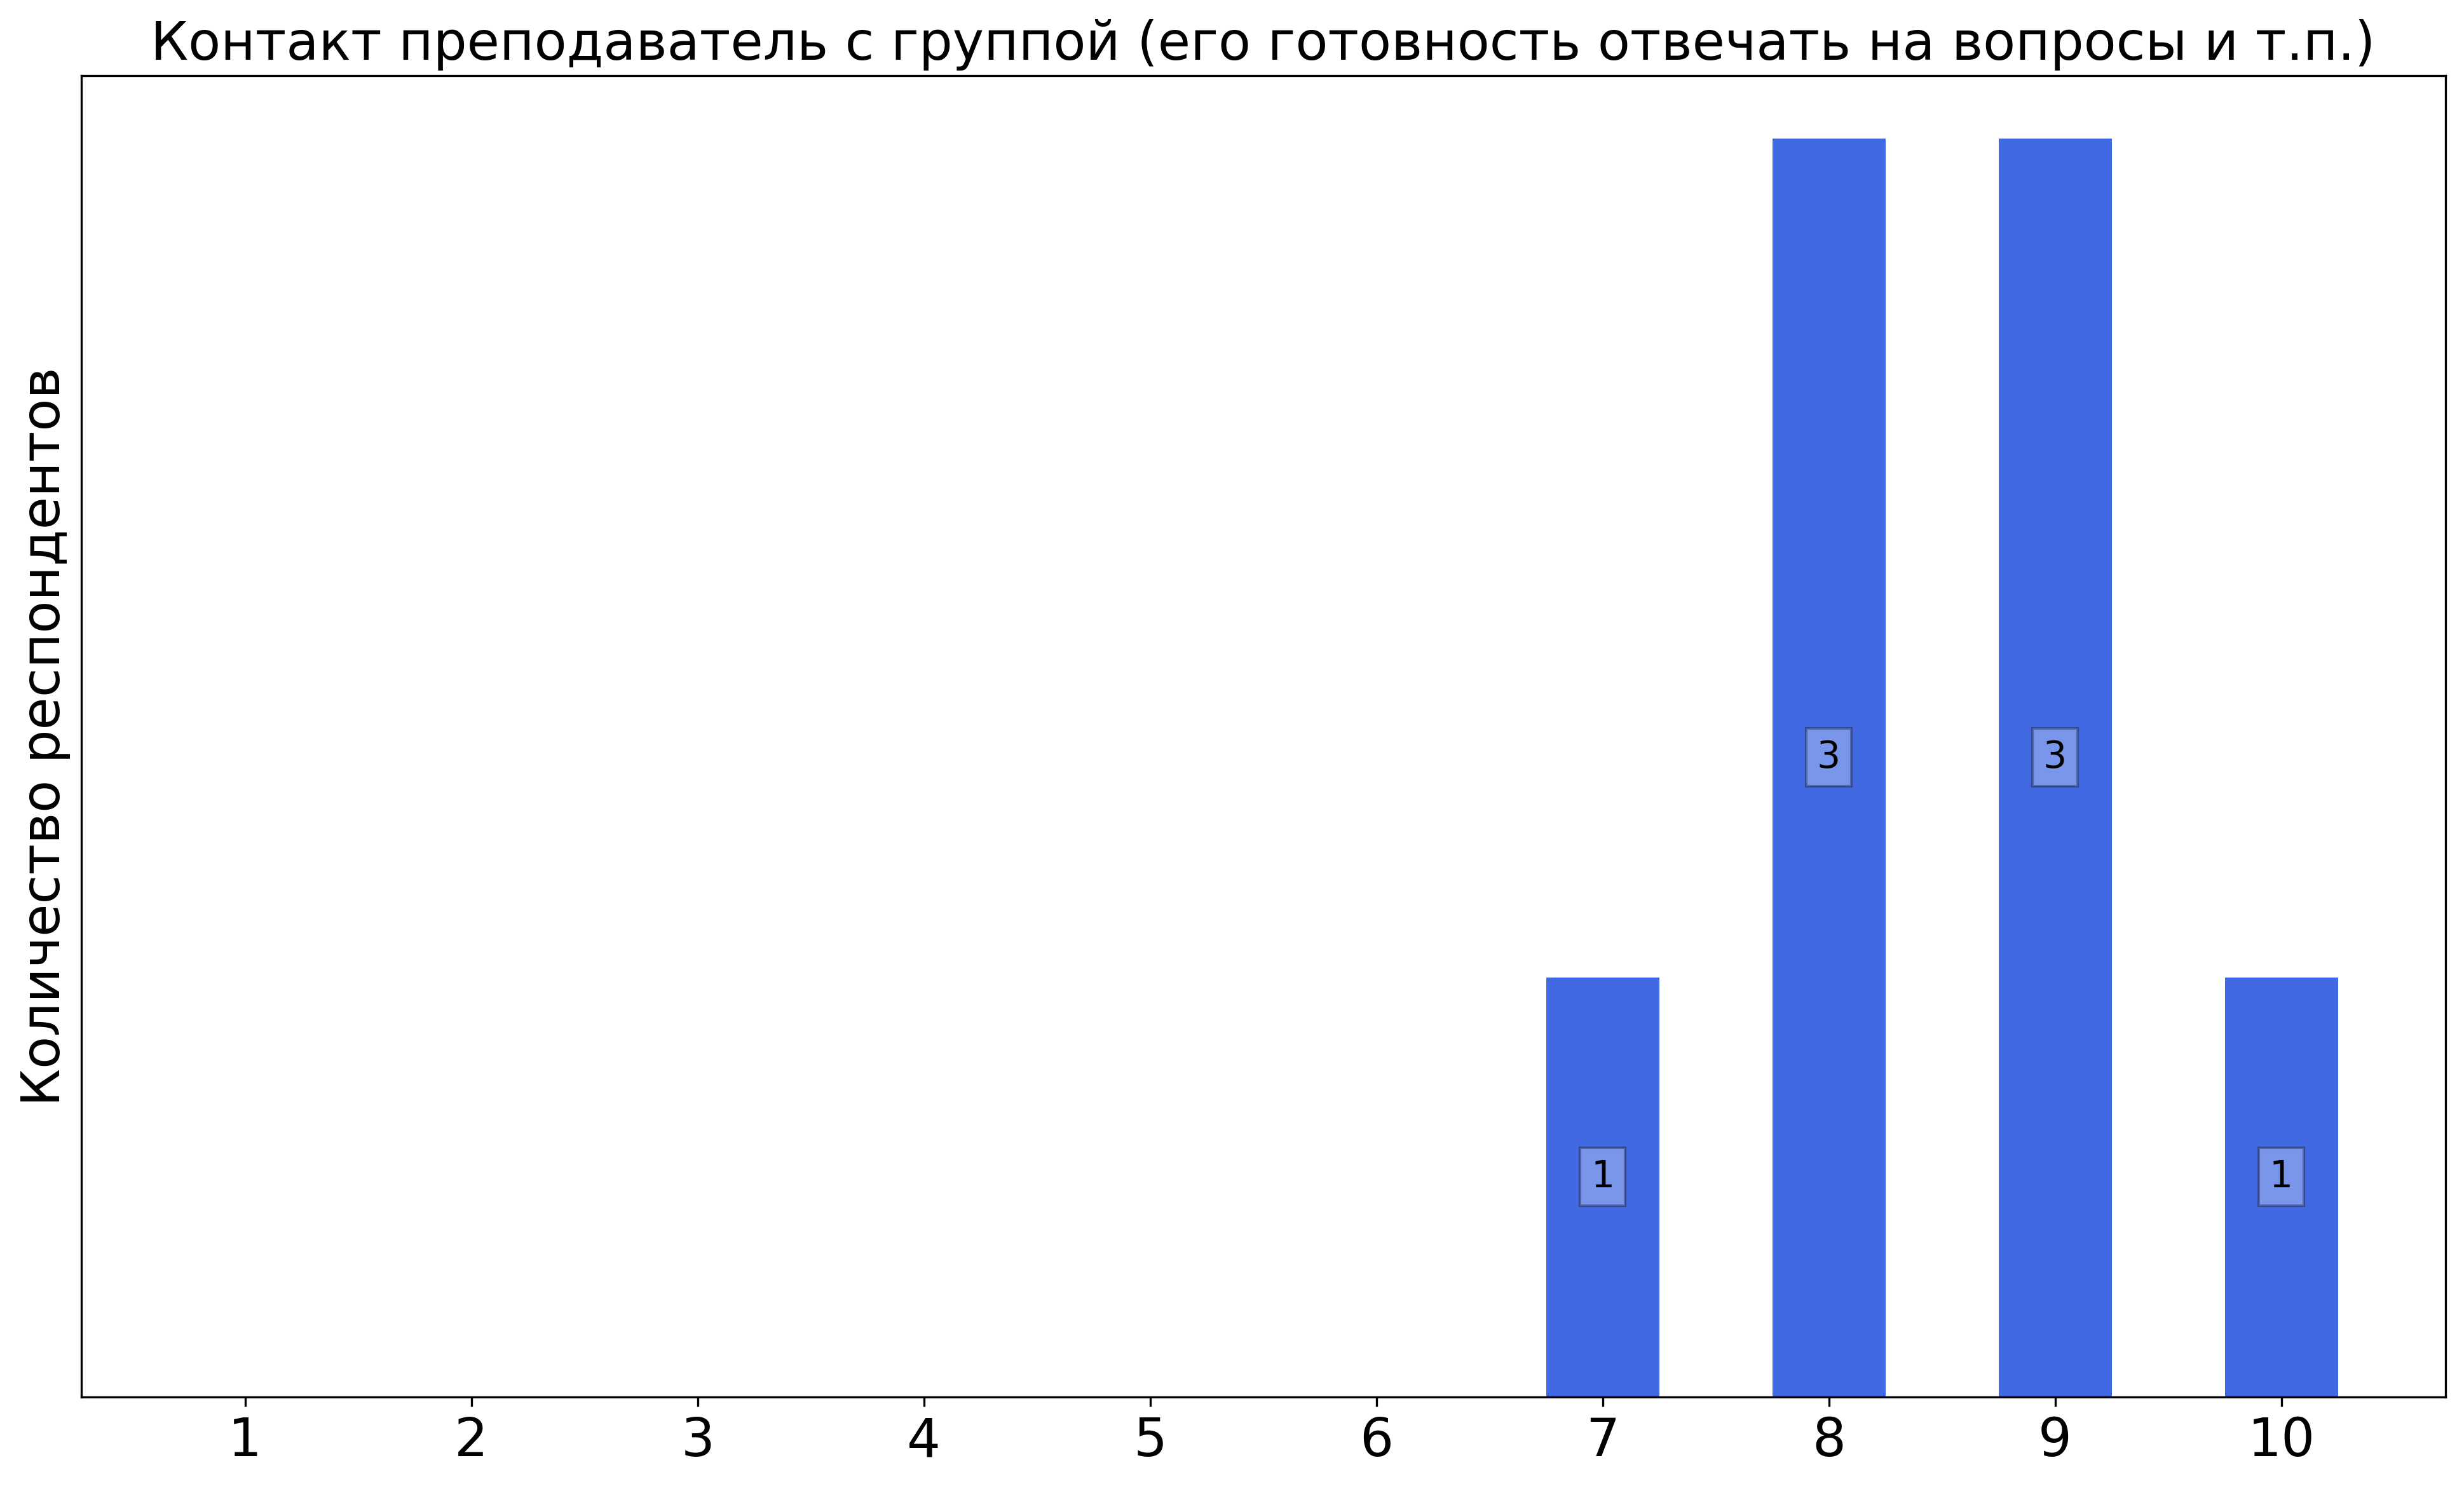
\includegraphics[width=\textwidth]{images/1 course/Общая физика - механика/labniks-marks-Долгих Е.А.-0.png}
            \end{subfigure}
            \begin{subfigure}[b]{0.45\textwidth}
                \centering
                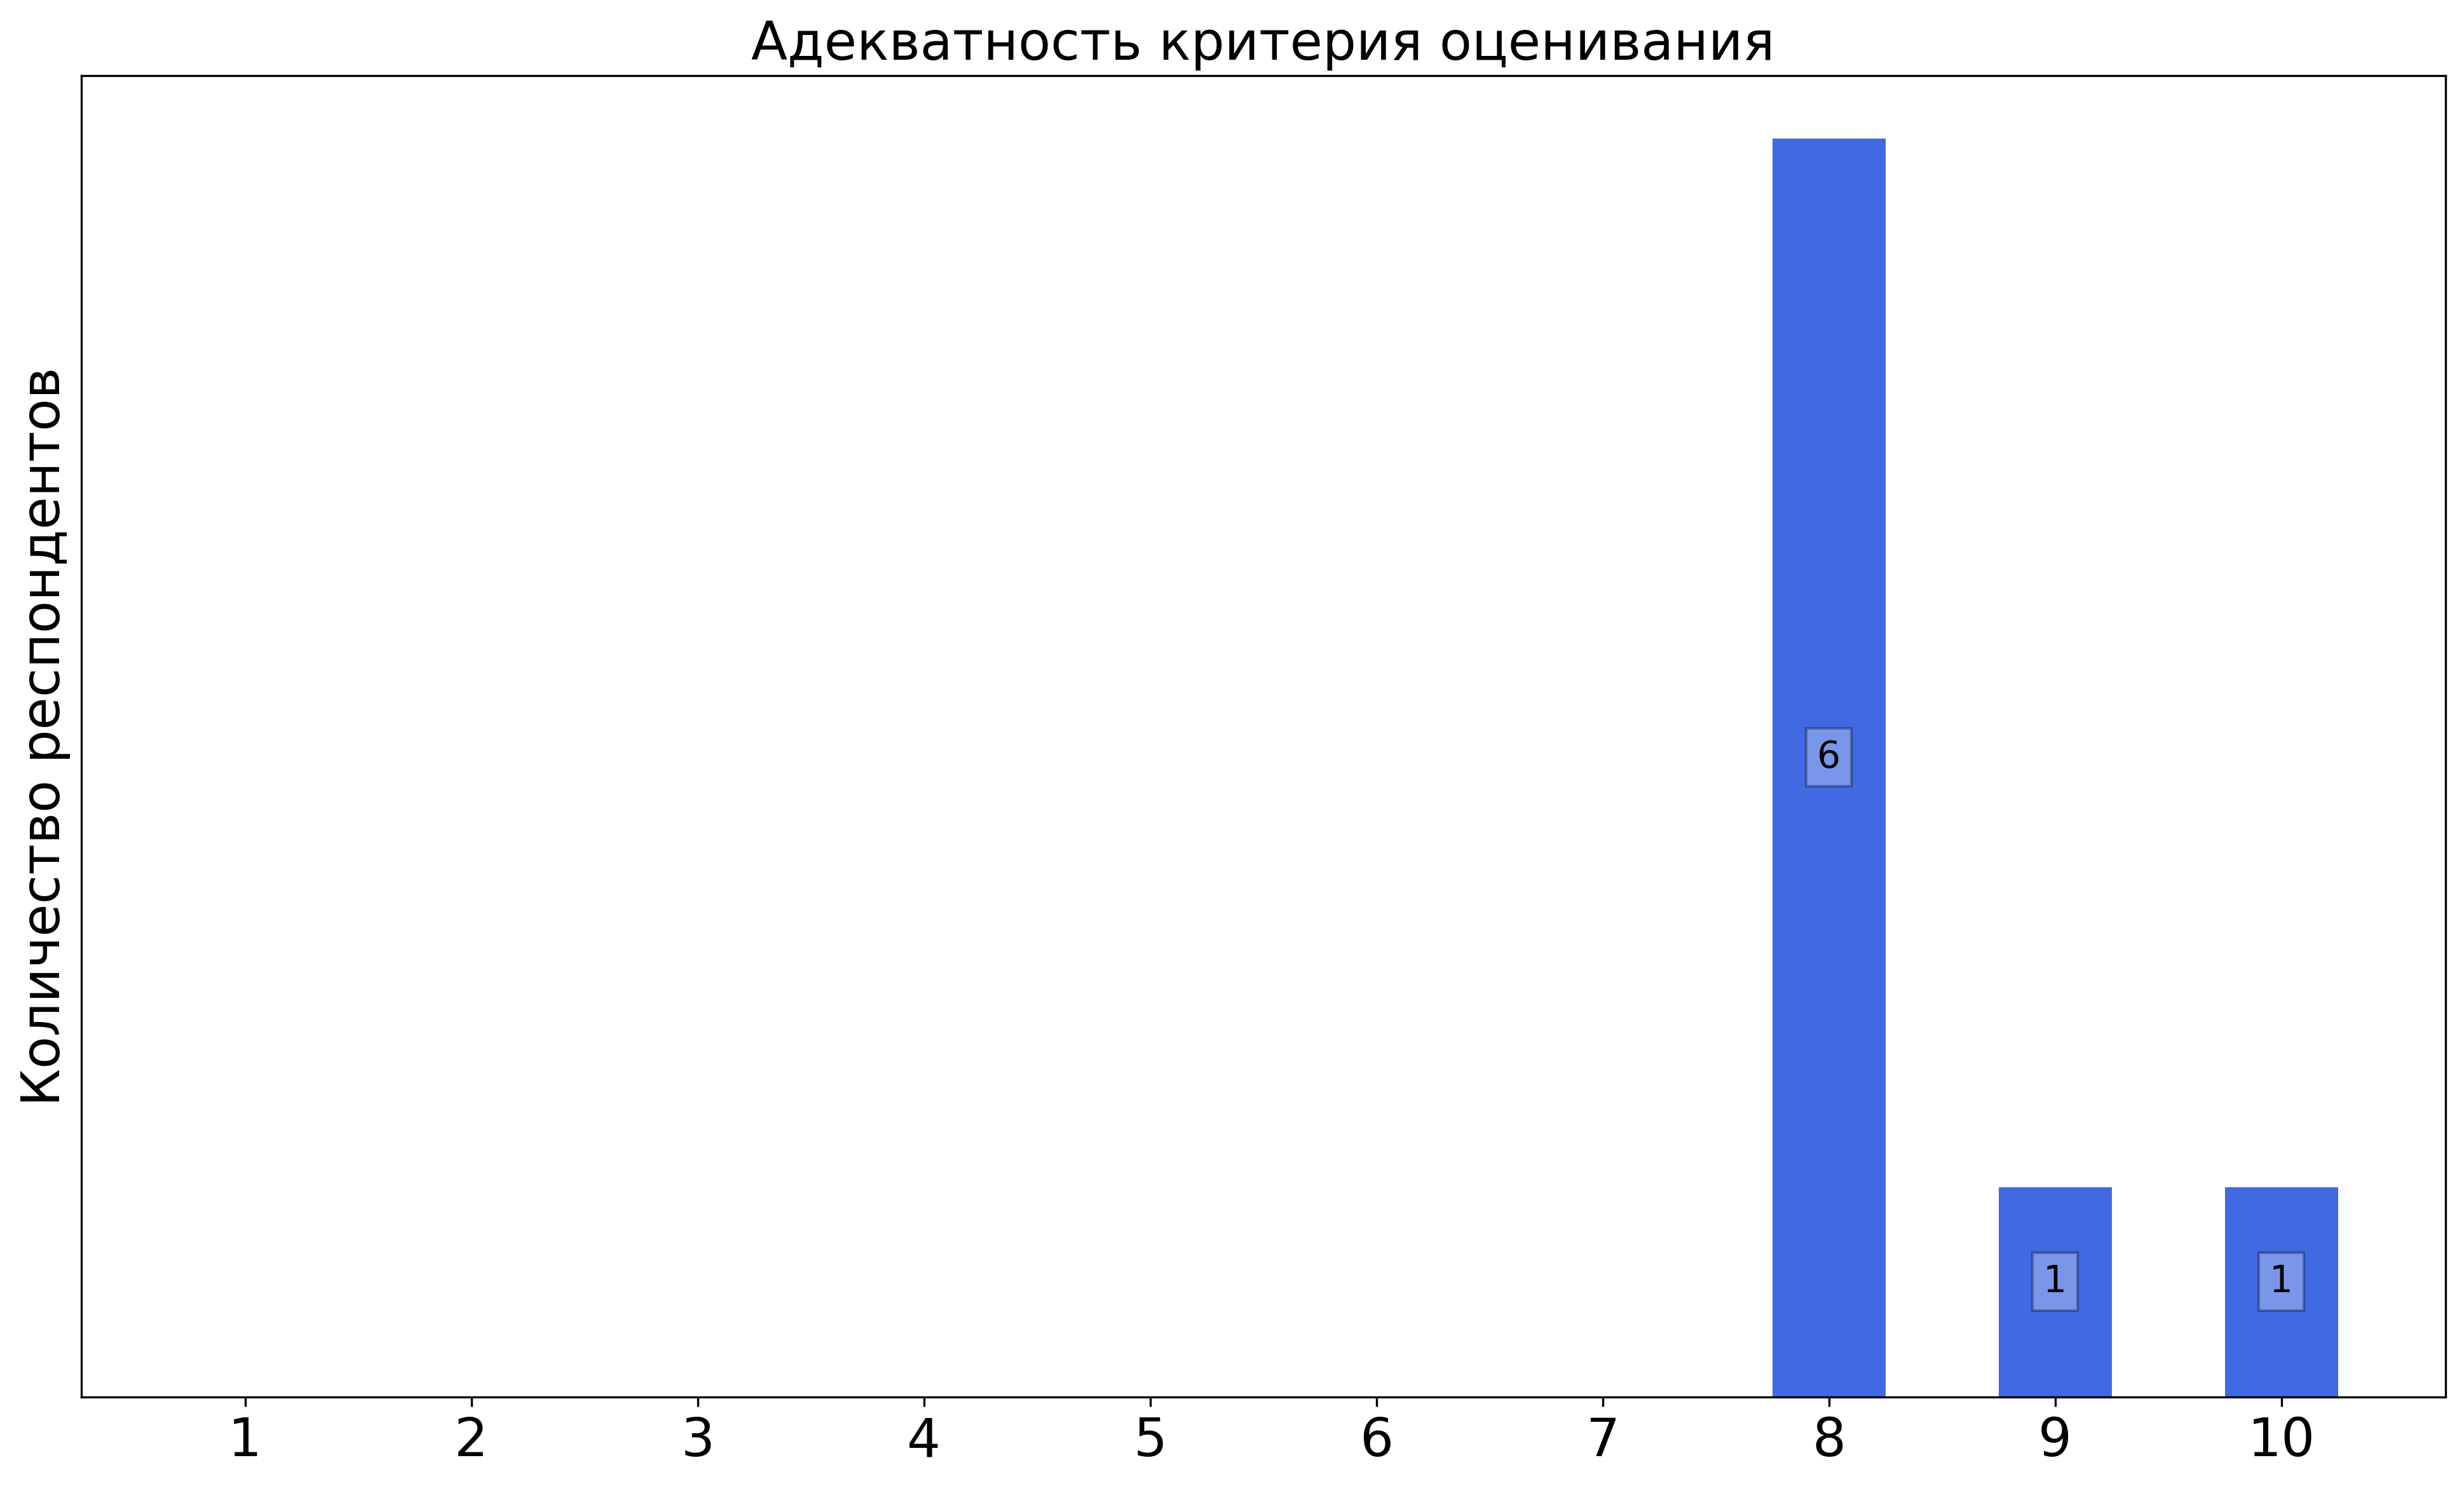
\includegraphics[width=\textwidth]{images/1 course/Общая физика - механика/labniks-marks-Долгих Е.А.-1.png}
            \end{subfigure}
            \begin{subfigure}[b]{0.45\textwidth}
                \centering
                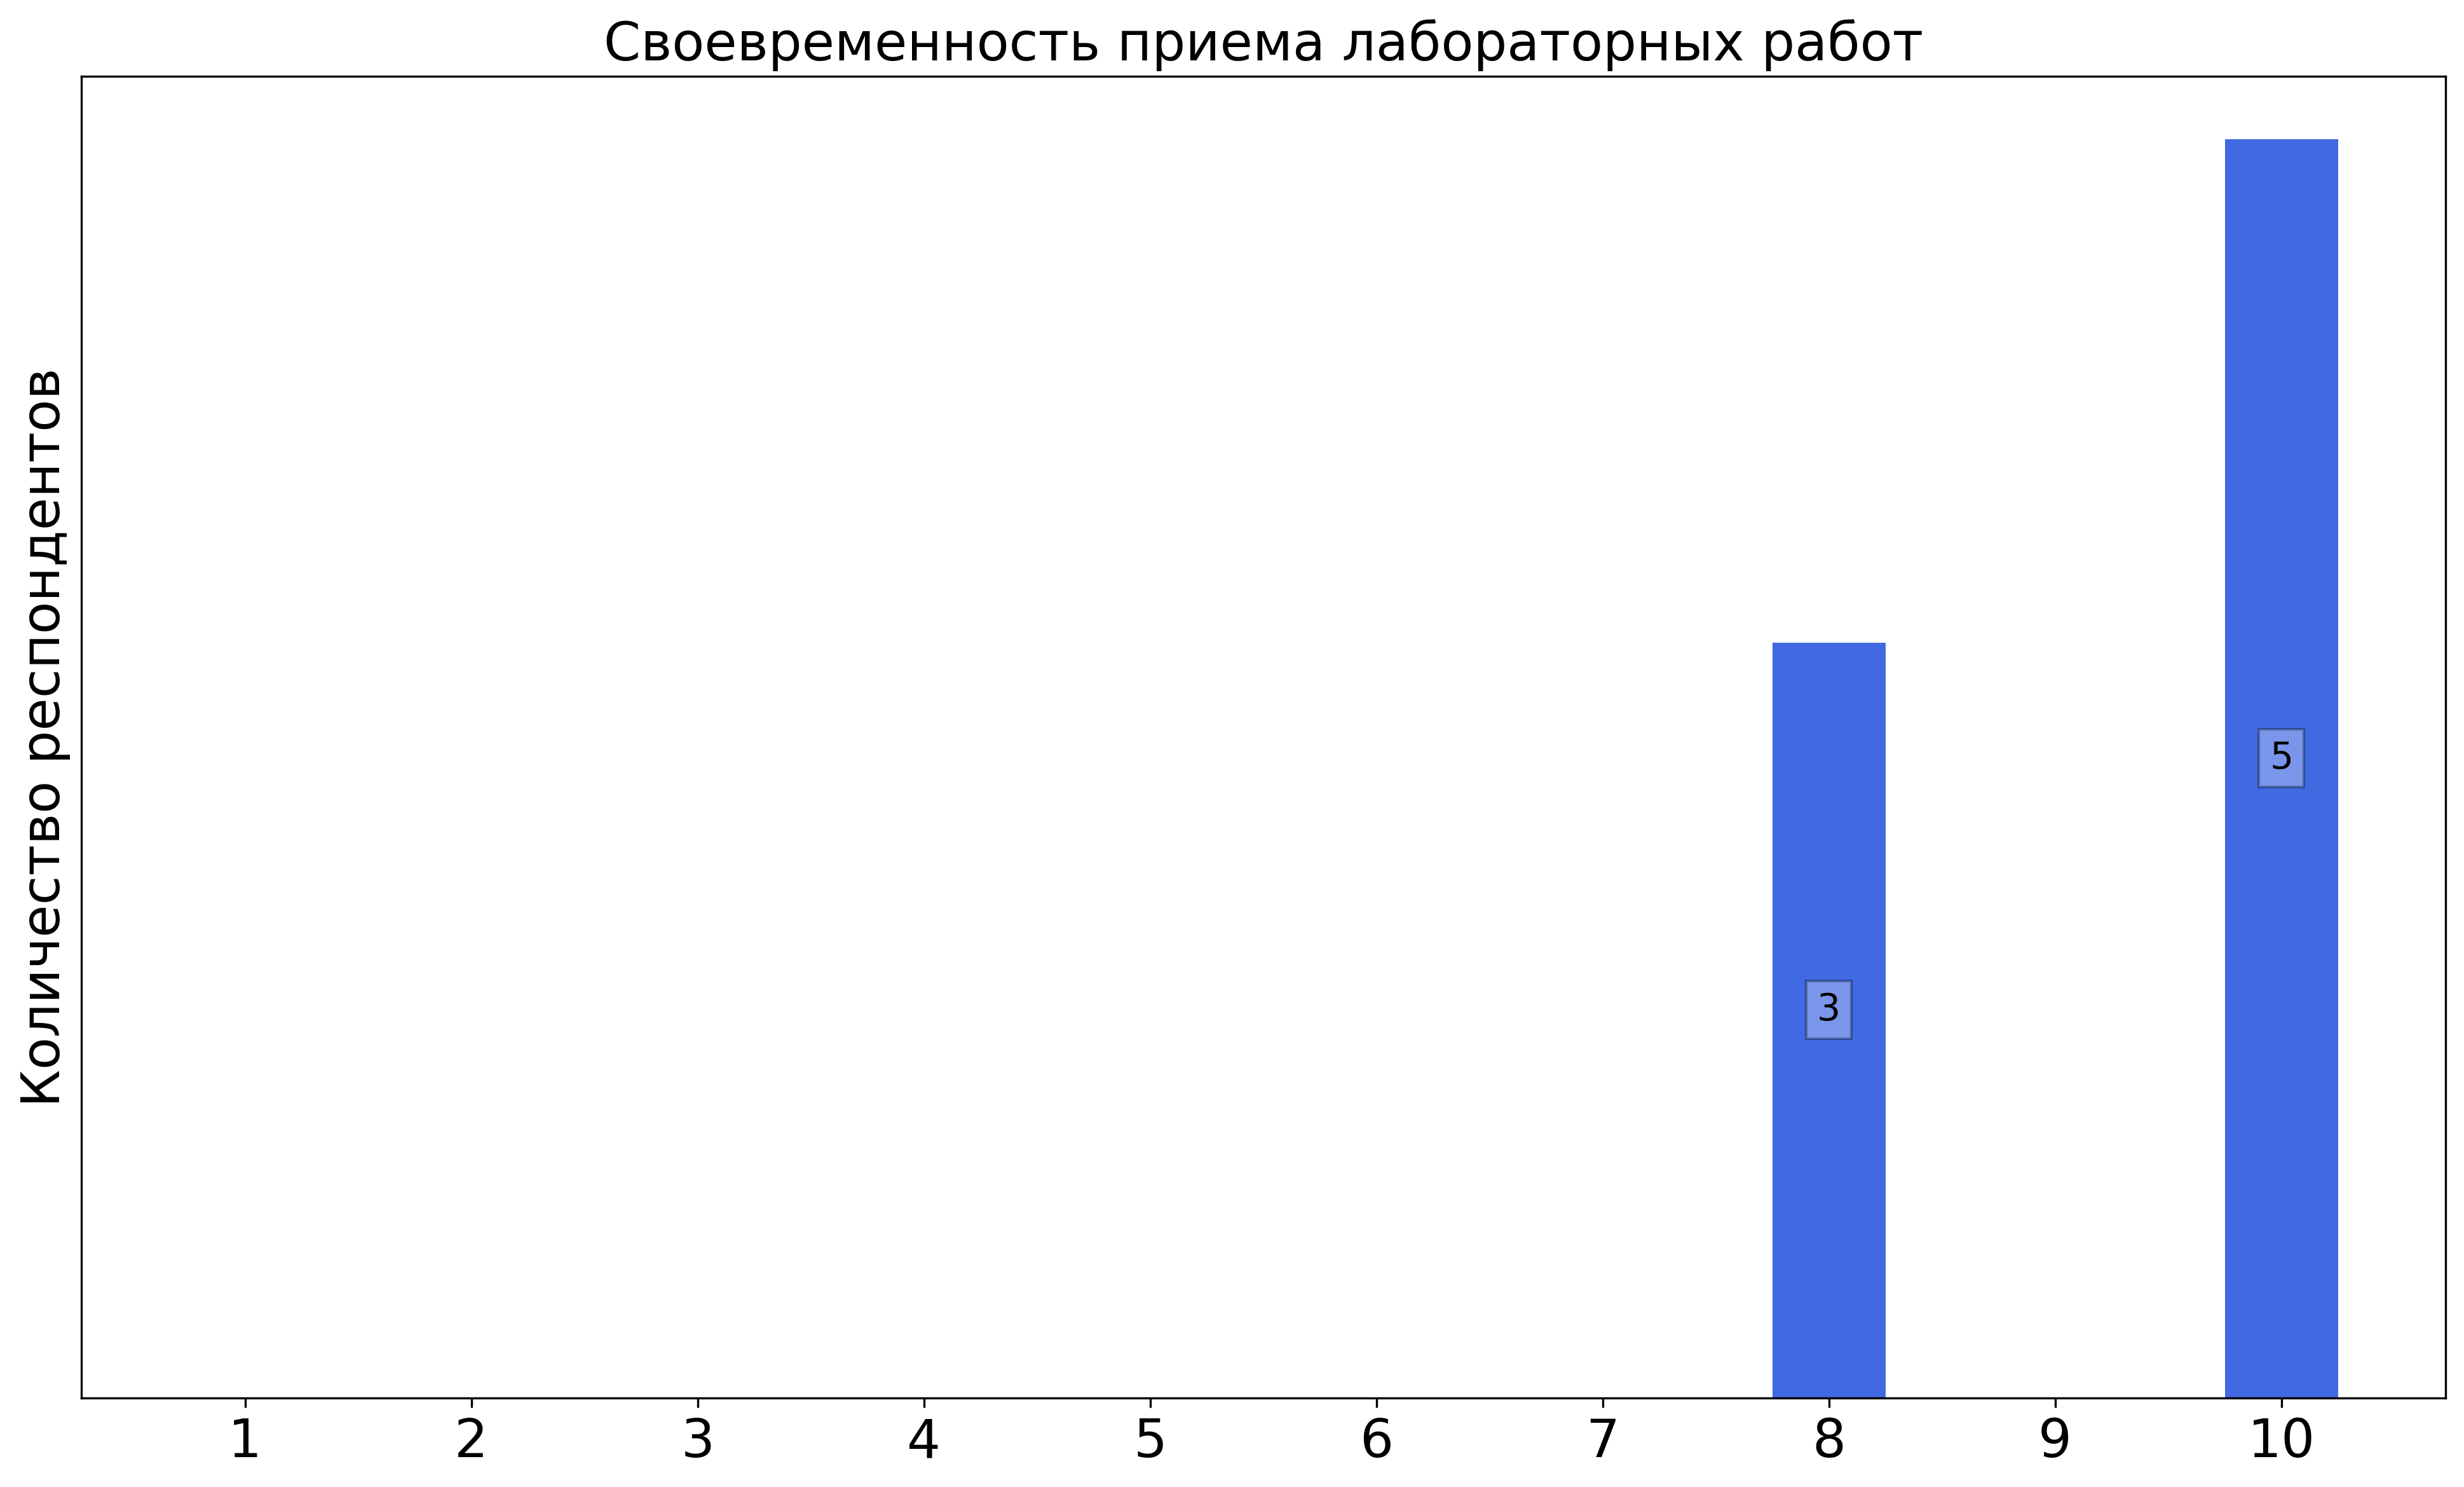
\includegraphics[width=\textwidth]{images/1 course/Общая физика - механика/labniks-marks-Долгих Е.А.-2.png}
            \end{subfigure}
            \begin{subfigure}[b]{0.45\textwidth}
                \centering
                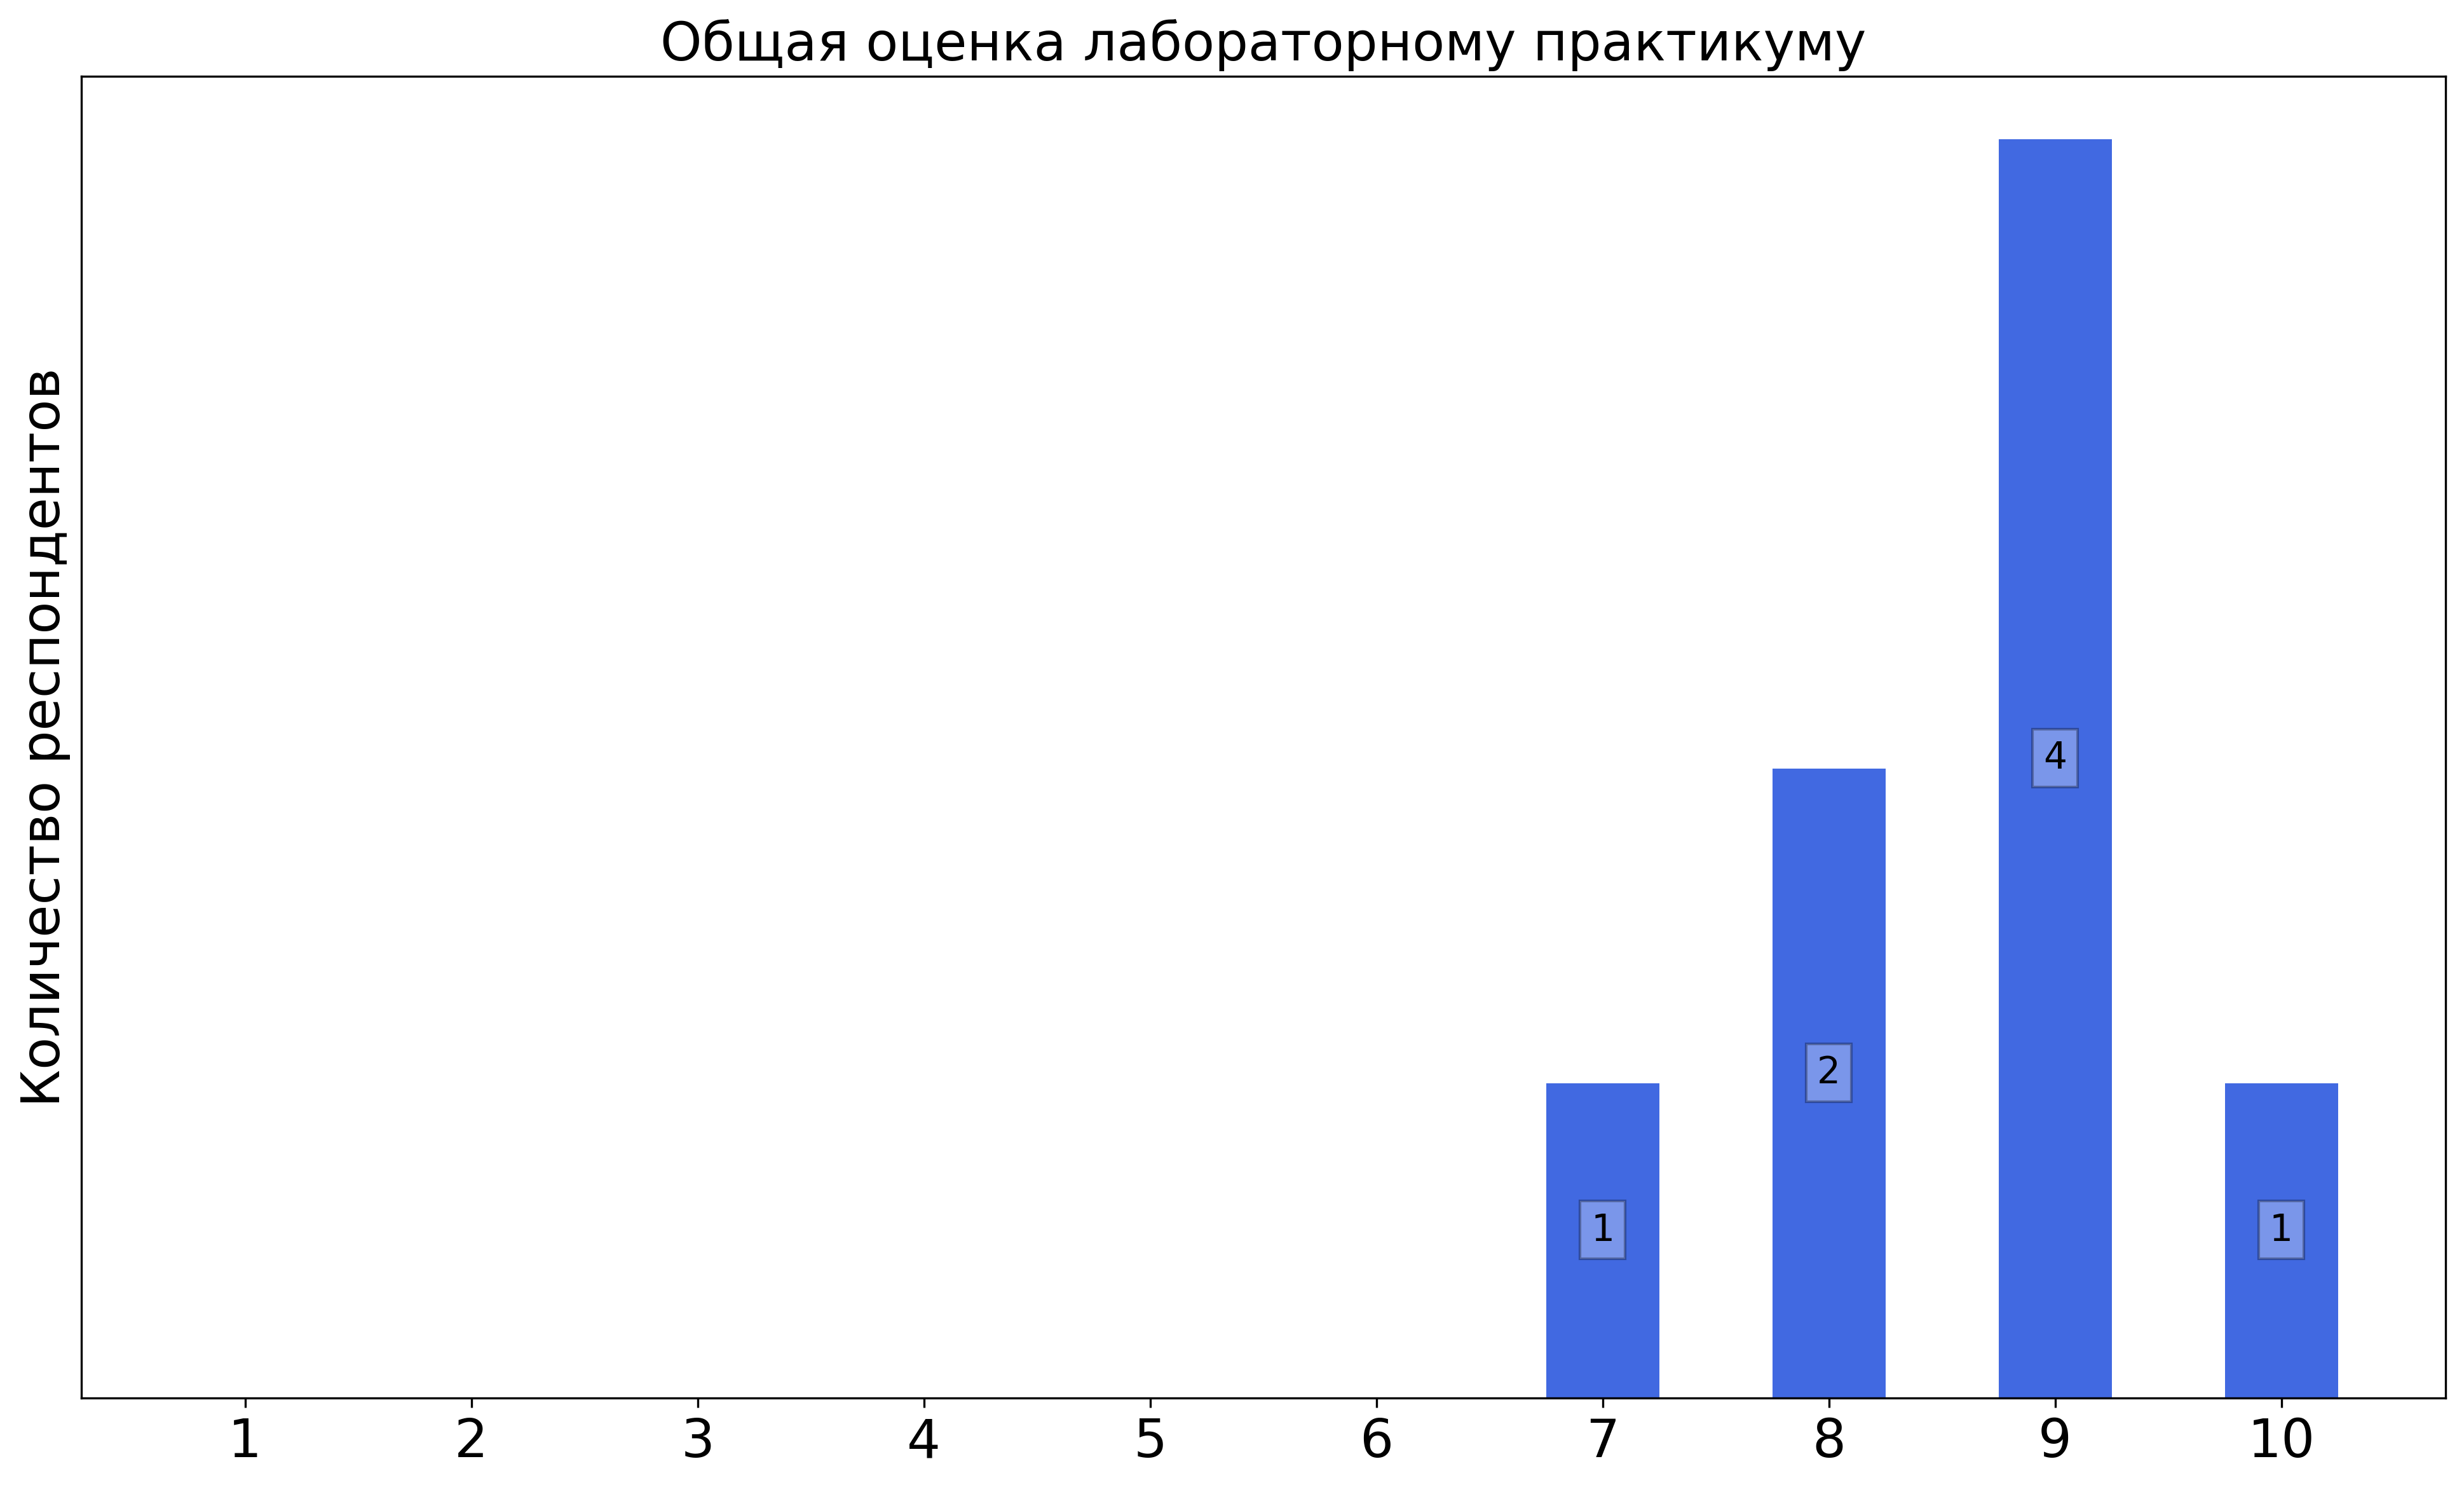
\includegraphics[width=\textwidth]{images/1 course/Общая физика - механика/labniks-marks-Долгих Е.А.-3.png}
            \end{subfigure}	
            \caption{Оценки респондентов о качестве преподавания лабораторных работ}
        \end{figure}

        \textbf{Комментарии студентов о преподавателе\protect\footnote{сохранены оригинальные орфография и пунктуация}}
            \begin{commentbox} 
                Хороший преподаватель, на вопросы отвечает в целом. Есть возможность донести работы позже. Помогла с вопросом по выбору. 
            \end{commentbox} 


    \subsubsection{Отзыв студентов о лабораторных работах. Преподаватель: Корнева А.А.}
        \begin{figure}[H]
            \centering
            \begin{subfigure}[b]{0.45\textwidth}
                \centering
                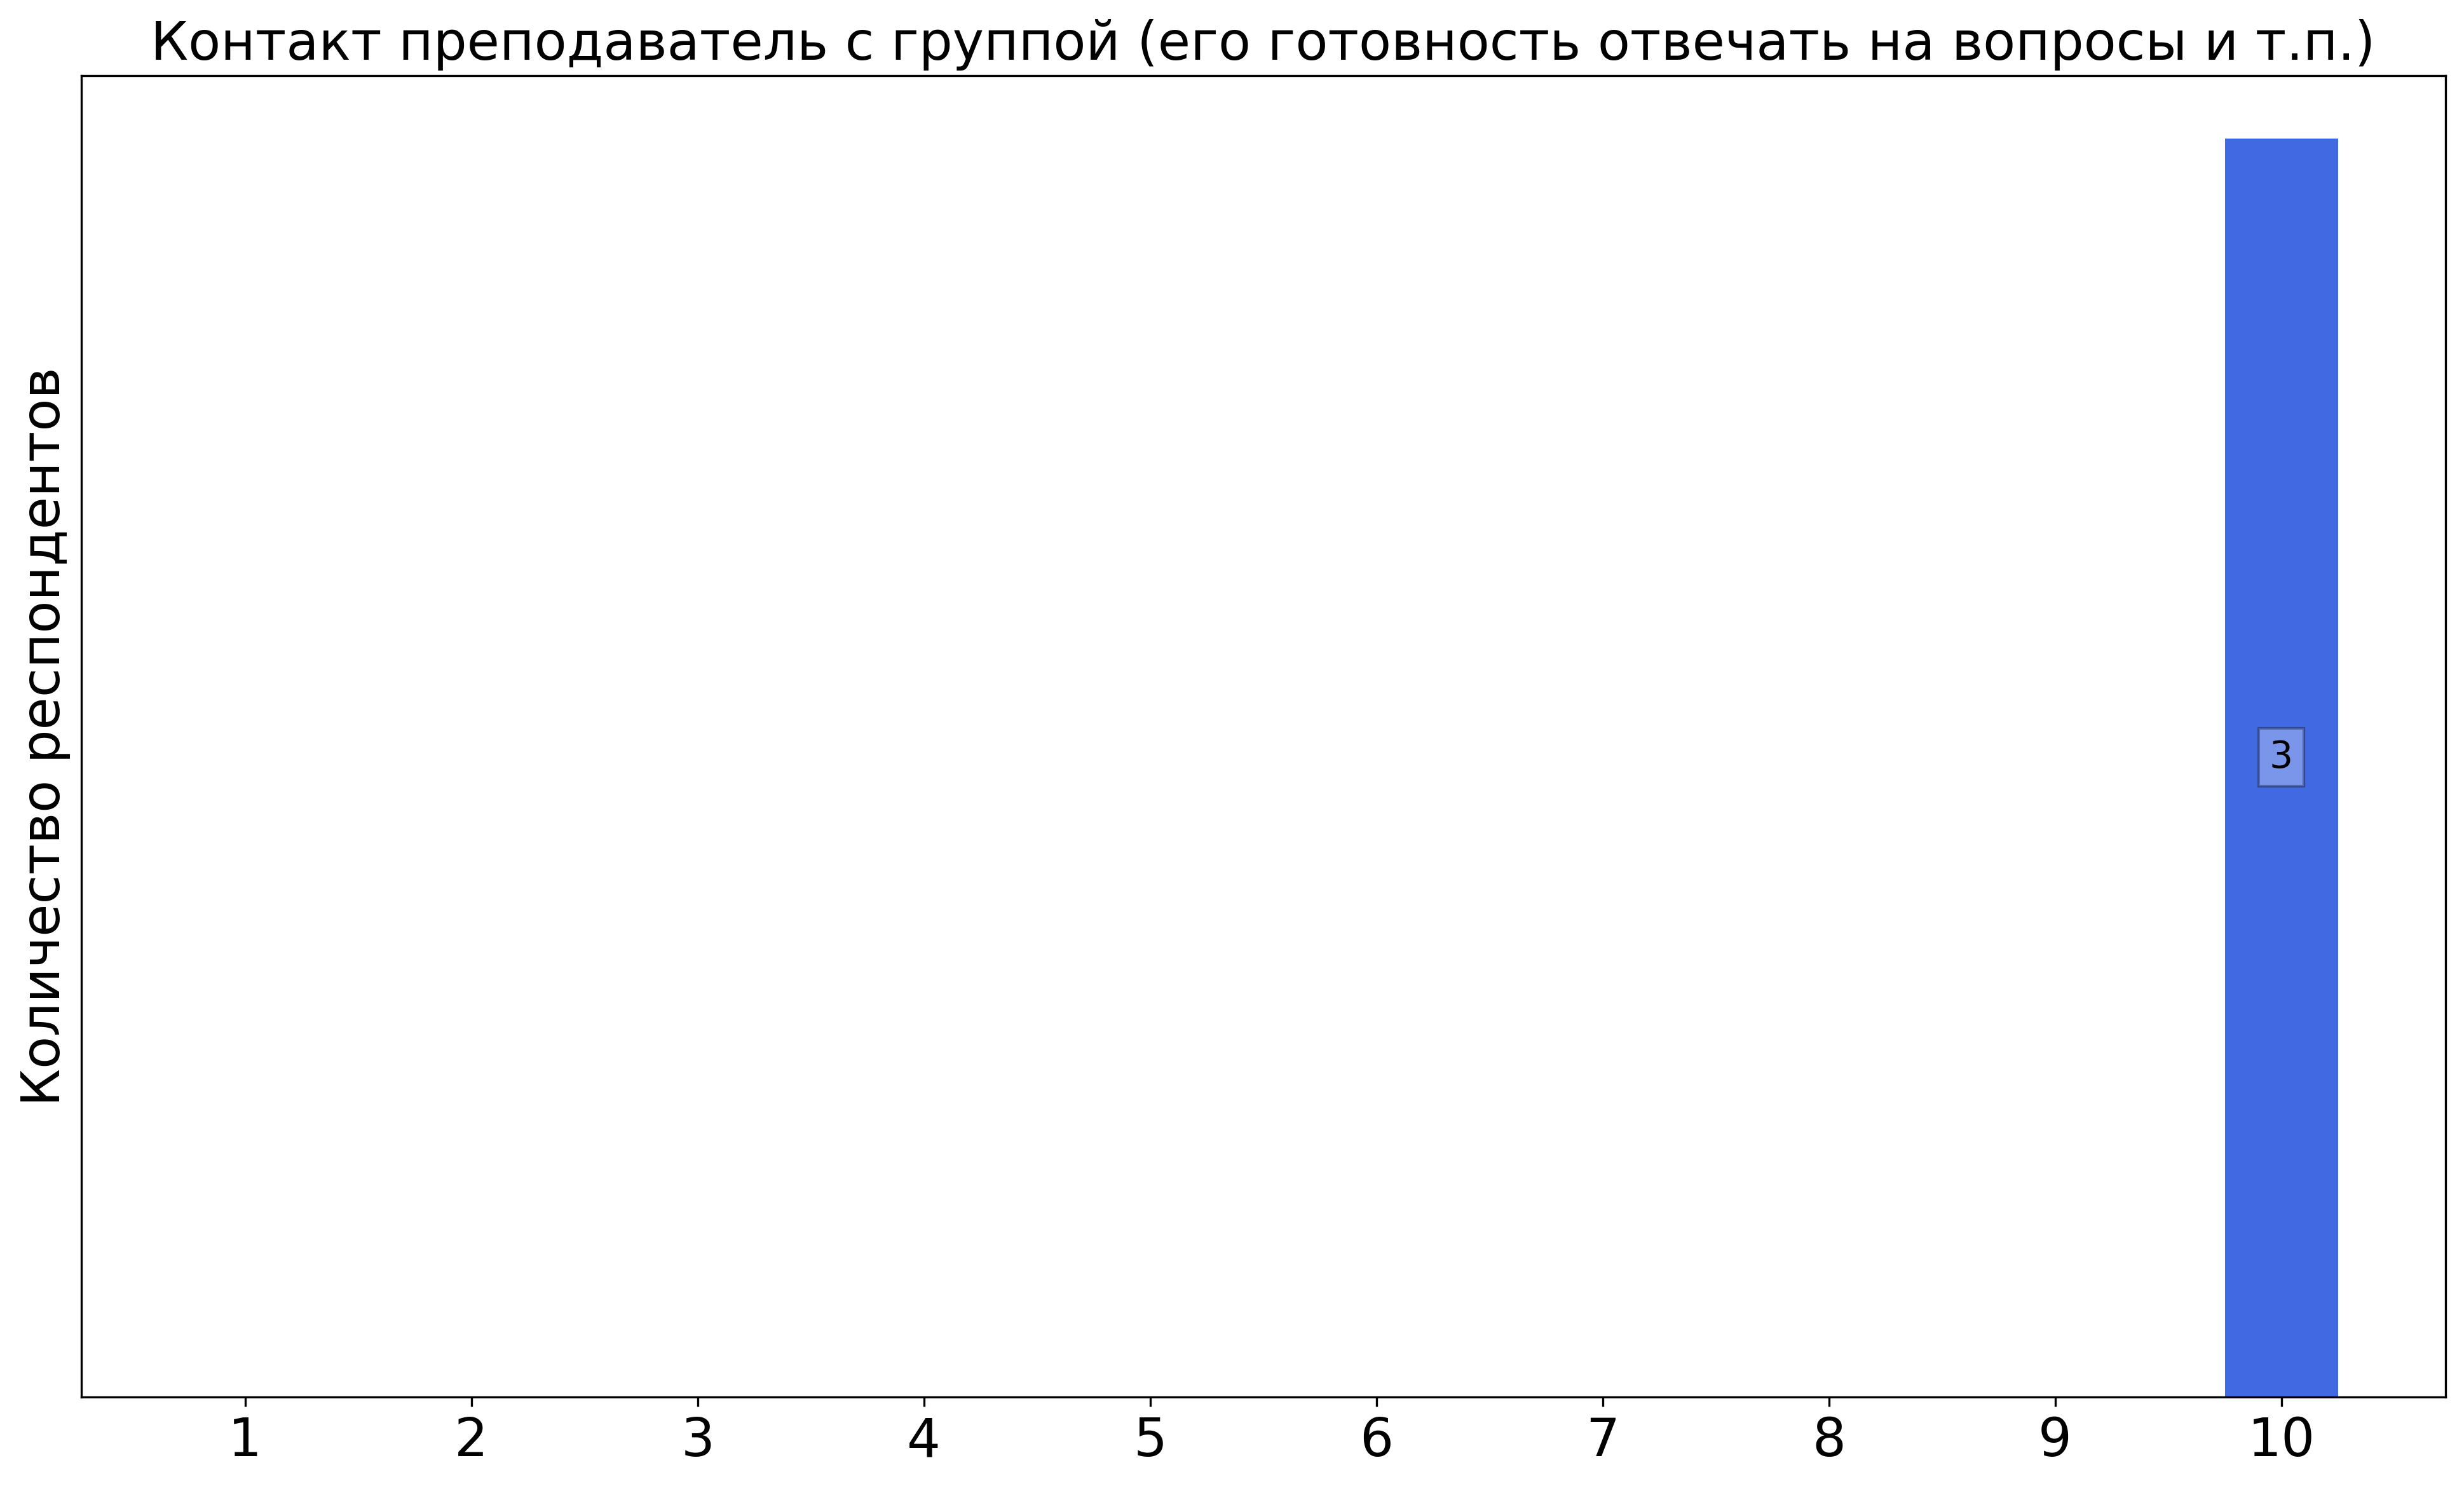
\includegraphics[width=\textwidth]{images/1 course/Общая физика - механика/labniks-marks-Корнева А.А.-0.png}
            \end{subfigure}
            \begin{subfigure}[b]{0.45\textwidth}
                \centering
                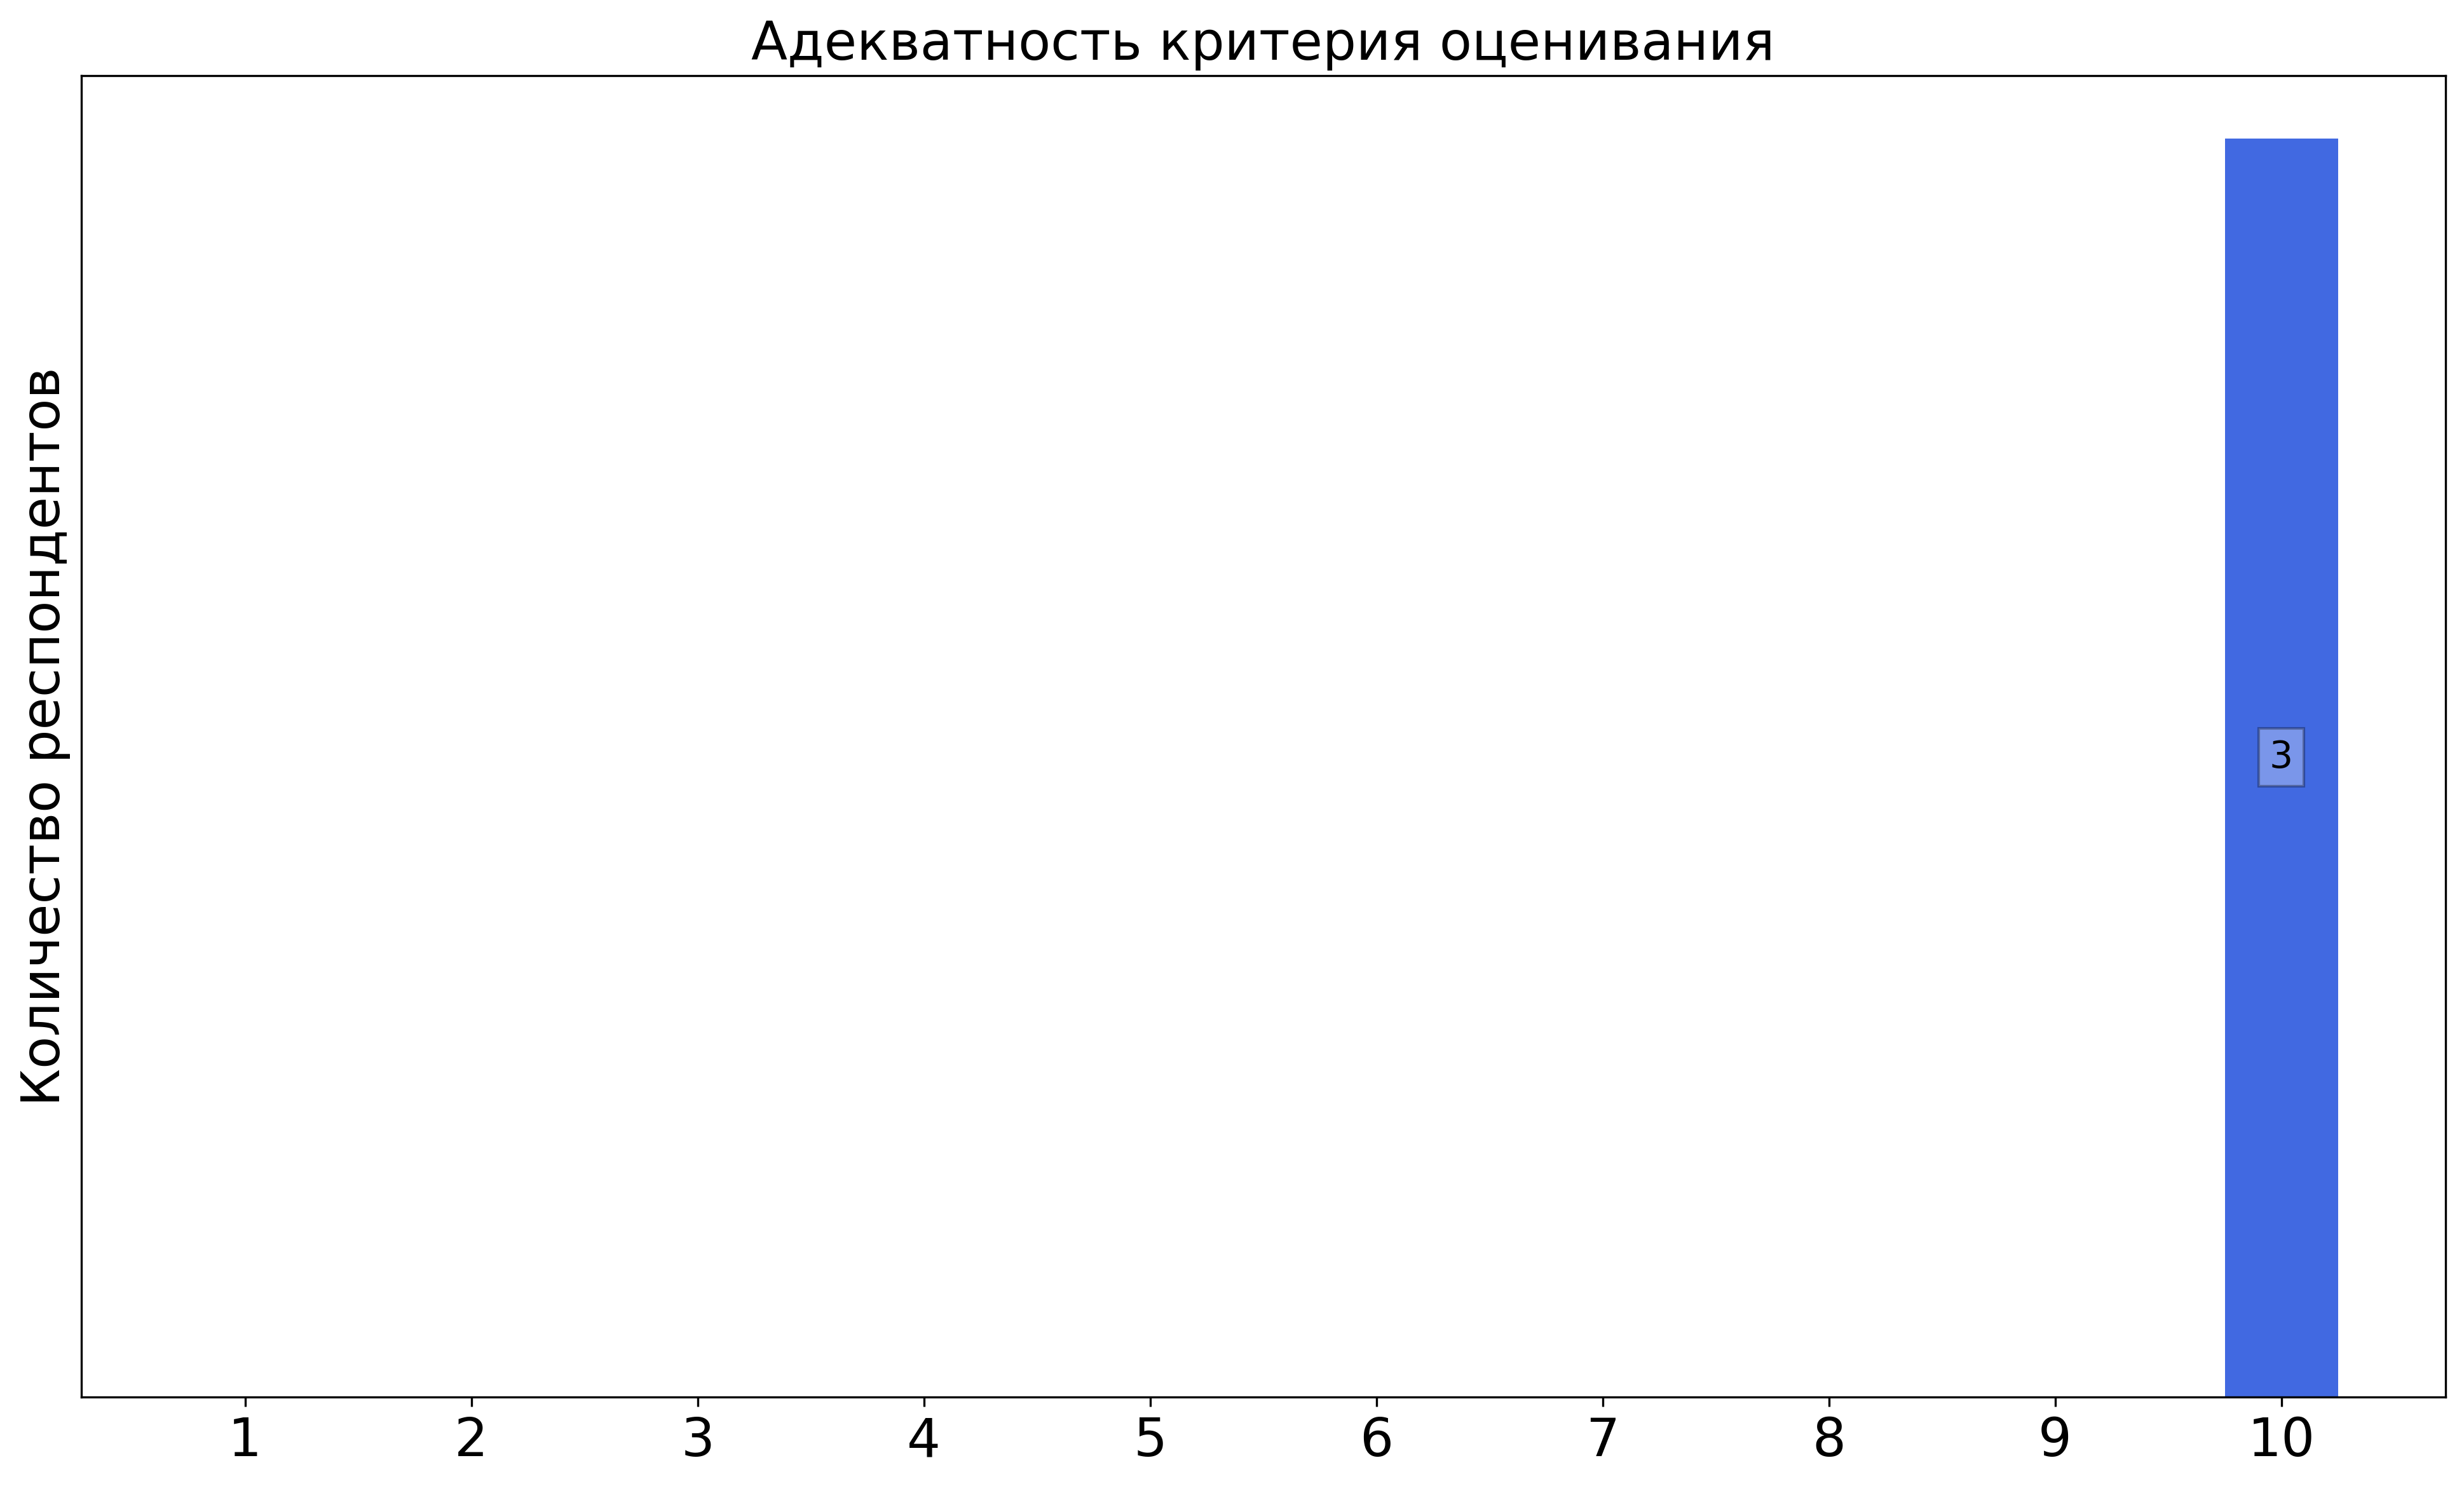
\includegraphics[width=\textwidth]{images/1 course/Общая физика - механика/labniks-marks-Корнева А.А.-1.png}
            \end{subfigure}
            \begin{subfigure}[b]{0.45\textwidth}
                \centering
                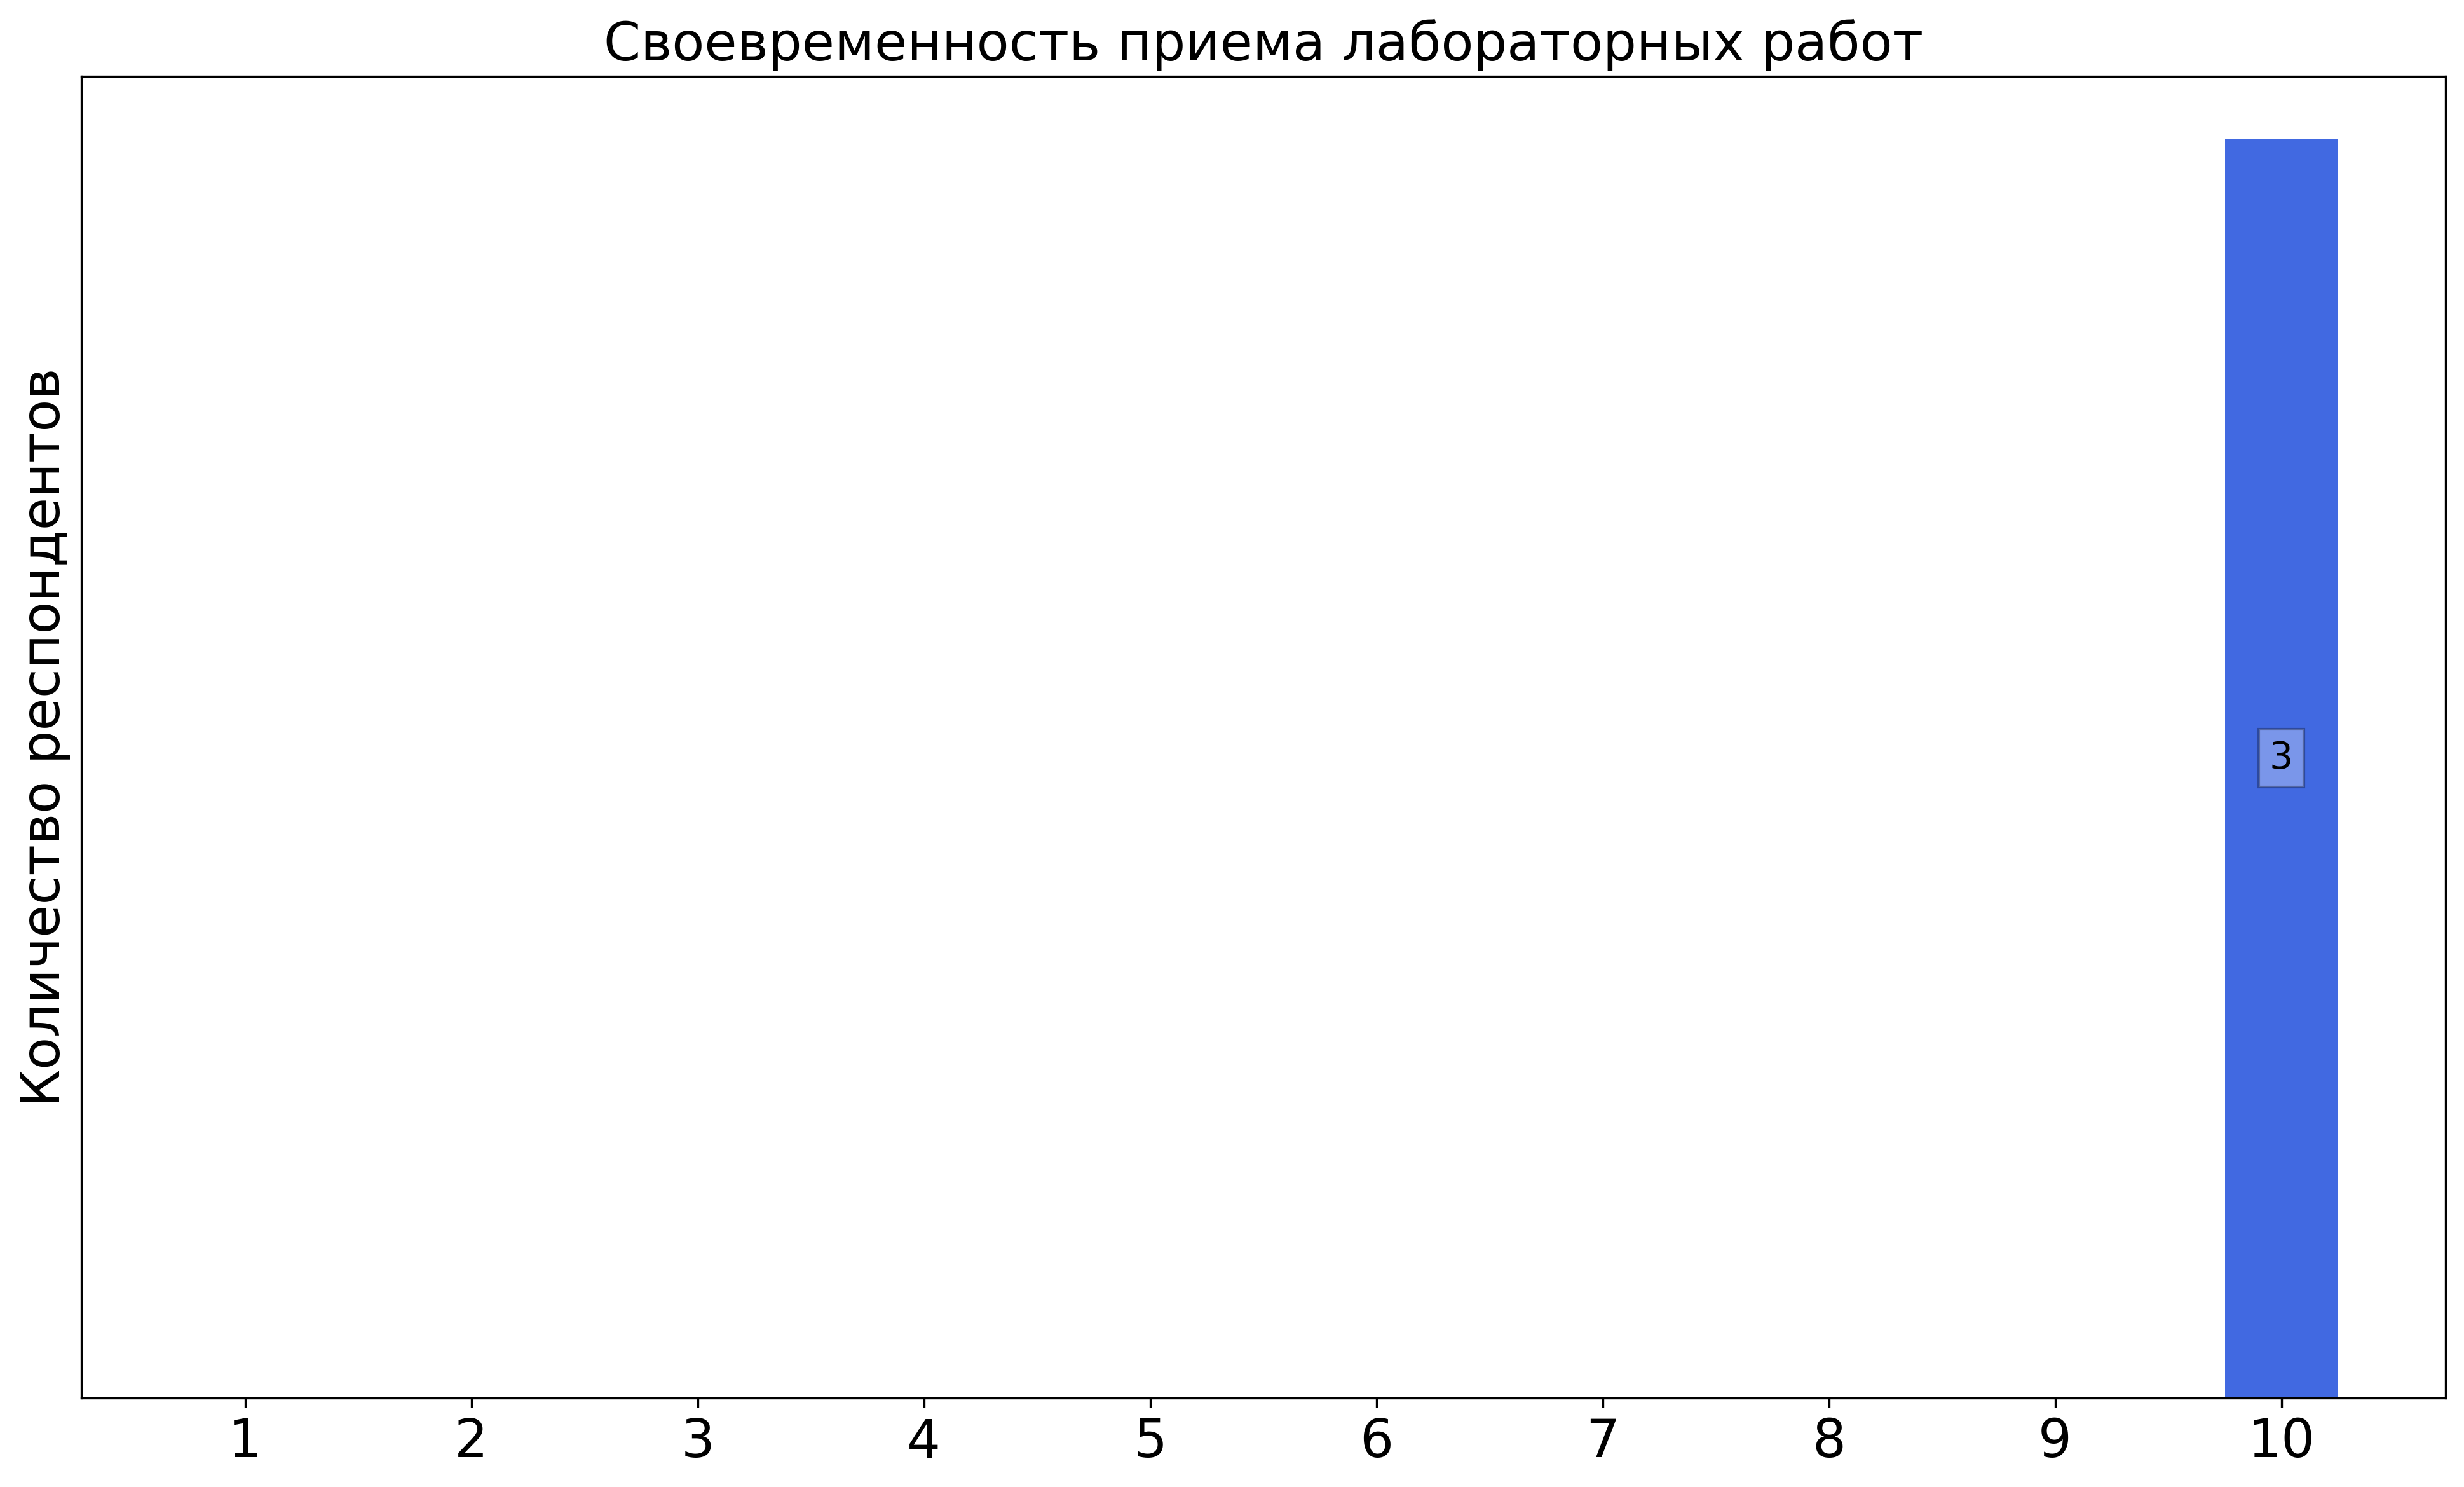
\includegraphics[width=\textwidth]{images/1 course/Общая физика - механика/labniks-marks-Корнева А.А.-2.png}
            \end{subfigure}
            \begin{subfigure}[b]{0.45\textwidth}
                \centering
                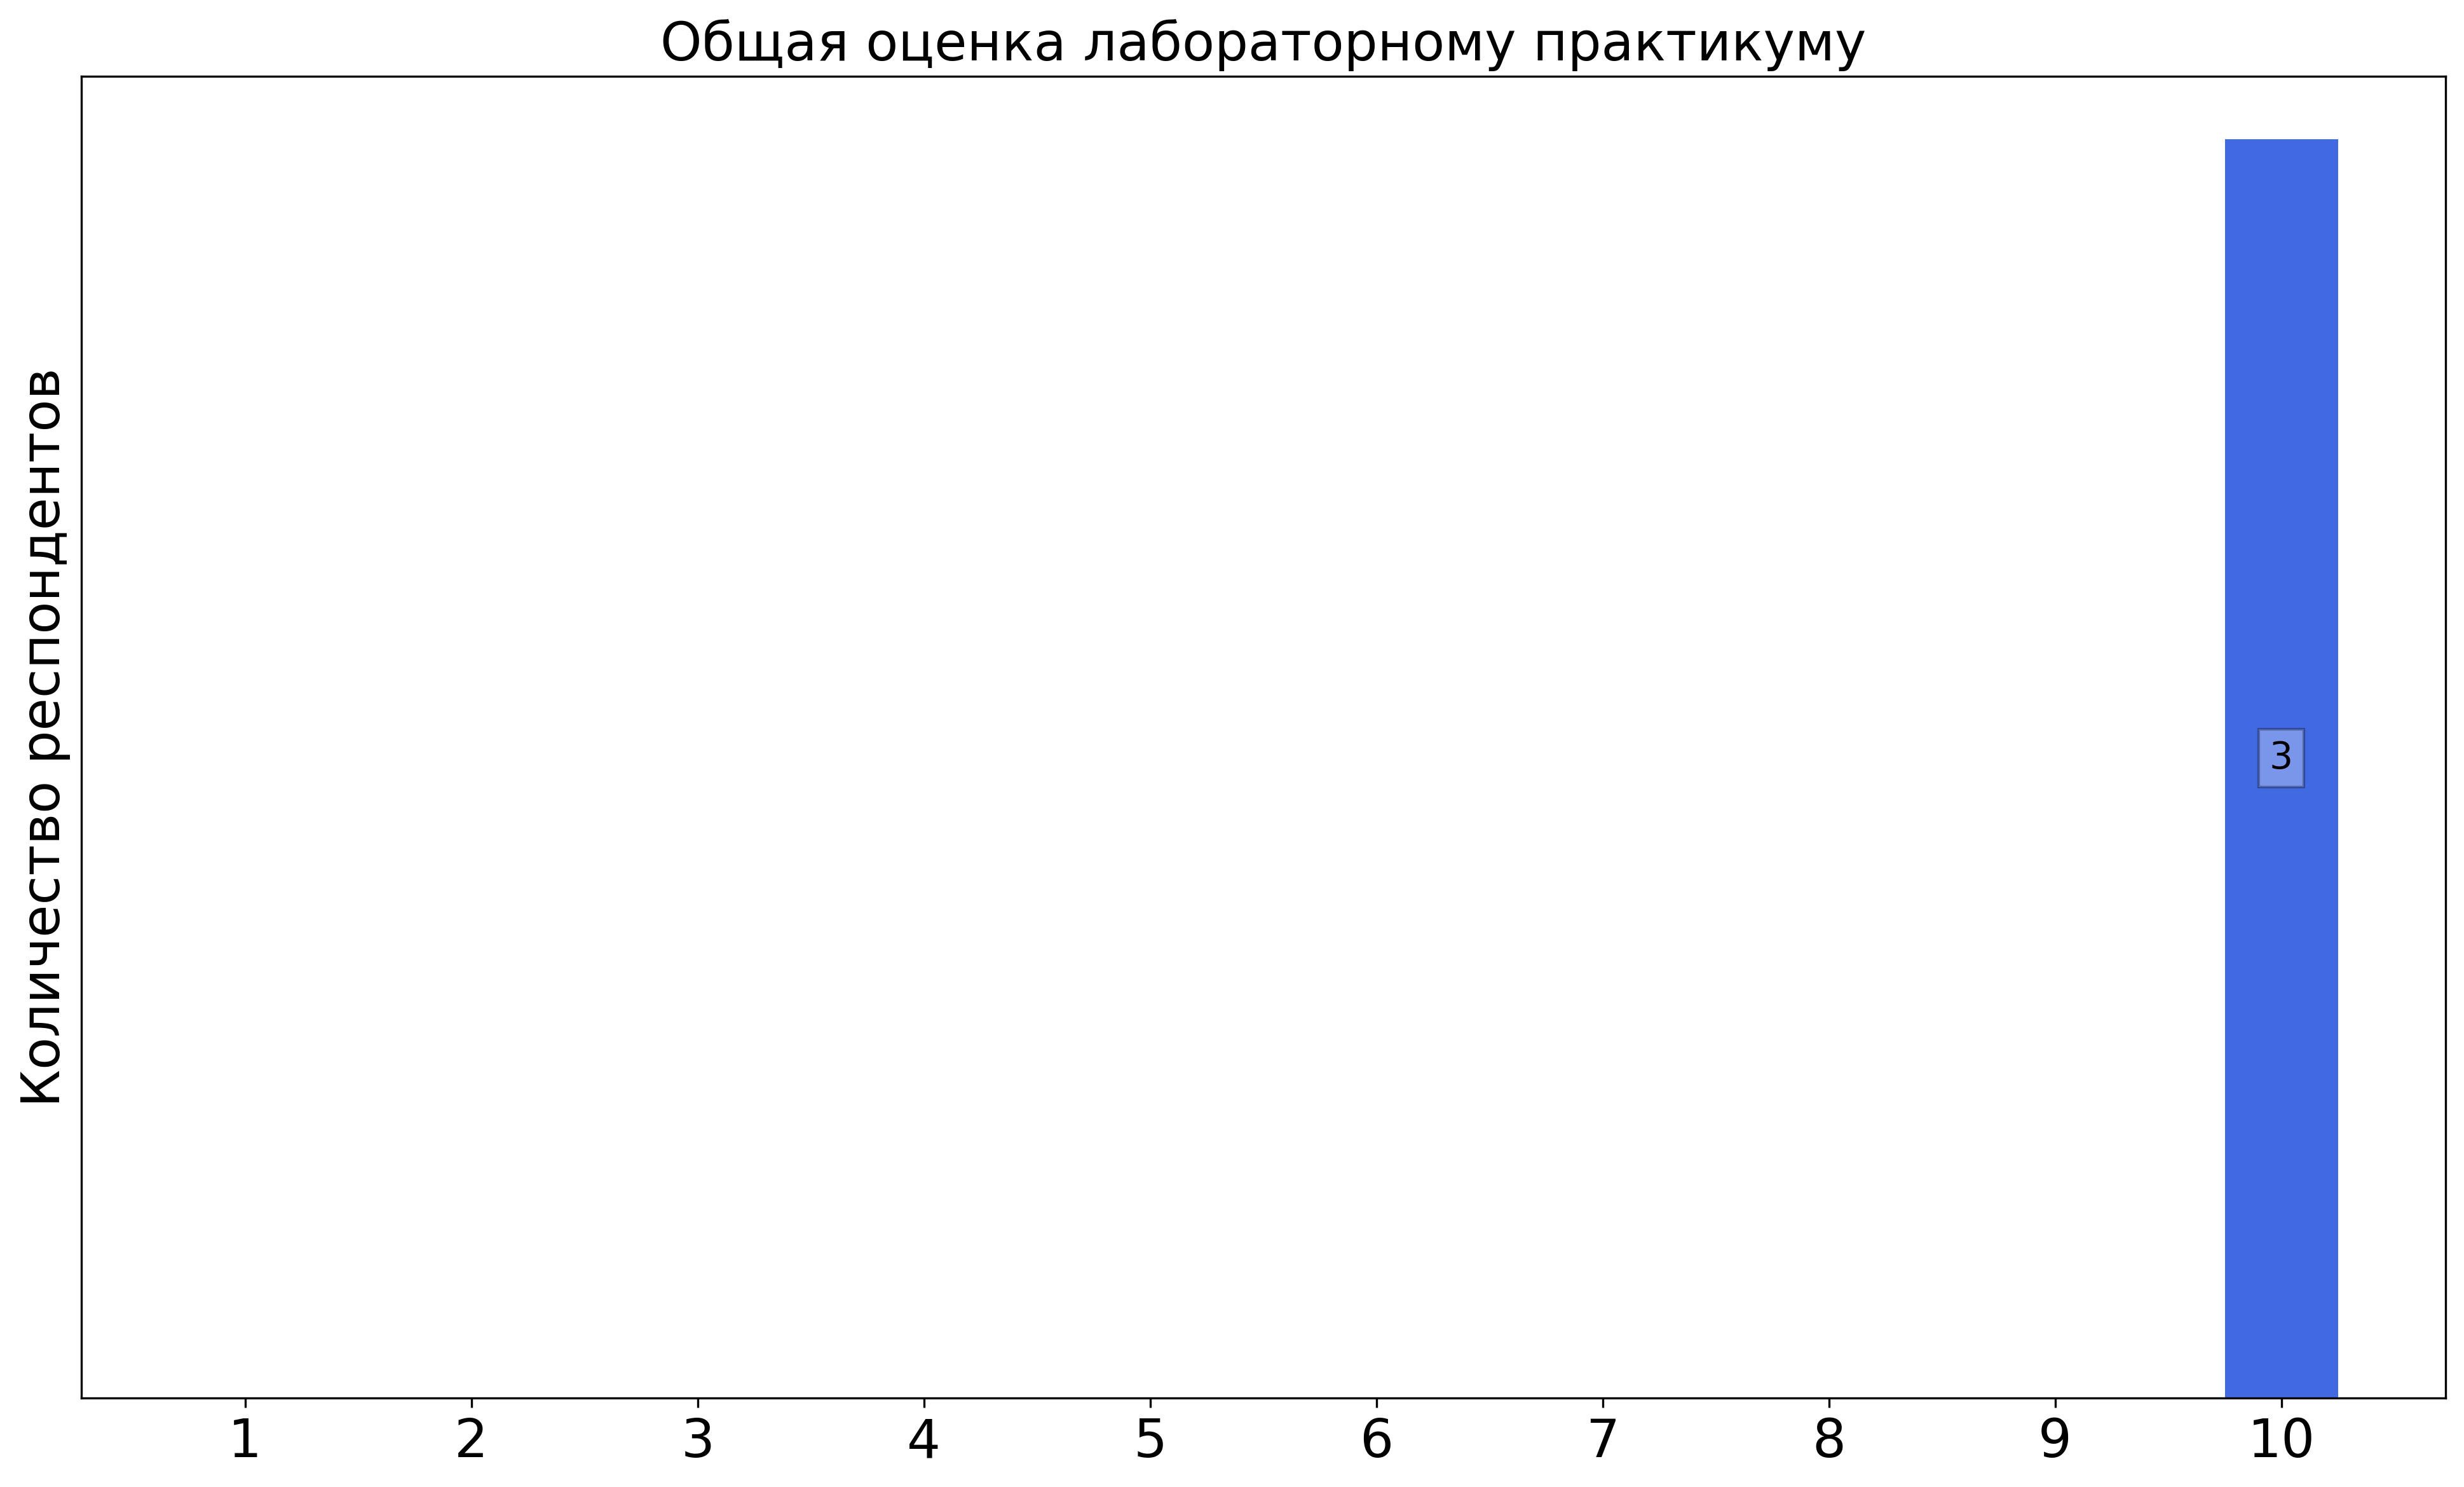
\includegraphics[width=\textwidth]{images/1 course/Общая физика - механика/labniks-marks-Корнева А.А.-3.png}
            \end{subfigure}	
            \caption{Оценки респондентов о качестве преподавания лабораторных работ}
        \end{figure}


    \subsubsection{Отзыв студентов о лабораторных работах. Преподаватель: Суханова Е.В.}
		\begin{figure}[H]
			\centering
			\begin{subfigure}[b]{0.45\textwidth}
				\centering
				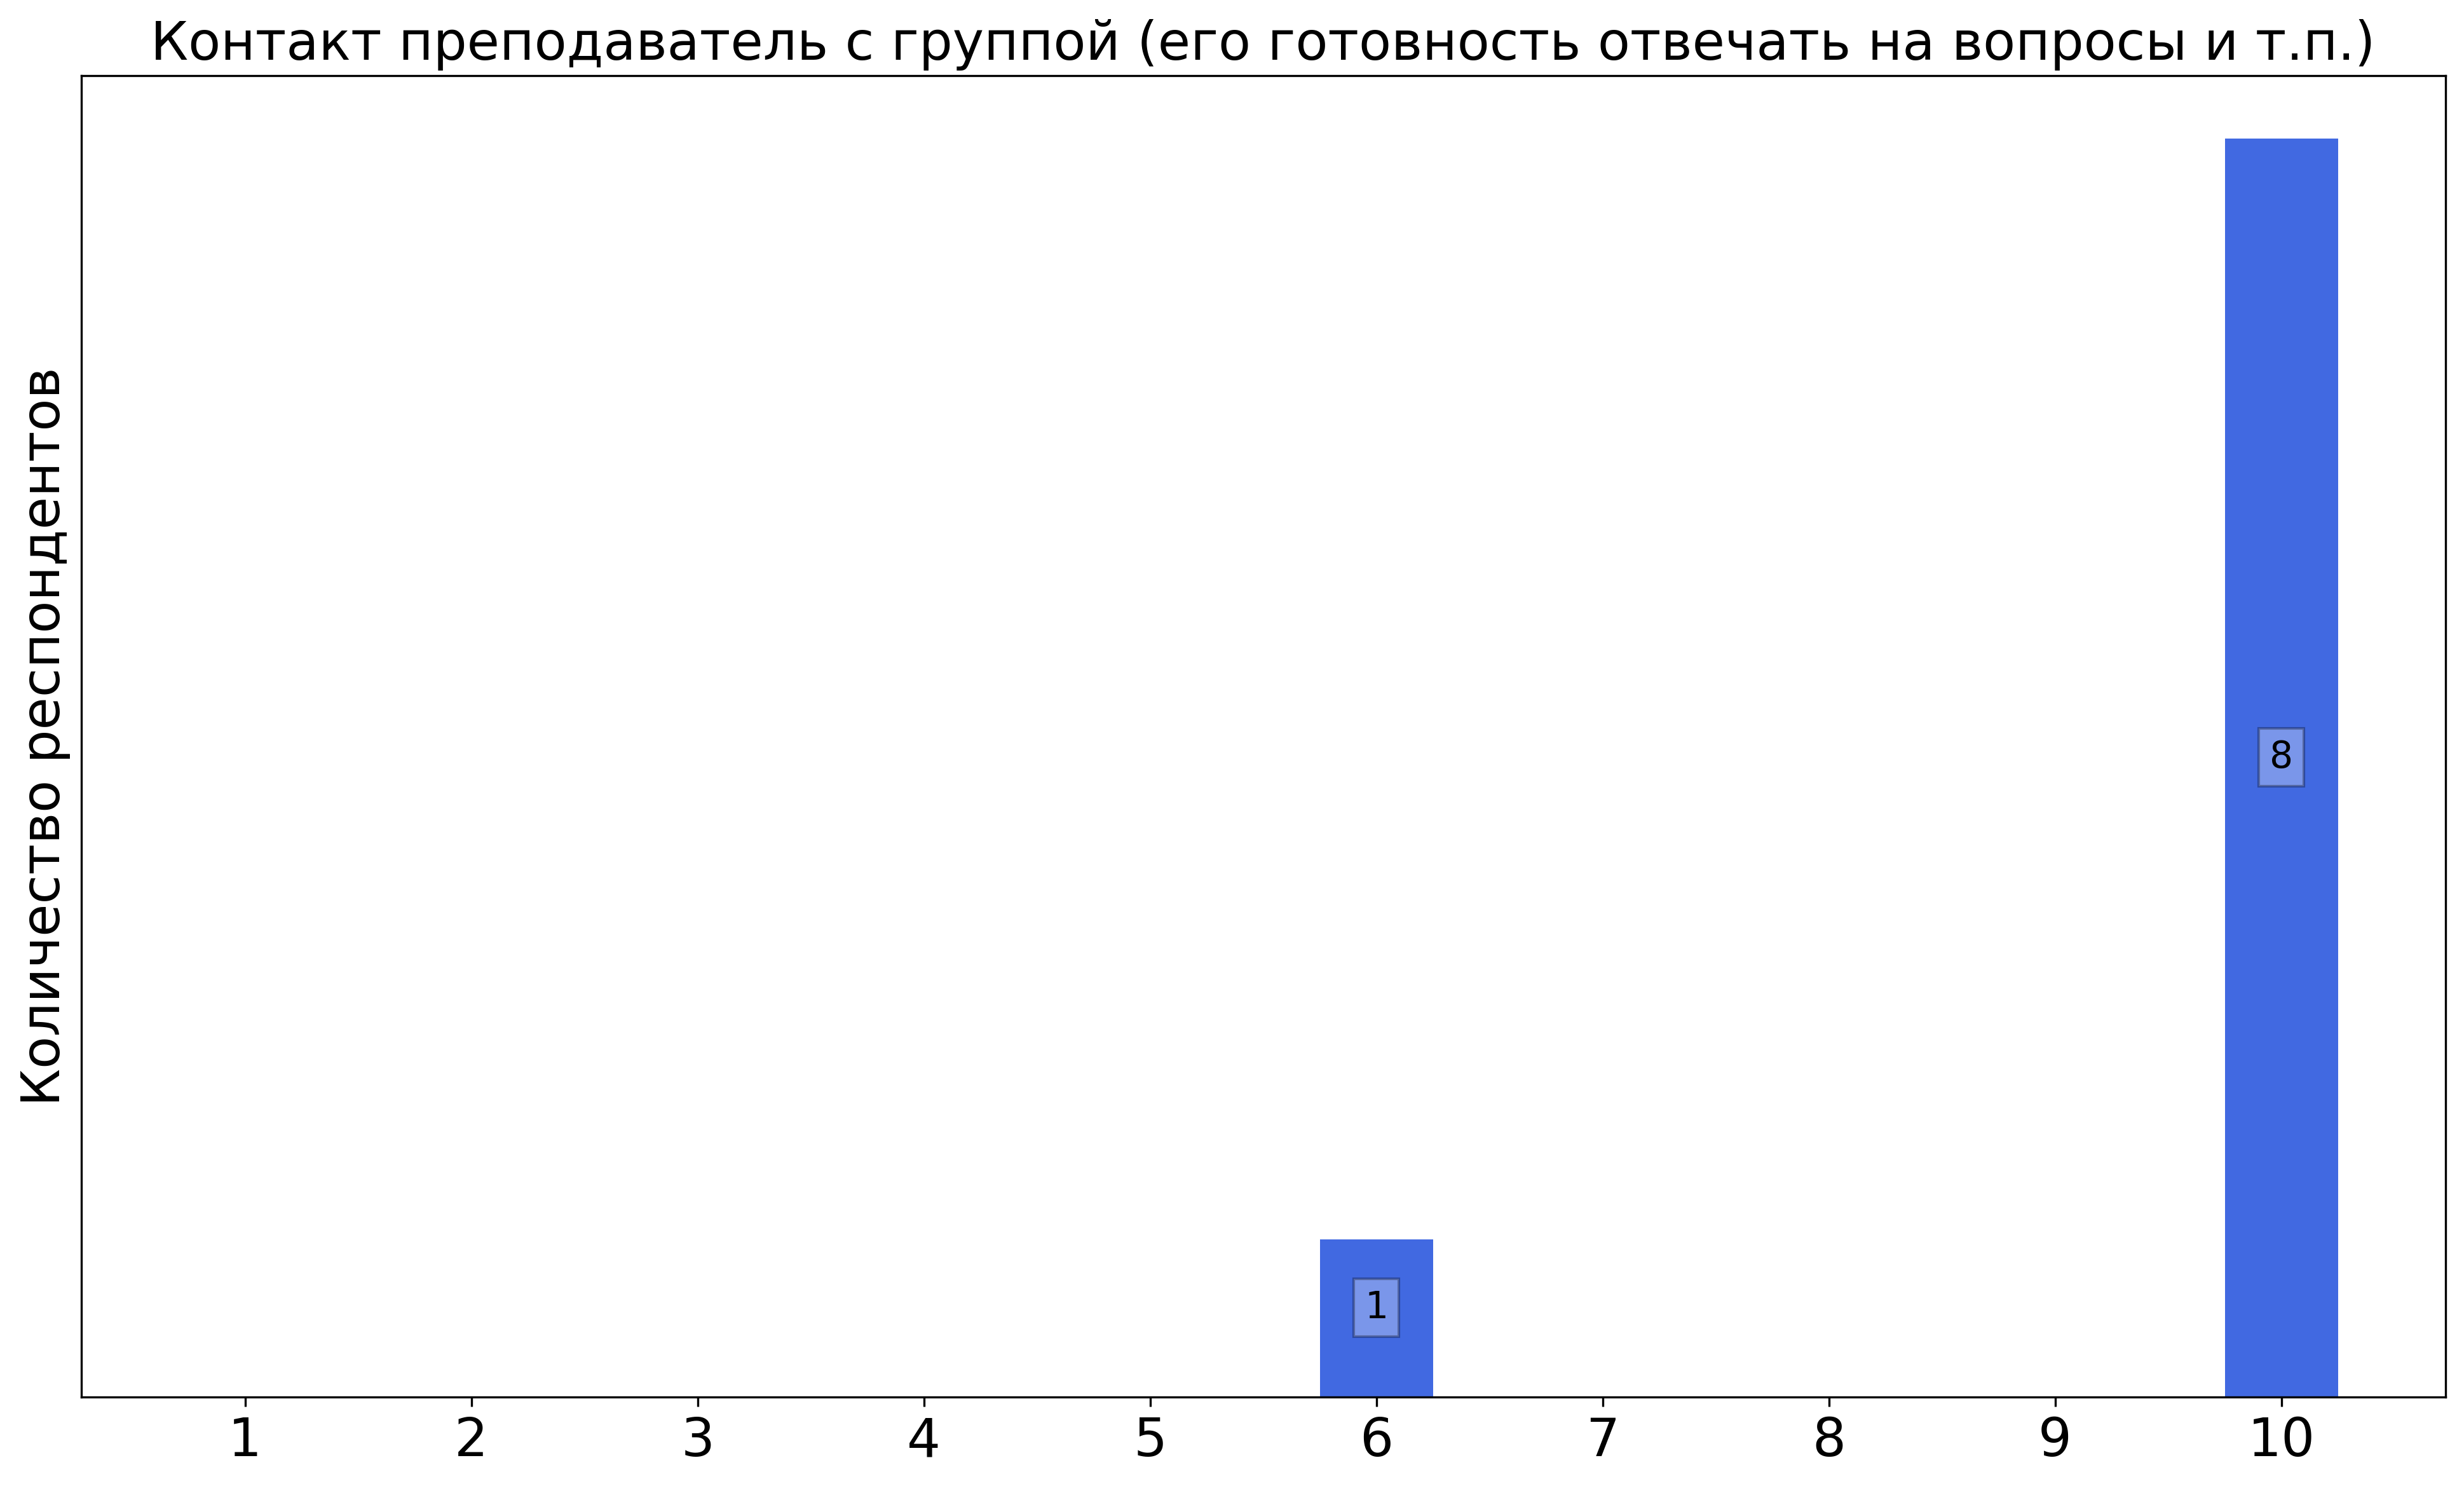
\includegraphics[width=\textwidth]{images/1 course/Общая физика - механика/labniks-marks-Суханова Е.В.-0.png}
			\end{subfigure}
			\begin{subfigure}[b]{0.45\textwidth}
				\centering
				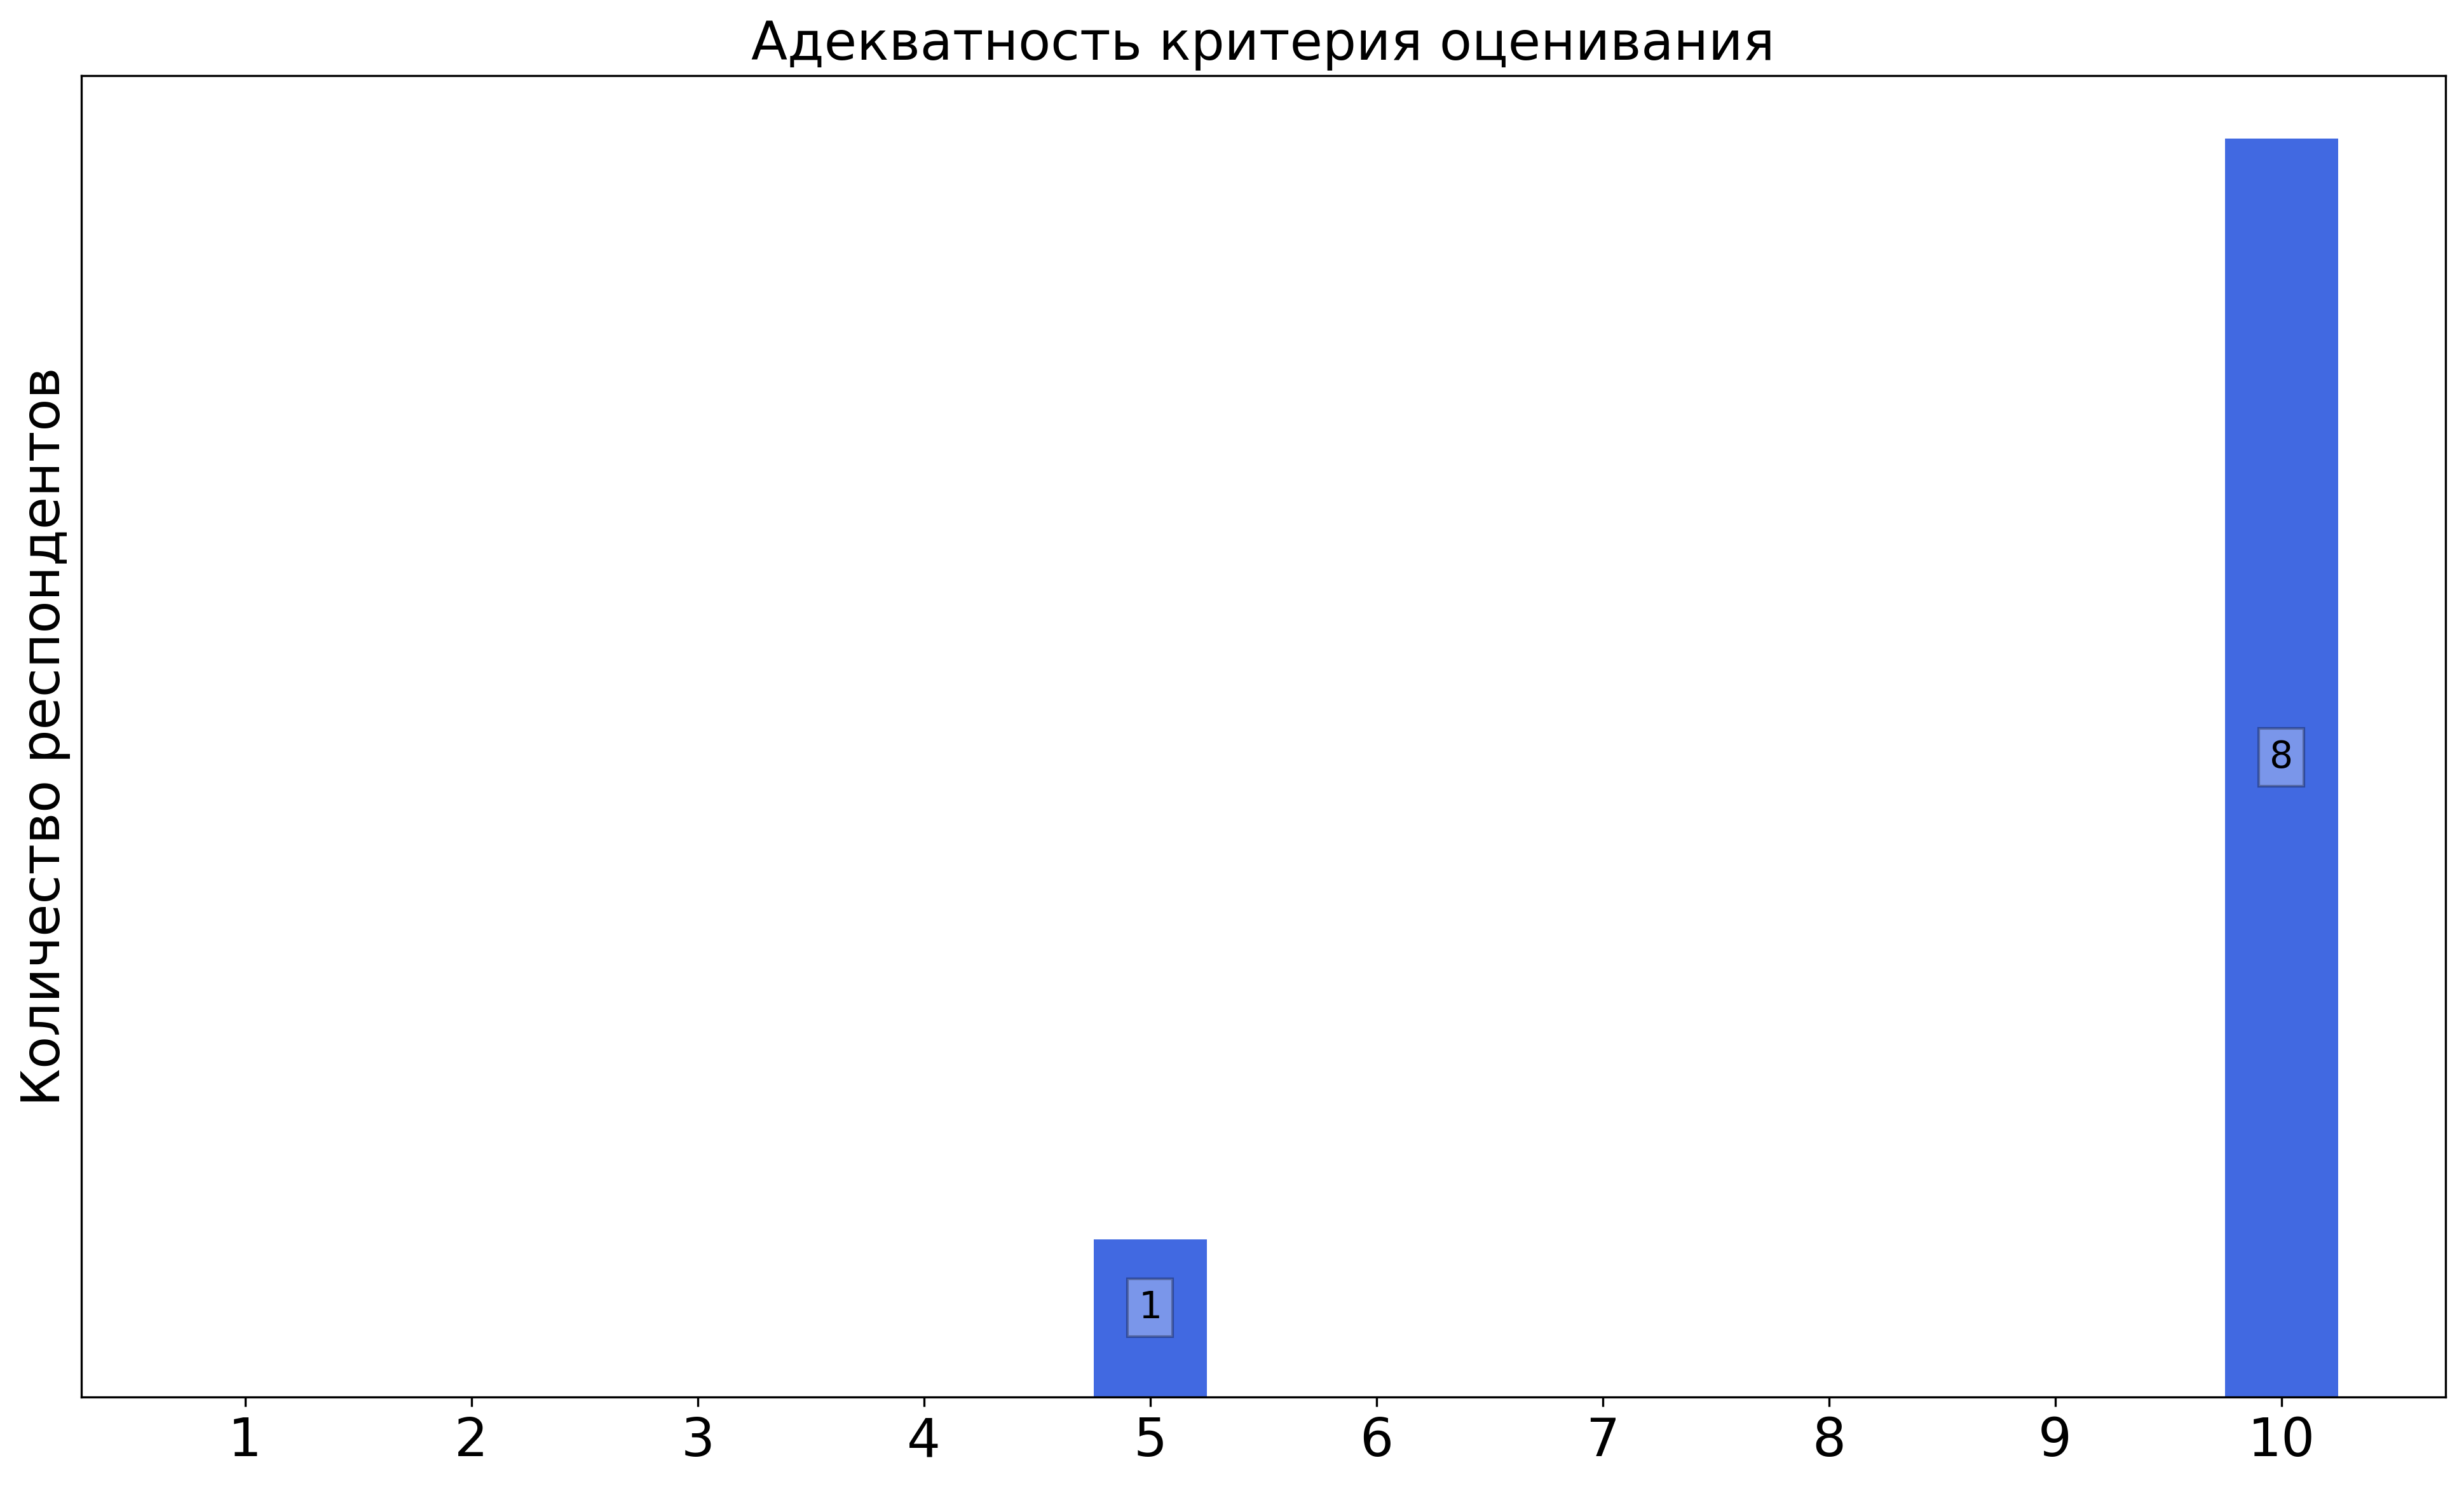
\includegraphics[width=\textwidth]{images/1 course/Общая физика - механика/labniks-marks-Суханова Е.В.-1.png}
			\end{subfigure}
			\begin{subfigure}[b]{0.45\textwidth}
				\centering
				\includegraphics[width=\textwidth]{images/1 course/Общая физика - механика/labniks-marks-Суханова Е.В.-2.png}
			\end{subfigure}
			\begin{subfigure}[b]{0.45\textwidth}
				\centering
				\includegraphics[width=\textwidth]{images/1 course/Общая физика - механика/labniks-marks-Суханова Е.В.-3.png}
			\end{subfigure}	
			\caption{Оценки респондентов о качестве преподавания лабораторных работ}
		\end{figure}

		\textbf{Комментарии студентов о преподавателе\protect\footnote{сохранены оригинальные орфография и пунктуация}}
            \begin{commentbox} 
                Топ с таким лабником  
            \end{commentbox} 
        
            \begin{commentbox} 
                Отвечает на все вопросы. Здорово объясняет материал. 
            \end{commentbox}


    \subsubsection{Отзыв студентов о лабораторных работах. Преподаватель: Титов А.С.}
        \begin{figure}[H]
            \centering
            \begin{subfigure}[b]{0.45\textwidth}
                \centering
                \includegraphics[width=\textwidth]{images/1 course/Общая физика - механика/labniks-marks-Титов А.С.-0.png}
            \end{subfigure}
            \begin{subfigure}[b]{0.45\textwidth}
                \centering
                \includegraphics[width=\textwidth]{images/1 course/Общая физика - механика/labniks-marks-Титов А.С.-1.png}
            \end{subfigure}
            \begin{subfigure}[b]{0.45\textwidth}
                \centering
                \includegraphics[width=\textwidth]{images/1 course/Общая физика - механика/labniks-marks-Титов А.С.-2.png}
            \end{subfigure}
            \begin{subfigure}[b]{0.45\textwidth}
                \centering
                \includegraphics[width=\textwidth]{images/1 course/Общая физика - механика/labniks-marks-Титов А.С.-3.png}
            \end{subfigure}	
            \caption{Оценки респондентов о качестве преподавания лабораторных работ}
        \end{figure}

        \textbf{Комментарии студентов о преподавателе\protect\footnote{сохранены оригинальные орфография и пунктуация}}
            \begin{commentbox} 
                Лабника нашей подгруппы нет (Чивилев), однако оценка идёт лабнику второй подгруппы, который в целом аналогичен  
            \end{commentbox} 
        
            \begin{commentbox} 
                тоже хороший тип 
            \end{commentbox} 
        
            \begin{commentbox} 
                В целом, лабораторный практикум 1 семестра основную миссию, на мой взгляд, выполнил - научил теоретические знания применять на практике, приобщил к методике и культуре ведения мининаучной работы  
            \end{commentbox}


    \subsubsection{Отзыв студентов о лабораторных работах. Преподаватель: Удалова А.Г.}
        \begin{figure}[H]
            \centering
            \begin{subfigure}[b]{0.45\textwidth}
                \centering
                \includegraphics[width=\textwidth]{images/1 course/Общая физика - механика/labniks-marks-Удалова А.Г.-0.png}
            \end{subfigure}
            \begin{subfigure}[b]{0.45\textwidth}
                \centering
                \includegraphics[width=\textwidth]{images/1 course/Общая физика - механика/labniks-marks-Удалова А.Г.-1.png}
            \end{subfigure}
            \begin{subfigure}[b]{0.45\textwidth}
                \centering
                \includegraphics[width=\textwidth]{images/1 course/Общая физика - механика/labniks-marks-Удалова А.Г.-2.png}
            \end{subfigure}
            \begin{subfigure}[b]{0.45\textwidth}
                \centering
                \includegraphics[width=\textwidth]{images/1 course/Общая физика - механика/labniks-marks-Удалова А.Г.-3.png}
            \end{subfigure}	
            \caption{Оценки респондентов о качестве преподавания лабораторных работ}
        \end{figure}

        \textbf{Комментарии студентов о преподавателе\protect\footnote{сохранены оригинальные орфография и пунктуация}}
            \begin{commentbox} 
                Ну наверное если с другими лабниками сравнивать, то сдача полайтовее. Хотя это вначале было, потом уже не сильно. Оценивает не сильно халявно, но минимум 7 я думаю всегда можно 
            \end{commentbox} 
        
            \begin{commentbox} 
                Мне позволила доделать пропущенную лабораторную, поэтому благодарен 
            \end{commentbox}


    \subsubsection{Отзыв студентов о лабораторных работах. Преподаватель: Ципенюк Д.Ю.}
        \begin{figure}[H]
            \centering
            \begin{subfigure}[b]{0.45\textwidth}
                \centering
                \includegraphics[width=\textwidth]{images/1 course/Общая физика - механика/labniks-marks-Ципенюк Д.Ю.-0.png}
            \end{subfigure}
            \begin{subfigure}[b]{0.45\textwidth}
                \centering
                \includegraphics[width=\textwidth]{images/1 course/Общая физика - механика/labniks-marks-Ципенюк Д.Ю.-1.png}
            \end{subfigure}
            \begin{subfigure}[b]{0.45\textwidth}
                \centering
                \includegraphics[width=\textwidth]{images/1 course/Общая физика - механика/labniks-marks-Ципенюк Д.Ю.-2.png}
            \end{subfigure}
            \begin{subfigure}[b]{0.45\textwidth}
                \centering
                \includegraphics[width=\textwidth]{images/1 course/Общая физика - механика/labniks-marks-Ципенюк Д.Ю.-3.png}
            \end{subfigure}	
            \caption{Оценки респондентов о качестве преподавания лабораторных работ}
        \end{figure}

        \textbf{Комментарии студентов о преподавателе\protect\footnote{сохранены оригинальные орфография и пунктуация}}
            \begin{commentbox} 
                Халява. Все, что он требует - чтобы были все пункты и ответ +- совпал, говорит, учит жизни, а научил быстро катать лабы в последний срок 
            \end{commentbox} 
        
            \begin{commentbox} 
                Главное что не запаривал, иногда интересно рассказывал про лабу, но в целом оценка на физтех-вики ему соотвествует. 
            \end{commentbox}


    \subsubsection{Отзыв студентов о лабораторных работах. Преподаватель: Черкасова Е.К.}
        \begin{figure}[H]
            \centering
            \begin{subfigure}[b]{0.45\textwidth}
                \centering
                \includegraphics[width=\textwidth]{images/1 course/Общая физика - механика/labniks-marks-Черкасова Е.К.-0.png}
            \end{subfigure}
            \begin{subfigure}[b]{0.45\textwidth}
                \centering
                \includegraphics[width=\textwidth]{images/1 course/Общая физика - механика/labniks-marks-Черкасова Е.К.-1.png}
            \end{subfigure}
            \begin{subfigure}[b]{0.45\textwidth}
                \centering
                \includegraphics[width=\textwidth]{images/1 course/Общая физика - механика/labniks-marks-Черкасова Е.К.-2.png}
            \end{subfigure}
            \begin{subfigure}[b]{0.45\textwidth}
                \centering
                \includegraphics[width=\textwidth]{images/1 course/Общая физика - механика/labniks-marks-Черкасова Е.К.-3.png}
            \end{subfigure}	
            \caption{Оценки респондентов о качестве преподавания лабораторных работ}
        \end{figure}

        \textbf{Комментарии студентов о преподавателе\protect\footnote{сохранены оригинальные орфография и пунктуация}}
            \begin{commentbox} 
                Приятная пожилая бабушка, лояльно оценивает, хоть и объясняет материал посредственно. 
            \end{commentbox} 
        
            \begin{commentbox} 
                Елена Константиновна не умеет объяснять, также она сказала, что мне надо было выбрать другой вуз - считаю это неправильным поведением преподавателя
            \end{commentbox}
    

    \subsubsection{Отзыв студентов о лабораторных работах. Преподаватель: Чернышов А.И.}
		\begin{figure}[H]
			\centering
			\begin{subfigure}[b]{0.45\textwidth}
				\centering
				\includegraphics[width=\textwidth]{images/1 course/Общая физика - механика/labniks-marks-Чернышов А.И.-0.png}
			\end{subfigure}
			\begin{subfigure}[b]{0.45\textwidth}
				\centering
				\includegraphics[width=\textwidth]{images/1 course/Общая физика - механика/labniks-marks-Чернышов А.И.-1.png}
			\end{subfigure}
			\begin{subfigure}[b]{0.45\textwidth}
				\centering
				\includegraphics[width=\textwidth]{images/1 course/Общая физика - механика/labniks-marks-Чернышов А.И.-2.png}
			\end{subfigure}
			\begin{subfigure}[b]{0.45\textwidth}
				\centering
				\includegraphics[width=\textwidth]{images/1 course/Общая физика - механика/labniks-marks-Чернышов А.И.-3.png}
			\end{subfigure}	
			\caption{Оценки респондентов о качестве преподавания лабораторных работ}
		\end{figure}

		\textbf{Комментарии студентов о преподавателе\protect\footnote{сохранены оригинальные орфография и пунктуация}}
            \begin{commentbox} 
                Крутой мужик, но строгий 
            \end{commentbox}

    
    \subsubsection{Отзыв студентов о лабораторных работах. Преподаватель: Яворский В.А.}
        \begin{figure}[H]
            \centering
            \begin{subfigure}[b]{0.45\textwidth}
                \centering
                \includegraphics[width=\textwidth]{images/1 course/Общая физика - механика/labniks-marks-Яворский В.А.-0.png}
            \end{subfigure}
            \begin{subfigure}[b]{0.45\textwidth}
                \centering
                \includegraphics[width=\textwidth]{images/1 course/Общая физика - механика/labniks-marks-Яворский В.А.-1.png}
            \end{subfigure}
            \begin{subfigure}[b]{0.45\textwidth}
                \centering
                \includegraphics[width=\textwidth]{images/1 course/Общая физика - механика/labniks-marks-Яворский В.А.-2.png}
            \end{subfigure}
            \begin{subfigure}[b]{0.45\textwidth}
                \centering
                \includegraphics[width=\textwidth]{images/1 course/Общая физика - механика/labniks-marks-Яворский В.А.-3.png}
            \end{subfigure}	
            \caption{Оценки респондентов о качестве преподавания лабораторных работ}
        \end{figure}

        \textbf{Комментарии студентов о преподавателе\protect\footnote{сохранены оригинальные орфография и пунктуация}}
            \begin{commentbox} 
                Научит качественно составлять отчеты. 
            \end{commentbox} 
        
            \begin{commentbox} 
                Хороший лабник, делает упор на знания студента, добросовестно выполняет свою работу 
            \end{commentbox} 
        
            \begin{commentbox} 
                Было сложно, но все в среднем сдали на 6-8. У меня 7 и я доволен, хотя препод очень требовательный 
            \end{commentbox} 


	\subsubsection{Прочие комментарии и предложения по улучшению курса}
        \begin{commentbox}
            Более фундаментальную физику хочу и больше одного семинара в неделю. Как-то тяжело идти голопом по Европам, а в данный момент по физике так. Один семинар одна тема, причём бывают не простые темы, в которых следует поглубже разобраться, но нет, следующих семинар другая тема
        \end{commentbox}

        \begin{commentbox}
            Честно говоря, хотелось бы другого лектора и семинариста
        \end{commentbox}

        \begin{commentbox}
            Уберите его ивтшникам пж, оставьте онли лабы для практики, там же принимают по теории, ну камон, я не хочу учить теорфиз
        \end{commentbox}

        \begin{commentbox}
            Несправедливое отношение к общей физике по сравнению с матаном. В 2 раза меньше лекций и в 2 раза меньше семинаров. А материала ни чуть не меньше. Опыта в решении задач очень мало. Буквально 1-2 задачи на 1 подход и все. Ну или это я тупой. Если бы добавили еще 1 семинар в неделю (вместо какого-нибудь бесполезного английского) было бы намного лучше. Понятное дело, что здесь все прогеры, в том числе и я, но экзы сдавать, госы тоже.
        \end{commentbox}

        \begin{commentbox}
            Да, в целом, все неплохо, только хотелось бы, чтобы в конце семестра не было ускоренного прохождения теории конца семестра
        \end{commentbox}
            